\PassOptionsToPackage{svgnames}{xcolor}
\documentclass[12pt]{article}
\usepackage{lmodern}

%%% The macro file where all style boxes are defined. 
%%% We should make sure we get this right before we distribute more widely.
%%% We should also clean this up a little. It's a working mess that I threw together as I needed
%%% Compiled by Thomas Wong, 2020


\usepackage{amsmath,amssymb,amsthm}%,import,dashrule}
\usepackage{graphicx}

\usepackage{multicol}
\usepackage{pifont}
\usepackage{amsfonts}
\usepackage{aliascnt}
\usepackage{fancyhdr}
\setlength{\headheight}{15pt}
\usepackage{enumitem}
\usepackage{lmodern,textcomp}%fonts

\usepackage{wasysym}


%\usepackage{gensymb} %for degree symbol

\usepackage{tikz}
\usetikzlibrary{fit,shapes}
\usetikzlibrary{plotmarks}
\usetikzlibrary{matrix,decorations.pathreplacing}
\usetikzlibrary{automata,positioning, calc}
\usepackage{pgfplots}

\usepackage[RPvoltages]{circuitikz} %drawing circuits
\usepackage[hypcap=false]{caption} %captioning figures
\renewcommand{\thefigure}{\thesection.\arabic{figure}}

\usepackage[titles]{tocloft}
\usepackage[paper=letterpaper,left=25mm,right=25mm,top=3cm,bottom=25mm]{geometry}
\usepackage{parskip}

\usepackage{colortbl}
\usepackage{color}   %May be necessary if you want to color links

\newcommand{\diag}{\operatorname{diag}}

\newcommand{\blue}{blue}
\newcommand{\red}{red}
\newcommand{\brown}{brown}
\newcommand{\green}{green}
\newcommand{\yellow}{yellow}
\newcommand{\gray}{gray!30}
\newcommand{\darkgray}{gray!60}
\newcommand{\black}{black}
\newcommand{\graphcolour}{red}
\newcommand{\white}{white}



\colorlet{lblue}{\blue!45!white}
\colorlet{lred}{\red!50!white}
\colorlet{lblue1}{\blue!10!white}
\colorlet{lred1}{\red!10!white}
\colorlet{lblue2}{\blue!45!white!50!\black}

% \newcommand{\vv}[1]{\underline{#1}}
 \newcommand{\vi}{\underline{i}}
 \newcommand{\vj}{\underline{j}}
 \newcommand{\vk}{\underline{k}}

%\newcommand{\vv}[1]{{\mathbf{#1}}}
%\newcommand{\vi}{\vv{i}}
%\newcommand{\vj}{\vv{j}}
%\newcommand{\vk}{\vv{k}}

\usepackage{hyperref}
\hypersetup{
    colorlinks=true, %set true if you want colored links
    linktoc=all,     %set to all if you want both sections and subsections linked
    linkcolor=lblue!50!black,  %choose some color if you want links to stand out
		filecolor=lblue!50!black,
		urlcolor=lblue!50!black,
		pdfnewwindow=true
}

\usepackage{polynom}
\usepackage[]{geometry}
\usepackage{array}
\usepackage{pdflscape}
\usepackage{rotating}

\usepackage{tcolorbox}
\usepackage{varwidth}
\tcbuselibrary{skins,breakable}
\usetikzlibrary{shadings,shadows}

\usepackage{chngcntr}%changes counter
\counterwithin*{figure}{section}

%creating QR codes
\usepackage{marginnote}
\usepackage{qrcode}

%writing code
\usepackage{verbatim}
%\usepackage{minted} % for code snippets
%\usepackage{listings}


% \lstset{
%   basicstyle=\ttfamily\small,
%   keywordstyle=\color{blue},
%   commentstyle=\color{gray},
%   stringstyle=\color{orange},
%   breaklines=true,
%   frame=single,
%   showstringspaces=false
% }

\renewcommand{\familydefault}{\sfdefault}

%\setcounter{section}{-1}
%\setlength{\cftbeforechapskip}{2ex}
\setlength{\cftbeforesecskip}{0.1ex}
\setcounter{tocdepth}{2}
\pagestyle{fancyplain}
\numberwithin{equation}{section}
 
\theoremstyle{definition}
\newtheorem{cou}{counting}[section]

\newaliascnt{df}{cou}
\newaliascnt{thm}{cou}
\newaliascnt{rem}{cou}
\newaliascnt{example}{cou}
\newaliascnt{exercise}{cou}

%\newtheorem{df}[df]{Definition}
%\newtheorem{thm}[thm]{Theorem}
%\newtheorem{example}[example]{Example}
%\newtheorem{exercise}[exercise]{Exercise}

%\newtcolorbox[use counter=thm,number within=section]{thm}[2][]{%
%fonttitle=\bfseries,
%title= Theorem \thethm\; #2,#1}

\newtcolorbox[use counter=exercise,number within=section]{exercise}[2][]{%
fonttitle=\bfseries,
colbacktitle=lblue!60!black,
title= Exercise \theexercise\; #2,#1}

\newtcolorbox[use counter=rem,number within=section]{rem}[2][]{enhanced,
colbacktitle=\blue,
boxrule=0.2mm,
attach boxed title to top left={xshift=1cm,yshift*=1mm-\tcboxedtitleheight},
varwidth boxed title*=-3cm,
boxed title style={frame code={
\path[fill=tcbcolback!30!black]
([yshift=-1mm,xshift=-1mm]frame.north west)
arc[start angle=0,end angle=180,radius=1mm]
([yshift=-1mm,xshift=1mm]frame.north east)
arc[start angle=180,end angle=0,radius=1mm];
\path[left color=tcbcolback!60!black,right color=tcbcolback!60!black,middle color=tcbcolback!60!black]
([xshift=-2mm]frame.north west) -- ([xshift=2mm]frame.north east)
[rounded corners=1mm]-- ([xshift=1mm,yshift=-1mm]frame.north east)
-- (frame.south east) -- (frame.south west)
-- ([xshift=-1mm,yshift=-1mm]frame.north west)
[sharp corners]-- cycle;
}
,interior engine=empty,
},
fonttitle=\bfseries,
title=Remark \therem\; {#2},#1}



\newtcolorbox[use counter=df,number within=section]{df}[2][]{enhanced,
colbacktitle=\blue,
boxrule=0.2mm,
attach boxed title to top left={xshift=1cm,yshift*=1mm-\tcboxedtitleheight},
varwidth boxed title*=-3cm,
boxed title style={frame code={
\path[fill=tcbcolback!30!black]
([yshift=-1mm,xshift=-1mm]frame.north west)
arc[start angle=0,end angle=180,radius=1mm]
([yshift=-1mm,xshift=1mm]frame.north east)
arc[start angle=180,end angle=0,radius=1mm];
\path[left color=tcbcolback!60!black,right color=tcbcolback!60!black,middle color=tcbcolback!60!black]
([xshift=-2mm]frame.north west) -- ([xshift=2mm]frame.north east)
[rounded corners=1mm]-- ([xshift=1mm,yshift=-1mm]frame.north east)
-- (frame.south east) -- (frame.south west)
-- ([xshift=-1mm,yshift=-1mm]frame.north west)
[sharp corners]-- cycle;
}
,interior engine=empty,
},
fonttitle=\bfseries,
title=Definition \thedf\; {#2},#1}

\newtcolorbox[use counter=thm,number within=section]{thm}[2][]{
enhanced,
%skin=enhancedlast jigsaw,
attach boxed title to top left={xshift=-4mm,yshift=-0.5mm},
fonttitle=\bfseries\sffamily,varwidth boxed title=0.7\linewidth,
colbacktitle=lblue!60!black,colframe=lblue!60!black,
%interior style={top color=lblue1,bottom color=lred1},
boxed title style={empty,arc=0pt,outer arc=0pt,boxrule=0pt},
underlay boxed title={
\fill[lblue!80!black] (title.north west) -- (title.north east)
-- +(\tcboxedtitleheight-1mm,-\tcboxedtitleheight+1mm)
-- ([xshift=4mm,yshift=0.5mm]frame.north east) -- +(0mm,-1mm)
-- (title.south west) -- cycle;
\fill[lblue2] ([yshift=-0.5mm]frame.north west)
-- +(-0.4,0) -- +(0,-0.3) -- cycle;
\fill[lblue2] ([yshift=-0.5mm]frame.north east)
-- +(0,-0.3) -- +(0.4,0) -- cycle; 
},
title= Theorem \thethm\; {#2},#1}

%\thetcbcounter

\newtcolorbox[use counter=example,number within=section]{example}[1][]{%
empty,title={Example \theexample},attach boxed title to top left,
boxed title style={empty,size=minimal,toprule=2pt,top=4pt,
overlay={\draw[lblue!60!black,line width=2pt]
([yshift=-1pt]frame.north west)--([yshift=-1pt]frame.north east);}},
coltitle=lblue!60!black,fonttitle=\bfseries,
before=\par\medskip\noindent,parbox=false,boxsep=0pt,left=0pt,right=3mm,top=4pt,
breakable,pad at break*=0mm,vfill before first,
overlay unbroken={\draw[lblue,line width=1pt]
([yshift=-1pt]title.north east)--([xshift=-0.5pt,yshift=-1pt]title.north-|frame.east)
--([xshift=-0.5pt]frame.south east)--(frame.south west); },
overlay first={\draw[lblue,line width=1pt]
([yshift=-1pt]title.north east)--([xshift=-0.5pt,yshift=-1pt]title.north-|frame.east)
--([xshift=-0.5pt]frame.south east); },
overlay middle={\draw[lblue,line width=1pt] ([xshift=-0.5pt]frame.north east)
--([xshift=-0.5pt]frame.south east); },
overlay last={\draw[lblue,line width=1pt] ([xshift=-0.5pt]frame.north east)
--([xshift=-0.5pt]frame.south east)--(frame.south west);},#1%
}

\aliascntresetthe{df}
\aliascntresetthe{rem}
\aliascntresetthe{thm}
\aliascntresetthe{example}
\aliascntresetthe{exercise}

\newcommand*{\dfautorefname}{Definition}
\newcommand*{\remautorefname}{Remark}
\newcommand*{\thmautorefname}{Theorem}
\newcommand*{\exampleautorefname}{Example}
\newcommand*{\exerciseautorefname}{Exercise}
%\renewcommand*{\sectionautorefname}{Section}
%\renewcommand*{\subsectionautorefname}{Section}

\newtcolorbox{solution}{
empty,
breakable,left=5mm,right=5mm,
borderline west={1mm}{0pt}{\blue!60!black},
borderline east={1mm}{0pt}{\blue!60!black},
title= {Solution:\:\:},
attach title to upper,
fonttitle=\bfseries,
coltitle = black,
}

\newcommand\encircle[1]{%
  \tikz[baseline=(X.base)] 
    \node (X) [draw, shape=circle, inner sep=0] {\strut #1};}

\renewcommand*\contentsname{Contents}

\newcommand{\sitem}[1]{\begin{itemize}[noitemsep,nolistsep] #1 \end{itemize}}
\newcommand{\senum}[1]{\begin{enumerate}[noitemsep,nolistsep] #1 \end{enumerate}}
\newcommand{\tom}[1]{({\bf Tom:} \emph{#1})}
\newcommand{\defn}[1]{\begin{center} \emph{#1} \end{center}}
\newcommand{\pic}[2][0.7]{
\begin{center}
	\includegraphics[width=#1\textwidth]{images/#2}
\end{center}
}

%setting QR links
\newcommand{\qrlink}[2][]{\marginnote{\qrcode[height=0.9\marginparwidth,#1]{#2}}}%[-0.5cm]}



%\newcommand{\degs}{\degree}
\newcommand{\degs}{^\circ}

%\AtBeginDocument{%
% \abovedisplayshortskip=0pt
% \belowdisplayskip=0pt
% \belowdisplayshortskip=0pt
%}

\makeatletter
\newcommand\footnoteref[1]{\protected@xdef\@thefnmark{\ref{#1}}\@footnotemark}
\makeatother

\newcommand{\caution}{
\begin{tikzpicture}[scale=1,baseline=0cm] %\scriptsize
	\path[rounded corners,draw=\yellow!50!\red,fill=none,thick]  (-0.25,0) -- (0.25,0) -- (0,0.433) -- cycle;
	\path[rounded corners=0.5mm,draw=none,fill=\yellow!60,thick]  (-0.19,0.04) -- (0.19,0.04) -- (0,0.37) -- cycle;
	\draw[draw=\yellow!20!\red,fill=none,thick]  (0,0.07) -- (0,0.1)  (0,0.12) -- (0,0.28);
\end{tikzpicture}}

\newcommand{\question}{
\tikz[baseline=(wi.base)]{
\node[fill=black,rotate=45,inner sep=.1ex,text height=1.8ex,text width=1.8ex] {};
\node[font=\color{white}] (wi) {?};
}	
}

\usepackage{xcolor}

\newcommand{\hl}[1]{%
  \colorbox{\red!50}{#1}}

%%
\usepackage{pgfplots,mathtools}
\pgfplotsset{compat=1.7}
\pgfmathdeclarefunction{gauss}{2}{\pgfmathparse{1/(#2*sqrt(2*pi))*exp(-((x-#1)^2)/(2*#2^2))}%
}

%%Importing tutorial questions
\usepackage{catchfilebetweentags}
\newtoks\temptoken

\usepackage[lastexercise,answerdelayed]{exercise}  
\renewcommand{\QuestionNB}{(\alph{Question})\ }
%\renewcommand{\subQuestionNB}{\roman{subQuestion})}
\renewcommand{\ExerciseHeader}{\textbf{\theExercise.} \hspace{-4mm} \textbf{\ExerciseHeaderTitle}}
\renewcommand{\AnswerHeader}{\textbf{\theExercise.}  \hspace{-4mm} \textbf{\ExerciseHeaderTitle}}
\setlength{\ExerciseSkipBefore}{-0.8ex}
\setlength{\AnswerSkipBefore}{-3ex}
\setlength{\QuestionBefore}{-1ex}

\renewcounter{Exercise}[subsection]% Reset counter.
\renewcommand{\theExercise}{\thesubsection.\arabic{Exercise}}%

\newcommand{\multicolq}[2][3]{
\begin{multicols*}{#1}
#2
\EndCurrentQuestion
\end{multicols*}
}

\newcommand{\multicolqq}[2][3]{
\begin{multicols*}{#1}
#2
\EndCurrentsubQuestion
\end{multicols*}
}

\newcommand{\tutorial}[1]{
\subsubsection*{Tutorial Exercises for \thesubsection} 

\medskip 

\ExecuteMetaData[\tutorialsheetlocation]{#1}

\vspace*{-1ex} \hspace*{\fill} \hyperref[A:answers]{(Answers)}
}

%%%%%%%Alex's Stuff%%%%%%%%%%%%

\newcommand{\bbA}{{\mathbb A}}
\newcommand{\bbB}{{\mathbb B}}
\newcommand{\bbC}{{\mathbb C}}
\newcommand{\bbD}{{\mathbb D}}
\newcommand{\bbE}{{\mathbb E}}
\newcommand{\bbF}{{\mathbb F}}
\newcommand{\bbG}{{\mathbb G}}
\newcommand{\bbH}{{\mathbb H}}
\newcommand{\bbI}{{\mathbb I}}
\newcommand{\bbJ}{{\mathbb J}}
\newcommand{\bbK}{{\mathbb K}}
\newcommand{\bbL}{{\mathbb L}}
\newcommand{\bbM}{{\mathbb M}}
\newcommand{\bbN}{{\mathbb N}}
\newcommand{\bbO}{{\mathbb O}}
\newcommand{\bbP}{{\mathbb P}}
\newcommand{\bbQ}{{\mathbb Q}}
\newcommand{\bbR}{{\mathbb R}}
\newcommand{\bbS}{{\mathbb S}}
\newcommand{\bbT}{{\mathbb T}}
\newcommand{\bbU}{{\mathbb U}}
\newcommand{\bbV}{{\mathbb V}}
\newcommand{\bbW}{{\mathbb W}}
\newcommand{\bbX}{{\mathbb X}}
\newcommand{\bbY}{{\mathbb Y}}
\newcommand{\bbZ}{{\mathbb Z}}

\newcommand{\cA}{{\mathcal A}}
\newcommand{\cB}{{\mathcal B}}
\newcommand{\cC}{{\mathcal C}}
\newcommand{\cD}{{\mathcal D}}
\newcommand{\cE}{{\mathcal E}}
\newcommand{\cF}{{\mathcal F}}
\newcommand{\cG}{{\mathcal G}}
\newcommand{\cH}{{\mathcal H}}
\newcommand{\cI}{{\mathcal I}}
\newcommand{\cJ}{{\mathcal J}}
\newcommand{\cK}{{\mathcal K}}
\newcommand{\cL}{{\mathcal L}}
\newcommand{\cM}{{\mathcal M}}
\newcommand{\cN}{{\mathcal N}}
\newcommand{\cO}{{\mathcal O}}
\newcommand{\cP}{{\mathcal P}}
\newcommand{\cQ}{{\mathcal Q}}
\newcommand{\cR}{{\mathcal R}}
\newcommand{\cS}{{\mathcal S}}
\newcommand{\cT}{{\mathcal T}}
\newcommand{\cU}{{\mathcal U}}
\newcommand{\cV}{{\mathcal V}}
\newcommand{\cW}{{\mathcal W}}
\newcommand{\cX}{{\mathcal X}}
\newcommand{\cY}{{\mathcal Y}}
\newcommand{\cZ}{{\mathcal Z}}

\newcommand{\fra}{{\mathfrak a}}
\newcommand{\frb}{{\mathfrak b}}
\newcommand{\frc}{{\mathfrak c}}
\newcommand{\frd}{{\mathfrak d}}
\newcommand{\fre}{{\mathfrak e}}
\newcommand{\frf}{{\mathfrak f}}
\newcommand{\frg}{{\mathfrak g}}
\newcommand{\frh}{{\mathfrak h}}
\newcommand{\fri}{{\mathfrak i}}
\newcommand{\frj}{{\mathfrak j}}
\newcommand{\frk}{{\mathfrak k}}
\newcommand{\frl}{{\mathfrak l}}
%\renewcommand{\frm}{{\mathfrak m}}
\newcommand{\frn}{{\mathfrak n}}
\newcommand{\fro}{{\mathfrak o}}
\newcommand{\frp}{{\mathfrak p}}

\newcommand{\frr}{{\mathfrak r}}
\newcommand{\frs}{{\mathfrak s}}
\newcommand{\frt}{{\mathfrak t}}
\newcommand{\fru}{{\mathfrak u}}
\newcommand{\frv}{{\mathfrak v}}
\newcommand{\frw}{{\mathfrak w}}
\newcommand{\frx}{{\mathfrak x}}
\newcommand{\fry}{{\mathfrak y}}
\newcommand{\frz}{{\mathfrak z}}


\newcommand{\frA}{{\mathfrak A}}
\newcommand{\frB}{{\mathfrak B}}
\newcommand{\frC}{{\mathfrak C}}
\newcommand{\frD}{{\mathfrak D}}
\newcommand{\frE}{{\mathfrak E}}
\newcommand{\frF}{{\mathfrak F}}
\newcommand{\frG}{{\mathfrak G}}
\newcommand{\frH}{{\mathfrak H}}
\newcommand{\frI}{{\mathfrak I}}
\newcommand{\frJ}{{\mathfrak J}}
\newcommand{\frK}{{\mathfrak K}}
\newcommand{\frL}{{\mathfrak L}}
\newcommand{\frM}{{\mathfrak M}}
\newcommand{\frN}{{\mathfrak N}}
\newcommand{\frO}{{\mathfrak O}}
\newcommand{\frP}{{\mathfrak P}}
\newcommand{\frQ}{{\mathfrak Q}}
\newcommand{\frR}{{\mathfrak R}}
\newcommand{\frS}{{\mathfrak S}}
\newcommand{\frT}{{\mathfrak T}}
\newcommand{\frU}{{\mathfrak U}}
\newcommand{\frV}{{\mathfrak V}}
\newcommand{\frW}{{\mathfrak W}}
\newcommand{\frX}{{\mathfrak X}}
\newcommand{\frY}{{\mathfrak Y}}
\newcommand{\frZ}{{\mathfrak Z}}

\newcommand{\lra}{\longrightarrow}
\newcommand{\ra}{\rightarrow}
\newcommand{\Ra}{\Rightarrow}
\newcommand{\La}{\Leftarrow}
\newcommand{\Lra}{\Leftrightarrow}
\newcommand{\hra}{\hookrightarrow}
\newcommand{\eps}{\varepsilon}
\newcommand{\Vxi}{V_{\cU, \varepsilon}(\xi)}
\newcommand{\Veta}{V_U(\eta)}



\newcommand{\xh}{\hat{x}}
\newcommand{\mata}[1]{\left(\begin{array}{cc}#1\end{array}\right)}
\newcommand{\asu}{\mathfrak{su}}
\newcommand{\sSU}{\mathsf{SU}}
\newcommand{\sPSU}{\mathsf{P SU}}
\newcommand{\CC}{\mathcal{C}}
\newcommand{\CCC}{\mathscr{C}}
\newcommand{\CCL}{\mathscr{L}}
%\newcommand{\CD}{\mathcal{D}}
\newcommand{\CCD}{\mathscr{D}}
\newcommand{\CCDb}{\bar{\mathscr{D}}}
\newcommand{\CF}{\mathcal{F}}
\newcommand{\CCF}{\mathscr{F}}
\newcommand{\CG}{\mathcal{G}}
\newcommand{\CCG}{\mathscr{G}}
\newcommand{\CH}{\mathcal{H}}
\newcommand{\CCH}{\mathscr{H}}
\newcommand{\CI}{\mathcal{I}}
\newcommand{\CJ}{\mathcal{J}}
\newcommand{\CK}{\mathcal{K}}
\newcommand{\sU}{\mathsf{U}}
\newcommand{\sSL}{\mathsf{SL}}
\newcommand{\sGL}{\mathsf{GL}}
\newcommand{\sMat}{\mathsf{Mat}}
\newcommand{\sDiag}{\mathsf{Diag}}
\newcommand{\sO}{\mathsf{O}}
\newcommand{\de}{\mathrm{e}}     			% Euler's number
\newcommand{\rk}{{\rm rk}}     			% imaginary unit
\newcommand{\di}{\mathrm{i}}     			% imaginary unit
\newcommand{\sSO}{\mathsf{SO}}
\newcommand{\sS}{\mathsf{S}}
\newcommand{\sSpin}{\mathsf{Spin}}
\newcommand{\sPin}{\mathsf{Pin}}
\newcommand{\Det}{\hbox{Det}}
\newcommand{\hbo}{\hbox to 1 true cm {\hfill } }
\newcommand{\RZ}{\mathds{Z}}     			% ring of integers
%\renewcommand{\span}{{\rm span}}
\newcommand{\tr}{\hbox{tr}}
\newcommand{\Tr}{\hbox{Tr}}
\newcommand{\slc}{$\sSL(2,\mathbb{C})$}
\newcommand{\dalpha}{{\dot\alpha}}
\newcommand{\dbeta}{{\dot\beta}}
%\newcommand{\eps}{{\varepsilon}}			% antisymmetric tensors
\renewcommand{\sup}[2]{\{\![#1,#2]\!\}}
\newcommand{\vectt}[2]{\left(\begin{array}{c} #1 \\ #2 \end{array}\right)}
\newcommand{\vecttt}[3]{\left(\begin{array}{c} #1 \\ #2 \\ #3\end{array}\right)}
\newcommand{\vectttt}[4]{\left(\begin{array}{c} #1 \\ #2 \\ #3 \\ #4\end{array}\right)}
\newcommand{\vecttdt}[3]{\left(\begin{array}{c} #1 \\ #2 \\ \vdots \\ #3\end{array}\right)}
\newcommand{\matrixbig}[3]{\left(\begin{array}{cccc} #1_{11} & #1_{12} & \ldots & #1_{1#3} \\
		#1_{21} & #1_{22} & \ldots & #1_{2#3} \\
		\vdots & \vdots &  & \vdots \\
		#1_{#2 1} & #1_{#2 2} & \ldots & #1_{#2 #3}\end{array}\right)}
\newcommand{\matrixsmall}[3]{\left(\begin{array}{ccc} #1_{11} & \ldots & #1_{1#3} \\
		\vdots &   & \vdots \\
		#1_{#2 1} & \ldots & #1_{#2 #3}\end{array}\right)}
\newcommand{\vectbig}[2]{\left(\begin{array}{c} #1_1 \\ #1_2 \\ \vdots \\ #1_#2\end{array}\right)}
\newcommand{\ggama}{{\boldsymbol\gamma}}
\newcommand{\un}[1]{\underline{#1}}
\newcommand{\Eins}{\mathdsss{1}}
%\newcommand{\dd}{\mathrm{d}}     			% total differential
\newcommand{\bracket}[2]{\bra{#1}\,#2\rangle} % Dirac inner product
\newcommand{\bra}[1]{\langle\,#1\,|}          % Dirac bra
\newcommand{\ket}[1]{|\,#1\,\rangle}          % Dirac Ket
\newcommand{\linv}{{\triangle}^{-1}}      % inv. Laplacian
\newcommand{\ud}{\mathrm{d}}
%\newcommand{\remark}[1]{}     				% remark
\newcommand{\ewith}{~~~\mbox{with}~~~}
\newcommand{\eand}{~~~\mbox{and}~~~}
\newcommand{\eor}{~~~\mbox{or}~~~}
\newcommand{\nextyear}[1]{}     				% remark
\newcommand{\pathD}{\mathcal{D}}
\newcommand{\e}{\mathrm{e}}		% exponential e
\newcommand{\x}{\boldsymbol{x}}		% vector x
\newcommand{\NN}{\mathds{N}}     			% set of natural numbers
\newcommand{\unit}{\mathds{1}}   			% identity map/matrix
\newcommand{\y}{\boldsymbol{y}}		% vector y
\newcommand{\z}{\boldsymbol{z}}		% vector z
\newcommand{\av}{\vec{a}}		% vector v
\newcommand{\bv}{\vec{b}}		% vector v
\newcommand{\cv}{\vec{c}}		% vector v
\newcommand{\ev}{\vec{e}}		% vector v
\newcommand{\fv}{\vec{f}}	
\newcommand{\nv}{\vec{0}}
\newcommand{\pv}{\vec{p}}		% vector v
\newcommand{\rv}{\vec{r}}		% vector v
\newcommand{\sv}{\vec{s}}		% vector v
\newcommand{\uv}{\vec{u}}		% vector v
\newcommand{\vv}{\vec{v}}		% vector v
\newcommand{\wv}{\vec{w}}		% vector v
\newcommand{\xv}{\vec{x}}		% vector v
\newcommand{\yv}{\vec{y}}		% vector v
\newcommand{\zv}{\vec{z}}	
\renewcommand{\u}{\boldsymbol{u}}
\newcommand{\p}{\boldsymbol{p}}		% vector p
\newcommand{\q}{\boldsymbol{q}}		% vector q
\renewcommand{\r}{\boldsymbol{r}}		% vector q
%\newcommand{\E}{\boldsymbol{E}}
\newcommand{\A}{\boldsymbol{A}}
\newcommand{\J}{\boldsymbol{J}}
%\newcommand{\Q}{\mathcal{Q}}
\newcommand{\FR}{\mathds{R}} 
\newcommand{\FZ}{\mathds{Z}} 
\newcommand{\FN}{\mathds{N}}     			% field of real numbers
\newcommand{\FC}{\mathds{C}}     			% field of complex numbers
\newcommand{\CN}{\mathcal{N}}   
\newcommand{\CP}{\mathcal{P}}   	
\newcommand{\CB}{\mathcal{B}} 
\newcommand{\CL}{\mathcal{L}}   		% field of real numbers
%\newcommand{\eolec}[2]{}
%\newcommand{\eolec}[2]{\marginpar{~~~~~#1\\[-0.3cm]\rule{50pt}{0.4pt}\\\phantom{~~~~~}#2}}
%\newcommand{\tut}[1]{\marginpar{Tutorial #1\\[-0.3cm]\rule{50pt}{0.4pt}\\[-0.45cm]\rule{50pt}{0.4pt}}}

\usepackage{dsfont}

%\newcommand{\hey}[1]{{\color{TealBlue}(#1)}}

\newcommand{\elt}[1]{\stackrel{\footnotesize{#1}}{\rightsquigarrow}}
\newcommand{\melt}[1]{\stackrel{\begin{smallmatrix}#1\end{smallmatrix}}{\rightsquigarrow}}
		% Common macros for all files.
%%%%%%%%%%% NOTATION SHORTCUTS %%%%%%%%%%%%%%%%%%%
%
%  Consistent set of notation shortcuts usable in all directories.
%  


% Tikz shortcuts
\usepackage{pgf}
\usepackage{tikz} 
\usetikzlibrary{arrows,decorations.markings}
\tikzstyle{arrowmid}[0.65]=[decoration={markings,mark=at position #1 with {\arrow{>}}}, postaction={decorate}] 
 \tikzstyle{dot}[1.5]=[circle,fill,draw,minimum size=#1mm,inner sep=0pt]  


\def\checkmark{\tikz\fill[scale=0.4](0,.35) -- (.25,0) -- (1,.7) -- (.25,.15) -- cycle;} 

\newcommand{\ddx}[1][]{\frac{{\rm d} {#1}}{{\rm d}x}}
\newcommand{\dd}[1][]{\frac{{\rm d}}{{\rm d} #1}}
\newcommand{\dydx}[2][x]{\frac{{\rm d} #2}{{\rm d} #1}}
\newcommand{\ddt}[1][]{\frac{{\rm d} {#1}}{{\rm d}t}}
\newcommand{\pve}{{\rm +ve}}
\newcommand{\nve}{{\rm -ve}}


% Blackboard bold shortcuts
\newcommand{\Z}{\mathbb{Z}}
\newcommand{\Q}{\mathbb{Q}}
\newcommand{\C}{\mathbb{C}}
\newcommand{\N}{\mathbb{N}}
\newcommand{\R}{\mathbb{R}}
\newcommand{\E}{\mathbb{E}}

% Operators
\newcommand{\arccosec}{\operatorname{arccosec}}
\newcommand{\cosec}{\operatorname{cosec}}
\newcommand{\range}{\operatorname{range}}
\newcommand{\dom}{\operatorname{dom}}
\newcommand{\codom}{\operatorname{codom}}
\newcommand{\var}{\operatorname{Var}}

% Calculus shortcuts
%\newcommand{\dydx}{\dfrac{dy}{dx}}
\newcommand{\dydt}{\dfrac{dy}{dt}}
\newcommand{\dxdt}{\dfrac{dx}{dt}}
\newcommand{\dudx}{\dfrac{du}{dx}}
\newcommand{\dudy}{\dfrac{du}{dy}}
\newcommand{\dvdx}{\dfrac{dv}{dx}}
\newcommand{\ddydx}{\dfrac{d^{2}y}{dx^{2}}}
\newcommand{\ddydt}{\dfrac{d^{2}y}{dt^{2}}}
\newcommand{\dddydx}{\dfrac{d^{3}y}{dx^{3}}}
\newcommand{\ddy}{\dfrac{d}{dy}}
\newcommand{\dx}{\,\mathrm{d}x}
\newcommand{\dy}{\,\mathrm{d}y}
\newcommand{\du}{\,\mathrm{d}u}
\newcommand{\dv}{\,\mathrm{d}v}

%Complex numbers
%\newcommand{\degs}{^\circ}
\newcommand{\RE}[1]{\mathrm{Re}\left( #1 \right)}
\newcommand{\IM}[1]{\mathrm{Im}\left( #1 \right)}
\newcommand{\conj}[1]{\overline{#1}}
\newcommand{\abs}[1]{\left| #1 \right|}
\newcommand{\Arg}[1]{\text{Arg}\left( #1 \right)}
\newcommand{\Log}{\text{Log}}

\newcommand{\dist}{\operatorname{dist}}		% Common notation shortcuts for all subject files.

%\newcommand{\tutorialsheetlocation}{TutorialContent.tex}


\newcommand{\secbreak}{\pagebreak}

\usepackage{comment}

\usepackage{graphicx}

\lhead{F17ZD}
\chead{}
\rhead{\nouppercase{\leftmark}}
\lfoot{}
\cfoot{\thepage}
\rfoot{}



\begin{document}

\setcounter{page}{0}
\thispagestyle{empty} 
\centerline{\Large \bf F17ZD} \vspace{6mm} 
\centerline{\Large\bf Mathematics for Data Scientists 4} \vspace{6mm} 
\centerline{\Large \bf Course Notes} \vspace{6mm} 
\centerline{\bf Semester 2, 2025/26}

\vspace{80pt}

\begin{center}
\begin{tikzpicture}[scale=1.6]
\draw[thick,->] (0,0) -- (1,3) node[pos=0.5, below right,scale=0.7]{$\av$};
\draw[thick,->] (0,0) -- (4,0) node[pos=0.5, below,scale=0.7]{$\bv$};
\draw[thick,->] (0,0) -- (2,1) node[pos=0.5, above left,scale=0.7]{$\cv$};
\draw[-] (4,0) -- (6,1) ;
\draw[-] (2,1) -- (6,1) ;

\draw[-] (1,3) -- (5,3) ;
\draw[-] (1,3) -- (3,4) ;
\draw[-] (5,3) -- (7,4) ;
\draw[-] (3,4) -- (7,4) ;

\draw[-] (4,0) -- (5,3) ;
\draw[-] (2,1) -- (3,4) ;
\draw[-] (6,1) -- (7,4) ;

\draw[dashed] (0,0) -- (0,5);
\draw[dashed] (0,3) -- (1,3) node [pos=0, left,scale=0.7]{$h$};
\draw[]  (0,1) arc (90:71.56:1) node[pos=0.5, above, scale=0.7]{$\phi$};
\end{tikzpicture}
\end{center}
  

\vspace{80pt}

{\large\bf Name: $\rule{14cm}{0.15mm}$}
%{\large\bf Name: $\rule{12.2cm}{0.15mm}$}

%\clearpage
\thispagestyle{empty} 
%Some helpful tips:
%\begin{itemize}
%\item \question - Questions with this symbol are left as an exercise for the student or will be completed during the live sessions.
%\item \caution - Pay close attention to these points
%\item QR codes (and other elements) in the PDF version of these notes are hyperlinked
%\end{itemize}

\vspace*{\fill}
\parbox{0.9\textwidth}{\small
\begin{itemize}[noitemsep,nolistsep]
\item Copyright Heriot Watt University 2026. All rights reserved. For use of students of Xidian and Heriot Watt Universities enrolled in the course F17ZD.
\item Based on notes by Jack Carr, Des Johnston, Alex Martin and Thomas Wong.
\end{itemize}
}
\newpage 

\tableofcontents

%\newpage
%\setcounter{section}{-1}
%\section{Changes so far}

\tom{this section is for internal circulation and will be omitted in the student version}

General changes include:
\begin{itemize}
\item \textbf{Formatting:} Used environments for theorems, definitions, examples, exercise, and solutions. Each visually different so that it works with black/white print.
\item \textbf{Wording:} Removed words that cause ambiguity, such as \emph{try} or \emph{guess}. Removed words such as \emph{clearly} or \emph{easily}.
\item \textbf{Details:} Included addition definitions/theorems to separate, clarify ideas, and improve mathematical rigour.
\item \textbf{Updating tex:} Mostly behind the scenes stuff. Convert tex to more use modern environments. Try to use less manual spacing
\item \textbf{Pictures:} Converted graphs to tikz (where possible)
\item \textbf{Notation:} Changed $\sin^{-1}$ to $\arcsin$. Consistency with bracketing
\item \textbf{Hyperlink elements:} when referring to previously mentioned examples and general navigation
\item \textbf{QR codes:} for increased accessibility to interactive elements (mostly desmos).
\item \textbf{Typesetting style:} Exercise solutions formatting to resemble written solutions
\item \textbf{Footnotes:} Added in places for relevant additional notes or caveats
\item \textbf{Tutorial:} Questions added at the end of relevant sections. Answers at the end of document. Questions/Answers hyperlinked.
\end{itemize}

\subsection{Chapter 1: Applications of Differentiation}
\begin{itemize}
\item Added point-slope formula.
\item The \question symbol to means solutions left for lectures or as an exercise.
\item Ordering change: Product rule, quotient rule, chain rule (consistent with F17XA)
\item Ordering change: Linear approximation before Maclaurin and Taylor
\item Introduced notation $L(x)$ for linear approximation
\item Differentiate between Polynomial/series
\item Ordering change: polynomial approximation before series
\item \textbf{Do we need 2nd derivative test?}
\item Optimisation: Steps introduced
\item Defined differential equations and provided examples
\end{itemize}

\subsection{Chapter 2: Techniques of Integration}
\begin{itemize}
\item $\int \frac{1}{x} dx = \ln(x) + C$ or $\int \frac{1}{x} dx = \ln|x| + C$ ?
\item Reordering: Partial fractions, substitution, then by parts.
\end{itemize}


\subsection{Chapter 3: Applications of Integration}
\begin{itemize}
\item Initial value problem: included $\pm \sqrt{\cdot}$ solutions.
\end{itemize}


\subsection{Chapter 4: Complex number}
\begin{itemize}
\item Changed ordering of conjugates before division
\item Changed diagrams to tikz
\item Inequalities in complex numbers (\autoref{ex:compareas})
\item Omitted \emph{cis} notation.
\item Diagrams associated with \autoref{eqn:comptrans} converted to tikz. That Aerofoil picture... ARGH!
\end{itemize}

\subsection{Chapter 4: Matrices}
\begin{itemize}
\item Reordering: Matrix definitions, equality, transpose, types of matrices. Then Arithemtic
\item Introduced $s(a_{ij})$ as the sign of element $a_{ij}$.
\end{itemize}


\newpage

\section{Complex Numbers}

To introduce complex numbers, we'll take a quick (and somewhat abridged) tour through the history of mathematics. The first numbers that appeared historically (evidence in cave art etc.), and the first numbers that you learned about, are the `counting numbers' or natural numbers. Aside from counting objects,
\sitem{
\item 5 cookies
\item 2 sheep,
}
basic operations can also be performed,
\sitem{
\item add 2 sheep and 3 sheep to get 5 sheep
\item 7 cookies take away 3 cookies leaves 4 cookies.
}
With these operations comes the ability to solve equations: $?+3=8$ can be solved with $?=5$. What about trying to solve the following? $?+5=3$.

We are now all quite happy with the idea of negative numbers and the solution $-2$. However this hasn't always been the case; negative numbers initially appeared to some to be `unnatural' (what does $-2$ cookies mean?), and even a recently as the Renaissance in Europe they were still widely mistrusted. But now their use has been recognised. For example, a bank account with a negative balance makes perfect sense!

We now write $x+3=8$ and solve to get $x=5$. How about solving the equation
\begin{equation*}
x^2-2x-3=0
\end{equation*}
We have a nice formula for solving such equations (courtesy of thousands of years of work dating from the Babylonians, the Indians, the Greeks, the Chinese,  the Persians and the Egyptians):
\begin{equation*}
x =\frac{2\pm\sqrt{4+12}}{2} = 1\pm2 = -1,3.
\end{equation*}
Now let us try to solve the equation
\begin{equation*}
\frac{x^2}{2}-x+1=0.
\end{equation*}
Proceeding as before gives
\begin{align*}
x &= \frac{1\pm\sqrt{1-2}}{1} = 1\pm\sqrt{-1}.
\end{align*}
Up until now, we would stop here and say that the equation has no (real) roots. This is consistent with most of human history. It took many years from initial work by Bombelli (1572 AD) for them to be accepted in the work of Euler (1707-1783) and Gauss (1777-1855). 

\subsection{Definitions and Arithmetic}

We first define some notation of complex numbers:

\begin{df}{Complex Number}
We define $i = +\sqrt{-1}$ to be the positive square root of $-1$. So $i^2 = -1$. A \emph{complex number}, $z$, is any expression of the form $z=a+ib$ for real numbers $a$ and $b$. For a complex number $z=a+ib$, we say $a$ is the \emph{real part} and $b$ is the \emph{imaginary part}. This is denoted
\begin{align*}
\RE{z} &= a & \IM{z} = b
\end{align*}
\end{df}
\caution The definition allows for $b=0$. Hence all real numbers are included in the definition of complex numbers.

\caution In Electrical Engineering the notation $j=\sqrt{-1}$ often used instead of $i$.


\begin{example}
Examples of complex numbers include:
\begin{align*}
5+i2,&&7-i,&&-4+3i,&& e,&&3, &&i\pi.
\end{align*}
The real and imaginary parts of the above numbers are as follows:
\begin{center}
\begin{tabular}{c*6{|c}}
$z$ &$5+i2$&$7-i$&$-4+3i$&$e$&3&$i\pi$\\
\hline
$\RE{z}$&5&7&-4&$e$&$3$&0\\
\hline
$\IM{z}$&2&-1&3&0&0&$\pi$
\end{tabular}
\end{center}

Notes: 
\sitem{
\item $7-i$ is the same as $7+(-1)i$.
\item $i3=3i$.
\item $e=e+i0$ and $i\pi=0+i\pi$
}
\end{example}

As for real numbers, we can apply some basic arithmetic operations to complex numbers.

\begin{df}{Equality}
Two complex numbers $z = a+ib$ and $w = c+id$ are equal, denoted $z=w$ if $a=c$ \emph{and} $b=d$.
\end{df}

For example: We have $1+2i=2i+1$ and $1+2i \neq 2+2i$. 

Basic operations on complex numbers behave the way we expect as per real numbers

\begin{df}{Basic operations}
Given complex numbers $z=a+ib$ and $w=c+id$, we have the following operations:
\sitem{
\item Addition: 
\begin{align*}
z+w &= (a+ib)+(c+id)\\
&=(a+c)+i(b+d)
\end{align*}
\item Subtraction: 
\begin{align*}
z-w &= (a+ib)-(c+id)\\
&=(a-c)+i(b-d)
\end{align*}
\item Multiplication: 
\begin{align*}
z\cdot w &= (a+ib)\cdot(c+id)\\
&=(ac-bd)+i(ad+bc)
\end{align*}
}
\end{df}

We can verify these operations by expanding the brackets and then regrouping by real and imaginary components. 

\begin{example}
Take complex multiplication for example:
\begin{align*}
(a+ib)\cdot (c+id)&= ac + iad + ibc + i^2bd\\
&= ac+iad+ibc-bd\\
&=(ac-bd)+i(ad+bc)
\end{align*}
where we used the identity $i^2=-1$. 
\end{example}

\begin{example}
Addition and subtraction:
\begin{align*}
(5+4i)+(2-3i)&=(5+2)+(4-3)i =7+i\\
(\pi+2i)-(\pi+i)&=(\pi-\pi)+(2-1)i =i
\end{align*}

Multiplication:
\begin{align*}
(1-i)(2+3i)&=2+3+3i-2i =5+i.\\
(1-i)^2=(1-i)(1-i)&=(1-1)+i(-1-1)=-2i\\
(1+2i)(1-2i)&=(1+4)+i(2-2) =5.
\end{align*}

We can also combine operations together using our standard order of operations
\begin{align*}
(1+i)\left((2-3i)+(12+8i)\right) &= (1+i)(14+5i) =9+19i.
\end{align*}
\end{example}

You'll notice that division is not on this list yet. That's because division is a bit more complicated (as for real numbers)\footnote{Unlike real numbers, it is not clear what the expression $\frac{4+3i}{1+2i}$ means pictorially (yet)}. Recall from real numbers, we can convert division into multiplication by using the reciprocal. That is $\frac{a}{b} = a \times \frac{1}{b}$. For complex numbers we will use a similar approach. Given $z = a+ib$, we will attempt to find a number $w = p+iq$ such that $w = \frac{1}{z}$.

Before we get to that, we will introduce a new concept that will be useful

\begin{df}{Complex conjugate}
Given a complex number $z = a+ib$, the complex conjugate, $\conj{z}$, is defined to be
\begin{equation*}
\conj{z} = a - ib
\end{equation*}
In particular, we have $\RE{\conj{z}} = \RE{z}$ and $\IM{\conj{z}} = -\IM{z}$.
\end{df}
\caution Some resources will use $z^*$ to denote complex conjugate

\begin{example}
\sitem{
\item If $z=1+i$ then $\conj{z}=1-i$.
\item If $z=2i$, then $\conj{z}=-2i$.
\item If $z=4$, then $\conj{z}=4$.
}
Note that if $r$ is a real number (i.e. $\IM{r} = 0$), then $r = \conj{r}$. This is why the conjugate does not make an appearance prior to our study of complex numbers.
\end{example}

Equipped with the complex conjugate, we can now rewrite the reciprocal of a complex number.

\begin{example}
Let $z = a+ib$. We can rewrite $\frac{1}{z}$ by multiplying by 1 in a specific way.
\begin{align*}
\frac{1}{z} &= \frac{1}{a+ib}\\
&= \frac{1}{a+ib} \cdot \frac{a-ib}{a-ib} & {\text{Complex Conjugate}}\\
&= \frac{a-ib}{(a+ib)(a-ib)}\\
&= \frac{a-ib}{a^2 + b^2}\\
&= \frac{a}{a^2 + b^2} + i \frac{-b}{a^2 + b^2}
\end{align*}
In particular, if $w = \frac{1}{z}$, we can express $w = p+iq$ with
\begin{align*}
p &=\frac{a}{a^2 + b^2} & q=&\frac{-b}{a^2 + b^2}
\end{align*}
\end{example}
The essence of this process is to transfer the imaginary number $i$ from the denominator to the numerator. The denominator $a^2 +b^2$ is derived from the difference of squares and is guaranteed to be a real number. This process is often referred to as \emph{realising the denominator}.

Further, the denominator tells us that $z\conj{z} = a^2 +b^2$ which will be a real number.

\begin{exercise}{}
Let $z = 1+2i$. Express $\frac{1}{z}$ as a complex number $w = c+id$.
\end{exercise}
\begin{solution}
Using the derivation we had above:
\begin{align*}
\frac{1}{z} &= \frac{1}{1+2i}\\
&= \frac{1}{1^2 + 2^2} + i \frac{-2}{1^2 + 2^2}\\
&= \frac{1}{5} + i \frac{-2}{5}
\end{align*}
\end{solution}

We can also fill in the details as we go.
\begin{exercise}{}
Express $\frac{1}{3+4i}$ in the form $a+ib$.
\end{exercise}
\begin{solution}
The complex conjugate of $3+4i$ is $3-4i$. Hence, we have
\begin{align*}
\frac{1}{3+4i} &= \frac{1}{3+4i}\cdot \frac{3-4i}{3-4i}\\
&=\frac{3-4i}{3^2+4^2}\\
&=\frac{3}{25}-\frac{4}{25}i
\end{align*}
\end{solution}

\begin{exercise}{}
Write $\frac{1}{i}$ in the form $a+ib$.
\end{exercise}
\begin{solution}
\begin{equation*}
\frac{1}{i}=\frac{1}{i} \frac{-i}{(-i)^2}=\frac{-i}{1}=-i.
\end{equation*}
\end{solution}
This property $\frac{1}{i}=-i$ is a particularly useful one to remember.

With this in mind, we can now look at complex division

\begin{example}[label=ex:compdiv]
To evaluate the following:
\begin{align*}
\frac{4+3i}{1+2i} &= (4+3i) \cdot \frac{1}{1+2i}\\
&= (4+3i) \cdot \left(\frac{1}{5} + i \frac{-2}{5}\right)\\
&= \left(4\cdot \frac{1}{5} - 3\cdot \frac{-2}{5}\right) + i \left(4\frac{-2}{5} + 3\cdot \frac{1}{5}\right)\\
&= \left(\frac{4}{5} +\frac{6}{5}\right) + i \left(\frac{-8}{5} + \frac{3}{5}\right)\\
&= \frac{10}{5} + i \frac{-5}{5}\\
&=2-i.
\end{align*}
\end{example}

\begin{example}
The algebraic operations for complex numbers satisfy the \emph{same properties} as the corresponding operations for real numbers. For example
\begin{align*}
z_1(z_2+z_3)&=z_1z_2+z_1z_3\\
z_1 z_2 &= z_2 z_1\\
z^{-3}&=\frac{1}{z^3}
\end{align*}
\end{example}

%\tutorial{sec:compdef}

\secbreak \subsection{Solving Quadratic Equations} 

We can extend the definition of $i$ to take the square root of any negative number. 

\begin{example}
If we have $d >0$, then $-d <0$, so we have
\begin{equation*}
\sqrt{-d}=\sqrt{(-1)\cdot d}= \sqrt{-1} \cdot \sqrt{d} = i\sqrt{d}
\end{equation*}
\end{example}

\begin{exercise}{}
Solve the equation $z^2+16=0$
\end{exercise}
\begin{solution}
We isolate $z$ by rewriting 
\begin{align*}
z^2 +16 &= 0\\
z^2 &=-16\\
z& =\pm \sqrt{-16}\\
z& =\pm \sqrt{16}\sqrt{-1}\\
z& =\pm 4\sqrt{-1}\\
z& =\pm 4i.
\end{align*}
\end{solution}

With complex numbers, we can revisit our knowledge of solving quadratics using the quadratic formula. 

\begin{thm}{Quadratic formula}
Given the quadratic equation $az^2+bz+c=0$, with real constants $a,b,c$. The solutions $z$ are given by
\begin{equation*}
z= \frac{-b\pm\sqrt{b^2-4ac\,}}{2a}\,.
\end{equation*}
The quantity under the square root $\Delta = b^2 - 4ac$ is called the \emph{discriminant}. In particular:
\begin{itemize}
\item If $\Delta>0$, the two solutions are \emph{real and distinct}.
\item If $\Delta=0$, the two solutions are \emph{real and overlap}.
\item If $\Delta<0$, the two solutions are \emph{complex and distinct}.
\end{itemize}
\end{thm}

The first two cases for the discriminant should be familiar. In the case for complex solutions $z_1, z_2$, we have the additional property that $\conj{z_1}=z_2$. That is the two complex solutions form a \emph{complex conjugate pair}.

\begin{exercise}{}
Solve the equation $z^2+2z+2=0$
\end{exercise}
\begin{solution}
The quadratic formula gives
\begin{align*}
z&=\frac{-2\pm \sqrt{2^2-4\times1\times 2}}{2},\\
&= \frac{-2\pm \sqrt{-4}}{2}\\
&=\frac{-2\pm 2\sqrt{-1}}{2}\\
&=-1\pm \sqrt{-1}=-1\pm i.
\end{align*}
Thus the solutions are $z=-1+i$ and $z=-1-i$.
\end{solution}

\begin{exercise}{}
Find the 2 solutions $z_1,z_2$ of the equation $z^2+14 z +58=0$, and
check that $\conj{z_1} =z_2$.
\end{exercise}
\begin{solution}
From the quadratic formula
\begin{align*}
z&=\frac{-14 \pm \sqrt{(14)^2-4\times 58}}{2}\\
&= \frac{-14 \pm \sqrt{-36}}{2}\\
&= \frac{-14 \pm 6\sqrt{-1}}{2} = -7 \pm 3i
\end{align*}
The two solutions are $z_1=-7+3i$ and $z_2=-7-3i$. We also have $\conj{z_1}=-7-3i=z_2$.
\end{solution}

%\tutorial{sec:compquad}

\secbreak \subsection{The Argand Diagram} 

Operations on complex numbers lend themselves very nicely to visual interpretations. To construct a visual representation of complex numbers, we start with the real number line.

\begin{example}
We can think of real numbers as points along the real number line.
\begin{center}
  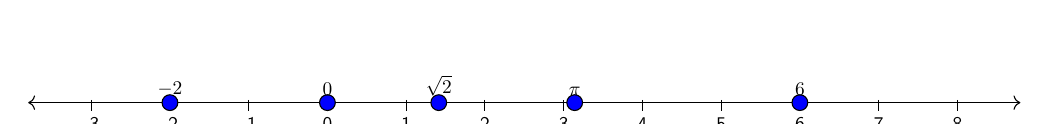
\begin{tikzpicture}[scale=1]
    \draw[<->] (-3.8,0) -- (8.8,0);
		\foreach \x in {-3,-2,-1,0,1,2,3,4,5,6,7,8} {\draw (\x,1pt) -- (\x,-3pt) node[anchor=north,scale=0.7] {\x};}
		\draw[fill=\blue]  (-2,0) circle (0.1); \node[above,scale=0.7] at (-2,0) {$-2$}; 
		\draw[fill=\blue]  (0,0) circle (0.1); \node[above,scale=0.7] at (0,0) {$0$}; 
		\draw[fill=\blue]  (1.414,0) circle (0.1); \node[above,scale=0.7] at (1.414,0) {$\sqrt{2}$}; 
		\draw[fill=\blue]  (3.14,0) circle (0.1); \node[above,scale=0.7] at (3.14,0) {$\pi$}; 
		\draw[fill=\blue]  (6,0) circle (0.1); \node[above,scale=0.7] at (6,0) {$6$}; 
    \end{tikzpicture}
\end{center}

Inequalities in real numbers translates to intervals along the real number line. For example:
\sitem{
\item The interval $-1 < x \leq 3$ translate too
\smallskip
\begin{center}
  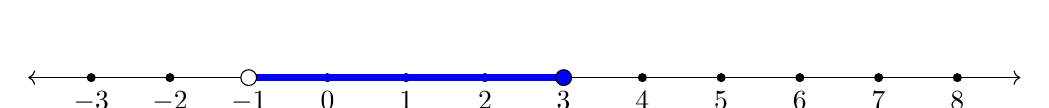
\begin{tikzpicture}[scale=1]
    \draw[<->] (-3.8,0) -- (8.8,0);
		\foreach \x in {-3,-2,-1,0,1,2,3,4,5,6,7,8} {\node[dot=1,label=below:$\x$] at  (\x, 0) {}; }
		\draw[line width=0.8mm, \blue] (-1,0) -- (3,0); 
		\draw[fill=white]  (-1,0) circle (0.1); %\node[above] at (-3,0) {$-3$}; 
		\draw[fill=\blue]  (3,0) circle (0.1); %\node[above] at (2,0) {$2$}; 
    \end{tikzpicture}
 \end{center}

\item The interval $1\leq x < 6$ translates to
\smallskip
\begin{center}
  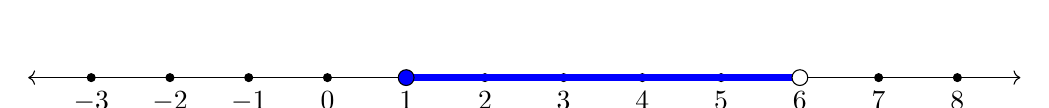
\begin{tikzpicture}[scale=1]
    \draw[<->] (-3.8,0) -- (8.8,0);
		\foreach \x in {-3,-2,-1,0,1,2,3,4,5,6,7,8} {\node[dot=1,label=below:$\x$] at  (\x, 0) {}; }
		\draw[line width=0.8mm,\blue] (1,0) -- (6,0); 
		\draw[fill=\blue]  (1,0) circle (0.1); %\node[above] at (2,0) {$2$}; 
		\draw[fill=white]  (6,0) circle (0.1); %\node[above] at (-3,0) {$-3$}; 
		\end{tikzpicture}
 \end{center}
}
\end{example}

We can extend this idea to complex numbers. Since two pieces of data is required to describe a complex number (a real part and an imaginary
part). We can use those two data as co-ordinates on the plane. The complex number $z = a+ib$ is represented by the point with co-ordinates $(a,b)$ in the plane. Complex numbers written in $z=a+ib$ is often called \emph{Cartesian form} for its connection with coordinates in the complex plane.

\begin{center}
\begin{tikzpicture}[scale=0.8]
	  \draw[<->] (-6.2,0) -- (6.2,0) ; \node[above] at (6.3,0) {$\RE{z}$};
    \draw[<->] (0,-4.2) -- (0,4.2) ; \node[right] at (0,4.3) {$\IM{z}$}; 
    	\foreach \x in {-6,-5,-4,-3,-2,-1,1,2,3,4,5,6}
     		\draw (\x,1pt) -- (\x,-3pt) node[anchor=north,scale=0.7] {\x};
    	\foreach \y in {-4,-3,-2,-1,1,2,3,4}
     		\draw (1pt,\y) -- (-3pt,\y) node[anchor=east,scale=0.7] {\y};
		\draw[fill=\blue]  (-5,3) circle (0.1) node[above] {$-5+3i$};
		\draw[fill=\blue]  (2,1) circle (0.1) node[above] {$2+i$};
		\draw[fill=\blue]  (-3,-3) circle (0.1) node[above] {$-3-3i$};
		\draw[fill=\blue]  (4,-2) circle (0.1) node[above] {$4-2i$};
\end{tikzpicture}
\end{center}

This is known as an \emph{Argand Diagram} or the \emph{complex plane}. The Argand diagram provides a simple visual way of representing many of the key properties of complex numbers.

\begin{example}
Let $z$ be a complex number. The Argand diagram of $\conj{z}$, the complex conjugate of $z$, is the point obtained by reflection in the real axis.
\begin{center}
\begin{tikzpicture}[scale=0.6]
	  \draw[<->] (-6.2,0) -- (6.2,0) ; \node[above,scale=0.7] at (6.3,0) {$\RE{z}$};
    \draw[<->] (0,-4.2) -- (0,4.2) ; \node[right,scale=0.7] at (0,4.3) {$\IM{z}$}; 
    	\foreach \x in {-6,-5,-4,-3,-2,-1,1,2,3,4,5,6}
     		\draw (\x,1pt) -- (\x,-3pt) node[anchor=north,scale=0.7] {\x};
    	\foreach \y in {-4,-3,-2,-1,1,2,3,4}
     		\draw (1pt,\y) -- (-3pt,\y) node[anchor=east,scale=0.7] {\y};
		\draw[fill=\blue]  (-5,3) circle (0.1) node[above] {$z$};
		\draw[fill=\blue]  (-5,-3) circle (0.1) node[above] {$\conj{z}$};
		\draw[fill=\blue]  (4,2) circle (0.1) node[above] {$\conj{w}$};
		\draw[fill=\blue]  (4,-2) circle (0.1) node[above] {$w$};
\end{tikzpicture}
\end{center}
\end{example}

\begin{exercise}{}
Plot all complex numbers of the form $z = a+3i$ for real numbers $a$
\end{exercise}
\begin{solution}

The imaginary part of $z$ is always 3 while the real part can vary. This leads to the following picture:

\begin{center}
\begin{tikzpicture}[scale=0.6]
	  \draw[<->] (-6.2,0) -- (6.2,0) ; \node[above,scale=0.7] at (6.3,0) {$\RE{z}$};
    \draw[<->] (0,-4.2) -- (0,4.2) ; \node[right,scale=0.7] at (0,4.3) {$\IM{z}$}; 
    	\foreach \x in {-6,-5,-4,-3,-2,-1,1,2,3,4,5,6}
     		\draw (\x,1pt) -- (\x,-3pt) node[anchor=north,scale=0.7] {\x};
    	\foreach \y in {-4,-3,-2,-1,1,2,4}
     		\draw (1pt,\y) -- (-3pt,\y) node[anchor=east,scale=0.7] {\y};
		\draw[<->, thick, \blue]  (-6,3) -- (6,3);
		\node[above,scale=0.7] at (4,3) {$z = a+3i$};
\end{tikzpicture}
\end{center}
\end{solution}

\begin{exercise}[label=ex:compcircle]{}
Plot all complex numbers $z = a+ib$ with the property that $a^2+b^2=9$.
\end{exercise}

\begin{solution}
Recall that $a^2+b^2=9$ is the equation of a circle with radius $3$. Thus a complex number $a+ib$ satisfies $a^2+b^2=9$ if it
lies on this circle.

\begin{center}
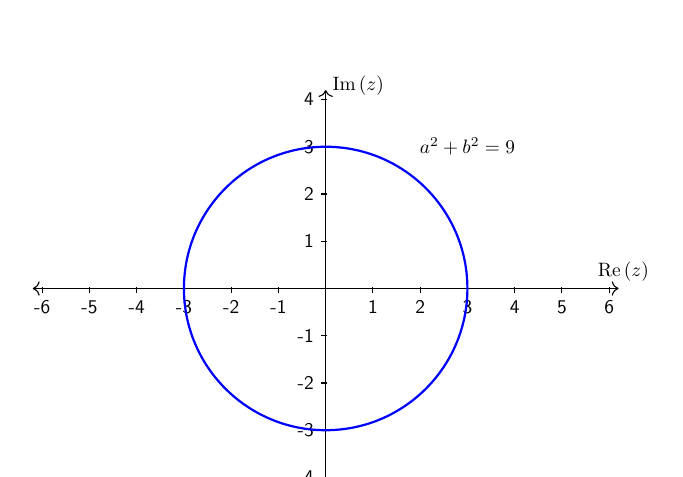
\begin{tikzpicture}[scale=0.6]
	  \draw[<->] (-6.2,0) -- (6.2,0) ; \node[above,scale=0.7] at (6.3,0) {$\RE{z}$};
    \draw[<->] (0,-4.2) -- (0,4.2) ; \node[right,scale=0.7] at (0,4.3) {$\IM{z}$}; 
    	\foreach \x in {-6,-5,-4,-3,-2,-1,1,2,3,4,5,6}
     		\draw (\x,1pt) -- (\x,-3pt) node[anchor=north,scale=0.7] {\x};
    	\foreach \y in {-4,-3,-2,-1,1,2,3,4}
     		\draw (1pt,\y) -- (-3pt,\y) node[anchor=east,scale=0.7] {\y};
		\draw[thick, \blue]  (0,0) circle (3);
		\node[scale=0.7] at (3,3) {$a^2+b^2=9$};
\end{tikzpicture}
\end{center}
Each point on the circle is a complex number satisfying the requirement.
\end{solution}

\begin{exercise}[label=ex:compcircle2]{}
Plot all complex numbers $z = a+ib$ with the property that 
$z \bar{z}=9$.
\end{exercise}

\begin{solution}
This is a retread of the previous question since $z \bar{z}= a^2+b^2=9$ is the equation of a circle with radius $3$. 

\begin{center}
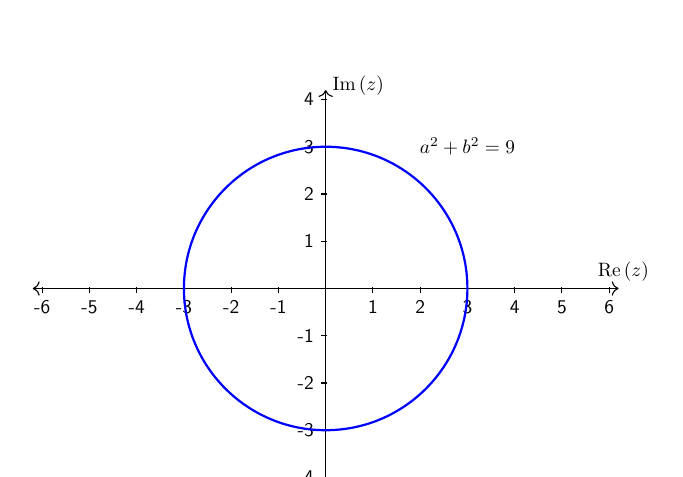
\begin{tikzpicture}[scale=0.6]
	  \draw[<->] (-6.2,0) -- (6.2,0) ; \node[above,scale=0.7] at (6.3,0) {$\RE{z}$};
    \draw[<->] (0,-4.2) -- (0,4.2) ; \node[right,scale=0.7] at (0,4.3) {$\IM{z}$}; 
    	\foreach \x in {-6,-5,-4,-3,-2,-1,1,2,3,4,5,6}
     		\draw (\x,1pt) -- (\x,-3pt) node[anchor=north,scale=0.7] {\x};
    	\foreach \y in {-4,-3,-2,-1,1,2,3,4}
     		\draw (1pt,\y) -- (-3pt,\y) node[anchor=east,scale=0.7] {\y};
		\draw[thick, \blue]  (0,0) circle (3);
		\node[scale=0.7] at (3,3) {$a^2+b^2=9$};
\end{tikzpicture}
\end{center}

\end{solution}

%\tutorial{sec:compargand}

\secbreak \subsection{Polar Form}

Now that we have a visual representation of complex numbers, we can ask new questions about them. For example, what is the \emph{size} of a complex number. One way to define size is to take the distance between the number and the origin of the Argand diagram\footnote{This idea of using distance to origin as size is consistent with our knowledge \emph{vectors}}. 
\begin{center}
\begin{tikzpicture}[scale=0.6]
	  \draw[->] (-0.2,0) -- (6.2,0) ; \node[above,scale=0.7] at (6.3,0) {$\RE{z}$};
    \draw[->] (0,-0.2) -- (0,4.2) ; \node[right,scale=0.7] at (0,4.3) {$\IM{z}$}; 
		\draw[fill=\blue]  (5,3) circle (0.1) node[above] {$z=a+ib$};
		\draw[\blue,->] (0,0) -- node[above left] {$r$} ++ (5,3);
\end{tikzpicture}
\end{center}
Using Pythagoras' Theorem we get
\begin{align*}
r^2&=a^2+b^2 &r&=\sqrt{a^2+b^2}
\end{align*}

\begin{df}{Modulus}
The \emph{modulus} of the complex number $z =a+ib$ is denoted $\abs{z} = \abs{a+ib}$ and is defined by
\begin{align*}
\abs{z} &= \abs{a+ib} = \sqrt{a^2+b^2}
\end{align*}
\end{df}

\begin{exercise}{}
If $z=3-i$ calculate $\abs{z}$.
\end{exercise}
\begin{solution}
Since $z=a+ib$ with $a=3$ and $b=-1$, we have
\begin{align*}
\abs{z} &=\sqrt{3^2+(-1)^2} =\sqrt{10}
\end{align*}
\end{solution}


\begin{exercise}{}
Find the modulus of the following complex numbers
\senum{
\item $z = i$
\item $z = -9$,
\item $z = \abs{\frac{1}{\sqrt{2}}- \frac{1}{\sqrt{2}}i}$
}
\end{exercise}
\begin{solution}
Applying the theorem, we have
\senum{
\item $\abs{i}=\sqrt{0^2+1^2}=1$
\item $\abs{-9}=\sqrt{9^2+0^2}=9$
\item $\displaystyle \abs{\frac{1}{\sqrt{2}}- \frac{1}{\sqrt{2}}i}= \sqrt{\frac{1}{2}+\frac{1}{2}}=1.$
}
\end{solution}

\begin{exercise}{}
In the Argand diagram, draw the set of all complex numbers $z$ with modulus $\abs{z} = \sqrt{2}$.
\end{exercise}
\begin{solution}
A complex number $z = a+ib$ has modulus $\abs{z} = \sqrt{2}$ if $\sqrt{a^2+b^2}=\sqrt{2}$ or $a^2+b^2=2$ (See \autoref{ex:compcircle}).
\end{solution}

\begin{solution}
(Alternate) We know that the modulus of a complex number gives the distance to the origin. Thus we want all the points at distance $\sqrt2$ from the origin. This again leads to the circle of radius $\sqrt2$ (See \autoref{ex:compcircle}). 
\end{solution}

\begin{exercise}[label=ex:compareas]{}
Plot the set of complex numbers $z$ satisfying $1 < |z| \leq 2$ in the complex plane.
\end{exercise}
\begin{solution}
Since the modulus is the distance to the origin the set consists of all those complex numbers which are at a distance between $1$ and $2$ from the origin. This
gives the area shown below.

\begin{center}
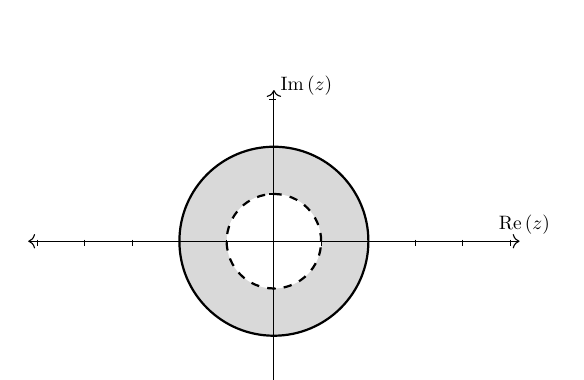
\begin{tikzpicture}[scale=0.6]
		\draw[fill=\gray, thick]  (0,0) circle (2);
		\draw[fill=\white, dashed, thick]  (0,0) circle (1);
	  \draw[<->] (-5.2,0) -- (5.2,0) ; \node[above,scale=0.7] at (5.3,0) {$\RE{z}$};
    \draw[<->] (0,-3.2) -- (0,3.2) ; \node[right,scale=0.7] at (0,3.3) {$\IM{z}$}; 
    	\foreach \x in {-5,-4,-3,-2,-1,1,2,3,4,5}
     		\draw (\x,1pt) -- (\x,-3pt);
    	\foreach \y in {-3,-2,-1,1,2,3}
     		\draw (1pt,\y) -- (-3pt,\y);
\end{tikzpicture}
\end{center}
\end{solution}
\caution Notice the difference between the inner and outer boundaries. A solid line indicates that the boundary is included and a dashed line indicates that the boundary is not included\footnote{This is analogous to using filled and hollowed circles to indicate endpoints of a real interval.}.

To uniquely define a complex number with the modulus, we would need another piece of information. This second piece of information is called the \emph{argument}.

\begin{df}[label=df:comparg]{(Principal) Argument}
Let $z$ be a complex number. The principal argument of $z$, denoted as $\Arg{z}$, is the angle $\theta$ in radians that $z$
makes with the positive real axis in a counter-clockwise direction, chosen so that $-\pi<\theta\leq\pi$.
\end{df}

A point $z$ in the Argand diagram determines an angle $\theta$ with the positive real axis.

\begin{center}
\begin{tikzpicture}[scale=0.8]
	  \draw[->] (-0.2,0) -- (6.2,0) ; \node[above,scale=0.7] at (6.3,0) {$\RE{z}$};
    \draw[->] (0,-0.2) -- (0,4.2) ; \node[right,scale=0.7] at (0,4.3) {$\IM{z}$}; 
		\draw[->] (0,0) -- (5,3);
		\draw[fill=\blue]  (5,3) circle (0.1) node[above] {$z$};
		\draw[\blue,->] (2,0) arc (0:31:2);
		\node[scale=0.7, \blue] at (2.2,0.5) {$\theta$};
\end{tikzpicture}
\end{center}

The choice of $\theta$ such that $-\pi<\theta\le\pi$ means:
\sitem{
\item $0 < \theta \leq \pi$ if $z$ is \emph{above} the real axis
\item $-\pi < \theta < 0$ if $z$ is \emph{below} the real axis
}

\begin{example}
The most straight forward method of determining the argument is to draw the diagram.

\begin{minipage}{0.5\textwidth}
\begin{center}
\begin{tikzpicture}[scale=0.4]
	  \draw[<->] (-6.2,0) -- (6.2,0) ; \node[above,scale=0.7] at (6.3,0) {$\RE{z}$};
    \draw[<->] (0,-4.2) -- (0,4.2) ; \node[right,scale=0.7] at (0,4.3) {$\IM{z}$}; 
		\draw[->,\blue] (0,0) -- (5,0);
		\draw[fill=\blue]  (5,0) circle (0.1) node[below] {$5$};
\end{tikzpicture}
\end{center}
\begin{center}
\begin{tikzpicture}[scale=0.4]
	  \draw[<->] (-6.2,0) -- (6.2,0) ; \node[above,scale=0.7] at (6.3,0) {$\RE{z}$};
    \draw[<->] (0,-4.2) -- (0,4.2) ; \node[right,scale=0.7] at (0,4.3) {$\IM{z}$}; 
		\draw[->,\blue] (0,0) -- (0,2);
		\draw[fill=\blue]  (0,2) circle (0.1) node[left] {$2i$};
		\draw[\blue,->] (1,0) arc (0:90:1);
\end{tikzpicture}
\end{center}

\end{minipage}%
\begin{minipage}{0.5\textwidth}
\begin{center}
\begin{tikzpicture}[scale=0.4]
	  \draw[<->] (-6.2,0) -- (6.2,0) ; \node[above,scale=0.7] at (6.3,0) {$\RE{z}$};
    \draw[<->] (0,-4.2) -- (0,4.2) ; \node[right,scale=0.7] at (0,4.3) {$\IM{z}$}; 
		\draw[->,\blue] (0,0) -- (-3,0);
		\draw[fill=\blue]  (-3,0) circle (0.1) node[below] {$3$};
		\draw[\blue,->] (1,0) arc (0:180:1);
\end{tikzpicture}
\end{center}
\begin{center}
\begin{tikzpicture}[scale=0.4]
	  \draw[<->] (-6.2,0) -- (6.2,0) ; \node[above,scale=0.7] at (6.3,0) {$\RE{z}$};
    \draw[<->] (0,-4.2) -- (0,4.2) ; \node[right,scale=0.7] at (0,4.3) {$\IM{z}$}; 
		\draw[->,\blue] (0,0) -- (0,-4);
		\draw[fill=\blue]  (0,-4) circle (0.1) node[left ] {$-4i$};
		\draw[\blue,->] (1,0) arc (0:-90:1);
\end{tikzpicture}
\end{center}
\end{minipage}

Based on the diagrams, we have:
\begin{align*}
\Arg{5}&=0 & \Arg{-3}&=\pi\\
\Arg{2i}&=\frac{\pi}{2} & \Arg{-4i}&=-\frac{\pi}{2}
\end{align*}

A similar approach would show that
\begin{align*}
\Arg{1+i} &=\frac{\pi}{4}&
\Arg{-1+i}&=\frac{3\pi}{4}\\
\Arg{1-i} &=-\frac{\pi}{4}&
\Arg{-1-i}&=-\frac{3\pi}{4}
\end{align*}
\end{example}



\begin{example}
We can use our knowledge of coordinate axes to determine:
\begin{align*}
\Arg{1} &=0&
\Arg{i}&=\frac{\pi}{2}\\
\Arg{-1} &=\pi&
\Arg{-i}&=-\frac{\pi}{2}
\end{align*}
Further, we can use the special triangles to get
\begin{align*}
\Arg{\sqrt{3}+i} &=\frac{\pi}{6}&
\Arg{1+i\sqrt{3}} &=\frac{\pi}{3}
\end{align*}
\end{example}

These are all cases we can obtain the angles by drawing and using our experience with simple triangles. We can extend this and develop a more systematic method to use for more general complex numbers

\begin{example}
Suppose $z=a+ib$ is a complex number which determines an angle $\theta$ with the real axis. 

\begin{center}
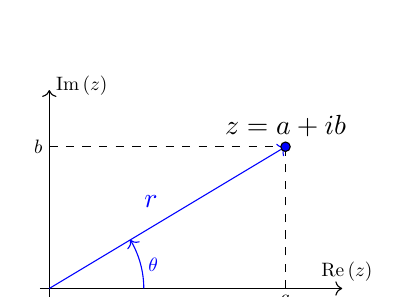
\begin{tikzpicture}[scale=0.6]
	  \draw[->] (-0.2,0) -- (6.2,0) ; \node[above,scale=0.7] at (6.3,0) {$\RE{z}$};
    \draw[->] (0,-0.2) -- (0,4.2) ; \node[right,scale=0.7] at (0,4.3) {$\IM{z}$}; 
		\draw[\blue,->] (0,0) -- node[above left] {$r$} ++ (5,3);
		\draw[dashed] (5,0) -- (5,3);
		\draw[dashed] (0,3) -- (5,3);
		\node[left,scale=0.7] at (0,3) {$b$}; 
		\node[below,scale=0.7] at (5,0) {$a$}; 
		\draw[fill=\blue]  (5,3) circle (0.1) node[above] {$z=a+ib$};
		\draw[\blue,->] (2,0) arc (0:31:2);
		\node[scale=0.7, \blue] at (2.2,0.5) {$\theta$};
\end{tikzpicture}
\end{center}


We can use our knowledge of trigonometry to get that
\begin{equation*}
\tan(\theta) = \frac{b}{a}
\end{equation*}
In order words, we can determine the argument $\theta$ from the Cartesian form. 
\end{example}

\caution In the case where $a=0$, we are on the imaginary axis and can resolve the angle using more simple methods.

\begin{exercise}{}
Find $\Arg{1+2i}$.
\end{exercise}

\begin{solution}
We start by plotting a diagram 

\begin{center}
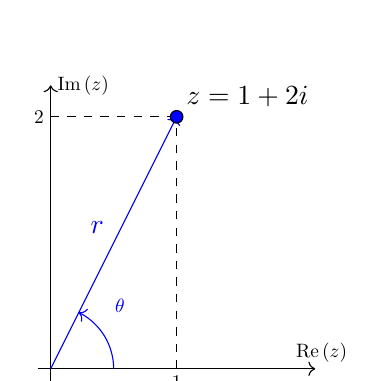
\begin{tikzpicture}[scale=0.8]
	  \draw[->] (-0.2,0) -- (4.2,0) ; \node[above,scale=0.7] at (4.3,0) {$\RE{z}$};
    \draw[->] (0,-0.2) -- (0,4.5) ; \node[right,scale=0.7] at (0,4.5) {$\IM{z}$}; 
		\draw[\blue,->] (0,0) -- node[above left] {$r$} ++ (2,4);
		\draw[dashed] (2,0) -- (2,4);
		\draw[dashed] (0,4) -- (2,4);
		\node[left,scale=0.7] at (0,4) {$2$}; 
		\node[below,scale=0.7] at (2,0) {$1$}; 
		\draw[fill=\blue]  (2,4) circle (0.1) node[above right] {$z=1+2i$};
		\draw[\blue,->] (1,0) arc (0:63.5:1);
		\node[scale=0.7, \blue] at (1.1,1) {$\theta$};
\end{tikzpicture}
\end{center}

Using the above formula we know that $\tan(\theta)=\frac{2}{1} = 2$. Using a calculator we get 
\begin{equation*}
\theta =\arctan(2) = 1.107
\end{equation*}
to 3 decimal places (in radians!).

\end{solution}
\caution Even though we have $\tan(\theta) = \frac{b}{a}$, we have cases where $\theta \neq \arctan\left(\frac{b}{a}\right)$.


\begin{example}
Suppose we want to find $\Arg{-1-2i}$ using the same method. We will that $\frac{b}{a}  = \frac{-2}{-1} =2$, which will give $\theta =\arctan(2) = 1.107$. However this is clearly not correct based on our previous exercise. That is $w=-1-2i$ and $z=1+2i$ are not in the same direction.

\end{example}

The reason for this is because the inverse tangent function produces values $-\frac{\pi}{2} < \theta < \frac{\pi}{2}$. In other words, the it assumes $a >0$. If we want to obtain the argument for the complex number in the exact opposite direction, we have to account for it by adding or subtracting $\pi$

\begin{example}
Consider the numbers $z = 1+i$ and $w = -1-i$. We know $\Arg{z} = \frac{\pi}{4}$ and $\Arg{w} = -\frac{3\pi}{4}$  and $\tan\left(\frac{\pi}{4}\right) = \tan\left(\frac{-3\pi}{4}\right)=1$. If we plot a diagram, we see why this is the case and how we can resolve it.

\begin{center}
\begin{tikzpicture}[scale=0.8]
	  \draw[->] (-4.2,0) -- (4.2,0) ; \node[above,scale=0.7] at (4.3,0) {$\RE{z}$};
    \draw[->] (0,-3.2) -- (0,3.5) ; \node[right,scale=0.7] at (0,3.5) {$\IM{z}$}; 
		\draw[\blue,->] (0,0) -- (2,2);
		\draw[\red ,->] (0,0) -- (-2,-2);
		\draw[\blue,->] (1,0) arc (0:45:1);
		\draw[\red ,->] (1,0) arc (0:-135:1);
		\draw[->] (0.5,0) arc (0:-135:0.5);
		\draw[->] (0.5,0) arc (0:45:0.5);
		\draw[fill=\blue]  (2,2) circle (0.1) node[above right] {$z$};
		\draw[fill=\red ]  (-2,-2) circle (0.1) node[below left] {$w$};
		\node[scale=0.7] at (0.5,-0.5) {$\pi$};
		\node[scale=0.7, \blue] at (1.1,0.5) {$\frac{\pi}{4}$};
		\node[scale=0.7, \red] at (-0.6,-1.3) {$\frac{-3\pi}{4}$};
\end{tikzpicture}
\end{center}

Be sure to have your calculator set to \textbf{radians} mode 
\end{example}

\begin{thm}[title= Summary \thethm\;]{}
To find $\theta =\Arg{a+ib}$, 
\begin{enumerate}
\item Draw a picture showing the angle. Stop if the angle is from a special triangle or on the axes.
\item Determine which {\it quadrant} the point is in and use the following:
\end{enumerate}
\begin{center}
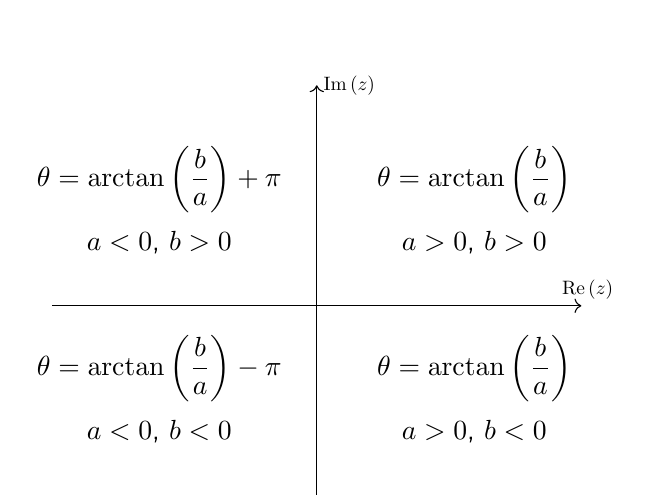
\begin{tikzpicture}[scale=0.8]
	  \draw[->] (-4.2,0) -- (4.2,0) ; \node[above,scale=0.7] at (4.3,0) {$\RE{z}$};
    \draw[->] (0,-3.2) -- (0,3.5) ; \node[right,scale=0.7] at (0,3.5) {$\IM{z}$}; 
		\node[scale=1] at (-2.5,2.0) {$\displaystyle \theta =\arctan\left(\frac{b}{a}\right)+\pi$};
		\node[scale=1] at (-2.5,1.0) {$a<0$, $b>0$};
		\node[scale=1] at (2.5,2.0) {$\displaystyle \theta =\arctan\left(\frac{b}{a}\right)$};
		\node[scale=1] at (2.5,1.0) {$a>0$, $b>0$};
		\node[scale=1] at (-2.5,-1.0) {$\displaystyle \theta =\arctan\left(\frac{b}{a}\right)-\pi$};
		\node[scale=1] at (-2.5,-2.0) {$a<0$, $b<0$};
		\node[scale=1] at (2.5,-1.0) {$\displaystyle \theta =\arctan\left(\frac{b}{a}\right)$};
		\node[scale=1] at (2.5,-2.0) {$a>0$, $b<0$};
\end{tikzpicture}
\end{center}

The four {\it quadrants} of the complex plane are usually numbered anti-clockwise.

% Four quadrants in the complex plane (Argand diagram), labelled I–IV.
% Style: clean axes with arrows, light quadrant shading, roman numerals.
\begin{center}
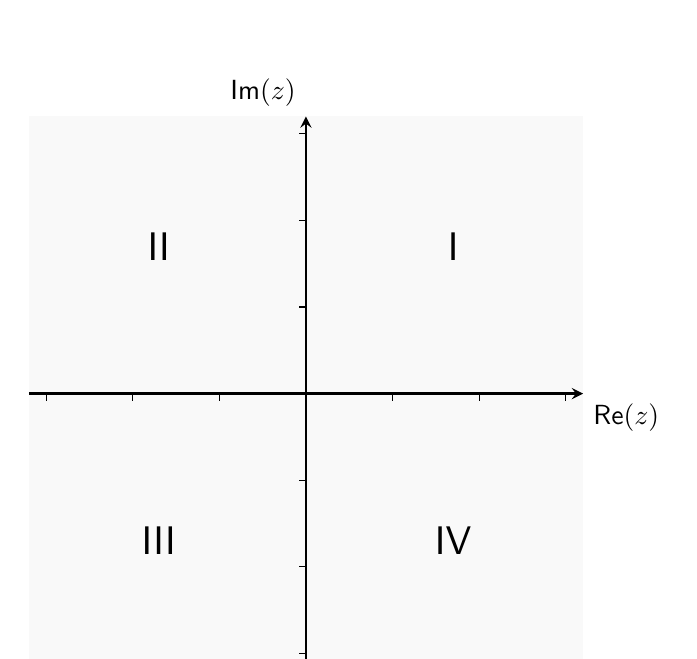
\begin{tikzpicture}[scale=1.1,>=stealth]
  % Axes limits
  \def\xmax{3.2}
  \def\ymax{3.2}

  % Light quadrant shading (optional; comment out if you prefer white)
  \fill[gray!05] (0,0) rectangle (\xmax,\ymax);      % QI
  \fill[gray!05] (-\xmax,0) rectangle (0,\ymax);     % QII
  \fill[gray!05] (-\xmax,-\ymax) rectangle (0,0);    % QIII
  \fill[gray!05] (0,-\ymax) rectangle (\xmax,0);     % QIV

  % Axes
  \draw[->,thick] (-\xmax,0) -- (\xmax,0) node[below right] {Re$(z)$};
  \draw[->,thick] (0,-\ymax) -- (0,\ymax) node[above left] {Im$(z)$};

  % Tick marks (minimal)
  \foreach \t in {-3,-2,-1,1,2,3}{
    \draw (\t,0) -- (\t,-0.08);
    \draw (0,\t) -- (-0.08,\t);
  }

  % Quadrant labels (roman numerals)
  \node at ( 1.7, 1.7) {\Large I};
  \node at (-1.7, 1.7) {\Large II};
  \node at (-1.7,-1.7) {\Large III};
  \node at ( 1.7,-1.7) {\Large IV};

  % Dashed lines for the axes (optional; uncomment if your notes use them)
  % \draw[dashed,gray] (-\xmax,0) -- (\xmax,0);
  % \draw[dashed,gray] (0,-\ymax) -- (0,\ymax);
\end{tikzpicture}
\end{center}




\end{thm}

\newpage
\begin{exercise}[label=ex:comparg]{}
Find $\Arg{-1+2i}$. 
\end{exercise}
\begin{solution}
Starting with the picture:

%\insf{another damned picture} - Kept original comment. -Tom
\begin{center}
\begin{tikzpicture}[scale=0.8]
	  \draw[->] (-2.2,0) -- (2.2,0) ; \node[above,scale=0.7] at (2.3,0) {$\RE{z}$};
    \draw[->] (0,-0.2) -- (0,3.5) ; \node[right,scale=0.7] at (0,3.5) {$\IM{z}$}; 
		\draw[\blue,->] (0,0) -- node[below left] {$r$} ++ (-1,2);
		\draw[fill=\blue]  (-1,2) circle (0.1) node[above left] {$z=-1+2i$};
		\draw[\blue,->] (0.5,0) arc (0:116.5:0.5);
		\node[scale=0.7, \blue] at (0.5,0.5) {$\theta$};
\end{tikzpicture}
\end{center}
We see that $0<\Arg{-1+2i} <\pi$. Using the above formula we know that $\tan(\theta)=\frac{2}{-1}=-2$. Using a calculator we get
\begin{equation*}
\arctan(-2)=-1.107
\end{equation*}
to 3 decimal places. Since this is not in the correct range for $\theta$. Adding $\pi$ gives
\begin{equation*}
\theta = -1.107+\pi = 2.034
\end{equation*}

\end{solution}



\begin{exercise}{}
Find $\Arg{3-4i}$.
\end{exercise}
\begin{solution}
We see that $-\frac{\pi}{2}<\Arg{3-4i}<0$, so the inverse tangent value should give us the right argument. This gives:
\begin{equation*}
\Arg{3-4i}=\arctan\left(\frac{-4}{3}\right)= -0.927.
\end{equation*}
\end{solution}

Now that we have we can determine the modulus and argument of a complex number, we can try to reverse the process.

\begin{df}{Polar form}
Let $z$ be a complex number with modulus $r$ and principal argument $\theta$. The polar form of $z$ is given by
\begin{align*}
z &= r\cos(\theta) + i r\sin(\theta)\\
&= r\left(\cos(\theta) + i\sin(\theta)\right)
\end{align*}
\end{df}

We can verify this by looking at the picture and applying a bit of trigonometry.
\begin{center}
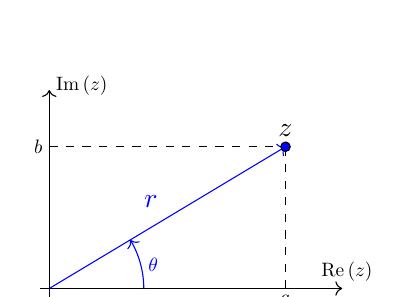
\begin{tikzpicture}[scale=0.6]
	  \draw[->] (-0.2,0) -- (6.2,0) ; \node[above,scale=0.7] at (6.3,0) {$\RE{z}$};
    \draw[->] (0,-0.2) -- (0,4.2) ; \node[right,scale=0.7] at (0,4.3) {$\IM{z}$}; 
		\draw[\blue,->] (0,0) -- node[above left] {$r$} ++ (5,3);
		\draw[dashed] (5,0) -- (5,3);
		\draw[dashed] (0,3) -- (5,3);
		\node[left,scale=0.7] at (0,3) {$b$}; 
		\node[below,scale=0.7] at (5,0) {$a$}; 
		\draw[fill=\blue]  (5,3) circle (0.1) node[above] {$z$};
		\draw[\blue,->] (2,0) arc (0:31:2);
		\node[scale=0.7, \blue] at (2.2,0.5) {$\theta$};
\end{tikzpicture}
\end{center}

From the picture, we see that the base $a = r\cos(\theta)$ and height $b = r\sin(\theta)$. Hence, we have
\begin{equation*}
z =r\cos(\theta)+i r\sin(\theta)
\end{equation*}

\begin{exercise}{}
Suppose $\abs{z}=2$ and $\Arg{z}=\frac{\pi}{3}$. Write $z$ in polar form.
\end{exercise}
\begin{solution}
Set $r=\abs{z}=2$ and $\theta=\Arg{z}=\frac{\pi}{3}$. Then
\begin{align*}
z&= r\left(\cos(\theta)+i\sin(\theta)\right)\\
 &= 2\left(\cos\left(\frac{\pi}{3}\right)+i\sin\left(\frac{\pi}{3}\right)\right)
\end{align*}
\end{solution}
If we wished to convert it to Cartesian form, we can further simplify
\begin{align*}
z&= 2\left(\cos\left(\frac{\pi}{3}\right)+i\sin\left(\frac{\pi}{3}\right)\right)\\
 &= 2\left(\frac{1}{2}+i\frac{\sqrt{3}}{2}\right)\\
 &= 1+i\sqrt{3}
\end{align*}

In general, if we want to write a complex number in polar form, we:
\begin{enumerate}
\item Compute the modulus, $r=\abs{z}$.
\item Computer the principal argument, $\theta=\Arg{z}$.
\item Write $z$ as
\begin{equation*}
z= r\left(\cos(\theta)+i\sin(\theta)\right)\\
\end{equation*}
\end{enumerate}

We will see in the next subsection that we can also write this as $z = r\, e^{i\theta}$.

\begin{exercise}[label=ex:1ipolar]{}
Write $z= 1+i$ in polar form.
\end{exercise}
\begin{solution}
First we calculate the modulus and principal argument.
\sitem{
\item Modulus: $\abs{z}=\sqrt{1^2+1^2}=\sqrt{2}$.
\item Principal Argument: $\Arg{z}=\arctan\left(\frac{1}{1}\right) = \frac{\pi}{4}$. Since $z$ is in the first quadrant, the argument does not need altering. 
}
Thus the polar form of $z= 1+i$ is
\begin{equation*}
z = \sqrt{2} \left(\cos\left(\frac{\pi}{4}\right)+i\sin\left(\frac{\pi}{4}\right)\right)
\end{equation*}
\end{solution}

\begin{exercise}{}
Write $z=-1+2i$ in polar form.
\end{exercise}
\begin{solution}
First we calculate the modulus and principal argument.
\sitem{
\item Modulus: $\abs{z}=\sqrt{(-1)^2+2^2}=\sqrt{5}$.
\item Principal Argument: $\Arg{z}=\arctan\left(\frac{2}{-1}\right) = -1.107$. Since $z$ is in the upper-left quadrant, we need to alter the argument (see \autoref{ex:comparg}) to get $\Arg{z} = 2.034$
}
Thus the polar form of $z= -1+2i$ is
\begin{equation*}
z = \sqrt{5} \left(\cos\left(2.034\right)+i\sin\left(2.034\right)\right)
\end{equation*}
\end{solution}

%\tutorial{sec:comppolar}

\secbreak \subsection{Exponential Form} 

The introduction of complex numbers connects two key areas of mathematics: Trigonometry and the exponential. It is possible to write a Maclaurin series for the exponential
\begin{equation*}
e^x = 1+x+\frac{x^2}{2!}+\frac{x^3}{3!} + \cdots = \sum_{n=0}^{\infty} \frac{x^n}{n!}
\end{equation*}

As it turns out, the exponential can be extended to complex numbers in the analogous way.

\begin{df}{Complex exponential}
For a complex number $z$, the complex exponential is defined to be:
\begin{equation*}
e^z = 1+z+\frac{z^2}{2!}+\frac{z^3}{3!} + \cdots = \sum_{n=0}^{\infty} \frac{z^n}{n!}
\end{equation*}
\end{df}

It is not at all obvious, but it is a fact that the infinite summation results in something finite for all complex $z$ so long as $|z|<\infty$.

If we consider the complex number $z=i\theta$ for an angle $\theta$, we get:
\begin{align*}
e^{i\theta} &= 1+\left(i\theta\right)+\frac{\left(i\theta\right)^2}{2!}+\frac{\left(i\theta\right)^3}{3!} + \cdots = \sum_{n=0}^{\infty} \frac{\left(i\theta\right)^n}{n!}
\end{align*}
By resolving the powers of $i$, we get
\begin{align*}
e^{i\theta} &= 1+\left(i\theta\right)+\frac{\left(i\theta\right)^2}{2!}+\frac{\left(i\theta\right)^3}{3!} + \frac{\left(i\theta\right)^4}{4!} + \frac{\left(i\theta\right)^5}{5!} + \cdots \\
&= 1+i\theta - \frac{\theta^2}{2!} -\frac{i\theta^3}{3!} + \frac{\theta^4}{4!} + \frac{i\theta^5}{5!} + \cdots\\
&= \left(1- \frac{\theta^2}{2!} + \frac{\theta^4}{4!} + \cdots \right) + i \left(\theta - \frac{\theta^3}{3!} + \frac{\theta^5}{5!} + \cdots\right)
\end{align*}
Recalling the Maclaurin series for $\sin(x)$ and $\cos(x)$ , we see that the two summations give:
\begin{align*}
e^{i\theta} &= \cos(\theta) + i \sin(\theta)
\end{align*}

This gives a fundamental result in complex numbers

\begin{thm}{Euler's Formula}
For any angle $\theta$, we have 
\begin{equation*}
e^{i\theta} = \cos(\theta) + i \sin(\theta)
\end{equation*}
\end{thm}

In particular, if $\theta =\pi$, we have the famous equation\footnote{This remarkable formula was obtained by Leonhard Euler in around 1768. The special case (one of the Top 10 equations ever!) links 5 fundamentally important numbers: $1$,$0$, $e$, $\pi$ and $i$ that have their origin in different branches of mathematics.}
\begin{equation*}
e^{i\pi} +1 = 0
\end{equation*}

\begin{example}
With Euler's formula, we have
\begin{align*}
e^{i1} &= \cos(1)+i\sin(1).\\
e^{i\frac{\pi}{2}} &= \cos\left(\frac{\pi}{2}\right)+i\sin\left(\frac{\pi}{2}\right) = 0 + 1i = i.
\end{align*}
\end{example}

Using Euler's formula we can get a new and very useful representation for complex numbers in polar form.

\begin{df}{Exponential form}
The exponential form of the complex number $z$ with modulus $r$ and argument $\theta$ is written as
\begin{equation*}
z = re^{i\theta}
\end{equation*}
\end{df}

We derive this form by applying Euler's Formula to the polar form
\begin{equation*}
z= r\left(\cos(\theta)+i\sin(\theta)\right) = re^{i\theta}
\end{equation*}

To write a complex number $z$ in exponential form:
\begin{enumerate}
\item Calculate the modulus $r = \abs{z}$,
\item Calculate the principle argument $\theta = \Arg{z}$,
\item Write $z=re^{i\theta}$.
\end{enumerate}


\begin{exercise}{}
Write $z = 1+i$ in exponential form.
\end{exercise}
\begin{solution}
Building on \autoref{ex:1ipolar}, we know $\abs{z}= \sqrt{2}$ and $\Arg{z}=\frac{\pi}{4}$.
Hence, the exponential form is
\begin{equation*}
z = 1+i= \sqrt2 e^{i\frac{\pi}{4}}.
\end{equation*}
\end{solution}

\begin{exercise}{}
\question Write $-i$ and $-1$ in exponential form.
\end{exercise}

Now that we have shown how to convert a complex number from Cartesian form $a+ib$ to exponential form $r e^{i\theta}$, we can go in the reverse direction.

\begin{exercise}{}
Write the complex number $z=2e^{i\frac{\pi}{4}}$ in Cartesian form $a+ib$.
\end{exercise}

\begin{solution}
Using Euler's formula, we have
\begin{align*}
z &= 2e^{i\frac{\pi}{4}}\\
&=2\left(\cos\left(\frac{\pi}{4}\right)+i\sin\left(\frac{\pi}{4}\right)\right) \\
&=2\left(\frac{1}{\sqrt{2}}+i\frac{1}{\sqrt{2}}\right)\\
&=\sqrt{2}+i \sqrt{2}
\end{align*}
\end{solution}

\begin{exercise}{}
Let $z=5+4i$. Write $e^z$ in the form $a+ib$.
\end{exercise}

\begin{solution}
We have (to 2 decimal point)
\begin{align*}
e^{5+4i} &= e^5e^{4i}\\
&= e^5\left(\cos(4)+i\sin(4)\right)\\
&=e^5\cos(4)+ie^5\sin(4)\\
&\approx -97.01-112.32i
\end{align*}
\end{solution}

Recall that multiplication and division of complex numbers can be quite an involved process (See \autoref{ex:compdiv}). However, we can utilise properties of the exponential function (and hence the exponential form) help simplify this process.

Let $z$ and $w$ be complex numbers. Then we have:
\begin{align*}
e^z\cdot e^w&=e^{z+w}  & \frac{e^z}{e^w} &=e^{z-w}  
\end{align*}

We can express this as:

\begin{thm}[label=thm:compmult]{Multiplication and division in exponential form}
Let $z = re^{i\theta}$ and $w = se^{i\phi}$ be complex numbers in exponential form
\begin{align*}
z\cdot w &= (r\cdot s) e^{i(\theta+\phi)} & \frac{z}{w} &= \frac{r}{s} e^{i(\theta-\phi)}.
\end{align*}
Converting the right-hand side to \emph{polar form} gives:
\begin{align*}
z\cdot w &= (r\cdot s) \left(\cos(\theta+\phi) + i \sin(\theta+\phi)\right) \\
\frac{z}{w} &= \frac{r}{s} \left(\cos(\theta-\phi) + i \sin(\theta-\phi)\right).
\end{align*}
\end{thm}

\begin{exercise}{}
Let $z=2e^{\frac{i \pi}{4}}$, and $w=e^{-\frac{i \pi}{4}}$. Find $z\cdot w$ and $\frac{z}{w}$.
\end{exercise}
\begin{solution}
Reading off the complex numbers, we get $r=2, s=1, \theta=\frac{\pi}{4}, \phi=-\frac{\pi}{4}$. So we get:
\begin{align*}
z\cdot w &= (2\cdot 1) \left[\cos\left(\frac{\pi}{4}+\left(-\frac{\pi}{4}\right)\right) + i \sin\left(\frac{\pi}{4}+\left(-\frac{\pi}{4}\right)\right)\right]\\
&=2\left[\cos(0)+i \sin(0)\right]=2\\
\frac{z}{w} &= \frac{2}{1} \left[\cos\left(\frac{\pi}{4}-\left(-\frac{\pi}{4}\right)\right) + i \sin\left(\frac{\pi}{4}-\left(-\frac{\pi}{4}\right)\right)\right]\\
&= \frac{2}{1} \left[\cos(\pi/2) + i \sin(\pi/2)\right] = 2i.
\end{align*}
\end{solution}

Complex exponentials are extremely useful when dealing with multiplication and division\footnote{but not so effective when dealing with addition and subtraction.}. However, its usefulness extends beyond simple arithmetic. For the rest of this section, we will take a (very brief) look into areas where complex exponentials might be useful.

\subsubsection*{Complex exponentials and trigonometric functions}

Euler's formula gives us an alternative way to write the sine and cosine functions which is used very widely in science and engineering. In particular, we have
\begin{align*}
e^{i\theta} + e^{-i\theta}  &= \left(\cos(\theta) + i \sin(\theta)\right) + \left(\cos(\theta) - i \sin(\theta)\right) = 2 \cos(\theta)\\
e^{i\theta} - e^{-i\theta}  &= \cos(\theta) + i \sin(\theta) - \left(\cos(\theta) - i \sin(\theta)\right) = 2 i \sin(\theta)
\end{align*}

We can rearrange to get the following:
\begin{thm}{Trigonometric functions in exponential forms}
We can express the trigonometric functions:
\begin{align*}
\cos(\theta) &= \frac{1}{2}\left(e^{i\theta} + e^{-i\theta}\right),\\
\sin(\theta) &= \frac{1}{2i}\left(e^{i\theta} - e^{-i\theta}\right).
\end{align*}
\end{thm}

Notice that these relations are very similar to the ones for the hyperbolic trigonometric functions (cosh and sinh). The introduction of complex numbers illustrates why they share so many similar identities.

\begin{exercise}{}
\question Use complex exponentials to show that $2\sin(\theta)\cos(\theta)=\sin(2\theta)$.
\end{exercise}

\subsubsection*{Calculus with complex exponentials}

The complex exponential is also commonly involved in the solution of differential equations, particularly in cases where solutions oscillate (like in AC electronics, quantum mechanics, etc.). It satisfies the same rules of differentiation and integration as any other exponential function\footnote{In essence, we can treat the complex number $i$ like a constant.}.

\begin{example}
For derivatives involving $i$, we have
\begin{align*}
\frac{d}{dx} e^{i \omega x} &= i \omega e^{i \omega x} \\
\frac{d^2}{dx^2} e^{i \omega x} &= (i \omega)^2 e^{i \omega x} = -\omega^2 e^{i \omega x}
\end{align*}
Integration works in a similar way
\begin{align*}
\int e^{i \omega x} dx &= \frac{e^{i \omega x}}{i\omega} + C
\end{align*}
\end{example}

\begin{exercise}{}
\question Verify that $y(t) = C e^{-i4t}$ is a solution of $y'' = -16 y$.
\end{exercise}

\subsubsection*{Logarithms of complex numbers}

Now that we have seen the exponential in complex numbers, it is natural to question how logarithm behave in complex numbers? The short answer is that logarithms are very complicated beasts, with properties far beyond this introductory course. \caution Use with caution! 

Suppose we ``naively'' apply logarithms on complex numbers using the rules of real numbers, we have the following.

\begin{example}
Let $z = r e^{i\theta}$ be a complex number in exponential form. We can apply the logarithm as
\begin{align*}
\Log(z) &= \Log\left(r e^{i\theta}\right)\\
&= \Log\left(r\right) + \Log\left(e^{i\theta}\right)\\
&= \Log\left(r\right) + i\theta\\
&= \Log\abs{z} + i\Arg{z}
\end{align*}
\end{example}

\begin{exercise}{}
Let $z = 42 e^{i\frac{\pi}{7}}$. Find $\Log(z)$.
\end{exercise}
\begin{solution}
Since $|z| = 42$ and $\Arg{z} = \frac{\pi}{7}$, we have $\Log(z) = \Log(42) + i\frac{\pi}{7}$.
\end{solution}

\caution Whilst this approach is not wrong, it also does not capture the entire picture\footnote{Recall from \autoref{df:comparg} that we have $-\pi < \Arg{z} \leq \pi$. However, this is a choice we made and there are other (non-principal) arguments we can take to be the angle of a complex number. For example, we could have chosen $0 < \Arg{z} \leq 2\pi$, which would affect the resulting logarithm.}.

%\tutorial{sec:compexponential}

\secbreak \subsection{De Moivre's Theorem}

Through repeated application of \autoref{thm:compmult}, we can extend exponential multiplication to powers of exponentials. We start with
\begin{equation*}
e^{i\theta} \cdot e^{i\theta} = e^{i (\theta+\theta)} = e^{i 2\theta}
\end{equation*}
which can be extended to any integer $n$ giving
\begin{equation*}
\left(e^{i\theta}\right)^n = e^{i n\theta}
\end{equation*}

If we convert both sides of the above equation into polar form, we obtain a very important result.

\begin{thm}{De Moivre's Theorem}
Let $n$ be an integer. For an angle $\theta$, we have
\begin{equation*}
\left(\cos(\theta)+i\sin(\theta)\right)^n = \cos(n\theta) +i\sin(n\theta).
\end{equation*}
For a complex number $z = r e^{i\theta}$ in exponential form, the following are equivalent
\begin{align*}
z^n &=  r^n e^{i n\theta} = r^n \left(\cos(n\theta) + i \sin(n\theta)\right)\\
&=  r^n \left(e^{i\theta}\right)^n = r^n \left(\cos(\theta)+i\sin(\theta)\right)^n
\end{align*}
\end{thm}

De Moivre's Theorem is particularly useful when dealing with powers of complex numbers. 

\begin{exercise}{}
Let $z=(1+i)$ and compute $z^8$
\end{exercise}

\begin{solution}
We first write $z$ in expontial form as
\begin{equation*}
z = 1+i=\sqrt{2} \left(\cos\left(\frac{\pi}{4}\right)+i\sin\left(\frac{\pi}{4}\right)\right) = \sqrt{2}e^{i\frac{\pi}{4}}
\end{equation*}
This gives
\begin{align*}
z^8 &= (1+i)^8\\
& = \left(\sqrt{2}e^{i\frac{\pi}{4}}\right)^8\\
& = \sqrt{2}^8 e^{i\frac{8\pi}{4}}\\
&= 16 e^{i2\pi}=16
\end{align*}
\end{solution}

We can reach the same solution by multiplying 8 times. But this would be rather tedious and not recommended.

\begin{exercise}{}
Compute $(-1+2i)^{10}$
\end{exercise}
\begin{solution}
Putting $z= (-1+2i)$ in exponential form, we find
\begin{equation*}
z= (-1+2i)=\sqrt{5}\big(\cos(2.034)+i \sin(2.034)\big) = \sqrt{5}e^{2.034i}
\end{equation*}
Thus we have
\begin{equation*}
z^{10} = (-1+2i)^{10} = \left(\sqrt{5}e^{2.034i}\right)^{10} = 3125 e^{20.34i} = 250.8+ 3115i
\end{equation*}
\end{solution}

De Moivre's theorem is also useful for computing roots of complex numbers.

\begin{thm}[label=thm:comproot]{Roots of complex numbers}
Let $z = r\, e^{i\theta}$ be a complex number in exponential form and $n$ be a positive integer. There are precisely $n$ different $n$-th roots of $z$ and they are given by
\begin{align*}
        z^{\frac{1}{n}} &= r^{\frac{1}{n}} e^{i \frac{\theta + 2\pi k}{n}}  &\text{for\;} k=0,1,\ldots,n-1
\end{align*}
where $r^{\frac{1}{n}}$ is the positive $n$-th root of $r$.
\end{thm}

\begin{example}
For \emph{square roots} of $z = re^{i\theta}$ we have $n=2$. So the \emph{two roots} $w_1, w_2$ are given by
\begin{align*}
w_1 &= \sqrt{r} e^{i\frac{\theta + 2\pi 0}{2}} = \sqrt{r} e^{i\frac{\theta}{2}}\\
w_2 &= \sqrt{r} e^{i\frac{\theta + 2\pi 1}{2}} = \sqrt{r} e^{i\frac{\theta + 2\pi}{2}}
\end{align*}
and $\sqrt{r}$ is the positive square root of $r$.

For \emph{cube roots} of $z = re^{i\theta}$ we have $n=3$. So the \emph{three roots} $w_1, w_2, w_3$ are given by
\begin{align*}
w_1 &= \sqrt[3]{r} e^{i\frac{\theta + 2\pi 0}{3}} = \sqrt[3]{r} e^{i\frac{\theta}{3}}\\
w_2 &= \sqrt[3]{r} e^{i\frac{\theta + 2\pi 1}{3}} = \sqrt[3]{r} e^{i\frac{\theta + 2\pi}{3}}
w_3 &= \sqrt[3]{r} e^{i\frac{\theta + 2\pi 2}{3}} = \sqrt[3]{r} e^{i\frac{\theta + 4\pi}{3}}
\end{align*}
and $\sqrt[3]{r}$ is the positive cubed root of $r$.
\end{example}


\begin{exercise}{}
Let $z = 9e^{i\frac{\pi}{3}}$. Find the two values of $\sqrt{z}$ and verify your answer.
\end{exercise}
\begin{solution}
Apply \autoref{thm:comproot} with $r=9$, $\theta = \frac{\pi}{3}$ and $n=2$ gives
\begin{align*}
w_1 &= \sqrt{9} e^{i\frac{\frac{\pi}{3} + 2\pi 0}{2}} \\
		&= 3 e^{i\frac{\pi}{6}} \\
w_2 &= \sqrt{9} e^{i\frac{\frac{\pi}{3} + 2\pi}{2}} \\
		&= 3 e^{i\frac{7\pi}{6}}
\end{align*}
We can verify the solutions by squaring the answer
\begin{align*}
(w_1)^2 &= \left(3 e^{i\frac{\pi}{6}}\right)^2 \\
				&= 9 e^{2i\frac{\pi}{6}} \\
				&= 9 e^{i\frac{\pi}{3}}\\
				&= z \\
(w_2)^2 &= \left(3 e^{i\frac{7\pi}{6}}\right)^2 \\
				&= 9 e^{2i\frac{7\pi}{6}} \\
				&= 9 e^{i\frac{14\pi}{6}} \\
				&= 9 e^{i\frac{2\pi}{6}}e^{i2\pi} \\
				&= z \cdot 1 = z
\end{align*}
\end{solution}


\begin{exercise}{}
\question Find the $5$-th roots of $z = -1 + 2i$. Confirm your answers by plotting it on the complex plane. 
\end{exercise}

\newpage

\begin{example}
Plotting the $n$-th roots of a complex number $z$ gives some interesting patterns.

\begin{multicols}{2}
\begin{center}
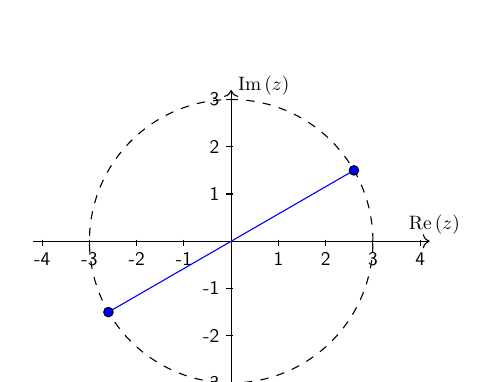
\begin{tikzpicture}[scale=0.6]
	  \draw[->] (-4.2,0) -- (4.2,0) ; \node[above,scale=0.7] at (4.3,0) {$\RE{z}$};
    \draw[->] (0,-3.2) -- (0,3.2) ; \node[right,scale=0.7] at (0,3.3) {$\IM{z}$}; 
		\foreach \x in {-4,-3,-2,-1,1,2,3,4}
     		\draw (\x,1pt) -- (\x,-3pt) node[anchor=north,scale=0.7] {\x};
    \foreach \y in {-3,-2,-1,1,2,3}
     		\draw (1pt,\y) -- (-3pt,\y) node[anchor=east,scale=0.7] {\y};
		\def\r{3}
		\def\theta{pi/3}
		\def\n{2}
		\draw[dashed] (0,0) circle (\r);
		\foreach \ii in {0,1}{
		\draw[\blue] (0,0) -- ({\r*cos(((\theta+2*pi*\ii)/\n) r)},{\r*sin(((\theta+2*pi*\ii)/\n) r)});
		\draw[fill=\blue]  ({\r*cos(((\theta+2*pi*\ii)/\n) r)},{\r*sin(((\theta+2*pi*\ii)/\n) r)}) circle (0.1);
		}
\end{tikzpicture}
\captionof{figure}{Square roots of $z= 9 e^{i\frac{\pi}{3}}$}
\end{center}

\begin{center}
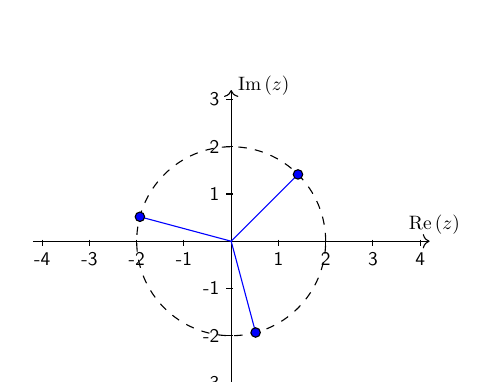
\begin{tikzpicture}[scale=0.6]
	  \draw[->] (-4.2,0) -- (4.2,0) ; \node[above,scale=0.7] at (4.3,0) {$\RE{z}$};
    \draw[->] (0,-3.2) -- (0,3.2) ; \node[right,scale=0.7] at (0,3.3) {$\IM{z}$}; 
		\foreach \x in {-4,-3,-2,-1,1,2,3,4}
     		\draw (\x,1pt) -- (\x,-3pt) node[anchor=north,scale=0.7] {\x};
    \foreach \y in {-3,-2,-1,1,2,3}
     		\draw (1pt,\y) -- (-3pt,\y) node[anchor=east,scale=0.7] {\y};
		\def\r{2}
		\def\theta{3*pi/4}
		\def\n{3}
		\draw[dashed] (0,0) circle (\r);
		\foreach \ii in {0,1,2}{
		\draw[\blue] (0,0) -- ({\r*cos(((\theta+2*pi*\ii)/\n) r)},{\r*sin(((\theta+2*pi*\ii)/\n) r)});
		\draw[fill=\blue]  ({\r*cos(((\theta+2*pi*\ii)/\n) r)},{\r*sin(((\theta+2*pi*\ii)/\n) r)}) circle (0.1);
		}
\end{tikzpicture}
\captionof{figure}{Third roots of $z= \frac{8(-1+i)}{\sqrt{2}}$}
\end{center}

\begin{center}
\begin{tikzpicture}[scale=0.6]
	  \draw[->] (-4.2,0) -- (4.2,0) ; \node[above,scale=0.7] at (4.3,0) {$\RE{z}$};
    \draw[->] (0,-3.2) -- (0,3.2) ; \node[right,scale=0.7] at (0,3.3) {$\IM{z}$}; 
		\foreach \x in {-4,-3,-2,-1,1,2,3,4}
     		\draw (\x,1pt) -- (\x,-3pt) node[anchor=north,scale=0.7] {\x};
    \foreach \y in {-3,-2,-1,1,2,3}
     		\draw (1pt,\y) -- (-3pt,\y) node[anchor=east,scale=0.7] {\y};
		\def\r{1.222844545}
		\def\theta{2.034443936}
		\def\n{4}
		\draw[dashed] (0,0) circle (\r);
		\foreach \ii in {0,1,2,3}{
		\draw[\blue] (0,0) -- ({\r*cos(((\theta+2*pi*\ii)/\n) r)},{\r*sin(((\theta+2*pi*\ii)/\n) r)});
		\draw[fill=\blue]  ({\r*cos(((\theta+2*pi*\ii)/\n) r)},{\r*sin(((\theta+2*pi*\ii)/\n) r)}) circle (0.1);
		}
\end{tikzpicture}
\captionof{figure}{$4$-th roots of $z= -1+2i$}
\end{center}

\begin{center}
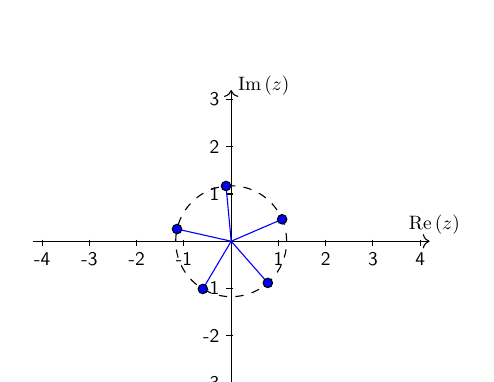
\begin{tikzpicture}[scale=0.6]
	  \draw[->] (-4.2,0) -- (4.2,0) ; \node[above,scale=0.7] at (4.3,0) {$\RE{z}$};
    \draw[->] (0,-3.2) -- (0,3.2) ; \node[right,scale=0.7] at (0,3.3) {$\IM{z}$}; 
		\foreach \x in {-4,-3,-2,-1,1,2,3,4}
     		\draw (\x,1pt) -- (\x,-3pt) node[anchor=north,scale=0.7] {\x};
    \foreach \y in {-3,-2,-1,1,2,3}
     		\draw (1pt,\y) -- (-3pt,\y) node[anchor=east,scale=0.7] {\y};
		\def\r{1.174618943}
		\def\theta{2.034443936}
		\def\n{5}
		\draw[dashed] (0,0) circle (\r);
		\foreach \ii in {0,1,2,3,4}{
		\draw[\blue] (0,0) -- ({\r*cos(((\theta+2*pi*\ii)/\n) r)},{\r*sin(((\theta+2*pi*\ii)/\n) r)});
		\draw[fill=\blue]  ({\r*cos(((\theta+2*pi*\ii)/\n) r)},{\r*sin(((\theta+2*pi*\ii)/\n) r)}) circle (0.1);
		}
\end{tikzpicture}
\captionof{figure}{$5$-th roots of $z= -1+2i$}
\end{center}
\end{multicols}
The $n$-th roots of $z = r e^{i\theta}$ are spaced equally in wedges with angle $\frac{2\pi}{n}$ around a circle of radius $r^{\frac{1}{n}}$. 
\end{example}


As a final application of De Moivre's theorem, we can use it to derive some useful trigonometric identities. 


\begin{example}
Consider the case of $n=2$ in De Moivre's Theorem. We get
\begin{align*}
\cos(2\theta)+i\sin(2\theta) &= (\cos(\theta)+i\sin(\theta))^2 \\
&= \cos^2(\theta)-\sin^2(\theta) + i 2\sin(\theta)\cos(\theta) & \text{Expanding}
\end{align*}
In particular, if we equate the real and imaginary parts of the equation, we recover a couple of well-known identities
\begin{align*}
\cos(2\theta) &= \cos^2(\theta)-\sin^2(\theta) \\
\sin(2\theta) &= 2\sin(\theta)\cos(\theta)
\end{align*}
\end{example}

The theorem gives us two trigonometric identities at the same time.

\begin{exercise}{}
\question Prove the identity $\sin(3\theta)=3\cos^2(\theta)\sin(\theta)-\sin^3(\theta)$ using De Moivre's Theorem.
\end{exercise}

\secbreak
\subsection{Complex Arguments in Trigonometric/Hyperbolic Functions}

We have seen that for any real angle $\theta$, {\it Euler's formula} gives 
\begin{equation*}
e^{i\theta} = \cos(\theta) + i \sin(\theta)
\end{equation*}
which can be used to write \( \sin( \theta ), \cos ( \theta) \)
as
\begin{align*}
\cos(\theta) &= \frac{1}{2}\left(e^{i\theta} + e^{-i\theta}\right),\\
\sin(\theta) &= \frac{1}{2i}\left(e^{i\theta} - e^{-i\theta}\right).
\end{align*}
This can, in turn be used to write 
\begin{align*}
\cos(z) &= \frac{1}{2}\left(e^{i z} + e^{-i z}\right),\\
\sin(z) &= \frac{1}{2i}\left(e^{i z} - e^{-iz}\right).
\end{align*}
for {\it complex} arguments $z$.

If we expand the RHS using $z=x+iy$, we find
\[
\cos(z) = \cos(x) \cosh ( y) - i \sin(x) \sinh(y)
\]
and 
\[
\sin(z) = \sin (x) \cosh(y) + i \cos(x) \sinh(y) \, .
\]


This is also true for $\cosh(z), \sinh(z)$ with complex arguments $z$, i.e.
\begin{align*}
\cosh(z) &= \frac{1}{2}\left(e^{z} + e^{- z}\right),\\
\sinh(z) &= \frac{1}{2}\left(e^{ z} - e^{-z}\right).
\end{align*}
with {\it complex} arguments $z=x+iy$.

\begin{example}
Expand \( \cosh (z) \) for \(z=x+iy \).

Since
\begin{align*}
\cosh(z) &= \frac{1}{2}\left(e^{z} + e^{- z}\right) =
 \frac{1}{2}\left(e^{ x+iy} + e^{-x+iy}\right)\\
 &=  \frac{1}{2}\left(e^x (\cos(y) + i \sin(y)) + e^{-x} (\cos(y) - i \sin(y)) \right)\\
 &=  \frac{1}{2}\left((e^x + e^{-x} )\cos(y) + i (e^x - e^{-x} ) \sin(y) \right)\\
 &=   \cosh(x) \cos(y) + i \sinh(x)\sin(y)
\end{align*}

\end{example}


The exponential function can be defined for complex arguments
\[
\exp(z) = \exp(x+iy) = \exp(x)\exp(iy) = \exp(x) \left( \cos(y) + i \sin(y)\right)
\]
which shows that 
\[
\text{Re} \exp(z) = \exp(x) \cos(y), \qquad \text{Im} \exp(z) =  \exp(x) \sin(y) \, .
\]
The Logarithm can also be defined for complex arguments
\[
\Log(z) = \Log\abs{z} + i\Arg{z}
\]
which can be written as
\[
\Log(z) = \frac12\Log(x^2 + y^2) + i \arctan \left( \frac{y}{x} \right) \, .
\]

You might worry that $\Arg{}$, (i.e.  $\arctan$), might lead to complications in the definition of $\Log$ for complex arguments - it does! Disentangling these is for another course.

\secbreak
\subsection{Complex Mappings}

A nice geometrical way to picture complex functions is to think of them as {\it Complex Mappings}. A complex function $w=u+iv = f(z)$ takes the point $z=x+iy$ in the complex plane and {\it maps} it to $u+iv$. 



\begin{example}
Show the effect of considering $w=iz$ as a complex map that acts on the segment
$1\le |z| \le 2$, $35^\circ \le \arg z \le 75^\circ$ in the complex $z$ plane.

If we use polar form, $i = e^{i \frac{\pi}{2}}$, so it represents a (positive, anticlockwise) rotation by $\pi/2$ radians.

I have sneakily used an alternative notation in the figures for Re$(z)$, namely $\Re(z)$, and Im$(z)$, namely $\Im(z)$.


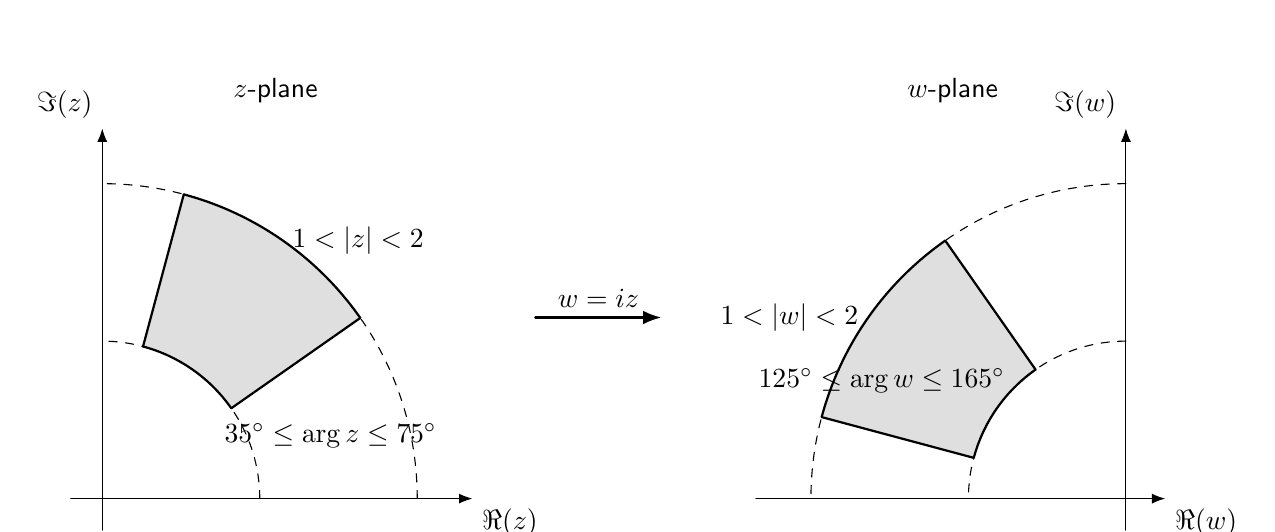
\begin{tikzpicture}[scale=2, >=Latex, line cap=round, line join=round]

% --- annular sector parameters in the z-plane ---
\def\rIn{1}
\def\rOut{2}
\def\aOne{35}   % degrees
\def\aTwo{75}   % degrees

% ------------------ LEFT: z-plane ------------------
\begin{scope}
  % axes
  \draw[->] (-0.2,0) -- (2.35,0) node[below right] {$\Re(z)$};
  \draw[->] (0,-0.2) -- (0,2.35) node[above left] {$\Im(z)$};

  % shaded annular sector:  aOne <= arg z <= aTwo, rIn <= |z| <= rOut
  % Build it as: outer arc from aOne to aTwo, then inner arc back from aTwo to aOne.
  \path[fill=gray!25, draw=none]
    ({\rOut*cos(\aOne)},{\rOut*sin(\aOne)}) arc (\aOne:\aTwo:\rOut)
    -- ({\rIn*cos(\aTwo)},{\rIn*sin(\aTwo)}) arc (\aTwo:\aOne:\rIn)
    -- cycle;

  % boundary curves of the annular sector
  \draw[thick]
    ({\rOut*cos(\aOne)},{\rOut*sin(\aOne)}) arc (\aOne:\aTwo:\rOut);
  \draw[thick]
    ({\rIn*cos(\aOne)},{\rIn*sin(\aOne)}) arc (\aOne:\aTwo:\rIn);

  % radial sides
  \draw[thick]
    ({\rIn*cos(\aOne)},{\rIn*sin(\aOne)}) -- ({\rOut*cos(\aOne)},{\rOut*sin(\aOne)});
  \draw[thick]
    ({\rIn*cos(\aTwo)},{\rIn*sin(\aTwo)}) -- ({\rOut*cos(\aTwo)},{\rOut*sin(\aTwo)});

  % optional dashed quarter arcs for reference
  \draw[dashed] (0,0) ++(0:\rIn) arc (0:90:\rIn);
  \draw[dashed] (0,0) ++(0:\rOut) arc (0:90:\rOut);

  % labels
  \node[above] at (1.1,2.45) {$z$-plane};
  \node[right] at ({\rOut*cos(55)},{\rOut*sin(55)}) {$1<|z|<2$};
  \node at (1.45,0.40) {$35^\circ \le \arg z \le 75^\circ$};
\end{scope}

% mapping arrow between the two diagrams
\draw[->, thick] (2.75,1.15) -- (3.55,1.15) node[midway,above] {$w=iz$};

% ------------------ RIGHT: w-plane ------------------
% Under w = i z, the region is rotated by +90 degrees:
% 35°..75°  --> 125°..165°  (in the second quadrant), radii unchanged.
\begin{scope}[xshift=6.5cm]
  % axes (space into negative real direction)
  \draw[->] (-2.35,0) -- (0.25,0) node[below right] {$\Re(w)$};
  \draw[->] (0,-0.2) -- (0,2.35) node[above left] {$\Im(w)$};

  % mapped angle range
  \pgfmathsetmacro{\bOne}{\aOne+90}
  \pgfmathsetmacro{\bTwo}{\aTwo+90}

  % shaded mapped annular sector
  \path[fill=gray!25, draw=none]
    ({\rOut*cos(\bOne)},{\rOut*sin(\bOne)}) arc (\bOne:\bTwo:\rOut)
    -- ({\rIn*cos(\bTwo)},{\rIn*sin(\bTwo)}) arc (\bTwo:\bOne:\rIn)
    -- cycle;

  % boundary curves
  \draw[thick]
    ({\rOut*cos(\bOne)},{\rOut*sin(\bOne)}) arc (\bOne:\bTwo:\rOut);
  \draw[thick]
    ({\rIn*cos(\bOne)},{\rIn*sin(\bOne)}) arc (\bOne:\bTwo:\rIn);

  % radial sides
  \draw[thick]
    ({\rIn*cos(\bOne)},{\rIn*sin(\bOne)}) -- ({\rOut*cos(\bOne)},{\rOut*sin(\bOne)});
  \draw[thick]
    ({\rIn*cos(\bTwo)},{\rIn*sin(\bTwo)}) -- ({\rOut*cos(\bTwo)},{\rOut*sin(\bTwo)});

  % optional dashed quadrant arcs for reference (now in quadrant II)
  \draw[dashed] (0,0) ++(90:\rIn) arc (90:180:\rIn);
  \draw[dashed] (0,0) ++(90:\rOut) arc (90:180:\rOut);

  % labels
  \node[above] at (-1.1,2.45) {$w$-plane};
  \node[left] at ({\rOut*cos(145)},{\rOut*sin(145)}) {$1<|w|<2$};
  \node at (-1.55,0.75) {$125^\circ \le \arg w \le 165^\circ$};
\end{scope}

\end{tikzpicture}

\end{example}

\newpage

\begin{example}
Show the effect of considering $w=z^2$ as a complex map that acts on the segment
$1\le |z| \le 2$, $35^\circ \le \arg z \le 75^\circ$ in the complex $z$ plane.

Again, polar form is useful. If $z = r e^{i \theta}$, then $w=r^2 e^{2 i \theta}$.

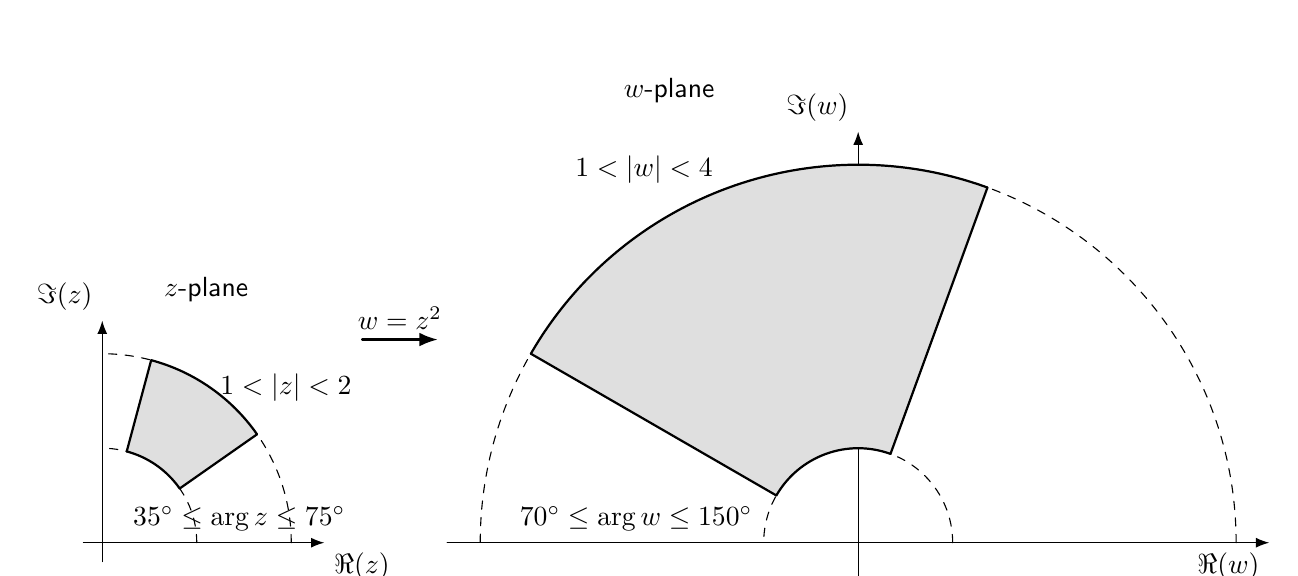
\begin{tikzpicture}[scale=1.2, >=Latex, line cap=round, line join=round]

% --- annular sector parameters in the z-plane ---
\def\rIn{1}
\def\rOut{2}
\def\aOne{35}   % degrees
\def\aTwo{75}   % degrees

% ------------------ LEFT: z-plane ------------------
\begin{scope}
  % axes
  \draw[->] (-0.2,0) -- (2.35,0) node[below right] {$\Re(z)$};
  \draw[->] (0,-0.2) -- (0,2.35) node[above left] {$\Im(z)$};

  % shaded annular sector in z-plane: aOne..aTwo, rIn..rOut
  \path[fill=gray!25, draw=none]
    ({\rOut*cos(\aOne)},{\rOut*sin(\aOne)}) arc (\aOne:\aTwo:\rOut)
    -- ({\rIn*cos(\aTwo)},{\rIn*sin(\aTwo)}) arc (\aTwo:\aOne:\rIn)
    -- cycle;

  % boundary curves
  \draw[thick]
    ({\rOut*cos(\aOne)},{\rOut*sin(\aOne)}) arc (\aOne:\aTwo:\rOut);
  \draw[thick]
    ({\rIn*cos(\aOne)},{\rIn*sin(\aOne)}) arc (\aOne:\aTwo:\rIn);

  % radial sides
  \draw[thick]
    ({\rIn*cos(\aOne)},{\rIn*sin(\aOne)}) -- ({\rOut*cos(\aOne)},{\rOut*sin(\aOne)});
  \draw[thick]
    ({\rIn*cos(\aTwo)},{\rIn*sin(\aTwo)}) -- ({\rOut*cos(\aTwo)},{\rOut*sin(\aTwo)});

  % dashed reference arcs for |z|=1,2 in first quadrant
  \draw[dashed] (0,0) ++(0:\rIn)  arc (0:90:\rIn);
  \draw[dashed] (0,0) ++(0:\rOut) arc (0:90:\rOut);

  % labels
  \node[above] at (1.1,2.45) {$z$-plane};
  \node at (1.45,0.25) {$35^\circ \le \arg z \le 75^\circ$};
  \node[right] at ({\rOut*cos(55)},{\rOut*sin(55)}) {$1<|z|<2$};
\end{scope}

% mapping arrow between the two diagrams
\draw[->, thick] (2.75,2.15) -- (3.55,2.15) node[midway,above] {$w=z^2$};

% ------------------ RIGHT: w-plane ------------------
% Under w = z^2:  |w| = |z|^2 so radii 1..2 map to 1..4,
% and arg(w) = 2 arg(z) so angles 35..75 map to 70..150 degrees.
\begin{scope}[xshift=8cm]
  % axes (need space into negative Re because the image reaches 150 degrees)
  \draw[->] (-4.35,0) -- (4.35,0) node[below left] {$\Re(w)$};
  \draw[->] (0,-0.35) -- (0,4.35) node[above left] {$\Im(w)$};

  \pgfmathsetmacro{\Rin}{\rIn*\rIn}
  \pgfmathsetmacro{\Rout}{\rOut*\rOut}
  \pgfmathsetmacro{\bOne}{2*\aOne}
  \pgfmathsetmacro{\bTwo}{2*\aTwo}

  % shaded image region in w-plane
  \path[fill=gray!25, draw=none]
    ({\Rout*cos(\bOne)},{\Rout*sin(\bOne)}) arc (\bOne:\bTwo:\Rout)
    -- ({\Rin*cos(\bTwo)},{\Rin*sin(\bTwo)}) arc (\bTwo:\bOne:\Rin)
    -- cycle;

  % boundary curves
  \draw[thick]
    ({\Rout*cos(\bOne)},{\Rout*sin(\bOne)}) arc (\bOne:\bTwo:\Rout);
  \draw[thick]
    ({\Rin*cos(\bOne)},{\Rin*sin(\bOne)}) arc (\bOne:\bTwo:\Rin);

  % radial sides
  \draw[thick]
    ({\Rin*cos(\bOne)},{\Rin*sin(\bOne)}) -- ({\Rout*cos(\bOne)},{\Rout*sin(\bOne)});
  \draw[thick]
    ({\Rin*cos(\bTwo)},{\Rin*sin(\bTwo)}) -- ({\Rout*cos(\bTwo)},{\Rout*sin(\bTwo)});

  % dashed reference arcs for |w|=1 and |w|=4 (upper half-plane)
  \draw[dashed] (0,0) ++(0:\Rin)  arc (0:180:\Rin);
  \draw[dashed] (0,0) ++(0:\Rout) arc (0:180:\Rout);

  % labels
  \node[above] at (-2.0,4.55) {$w$-plane};
  \node at (-2.35,0.25) {$70^\circ \le \arg w \le 150^\circ$};
  \node[left] at ({1.05*\Rout*cos(110)},{1.05*\Rout*sin(110)}) {$1<|w|<4$};
\end{scope}

\end{tikzpicture}
\end{example}






\begin{example}
We can use a complex function to convert a circle (with certain properties) to an aerofoil shape. Each dot on the left plot (the $z$ values) is connected to one on the right (the $w$ values) by the formula
\begin{equation*}
\label{eqn:comptrans}
w(z) = \frac{1}{2}\left(z + \frac{1}{z}\right).
\end{equation*}
The highlighted circles and diamonds show where their $z$ values end up on the $w$ value plot.
Note that the circle in the $z$ plane is slightly off-centre.

\begin{minipage}{0.5\textwidth}
\begin{center}
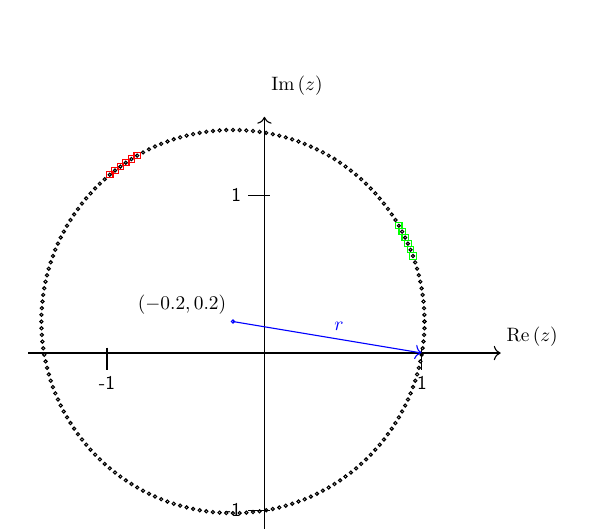
\begin{tikzpicture}[scale=2, declare function={xx(\a,\b) = 1/2*\a*(\a*\a + \b*\b + 1)/(\a*\a + \b*\b); yy(\a,\b) = 1/2*\b*(\a*\a + \b*\b - 1)/(\a*\a + \b*\b);},]
	  \draw[->] (-1.5,0) -- (1.5,0) ; \node[above,scale=0.7] at (1.7,0) {$\RE{z}$};
    \draw[->] (0,-1.2) -- (0,1.5) ; \node[right,scale=0.7] at (0,1.7) {$\IM{z}$}; 
		\foreach \x in {-1,1}
					\draw (\x,1pt) -- (\x,-3pt) node[anchor=north,scale=0.7] {\x};
    \foreach \y in {-1,1}
					\draw (1pt,\y) -- (-3pt,\y) node[anchor=east,scale=0.7] {\y};
	
\def\xshift{0.2} %>0
\def\yshift{0.2} %>0
\def\radius{sqrt((1+\xshift)*(1+\xshift) + (\yshift*\yshift))}
\draw[\blue,->]  (-\xshift,\yshift) -- (1,0) node[midway, above right,scale=0.7] {$r$};
\draw[\blue] (-\xshift,\yshift) circle (0.01); \node[above left,scale=0.7] at  (-\xshift,\yshift) {$(-\xshift, \yshift)$};

\foreach \ii in {0,2,4,...,360} {
\def\real{\radius*cos(\ii)-\xshift}
\def\imag{\radius*sin(\ii)+\yshift}
\draw ({\real},{\imag}) circle (0.01);
}

\foreach \ii in {20,22,...,30} {
\def\real{\radius*cos(\ii)-\xshift}
\def\imag{\radius*sin(\ii)+\yshift}
\draw[\green] ({\real-0.02},{\imag-0.02}) rectangle ++(0.04,0.04);
}

\foreach \ii in {120,122,...,130} {
\def\real{\radius*cos(\ii)-\xshift}
\def\imag{\radius*sin(\ii)+\yshift}
\draw[\red] ({\real-0.02},{\imag-0.02}) rectangle ++(0.04,0.04);
}
\end{tikzpicture}
\end{center}
\end{minipage}%
\begin{minipage}{0.5\textwidth}
\begin{center}
\begin{tikzpicture}[scale=2, declare function={xx(\a,\b) = 1/2*\a*(\a*\a + \b*\b + 1)/(\a*\a + \b*\b); yy(\a,\b) = 1/2*\b*(\a*\a + \b*\b - 1)/(\a*\a + \b*\b);},]
	  \draw[->] (-1.5,0) -- (1.5,0) ; \node[above,scale=0.7] at (1.7,0) {$\RE{w}$};
    \draw[->] (0,-1.2) -- (0,1.5) ; \node[right,scale=0.7] at (0,1.7) {$\IM{w}$}; 
		\foreach \x in {-1,1}
					\draw (\x,1pt) -- (\x,-3pt) node[anchor=north,scale=0.7] {\x};
    \foreach \y in {-1,1}
					\draw (1pt,\y) -- (-3pt,\y) node[anchor=east,scale=0.7] {\y};
	
\def\xshift{0.2} %>0
\def\yshift{0.2} %>0
\def\radius{sqrt((1+\xshift)*(1+\xshift) + (\yshift*\yshift))}
%\draw[\blue,->]  (-\xshift,\yshift) -- (1,0) node[midway, above right,scale=0.7] {$r$};
%\draw[\blue] (-\xshift,\yshift) circle (0.01); \node[above left,scale=0.7] at  (-\xshift,\yshift) {$(-\xshift, \yshift)$};

\foreach \ii in {0,2,4,...,360} {
\def\real{\radius*cos(\ii)-\xshift}
\def\imag{\radius*sin(\ii)+\yshift}
\draw ({xx(\real,\imag)},{yy(\real,\imag)}) circle (0.01);
%\draw ({\real},{\imag}) circle (0.01);
}

\foreach \ii in {20,22,...,30} {
\def\real{\radius*cos(\ii)-\xshift}
\def\imag{\radius*sin(\ii)+\yshift}
\draw[\green] ({xx(\real,\imag)-0.02},{yy(\real,\imag)-0.02}) rectangle ++(0.04,0.04);
%\draw[\green] ({\real-0.02},{\imag-0.02}) rectangle ++(0.04,0.04);
}

\foreach \ii in {120,122,...,130} {
\def\real{\radius*cos(\ii)-\xshift}
\def\imag{\radius*sin(\ii)+\yshift}
\draw[\red] ({xx(\real,\imag)-0.02},{yy(\real,\imag)-0.02}) rectangle ++(0.04,0.04);
%\draw[\red] ({\real-0.02},{\imag-0.02}) rectangle ++(0.04,0.04);
}
\end{tikzpicture}
\end{center}

\end{minipage}%


\(w(z)\) in this example is a {\it complex} function. The argument \(z\) is a complex number and the function returns a complex number \(w(z)\). 




Let us pick apart \( w(z)\) in Cartesian form. 
\begin{align*}
w(z) &= \frac{1}{2}\left(z + \frac{1}{z}\right) = \frac{1}{2}\left(x + i y + \frac{1}{x+iy}\right)\\
     &= \frac{1}{2}\left(x + i y + \frac{x-iy}{x^2+y^2}\right)\\
     &= \frac{1}{2}\left(x + \frac{x}{x^2+y^2} + i \left( y - \frac{y}{x^2+y^2} \right) \right)
\end{align*}

We can see that the {\it complex} function \( w(z)\) may be written using two {\it real}-valued functions of \(x,y\)
\[
w(z) = u(x,y) + i v(x,y)  
\]
where
\[
u(x,y) = x + \frac{x}{x^2+y^2}, \qquad v(x,y) =  y - \frac{y}{x^2+y^2}
\]
This is true in general.
\end{example}

\begin{example}
Let the initial circle now be centred on the origin with radius $R$, i.e. \(|z|=R\) with \(R>0\).  
What is \(w(z)\)?

Parametrize it by
\[
z = R e^{i\theta}, \qquad 0\le \theta < 2\pi .
\]
Then
\begin{align*}
w(z)
&= \frac12\left(z+\frac1z\right)
 = \frac12\left(R e^{i\theta} + \frac{1}{R}e^{-i\theta}\right) \\
&= \frac12\Big((R+\tfrac1R)\cos\theta \;+\; i\,(R-\tfrac1R)\sin\theta\Big).
\end{align*}
Writing \(w=u+iv\), we have
\[
u=\frac{R+\frac1R}{2}\cos\theta,
\qquad
v=\frac{R-\frac1R}{2}\sin\theta.
\]
Eliminating \(\theta\) gives
\[
\frac{u^2}{\left(\frac{R+\frac1R}{2}\right)^2}
+
\frac{v^2}{\left(\frac{|R-\frac1R|}{2}\right)^2}
=1.
\]
Hence the image of the circle \(|z|=R\) under \(w(z)=\tfrac12(z+1/z)\) is an ellipse
centered at the origin, with semiaxes
\[
a=\frac{R+\frac1R}{2} \quad\text{(along the real axis)},\qquad
b=\frac{|R-\frac1R|}{2} \quad\text{(along the imaginary axis)}.
\]
In the special case \(R=1\), the ellipse degenerates to the line segment.
\[
w=\cos\theta\in[-1,1].
\]


% Requires: \usepackage{tikz}
% (and your colour macros \blue,\red,\green or replace them by e.g. blue,red,green)

\begin{minipage}{0.5\textwidth}
\begin{center}
\begin{tikzpicture}[scale=2]
  % axes in the z-plane
  \draw[->] (-1.6,0) -- (1.6,0) ; \node[above,scale=0.7] at (1.8,0) {$\RE{z}$};
  \draw[->] (0,-1.4) -- (0,1.6) ; \node[right,scale=0.7] at (0,1.8) {$\IM{z}$};

  \foreach \x in {-1,1}
    \draw (\x,1pt) -- (\x,-3pt) node[anchor=north,scale=0.7] {\x};
  \foreach \y in {-1,1}
    \draw (1pt,\y) -- (-3pt,\y) node[anchor=east,scale=0.7] {\y};

  % circle |z|=R
  \def\R{1.25}
  \draw[\blue,thick] (0,0) circle (\R);
  \node[above right,scale=0.7] at ({\R/sqrt(2)},{\R/sqrt(2)}) {$|z|=R$};

  % a couple of highlighted arcs on the circle (like your style)
  \foreach \ii in {20,22,...,30} {
    \def\real{\R*cos(\ii)}
    \def\imag{\R*sin(\ii)}
    \draw[\green] ({\real-0.02},{\imag-0.02}) rectangle ++(0.04,0.04);
  }
  \foreach \ii in {120,122,...,130} {
    \def\real{\R*cos(\ii)}
    \def\imag{\R*sin(\ii)}
    \draw[\red] ({\real-0.02},{\imag-0.02}) rectangle ++(0.04,0.04);
  }
\end{tikzpicture}
\end{center}
\end{minipage}%
\begin{minipage}{0.5\textwidth}
\begin{center}
\begin{tikzpicture}[scale=2]
  % axes in the w-plane
  \draw[->] (-1.6,0) -- (1.6,0) ; \node[above,scale=0.7] at (1.8,0) {$\RE{w}$};
  \draw[->] (0,-1.4) -- (0,1.6) ; \node[right,scale=0.7] at (0,1.8) {$\IM{w}$};

  \foreach \x in {-1,1}
    \draw (\x,1pt) -- (\x,-3pt) node[anchor=north,scale=0.7] {\x};
  \foreach \y in {-1,1}
    \draw (1pt,\y) -- (-3pt,\y) node[anchor=east,scale=0.7] {\y};

  % parameters: image ellipse semi-axes
  \def\R{1.25}
  \pgfmathsetmacro{\a}{0.5*(\R + 1/\R)}   % semi-axis on Re(w)
  \pgfmathsetmacro{\b}{0.5*abs(\R - 1/\R)}% semi-axis on Im(w)

  % draw the image ellipse
  \draw[\blue,thick] (0,0) ellipse ({\a} and {\b});
  \node[above right,scale=0.7] at ({\a/sqrt(2)},{\b/sqrt(2)}) {$w=\tfrac12(z+1/z)$};

  % optional: show the focal points (always at \pm 1)
  %\draw (1,0) circle (0.01); \draw (-1,0) circle (0.01);
  %\node[below,scale=0.7] at (1,0) {$1$};
  %\node[below,scale=0.7] at (-1,0) {$-1$};

  % matching highlighted arcs on the ellipse (same theta ranges)
  \foreach \ii in {20,22,...,30} {
    \def\real{\a*cos(\ii)}
    \def\imag{\b*sin(\ii)}
    \draw[\green] ({\real-0.02},{\imag-0.02}) rectangle ++(0.04,0.04);
  }
  \foreach \ii in {120,122,...,130} {
    \def\real{\a*cos(\ii)}
    \def\imag{\b*sin(\ii)}
    \draw[\red] ({\real-0.02},{\imag-0.02}) rectangle ++(0.04,0.04);
  }
\end{tikzpicture}
\end{center}
\end{minipage}%
    
\end{example}

\begin{exercise}{}
    Consider the {\it quadratic map}, $f(z) = z^2 +c$ where $c=a+ib$ (with $a,b$ real) is a complex constant. 
    
    What is $f(z)$ when written in terms of real functions $g,h$. i.e. $f(z)= f(x+iy) = g(x,y) + i h(x,y)$? 
\end{exercise}

\begin{solution}
    Substitute $z=x+iy$ into $f(z)=z^2 + c$ and gather the real and imaginary parts:
    \begin{eqnarray*}
        f(z) &= f(z+iy) = (x+iy)^2 + a + ib \\
        &= (x^2 - y^2 + a) + i (2  xy +b) 
    \end{eqnarray*}
   hence $g(x,y) = x^2 - y^2 + a$ and $h(x,y) = 2  xy +b $
\end{solution}

%------------------------------------------------------------
\subsection{Iterating complex maps}

One of the most striking uses of complex numbers is in \emph{complex dynamics}, where we repeatedly apply a map
\[
z_{n+1}=f(z_n),\qquad n=0,1,2,\dots
\]
starting from some initial value \(z_0\in\mathbf{C}\).  The resulting sequence \(\{z_n\}\) is called the \emph{orbit} of \(z_0\).
Even very simple choices of \(f\) can produce complicated behaviour: orbits may converge to a fixed point, fall into a
periodic cycle, or escape to infinity.

\medskip
We have just encountered the \emph{quadratic map}
\[
f_c(z)=z^2+c,
\]
where \(c\in\mathbf{C}\) is a complex parameter.  A useful practical fact is the \emph{escape radius}:
if at some step \(|z_n|>2\) (when \( | c | < 2 \)), then the orbit will diverge to infinity (so we do not need to keep iterating).

\begin{example}
If we consider a few iterates in the complex plane: Take \(c=-0.123+0.745\,i\) and start at \(z_0=0\). The first few iterates are
\[
z_1=c,\qquad
z_2\approx -0.6629+0.5617\,i,\qquad
z_3\approx 8.9\times10^{-4}+2.6\times10^{-4}\,i,
\]
and then the orbit returns close to \(z_1\) and \(z_2\) again.
\end{example}


\begin{example}
Julia sets (bounded starting points):
Fix \(c\in\mathbf{C}\).  The \emph{filled Julia set} \(K_c\) is the set of starting values 
\(z_0\) whose orbits under
\(z_{n+1}=z_n^2+c\) stay bounded.  (The \emph{Julia set} \(J_c\) is the boundary of \(K_c\).)
The picture below is a coarse ``escape-time'' plot for \(c=-1\): points \(z_0\) that do \emph{not} escape after a fixed
number of iterations (200) are drawn as yellow dots.

\begin{center}
\includegraphics[width=0.5\textwidth]{julia_c_minus1.png}
\end{center}
\end{example}

\begin{example}

The Mandelbrot set (bounded parameters):

Instead of fixing \(c\) and varying \(z_0\), we can fix the starting point \(z_0=0\) and vary the parameter \(c\).
The \emph{Mandelbrot set} \(M\) is the set of parameters \(c\) for which the orbit of \(0\) under \(z_{n+1}=z_n^2+c\)
remains bounded.  The plot below is again an escape-time picture (very low resolution), now in the \(c\)-plane.

\begin{center}
\includegraphics[width=0.5\textwidth]{mandelbrot.png}
\end{center}
\end{example}
\section{An aside: Quaternions}

Complex numbers extend the real numbers by adjoining a new unit $i$ with $i^2=-1$.  Quaternions extend the complex numbers further by adjoining \emph{three} imaginary units.

Quaternions were introduced by the Irish mathematician William Rowan Hamilton in 1843 as a way to extend complex numbers to describe rotations in three dimensions. After years of trying (and failing) to build a consistent “three–dimensional complex arithmetic”, Hamilton realised that the key was to move to four components and to accept that multiplication need not commute. On 16th October 1843, while walking in Dublin, he famously carved the fundamental relations 
\begin{equation*}
\mathbf{i}^2=\mathbf{j}^2=\mathbf{k}^2=\mathbf{i}\mathbf{j}\mathbf{k}=-1.
\end{equation*}
into the stone of Brougham Bridge. 
\begin{center}
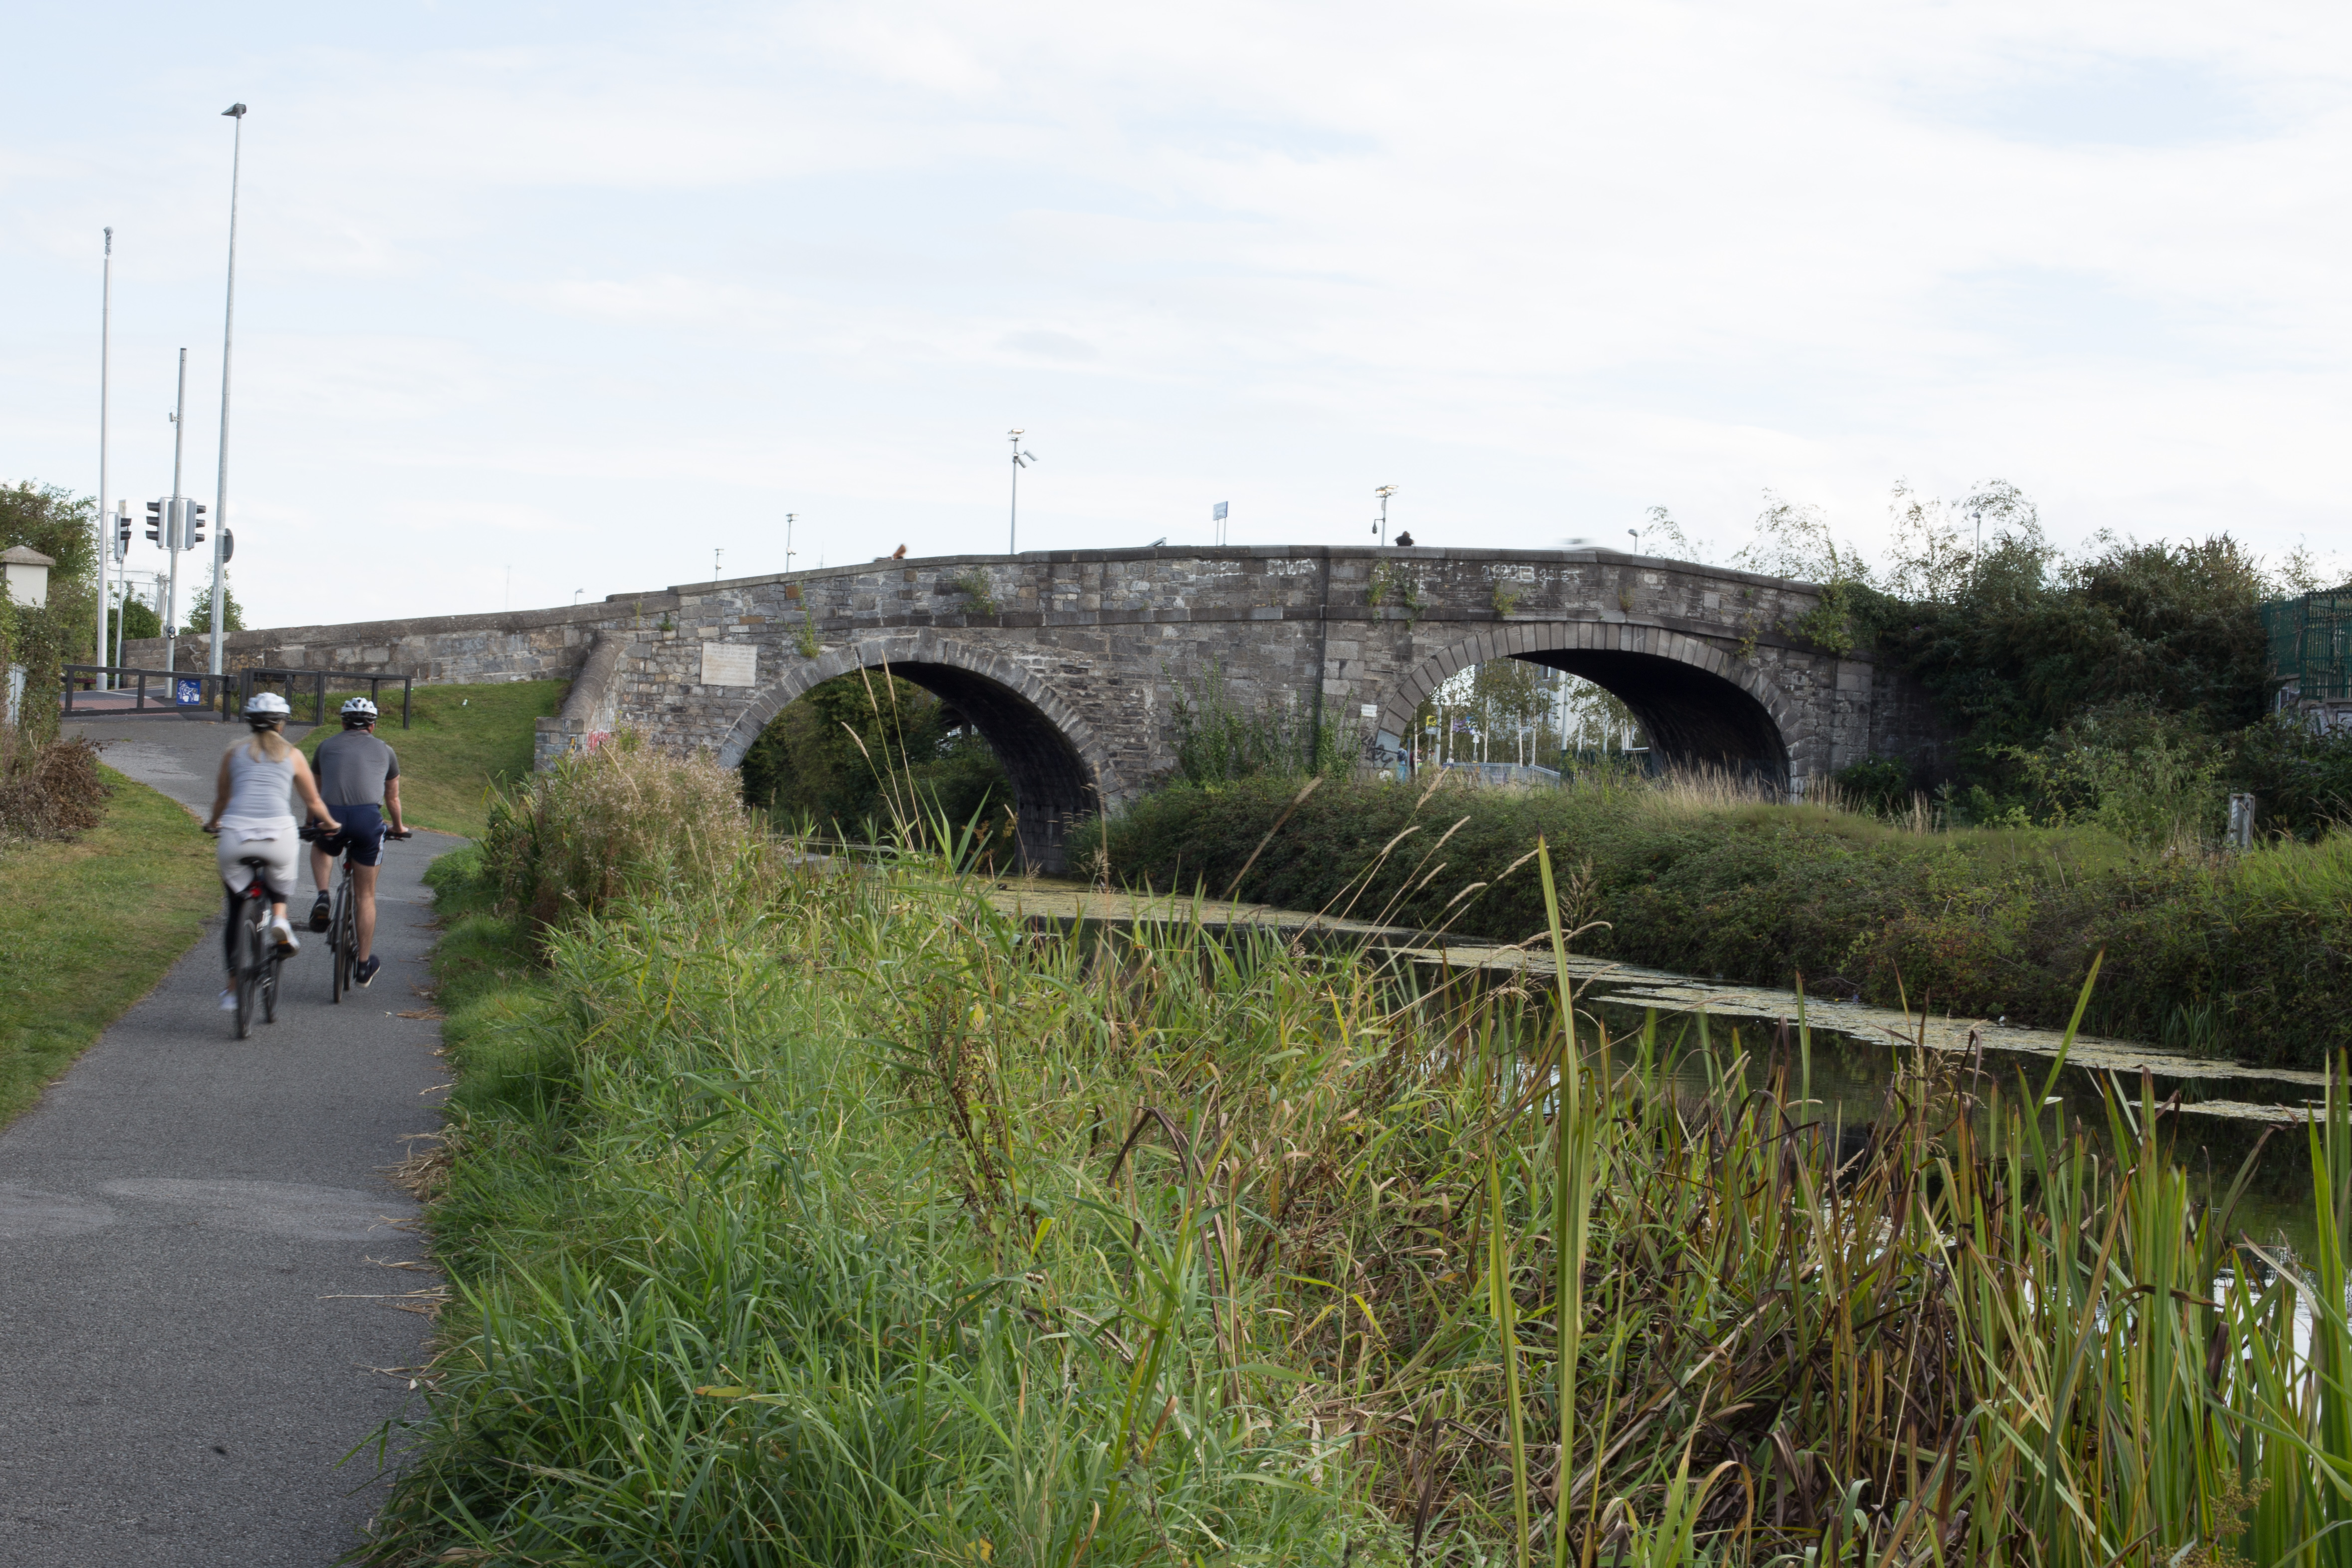
\includegraphics[width=0.5\textwidth]{Broom_Bridge.jpg}
\end{center}

Quaternions quickly attracted attention in 19th-century mathematical physics and geometry, but they were later overshadowed in many applications by the vector calculus of Gibbs and Heaviside. In the late 20th century they saw a major revival in engineering and computing—especially in robotics, aerospace, and computer graphics—because unit quaternions provide a numerically stable and efficient way to represent 3D rotations without the singularities that can occur with Euler angles, which appear when using vectors.

\subsection{Definitions and Arithmetic}

\begin{df}{Quaternion}
A \emph{quaternion} is an expression of the form
\begin{equation*}
q = a + b\,\mathbf{i} + c\,\mathbf{j} + d\,\mathbf{k}
\end{equation*}
where $a,b,c,d\in\R$ and the symbols $\mathbf{i},\mathbf{j},\mathbf{k}$ satisfy
\begin{equation*}
\mathbf{i}^2=\mathbf{j}^2=\mathbf{k}^2=\mathbf{i}\mathbf{j}\mathbf{k}=-1.
\end{equation*}
The set of all quaternions is denoted $\mathbb H$.
\end{df}

From the defining relations one can derive the multiplication rules
\begin{center}
\renewcommand{\arraystretch}{1.2}
\begin{tabular}{c|ccc}
$\cdot$ & $\mathbf{i}$ & $\mathbf{j}$ & $\mathbf{k}$\\
\hline
$\mathbf{i}$ & $-1$ & $\mathbf{k}$ & $-\mathbf{j}$\\
$\mathbf{j}$ & $-\mathbf{k}$ & $-1$ & $\mathbf{i}$\\
$\mathbf{k}$ & $\mathbf{j}$ & $-\mathbf{i}$ & $-1$\\
\end{tabular}
\end{center}

\caution Quaternion multiplication is \emph{not commutative}. For example,
\begin{equation*}
\mathbf{i}\mathbf{j}=\mathbf{k}\qquad\text{but}\qquad \mathbf{j}\mathbf{i}=-\mathbf{k}.
\end{equation*}

\begin{df}{Scalar and vector parts}
Write a quaternion as
\begin{equation*}
q = a + \vec v,\qquad \text{where}\quad \vec v=b\,\mathbf{i}+c\,\mathbf{j}+d\,\mathbf{k}.
\end{equation*}
We call $a$ the \emph{scalar part} of $q$ and $\vec v$ the \emph{vector part}.
\end{df}

Addition and subtraction are componentwise (exactly as for complex numbers):
\begin{equation*}
(a,\,b,\,c,\,d)\pm (e,\,f,\,g,\,h)=(a\pm e,\,b\pm f,\,c\pm g,\,d\pm h).
\end{equation*}
Multiplication is defined using distributivity together with the table above.

\begin{example}
Compute $(1+\mathbf{i})(1+\mathbf{j})$.
\begin{align*}
(1+\mathbf{i})(1+\mathbf{j})&=1+\mathbf{j}+\mathbf{i}+\mathbf{i}\mathbf{j}\\
&=1+\mathbf{i}+\mathbf{j}+\mathbf{k}.
\end{align*}
If we swap the factors,
\begin{align*}
(1+\mathbf{j})(1+\mathbf{i})&=1+\mathbf{i}+\mathbf{j}+\mathbf{j}\mathbf{i}\\
&=1+\mathbf{i}+\mathbf{j}-\mathbf{k},
\end{align*}
so the order matters.
\end{example}

\subsection{Conjugate, Norm and Inverse}

Quaternions have an analogue of complex conjugation.

\begin{df}{Quaternion conjugate}
For $q=a+b\mathbf{i}+c\mathbf{j}+d\mathbf{k}$, the \emph{conjugate} is
\begin{equation*}
\conj{q}=a-b\mathbf{i}-c\mathbf{j}-d\mathbf{k}.
\end{equation*}
\end{df}

\begin{df}{Norm}
The \emph{norm} of $q$ is defined by
\begin{equation*}
\lVert q\rVert = \sqrt{q\conj{q}}=\sqrt{a^2+b^2+c^2+d^2}.
\end{equation*}
\end{df}

\begin{example}
Let $q=2-\mathbf{i}+2\mathbf{j}+\mathbf{k}$. Then
\begin{align*}
\conj{q}&=2+\mathbf{i}-2\mathbf{j}-\mathbf{k},\\
\lVert q\rVert&=\sqrt{2^2+(-1)^2+2^2+1^2}=\sqrt{10}.
\end{align*}
\end{example}

Just like complex numbers, the norm is useful for division.

\begin{thm}{Inverse of a nonzero quaternion}
If $q\neq 0$, then $q$ has a multiplicative inverse
\begin{equation*}
q^{-1}=\frac{\conj{q}}{\lVert q\rVert^2}.
\end{equation*}
\end{thm}

\begin{example}
Find the inverse of $q=1+\mathbf{i}+\mathbf{j}+\mathbf{k}$.
\begin{align*}
\conj{q}&=1-\mathbf{i}-\mathbf{j}-\mathbf{k},\\
\lVert q\rVert^2&=1^2+1^2+1^2+1^2=4,\\
q^{-1}&=\frac{1}{4}\,(1-\mathbf{i}-\mathbf{j}-\mathbf{k}).
\end{align*}
\end{example}

\caution Because multiplication is not commutative, one must distinguish between left and right division in more advanced settings. In this course we will only divide by placing the inverse on the \emph{right}: $\,p/q:=p\,q^{-1}$.

\subsection{Unit Quaternions and 3D Rotations}

A key application of quaternions is the description of rotations in $\R^3$.

\begin{df}{Pure imaginary quaternion}
A quaternion with zero scalar part,
\begin{equation*}
\vec v=b\mathbf{i}+c\mathbf{j}+d\mathbf{k},
\end{equation*}
is called \emph{pure imaginary}.  We identify it with the vector $(b,c,d)\in\R^3$.
\end{df}

\begin{df}{Unit quaternion}
A quaternion $q$ with $\lVert q\rVert=1$ is called a \emph{unit quaternion}.
\end{df}

Any rotation by angle $\theta$ about a unit axis $\hat n\in\R^3$ can be encoded by the unit quaternion
\begin{equation*}
q = \cos\frac{\theta}{2} + \sin\frac{\theta}{2}\,(n_1\mathbf{i}+n_2\mathbf{j}+n_3\mathbf{k}),\qquad \hat n=(n_1,n_2,n_3),\ \lVert\hat n\rVert=1.
\end{equation*}
Given a vector $\vec v\in\R^3$ (viewed as a pure imaginary quaternion), the rotated vector is
\begin{equation*}
\vec v\,' = q\,\vec v\,q^{-1}.
\end{equation*}

\begin{example}
Rotate $(1,0,0)$ by $90^\circ$ about the $z$--axis.

The axis is $\hat n=(0,0,1)$ and $\theta=\pi/2$, so
\begin{equation*}
q=\cos\frac{\pi}{4}+\sin\frac{\pi}{4}\,\mathbf{k}=\frac{\sqrt 2}{2}+\frac{\sqrt 2}{2}\,\mathbf{k},\qquad q^{-1}=\conj{q}=\frac{\sqrt 2}{2}-\frac{\sqrt 2}{2}\,\mathbf{k}.
\end{equation*}
Let $\vec v=\mathbf{i}$ (since $(1,0,0)$ corresponds to $\mathbf{i}$). Then
\begin{align*}
\vec v\,' &= q\,\mathbf{i}\,q^{-1}
=\left(\tfrac{\sqrt2}{2}+\tfrac{\sqrt2}{2}\mathbf{k}\right)\mathbf{i}\left(\tfrac{\sqrt2}{2}-\tfrac{\sqrt2}{2}\mathbf{k}\right)\\
&=\left(\tfrac{\sqrt2}{2}\mathbf{i}+\tfrac{\sqrt2}{2}\mathbf{k}\mathbf{i}\right)\left(\tfrac{\sqrt2}{2}-\tfrac{\sqrt2}{2}\mathbf{k}\right)
=\left(\tfrac{\sqrt2}{2}\mathbf{i}+\tfrac{\sqrt2}{2}\mathbf{j}\right)\left(\tfrac{\sqrt2}{2}-\tfrac{\sqrt2}{2}\mathbf{k}\right)\\
&= \mathbf{j}.
\end{align*}
Thus $(1,0,0)$ rotates to $(0,1,0)$, as expected.
\end{example}

\secbreak

\begin{exercise}{}
Use the multiplication table to compute $\mathbf{i}\mathbf{k}$ and $\mathbf{k}\mathbf{i}$. What do you notice?
\end{exercise}
\begin{solution}
From the table, $\mathbf{i}\mathbf{k}=-\mathbf{j}$ and $\mathbf{k}\mathbf{i}=\mathbf{j}$. They differ by a minus sign, illustrating non-commutativity.
\end{solution}

\begin{exercise}{}
Let $q=3-2\mathbf{i}+\mathbf{j}$. Compute $\conj{q}$, $\lVert q\rVert$, and $q^{-1}$.
\end{exercise}
\begin{solution}
We have $\conj{q}=3+2\mathbf{i}-\mathbf{j}$ and
\begin{equation*}
\lVert q\rVert=\sqrt{3^2+(-2)^2+1^2+0^2}=\sqrt{14}.
\end{equation*}
Hence
\begin{equation*}
q^{-1}=\frac{\conj{q}}{\lVert q\rVert^2}=\frac{1}{14}\,(3+2\mathbf{i}-\mathbf{j}).
\end{equation*}
\end{solution}

\begin{exercise}{}
Let $\hat n=(1,0,0)$ and $\theta=\pi$. Write down the unit quaternion $q$ describing rotation by $\pi$ about the $x$--axis, and compute $q\,\mathbf{j}\,q^{-1}$.
\end{exercise}
\begin{solution}
Here $q=\cos(\pi/2)+\sin(\pi/2)\,\mathbf{i}=\mathbf{i}$ and $q^{-1}=\conj{q}=-\mathbf{i}$.
Then
\begin{equation*}
q\,\mathbf{j}\,q^{-1}=\mathbf{i}\,\mathbf{j}\,(-\mathbf{i})=-(\mathbf{i}\mathbf{j})\mathbf{i}=-\mathbf{k}\mathbf{i}=-\mathbf{j}.
\end{equation*}
So the $y$--axis is sent to $-y$, as expected for a $180^\circ$ rotation about the $x$--axis.
\end{solution}

\section{Vectors, Spans and Bases in $\FR^2$, $\FR^3$ and $\FR^n$.}

    \subsection{Vectors in $\FR^2$}
	We briefly recall some facts about vectors in $\FR^2$. Intuitively, a \textit{vector} of $\FR^2$ can be thought as an arrow encoding a length and a direction. A vector however does not have an origin, so one may draw many arrows in the plane corresponding to the same vector:
	
	\begin{equation*}
	\begin{picture}(70,70)
	\put(0.0,8.0){\line(1,0){70}}
	\put(8.0,0.0){\line(0,1){70}}
	\put(8.0,8.0){\vector(2,1){50}}
	\put(58.0,15.0){\vector(2,1){50}}
	\put(22.0,40.0){\vector(2,1){50}}
	%\put(2.0,0.0){\makebox(0,0)[c]{$\nv$}}
	\put(33.0,10.0){\line(0,-1){4}}
	\put(58.0,10.0){\line(0,-1){4}}
	\put(6.0,33.0){\line(1,0){4}}
	\put(6.0,58.0){\line(1,0){4}}
	%\put(0.0,33.0){\makebox(0,0)[c]{$v_2$}}
	%\put(58.0,0.0){\makebox(0,0)[c]{$v_1$}}
	\end{picture}
	\end{equation*}
	
	One may identify the set of all vectors in $\FR^2$ with the set of points of the plane $\FR^2$, by associating to each point of the plane the vector from the origin to that point. Under this identification, the origin corresponds to a vector called the \textit{null vector} and denoted $\nv$. 

    \begin{df}{}
	Each point and thus each vector $\vv\in\FR^2$ can be denoted by a pair of real numbers (thus the notation $\FR^2$): the horizontal displacement and the vertical displacement. Such a vector is denoted  by the $2 \times 1$ matrix
	\begin{equation*}
	\vv=\vectt{v_1}{v_2}~.
	\end{equation*}
	
	
	\begin{equation*}
	\begin{picture}(70,70)
	\put(0.0,8.0){\line(1,0){70}}
	\put(8.0,0.0){\line(0,1){70}}
	\put(8.0,8.0){\vector(2,1){50}}
	%\put(2.0,0.0){\makebox(0,0)[c]{$\nv$}}
	\put(33.0,10.0){\line(0,-1){4}}
	\put(58.0,10.0){\line(0,-1){4}}
	\put(6.0,33.0){\line(1,0){4}}
	\put(6.0,58.0){\line(1,0){4}}
	\put(0.0,33.0){\makebox(0,0)[c]{$v_2$}}
	\put(58.0,0.0){\makebox(0,0)[c]{$v_1$}}
	\end{picture}
	\end{equation*}
	
	
	It is a very useful convention to write vectors vertically, i.e. as $2 \times 1$ matrices. For typesetting reasons however, we often write that vector as $\vv=(v_1,v_2)^T$, i.e. as a $1\times 2$ matrix instead. 
	\end{df}
	
	We have the following rules for adding two vectors $\vv=(v_1,v_2)^T$ and $\wv=(w_1,w_2)^T$ and for multiplying a vector by a number $\lambda\in \FR$ (called a \textit{scalar}):
	\begin{equation*}
	\vv+\wv=\vectt{v_1}{v_2}+\vectt{w_1}{w_2}:=\vectt{v_1+w_1}{v_2+w_2}\eand \lambda \vv:=\vectt{\lambda v_1}{\lambda v_2}~.
	\end{equation*}
	\begin{equation*}
	\begin{picture}(200,150)(0,50)
	\put(0.0,100.0){\line(1,0){200}}
	\put(100.0,50.0){\line(0,1){150}}
	\put(100.0,100.0){\vector(1,3){30}}
	\put(100.0,100.0){\vector(3,-1){45}}
	\put(100.0,100.0){\vector(-3,1){90}}
	\put(130.0,190.0){\vector(3,-1){45}}
	\put(100.0,100.0){\vector(1,1){75}}
	\put(95.0,92.0){\makebox(0,0)[c]{$\nv$}}
	\put(120.0,180.0){\makebox(0,0)[c]{$\vv_1$}}
	\put(185.0,160.0){\makebox(0,0)[c]{$\vv_1+\vv_2$}}
	\put(140.0,80.0){\makebox(0,0)[c]{$\vv_2$}}
	\put(30.0,130.0){\makebox(0,0)[c]{$-2\vv_2$}}
	\end{picture}
	\end{equation*}
	
	With our convention, the null vector is the vector with coordinates $(0,0)^T$. Note that if we multiply a vector by  $0$, we obtain the null vector: $0\vv=\nv$ for all $\vv\in\FR^2$.
	
%	\paragraph{Scalar product and norm.} We mentioned that a vector in $\FR^2$ encodes a notion of length. We now make this precise. We introduce the  \textit{scalar product} (or  \textit{Euclidean inner product}) $\langle\cdot,\cdot\rangle:\FR^2\times \FR^2\rightarrow\FR$ defined as
%	\begin{equation*}
%	\langle\vectt{u_1}{u_2}, \vectt{v_1}{v_2}\rangle:=u_1v_1+u_2v_2~.
%	\end{equation*}
%	If we take the inner product of a vector $\vv$ with itself, $\langle \vv,\vv \rangle$, we obtain the square of the length\footnote{To see this, draw a picture, insert the coordinates of the vector $\vv$ and use Pythagoras' theorem.} of this vector. We call the length of a vector its \textit{norm} and define
%	\begin{equation*}
%	||\vv||:=\sqrt{\langle \vv,\vv\rangle}~.
%	\end{equation*}
	
	
	
%	\paragraph{Angles.} For parallel vectors $\vv,\wv\in\FR^2$, we have the formula $\langle \vv,\wv\rangle=||\vv||\cdot||\wv||$. More generally we have: 
%%	 and the above lemma states that for perpendicular vectors $\vv,\wv$, it is $\langle \vv,\wv\rangle=0$. These are extreme cases of the general formula
%\begin{prop} For vectors $\uv, \vv $ of $\FR^2$, we have
%	\begin{equation*}
%	\langle \vv,\wv\rangle=||\vv||\cdot||\wv||\cos(\vv,\wv)~,
%	\end{equation*}
%	where $\cos(\vv,\wv)$ denotes the cosine of the angle between $\vv$ and $\wv$.
%	\end{prop}
%%	where $\cos(\vv,\wv)$ denotes the cosine of the angle between $\vv$ and $\wv$. 
%\begin{proof} Uusing coordinates, one gets 
%	\begin{equation*}\label{eq:PythagorasR2}
%	||\vv - \wv||^2 = v_1^2+v_2^2-2v_1w_1-2v_2w_2+w_1^2+w_2^2=||\vv||^2 + ||\wv||^2 -2\langle \vv,\wv\rangle~.
%	\end{equation*}
%	We also know from the law of cosines that, given the triangle spanned by $\vv$ and $\wv$, with sides $||\vv||$, $||\wv||$, $||\vv - \wv||$ and angle $\theta$ opposing side $||\vv - \wv||$, we have
%	\begin{equation*}
%	||\vv - \wv||^2=||\vv||^2 + ||\wv||^2-2||\vv||.||\wv||\cos(\theta)~
%	\end{equation*}
%and the result follows.
%	\end{proof}
%	
%	\begin{prop} Two vectors are perpendicular if and only if their inner product vanishes.\end{prop}
%	\begin{proof}
%		By Pythagoras' theorem, two vectors $\vv,\wv\in\FR^2$ are perpendicular if and only if we have $||\vv||^2+||\wv||^2=||\vv+\wv||^2$. In coordinates, this is equivalent to
%		\begin{equation*}\label{eq:PythagorasR2}
%		v_1^2+v_2^2+w_1^2+w_2^2=v_1^2+v_2^2+2v_1w_1+2v_2w_2+w_1^2+w_2^2=v_1^2+v_2^2+w_1^2+w_2^2+2\langle \vv,\wv\rangle~.
%		\end{equation*}
%		This is equivalent to  $\langle \vv,\wv\rangle=0$.
%	\end{proof}
	
%	\paragraph{Linear combinations.}\label{p:LinCombR2} We can combine both vector addition and scalar multiplication into expressions like this:
%	\begin{equation*}
%	\uv=\lambda \vv+\kappa \wv~,
%	\end{equation*}
%	where $\uv,\vv,\wv\in\FR^2$ and $\lambda,\kappa\in\FR$. More generally, we can have expressions like
%	\begin{equation*}
%	\uv=\lambda_1\vv_1+\lambda_2\vv_2+\lambda_3\vv_3+\cdots+\lambda_n\vv_n~,
%	\end{equation*}
%	where $\uv,\vv_i\in\FR^2$, $\lambda_i\in \FR$ and $n\in\NN$. Expressions of the form $ \lambda_1\vv_1+\lambda_2\vv_2+\lambda_3\vv_3+\cdots+\lambda_n\vv_n$ are called \textit{linear combinations}. 
%	
%	Linear combinations arise naturally when trying to decompose a given vector by means of simpler ones. Denote by $\ev_1 = (1, 0)^T$ and $\ev_2=(0, 1)^T$  the horizontal and vertical vectors of norm one. A vector $\vv$ with coordinates $(v_1, v_2)^T$ can be written as a linear combination of $\ev_1$ and $\ev_2$ as follows:
%	\begin{equation*}
%	\vv=v_1 \ev_1+v_2\ev_2~.
%	\end{equation*}
%	For example, we have:
%	%$(5,3)^T\in\FR^2$ can be written as a linear combination of the vectors $(1,0)^T$ and $(0,1)^T$: $(5,3)^T=5(1,0)^T+3(0,1)^T$. It cannot be written as a linear combination of $(2,1)^T$ and $(4,2)^T$.
%	
%	\begin{equation*}
%	\vectt{5}{3}=5\vectt{1}{0}+3\vectt{0}{1}~.
%	\end{equation*}
	
%	\paragraph{Collinear vectors in $\FR^2$.} Two vectors $\vv,\wv\in\FR^2$ are called \textit{collinear}, if one is obtained by multiplying the other by a scalar. That is, there is a $\lambda\in\FR$ such that
%	\begin{equation*}
%	\vv=\lambda \wv\eor \wv=\lambda \vv~. 
%	\end{equation*}
%	Informally, this means that they define the same direction. There is a simple way to check whether two vectors of $\FR^2$ are collinear. Namely, two vectors $\vv= (v_1, v_2)^T$ and $\wv=(w_1, w_2)^T$ are collinear if and only if 
%	$$ v_1 w_2 - v_2w_1 =0.$$
%	For instance, the vectors $(5, 7)^T$ and $(7, 10)^T$ are not collinear since $5\times 10 - 7 \times 7 = 1 \neq0$.
	
	%%%%%%% stop here %%%%%%%%%
	
%	%
	%\paragraph{Span and basis.} Every vector in $\FR^2$ can be obtained as a linear combination of the vectors $\ev_1$ and $\ev_2$. That is, these two vectors {\em span} $\FR^2$. In general, the {\em span of a set of vetors} $\{\vv_1,\ldots,\vv_n\}$ is the set of their linear combinations. 
	%
	%Consider now two arbitrary vectors $\vv,\wv$. If $\vv=\wv=\nv$, the span of $\vv$ and $\wv$ is just $\{\nv\}$. If they are parallel and $\vv$ or $\wv$ are non-vanishing, then the span of $\vv$ and $\wv$ is a straight line in $\FR^2$ through the origin $\nv$. Otherwise, by lemma \ref{lem:1.1.5}, any vector can be obtained as a linear combination of $\vv$ and $\wv$ and therefore their span is $\FR^2$.
	%
	%A \textit{basis} of $\FR^2$ is a minimal set of vectors that spans $\FR^2$. The vectors $\ev_1$ and $\ev_2$ introduced in \ref{p:LinCombR2} form a basis of $\FR^2$: their span is $\FR^2$ and we need both vectors to span $\FR^2$. On the other hand, $(\ev_1,\ev_2,\vv)$ is not a basis of $\FR^2$. We could write any vector $\uv$ as the linear combination
	%\begin{equation*}
	% \uv=u_1\ev_1+u_2\ev_2+0\vv
	%\end{equation*}
	%for any vector $\vv\in\FR^2$ and therefore the third vector is superfluous.
	
	%\eolec{1.1}{1.2}
	
	
	
	   \subsection{Vectors in $\FR^3$}
	\begin{df}{}
	Most of the notions introduced on $\FR^2$ straightforwardly extend to $\FR^3$. 
	%\paragraph{Linear combinations in $\FR^3$.}
	A point  in the Euclidean dimensions encodes a vector $\vv\in\FR^3$, i.e.\ an arrow from the origin $\nv$ to that point. We describe the vector $\vv$ by a  $3\times 1$ matrix 
	 $$\vv= \vecttt{v_1}{v_2}{v_3},$$
	 or sometimes as a $1 \times 3$ matrix $\vv=(v_1,v_2,v_3)^T$ for typesetting reasons. 
     \end{df}
     
     
     We can add vectors and multiply them by scalars as before:
	\begin{equation*}
	\vv+\wv=\vecttt{v_1}{v_2}{v_3}+\vecttt{w_1}{w_2}{w_3}=\vecttt{v_1+w_1}{v_2+w_2}{v_3+w_3}\eand \lambda \vv=\vecttt{\lambda v_1}{\lambda v_2}{\lambda v_3}~.
	\end{equation*}
%	Linear combinations of vectors in $\FR^3$ are again expressions of the form
%	\begin{equation*}
%	\lambda  \uv+\kappa \vv+\mu \wv\eor \lambda_1\uv_1+\lambda_2\uv_2+\lambda_3\uv_3+\cdots+\lambda_n\uv_n~, etc.
%	\end{equation*}
%	where $\lambda,\kappa,\mu,\lambda_i\in\FR$, $\vv,\wv,\uv_i\in\FR^3$ and $n\in\NN$.
%	% For example, $(5,3,2)^T\in\FR^3$ is not a linear combination of $(1,0,0)^T$ and $(0,1,0)^T$.
%	For instance, $(5,3,2)^T\in\FR^3$ is a linear combination of $(1,0,0)^T$, $(0,1,0)^T$ and $(0,0,1)^T$:
%	\begin{equation*}
%	\vecttt{5}{3}{2}=5\vecttt{1}{0}{0}+3\vecttt{0}{1}{0}+2\vecttt{0}{0}{1}~.
%	\end{equation*}
	
	 \subsection{Vectors in $\FR^n$}
	The generalisation to $\FR^n$ should now be clear.
	
\begin{df}{}
		We define:
	\begin{equation*}
	\FR^n=\left\{\vecttt{x_1}{\vdots}{x_n}~\Big|~x_i\in\FR~,~~~i=1,\ldots,n\right\}~.
	\end{equation*}
	An element of $\FR^n$ is called a \textit{vector} (of $\FR^n$), and is identified with an $n\times 1$ matrix. 
    \end{df}

    \begin{df}{}
    For vectors $\xv, \yv \in \FR^n$ and a scalar $\lambda \in \FR$, we define the following operations on vectors: 
	\begin{itemize}
	\item addition: $\vecttt{x_1}{\vdots}{x_n}+\vecttt{y_1}{\vdots}{y_n}:=\vecttt{x_1+y_1}{\vdots}{x_n+y_n}$, 
	\item multiplication by a scalar:  $\lambda \vecttt{x_1}{\vdots}{x_n}:=\vecttt{\lambda x_1}{\vdots}{\lambda x_n}.$
	\end{itemize}
\end{df}

From a given family of vectors, one can construct new vectors using additions and multiplication scalars.

\begin{df}{}
	Let $\vv_1, \ldots, \vv_k\in \FR^n$. A \textit{linear combination} of $\vv_1, \ldots, \vv_k$ is a vector of the form 
	$$\lambda_1 \vv_1 + \ldots + \lambda_k \vv_k ~~~~~~ \mbox{ for some } \lambda_1, \ldots, \lambda_k \in \FR.$$ 
\end{df}

\begin{example}
	The vector $\vectt{1}{3}\in \FR^2$ is a linear combination of $\vectt{1}{2}$ and $\vectt{2}{3}$, since
	$$ \vectt{1}{3} = 3\vectt{1}{2} - \vectt{2}{3}.$$
	\end{example}

\begin{exercise}{}
Let 
\[
\vv=\begin{pmatrix}1\\-1\end{pmatrix},
\qquad 
\wv=\begin{pmatrix}-1\\3\end{pmatrix}.
\]
\begin{enumerate}[label=\alph*)]
\item Compute $\vv+\wv$, $\vv-\wv$ and $3\vv-2\wv$.
\item Find all $\lambda\in\FR$ such that $\vv+\lambda\wv=\nv$ (if any).
\item Are $\vv$ and $\wv$ scalar multiples of one another?
\end{enumerate}
\end{exercise}

\begin{solution}{}
\begin{enumerate}[label=\alph*)]
\item 
\[
\vv+\wv=\begin{pmatrix}1-1\\-1+3\end{pmatrix}=\begin{pmatrix}0\\2\end{pmatrix},\qquad
\vv-\wv=\begin{pmatrix}1+1\\-1-3\end{pmatrix}=\begin{pmatrix}2\\-4\end{pmatrix}.
\]
Also
\[
3\vv-2\wv=3\begin{pmatrix}1\\-1\end{pmatrix}-2\begin{pmatrix}-1\\3\end{pmatrix}
=\begin{pmatrix}3\\-3\end{pmatrix}-\begin{pmatrix}-2\\6\end{pmatrix}
=\begin{pmatrix}5\\-9\end{pmatrix}.
\]

\item Solve $\vv+\lambda\wv=\nv$:
\[
\begin{pmatrix}1\\-1\end{pmatrix}+\lambda\begin{pmatrix}-1\\3\end{pmatrix}
=\begin{pmatrix}0\\0\end{pmatrix}
\quad\Longleftrightarrow\quad
\begin{cases}
1-\lambda=0,\\
-1+3\lambda=0.
\end{cases}
\]
The first gives $\lambda=1$ while the second gives $\lambda=\tfrac13$, which is impossible. Hence there is \emph{no} $\lambda$ with $\vv+\lambda\wv=\nv$.

\item If $\vv=\mu\wv$, then $1=-\mu$ and $-1=3\mu$, giving $\mu=-1$ and $\mu=-\tfrac13$, a contradiction. So they are not scalar multiples. This is just rephrasing (b) with $\mu = - \lambda$.
\end{enumerate}
\end{solution}





Writing a vector as a linear combination of other vectors can be thought of as `decomposing' that vector. Given a family of vectors $\vv_1, \ldots, \vv_k$ of $\FR^n$, we will study the following questions: 
\begin{itemize}
	\item Can every vector of $\FR^n$ be written as a linear combination of $\vv_1, \ldots, \vv_k$?
	\item  If not, \textit{which} vectors of $\FR^n$ can be written as a linear combination of $\vv_1, \ldots, \vv_k$?
	\item \textit{In how many ways} can a vector of $\FR^n$ be written as a linear combination of $\vv_1, \ldots, \vv_k$?
\end{itemize}

\paragraph{The standard basis of $\FR^n$.} 

There is already a standard family of vectors for which these questions have a simple answer.

\begin{df}{}
	We introduce the following vectors	of $\FR^n$:
	$$\ev_1:= \vectttt{1}{0}{\vdots}{0}, \ev_2 \coloneqq \vectttt{0}{1}{0}{\vdots},\ldots, \ev_n:=\vectttt{0}{\vdots}{0}{1}.$$
	This family of vectors is generally called the \textit{standard basis} of $\FR^n$.
\end{df}

	%\paragraph{Remark.} $\bigstar$ Although it is impossible to imagine a four- or higher-dimensional space, some intuition can be obtained from reading Edwin A. Abott's novel ``Flatland: A Romance of Many Dimensions'' from 1884. The author describes life in a two-dimensional world. As a two-dimensional creature, he also visits a one-dimensional world and encounters a three-dimensional sphere. What would a four-dimensional sphere passing through our three-dimensional world look like?
	
%	For instance, in the case of $\FR^2$, these vectors correspond to the standard unit vectors often denotes $\iv$ and $\jv$.
	
	\begin{thm}{}
		Every vector $\xv = (x_1, \ldots, x_n)^T$ of $\FR^n$ can be written in a unique way as a linear combination of $\ev_1, \ldots, \ev_n$, namely:
		$$\xv = x_1\ev_1 + \ldots + x_n\ev_n.$$
		\end{thm}

\begin{example}
	The vector $\vecttt{1}{3}{5}\in \FR^3$ can be written as a linear combination of the standard basis vectors for $\FR^3$, $\ev_1, \ev_2, \ev_3$ since
	$$ \vecttt{1}{3}{5} = \ev_1 + 3 \ev_2 + 5 \ev_3 =\vecttt{1}{0}{0} +3\vecttt{0}{1}{0} + 5 \vecttt{0}{0}{1}.
    $$
	\end{example}

Note that it is also possible to use a {\it non}-standard basis to describe the vectors, as in the following example.

\begin{example}
	The vector $\vecttt{1}{3}{5}\in \FR^3$ from the previous example can also be written as a linear combination of the non-standard basis vectors for $\FR^3$, $\ev_1, \vec{f}_2, \vec{f}_3$ 
    where
    $$
    \vec{f}_2 = \vecttt{0}{1}{1}, \; \vec{f}_3 = \vecttt{0}{1}{-1}
    $$
    since
	$$ \vecttt{1}{3}{5} = \ev_1 + 4 \vec{f}_2 -1 \vec{f}_3 =\vecttt{1}{0}{0} +4\vecttt{0}{1}{1} - \vecttt{0}{1}{-1}.
    $$
	\end{example}

\begin{exercise}{}
\begin{question}
    Can I use $\vecttt{1}{2}{3}$ along with $\vecttt{1}{0}{0}$ and $\vecttt{0}{1}{0}$ as basis for
     $\FR^3$?
    \end{question}
 \end{exercise}


 
	\subsection{Systems of linear equations in vector form.}
	
%	Before proving this result, we need some notation:
	
	%%%%%%%%%% TO DO: Rewrite this in the simpler form Ax = x_1 Col_1 + ... + x_n Col_n.
	

		Consider a system of linear equations whose associated matrix is an $m\times n$ matrix of the form: 
		$$A:= \left(\begin{array}{cccc}
		a_{11}&a_{12}&\ldots&a_{1n}\\
		a_{21}&a_{22}&\ldots&a_{2n}\\
		\vdots &\vdots &   & \vdots\\
		a_{m 1}&a_{m 2}&\ldots&a_{m n}\\
		\end{array}\right) = \left(\begin{array}{c|c|c} \mathrm{col}_1(A) & \cdots & \mathrm{col}_n(A)
		\end{array}\right) .$$
		For $\xv = \vectttt{x_1}{x_2}{\vdots}{x_n}		$ a vector of $\FR^n$, we define : 
		$$A\xv := x_1 \mathrm{col}_1(A) + \ldots + x_n \mathrm{col}_n(A) \in \FR^n.$$
		In other  words, for $1 \leq i \leq m$, the $i$-th component of $A\xv$ is $(A\xv)_i = \sum_{1 \leq k \leq n} a_{ik}x_k.$
		%	$A\xv:= \vectttt{a_{11}x_1+a_{12}x_2+\ldots+a_{1n}x_n}{a_{21}x_1+a_{22}x_2+\ldots+a_{2n}x_n}{\vdots}{a_{m1}x_1+a_{m2}x_2+\ldots+a_{mn}x_n}\in \FR^n.$




	Consider the following system of linear equations:
	\begin{equation*}
\begin{aligned}
\left\{	\begin{array}{ccc}
a_{11}x_1+a_{12}x_2+\ldots+a_{1n}x_n& = & b_1\\
a_{21}x_1+a_{22}x_2+\ldots+a_{2n}x_n& = & b_2\\
\vdots & & \vdots\\
a_{m1}x_1+a_{m2}x_2+\ldots+a_{mn}x_n& = & b_m
\end{array}\right.
%~~~\rightsquigarrow~~~\\[0.3cm]
%\matrixbig{a}{m}{n}\vectbig{x}{n}=\vectbig{b}{m}~.
%\end{aligned}
%\end{equation*}
%We see that systems of linear equations can be written in matrix form $A\xv=\bv$. Example:
%\begin{equation*}
% \begin{array}{ccc}
%  5 x_1 + 3 x_2 & = & 10\\
% -2 x_1 + 2 x_2 & = & 2
% \end{array}
%~~~\rightsquigarrow~~~\left(
% \begin{array}{cc}
% 5 & 3 \\ -2 & 2
% \end{array}\right)\vectt{x_1}{x_2}=\vectt{10}{2}~.
\end{aligned}
\end{equation*}

Let $A$ be the matrix associated to this system, and let $\yv = \vecttt{y_1}{\vdots}{y_n}\in \FR^n.$ A vector $\xv=\vecttt{x_1}{\vdots}{x_n}$ is solution of that system if and only we have: 
%the following equality between vectors: 
$$A\xv = \yv.$$
Solving that system is thus equivalent to the following problem: 
\begin{center}
	\textit{Is $\yv \in \FR^n$ a linear combination of $\mathrm{col}_1(A), \ldots, \mathrm{col}_n(A)$?}
\end{center}


%In practice, this result means that any equation between vectors can by solving by reducing it to a system of linear equations. This approach will be used many times in this course.
	Thus, a $m \times n$ matrix is not `just a bunch of numbers', but we can use it to associate to a vector $\xv \in \FR^n$ a new vector $A\xv \in \FR^m$. In other words, we can associate to any $m \times n $ matrix a map from $\FR^n$ to $\FR^m$.
	
	\subsection{Spans of vectors and spanning families in $\FR^n$} 
	
Given a family $\vv_1, \ldots, \vv_k$ of vectors of $\FR^n$, we start by considering the questions: What vectors of $\FR^n$ can be obtained as a linear combination of $\vv_1, \ldots, \vv_k$? We first introduce some definition:
	
	\begin{df}{} The  \textit{ span} of a family $\vv_1, \ldots, \vv_k$ of vectors of $\FR^n$ is the set span$(\vv_1, \ldots, \vv_k)$ of vectors of $\FR^n$ that can be written as a linear combination of $\vv_1, \ldots, \vv_k$. In other words,
		$$\mathrm{span}(\vv_1, \ldots, \vv_k) = \{ \sum_{i=1}^k \lambda_i \vv_i ~|~ \lambda_i \in \FR \mbox{  for every } i\}.$$
%		We say that a family $\vv_1, \ldots, \vv_k$ of vectors of $\FR^n$ \textit{spans} $\FR^n$, or that $\FR^n$ is \textit{spanned by}  $\vv_1, \ldots, \vv_k$, if every vector of $\FR^n$ can be written as a linear combination of $\vv_1, \ldots, \vv_k$.
	\end{df}
	
	
	Checking whether a given vector is a linear combination of a family of vectors is checked by solving a system of linear equations. Here is an example: 
	
	\begin{example} Let us determine whether the vector  $(3,-4,2)^T$ is a linear combination of  $(1,0,2)^T$ and $(1,1,3)^T$. We have to solve the equation 
		\begin{equation*}
		\lambda \vecttt{1}{0}{2}+\kappa \vecttt{1}{1}{3}= \vecttt{3}{-4}{2}
		\end{equation*}
		with variables $\lambda, \kappa \in \FR$. Using coordinates, we express this as a system of linear equations, and perform Gaussian elimination: 
		\begin{equation*}\label{rem}
		\begin{aligned}
		\left(\begin{array}{cc|c}
		1 & 1  & 3 \\
		0 & 1 & -4 \\
		2 & 3  & 2
		\end{array}\right)
		\elt{R_3\leftrightarrow R_3-2R_1}
		\left(\begin{array}{cc|c}
		1 & 1  &3 \\
		0 & 1  & -4 \\
		0 & 1  & -4
		\end{array}\right)
		\elt{R_3\rightarrow R_3-R_2}
		\left(\begin{array}{cc|c}
		1 & 1  &3 \\
		0 & 1  & -4  \\
		0 & 0 & 0 
		\end{array}\right)
		\end{aligned}
		\end{equation*}
		%\item The vectors $\vv_1=(1,0,0)^T$, $\vv_2=(0,1,0)^T$ and $\vv_3=(1,1,0)^T$ are linearly dependent, since $1\cdot \vv_1+1\cdot \vv_2-1\cdot \vv_3=\nv$ (and also $2\cdot \vv_1+2\cdot \vv_2-2\cdot \vv_3=\nv$ etc.).\\
		%\item Similarly, the vectors $\vv_1=(3,2,1)^T$ and $\vv_2=(0,0,0)^T$ are linearly dependent, because $0\cdot \vv_1+1\cdot \vv_2=\nv$ (and also $0\cdot \vv_1+2\cdot \vv_2=\nv$).\\
		%\item On the other hand, the vectors $\ev_1=(1,0,0)^T$, $\ev_2=(0,1,0)^T$ and $\ev_3=(0,0,1)^T$ are linearly independent, because $a_1\cdot \ev_1+a_2\cdot \ev_2+a_3\cdot \ev_3=\nv$ implies $a_1=a_2=a_3=0$.
		From this echelon form, we see that the system has exactly one solution (all variables are pivot variables and no inconsistent line). We solve the resulting system by substitution, which yields 
		$\kappa = -4$ and $\lambda = 3 - \kappa = 7$. Thus, 
		\begin{equation*}
		7 \vecttt{1}{0}{2} -4 \vecttt{1}{1}{3}= \vecttt{3}{-4}{2}.
		\end{equation*}
	\end{example}

\begin{exercise}{Linear combination test in $\FR^3$}
Determine whether the vector $\vecttt{2}{5}{1}$ is a linear combination of
$\vecttt{1}{1}{0}$ and $\vecttt{0}{2}{1}$. If it is, find scalars $\lambda,\kappa\in\FR$
such that
\[
\lambda \vecttt{1}{1}{0}+\kappa \vecttt{0}{2}{1}=\vecttt{2}{5}{1}.
\]
\end{exercise}

\begin{solution}{}
We must solve
\[
\lambda \vecttt{1}{1}{0}+\kappa \vecttt{0}{2}{1}=\vecttt{2}{5}{1}.
\]
In coordinates this becomes the linear system
\[
\begin{cases}
\lambda \;=\; 2,\\
\lambda+2\kappa \;=\; 5,\\
\kappa \;=\; 1.
\end{cases}
\]
which is inconsistent.\\

Equivalently, we row-reduce the augmented matrix:
\[
\begin{aligned}
\left(\begin{array}{cc|c}
1 & 0 & 2\\
1 & 2 & 5\\
0 & 1 & 1
\end{array}\right)
\elt{R_2\rightarrow R_2-R_1}
\left(\begin{array}{cc|c}
1 & 0 & 2\\
0 & 2 & 3\\
0 & 1 & 1
\end{array}\right)
\elt{R_2\leftrightarrow R_3}
\left(\begin{array}{cc|c}
1 & 0 & 2\\
0 & 1 & 1\\
0 & 2 & 3
\end{array}\right)
\elt{R_3\rightarrow R_3-2R_2}
\left(\begin{array}{cc|c}
1 & 0 & 2\\
0 & 1 & 1\\
0 & 0 & 1
\end{array}\right).
\end{aligned}
\]
The last row represents $0\lambda+0\kappa=1$, which is impossible. Hence the system
has no solution, so $\vecttt{2}{5}{1}$ is \emph{not} a linear combination of
$\vecttt{1}{1}{0}$ and $\vecttt{0}{2}{1}$.
\end{solution}




	Since checking whether a given vector $\vv$ is a linear combination of vectors $\vv_1, \ldots, \vv_k$  is checked by solving a system of linear equations, it follows  that there is either no way to write $\vv$ as a linear combination $\vv_1, \ldots, \vv_k$ (precisely when $\vv$ is not in the span of $\vv_1, \ldots, \vv_k$), exactly one way or infinitely many ways.

	
	
	\begin{thm}{}
		Let $\uv_1, \ldots, \uv_k$ be a family of vectors of $\FR^n$ and consider $V \coloneqq \mathrm{span}(\uv_1, \ldots, \uv_k)$. We have the following: 
		\begin{itemize}
			\item $\nv \in V$,
			\item For every $\xv, \yv \in V$, we also have $\xv + \yv \in V$.
			\item For every $\xv \in V$ and $\lambda \in \FR$, we also have $\lambda \xv \in V$.
		\end{itemize}
		
		
		More generally, any linear combination of vectors of $V$ is again in $V$.
		\end{thm}
	
	\begin{df}{}
		A subset of $\FR^n$ containing the null vector and stable under linear combinations is called a \textit{subspace} of $\FR^n$.
		\end{df}
	
	
	
 	The algebraic properties of spans of vectors mentioned above have a geometric counterpart: Spans of vectors, seen as subsets of $\FR^n$, have a very simple shape: line or plane through the origin in $\FR^3$ for instance. More complicated shapes, such as spheres, hyperboloids, etc. can never be spans.
	

	As an illustration, we now list the various possibilities for the span of two vectors of $\FR^2$. In particular, we see that such spans are geometrically very simple. 
    
	\begin{thm}
		
		The span of two vectors of $\FR^2$ is either: 
		\begin{itemize}
             \item[]
			\item[(i)] $\{\nv\}$,
			\item[(ii)] a straight line through the origin,
			\item[(iiii)] all of $\FR^2$.
		\end{itemize}	
	\end{thm}
	\begin{proof}Consider two arbitrary vectors $\vv = (v_1, v_2)^T, \wv= (w_1, w_2)^T$. If $\vv=\wv=\nv$, the span of $\vv$ and $\wv$ is just $\{\nv\}$. If they are collinear and for instance $\vv$ is non-vanishing, then the span of $\vv$ and $\wv$ is the straight line parallel to $\vv$ going through the origin. 
		
		If they are not collinear, then we now show that $\vv$ and $\wv$ span $\FR^2$. Let $\uv=(a, b)^T$ be an arbitrary vector of $\FR^2$. We want to write $\uv$ as a linear combination of $\vv$ and $\wv$. In other words, we want to find numbers $\lambda, \mu \in \FR$ such that $\lambda\vv + \mu \wv = \uv$. By taking coordinates, this yields the following equations: 
		\begin{equation*}
		\begin{cases}
		\lambda v_1+\mu w_1 &=u_1\\
		\lambda v_2+\mu w_2 &=u_2
		\end{cases}
		\end{equation*}
		Here, the variables are $\lambda$ and $\mu$, and the coefficients $u_1, u_2, v_1, v_2, w_1, w_2$ are constants. We thus have a system of linear equations. We perform the following row operations: 
		
		\begin{equation*}\label{rem}
		\begin{aligned}
		\melt{R_1\rightarrow w_2R_1-w_1R_2\\ R_2 \rightarrow v_1R_2 - v_2R_1}
		\begin{cases}
		(v_1w_2-v_2w_1)\lambda &=  u_1w_2-u_2w_1  \\
		(v_2w_1-v_1w_2)\mu &= u_2v_1-u_1v_2
		\end{cases}
		\end{aligned}
		\end{equation*}
		Since $\vv$ and $\wv$ are not collinear, we have $v_1w_2-v_2w_1 \neq0$, so we can find solutions $\lambda$ and $\mu$ in terms of the other constants. Thus, there is a solution to our system of equations, so $\uv$ is a linear combination of $\vv$ and $\wv$.
	\end{proof}
	
	%	\paragraph{Remark.} It is not necessary to remember the previous formulas to write a given vector as a linear combination of two given vectors. Instead, when given concrete vectors, use Gaussian elimination to solve the system of linear equations. For instance, try to write the vector $(2, -1)^T$ as a linear combination of $(2, 5)^T$ and $(1, 4)^T$ by solving the associated system of linear equations.
	

	
	\subsection{Spanning families.}
	
	\begin{df}{} 
		We say that a family $\vv_1, \ldots, \vv_k$ of vectors of $\FR^n$ \textit{spans} $\FR^n$ (or is a \textit{spanning family} of $\FR^n$, or that $\FR^n$ is \textit{spanned by}  $\vv_1, \ldots, \vv_k$), if $span (\vv_1, \ldots, \vv_k) = \FR^n$, that is,  if every vector of $\FR^n$ can be written as a linear combination of $\vv_1, \ldots, \vv_k$.
	\end{df}
	
	\begin{thm}{}
    Let $\vv_1, \ldots, \vv_k$ be a spanning family of $\FR^n$. Then $k \geq n$. In other words, a spanning family of $\FR^n$ contains at least $n$ vectors. 
	\end{thm}
	\begin{proof}
		Given a vector $\bv = (b_1, \ldots, b_n)^T$ of $\FR^n$, we have to consider the equation 
		\begin{equation*}
		\lambda_1\vv_1 + \cdots + \lambda_k\vv_k = \bv,
		\end{equation*}
		where $\lambda_1, \ldots, \lambda_k$ are variables. Taking coordinates gives us a system of $n$ equations (one for each coordinate of $\FR^n$) with $k$ variables. We can now perform Gaussian elimination to get a system in echelon form. We will now show that each row contains a pivot, which will be enough to conclude that $k \geq n$: Since each pivot must be strictly to the right of the pivots of the previous rows, this means that there must be at least as many columns as rows in the associated matrix, hence $k \geq n$.
		
		If there was a row without a pivot, then the last row of the augmented matrix the echelon form would be of the form 
		\begin{equation*}
		\begin{aligned}
		\left(\begin{array}{ccc|c}
		0 & \cdots & 0  & \beta 
		\end{array}\right),
		\end{aligned}
		\end{equation*}
		where $\beta$ is a non-trivial linear combination of $b_1, \ldots, b_n$. Note that if $\beta \neq 0$, then we have a forbidden row, and the system has no solution. We can now choose specific values of $b_1, \ldots, b_n$ such that $\beta \neq 0$. 
%		Thus, start from the augmented matrix 
%		\begin{equation*}
%		\begin{aligned}
%		\left(\begin{array}{ccc|c}
%		\times &\cdots & \times & 0\\
%		\vdots &\ddots & \vdots & \vdots\\  
%		0 & \cdots & 0  & 1 
%		\end{array}\right)
%		\end{aligned}
%		\end{equation*}
%		and note that this corresponds to a system with no solution. Now, perform the reverse row operations to end up with an augmented matrix of the form 
%		\begin{equation*}
%		\begin{aligned}
%		\left(\begin{array}{ccc|c}
%		v_{11} &\cdots & v_{1k} & b_1\\
%		\vdots &\ddots & \vdots & \vdots  \\  
%		v_{n1} & \cdots & v_{nk}  & b_n 
%		\end{array}\right)
%		\end{aligned}
%		\end{equation*}
		This corresponds to an equation of the form 
		\begin{equation*}
		\lambda_1\vv_1 + \cdots + \lambda_k\vv_k = \vecttt{b_1}{\vdots}{b_n}
		\end{equation*}
		which also has no solution. Thus, the vector $\bv=(b_1, \ldots, b_n)^T$ is not a linear combination of $\vv_1, \ldots, \vv_n$, hence these vectors do not form a spanning family.
	\end{proof}
	
	
	
	
	
	
	
	\subsection{Linearly independent families in $\FR^n$}
	
	
%	
%	$$  \vv_1 = \vectt{1}{0}, \vv_2=\vectt{0}{1}, \vv_3=\vectt{1}{1}.  $$
%	
%	For instance, the vector $\vv=(1,2)^T$ is in the span of $\vv_1, \vv_2, \vv_3$. Indeed, we have
%
%	$$~~~~~~~~~~~~~~~~~~\vv = \vv_1 + 2\vv_2  ~~~~~~~~~~~~~~~~~~(E_1)$$
%	but notice also that we have for instance
%	$$~~~~~~~~~~~~~~~~~~\vv = \vv_2 + 2\vv_3.  ~~~~~~~~~~~~~~~~~~  (E_2)$$
%	
%	Unlike the case of the standard basis of $\FR^n$, there is no uniqueness in the decomposition of $\vv$ as a linear combination of $\vv_1, \vv_2, \vv_3$. This can be explained by the fact that there is already a relation between $\vv_1, \vv_2, \vv_3$. Indeed, we have 
%	$$\vv_3 = \vv_1 + \vv_2.$$
%and this relation can be used to deduce the equation ($E_1$) from the equation ($E_2$).


We now study family of vectors $\vv_1, \ldots, \vv_k \in \FR^n $ for which there is a unique way to write a given in the span as a linear combination of $\vv_1, \ldots, \vv_k$.

\begin{df}{}
	A family of vectors of $\FR^n$ is \textit{linearly dependent} if one of the vectors is a linear combination of the other vectors. Equivalently, a family of vectors $\vv_1, \ldots, \vv_k$ is linearly dependent if there exist scalars $\lambda_1, \lambda_k\in \FR$ not all zero such that 
	$$\lambda_1 \vv_1 + \ldots + \lambda_k \vv_k = \nv.$$
	
	A family of vectors $\vv_1, \ldots, \vv_k$ is \textit{linearly independent} if for every $\lambda_1, \lambda_k\in \FR$, we have  
	$$\lambda_1 \vv_1 + \ldots + \lambda_k \vv_k = \nv ~~ \Longrightarrow ~~ \lambda_1= \cdots = \lambda_k = 0.$$
	\end{df}
	
%	
%	\begin{example}
%		
%		TBC???
%		\end{example}
%	
	
		A family of vectors $\vv_1, \ldots, \vv_k$  is linearly independent if and only if there is a unique way to write any vector of the span as a linear combination of $\vv_1, \ldots, \vv_k$.
	
	
%	
%	
%	\paragraph{A first look at linear dependence in $\FR^3$.}
%	% If two vectors $\uv,\vv\in\FR^3$ are parallel to each other, i.e.\ one is a multiple of the other, the set of their linear combinations or their span is just $\nv$ if $\uv=\vv=\nv$, and a line through the origin otherwise. If they are not parallel, their linear combinations form a plane containing the null-vector $\nv$. A third vector $\wv$ is an element of this plane, if it can be written as a linear combination of the other two:
%	Given three vectors $\uv, \vv, \wv$, we say that they are \textit{linearly dependent} if one can be written as a linear combination of the other two, for instance
%	\begin{equation*}
%	\wv=\lambda \uv+\kappa\vv~~~~ \mbox{for some } \lambda, \kappa \in \FR.
%	\end{equation*}
%	An equivalent definition, which has the advantage of being symmetric in the vectors $\uv, \vv, \wv$ and thus easier to work with, is that the vectors $\uv,\vv,\wv$ are \textit{linearly dependent} if there is a \textit{non-trivial linear combination} (i.e.\ at least one of the scalars $\lambda,\kappa,\mu$ is not zero) of the form
%	\begin{equation*}
%	\lambda \uv+\kappa \vv+\mu \wv=\nv~~~~ \mbox{for some }  \lambda, \kappa, \mu \in \FR, 
%	\end{equation*}
%	such that at least  one of the scalars $\lambda,\kappa,\mu$ is not zero. Such a linear combination is called a \textit{non-trivial linear combination}.
%	
%	If $\uv, \vv, \wv$ are not linearly dependent, they are called \textit{linearly independent}. This is equivalent to the following implication: 
%	\begin{equation*}
%	\mbox{For every }  \lambda, \kappa, \mu \in \FR, ~~~  \lambda \uv+\kappa \vv+\mu \wv=\nv \Rightarrow   \lambda = \kappa = \mu  = 0. 
%	\end{equation*}
%	Note that linear independence implies that if a vector can be decomposed as a linear combination of linearly independent vectors, then this decomposition is unique. Indeed, if 
%	\begin{equation*}
%	\lambda \uv+\kappa \vv+\mu \wv=\lambda' \uv+\kappa' \vv+\mu' \wv,
%	\end{equation*}
%	then
%	\begin{equation*}
%	(\lambda- \lambda') \uv+(\kappa- \kappa') \vv+(\mu- \mu') \wv=\nv,
%	\end{equation*}
%	which by linear independence implies $\lambda =\lambda', \kappa = \kappa',$ and $\mu = \mu'$.
	
	
 Determining whether vectors are linearly independent amounts to solving a system of linear equations, which we do using Gaussian elimination. 
 
 	\begin{thm}{}
 	    To determine whether vectors $\vv_1,\ldots,\vv_k$ are linearly independent, one uses Gaussian elimination to find all solutions to the system
 	\begin{equation*}
 	c_1\vv_1+c_2\vv_2+\ldots+c_k\vv_k=\nv~.
 	\end{equation*}
 	If all variables $c_1,\ldots, c_k$ are pivot variables, this homogeneous system of linear equations has only the trivial solution $c_1=c_2=\ldots=c_k=0$. In this case, $\vv_1,\ldots\vv_k$ are linearly independent. Otherwise, nontrivial solutions exist and the vectors are linearly dependent.
 \end{thm}
 
 
 Let us consider some examples: 
	
	\begin{example}We want to determine whether the vectors 
		$(2,1,1)^T$, $(1,2,1)^T$, and $(1,1,2)^T$
		are linearly independent. We need to study the equation 
		\begin{equation*}
		\lambda \vecttt{2}{1}{1}+\kappa \vecttt{1}{2}{1}+\mu \vecttt{1}{1}{2}= \vecttt{0}{0}{0}
		\end{equation*}
		with variables $\lambda, \kappa, \mu \in \FR$. Taking coordinates, this leads to the system of linear equations:
		\begin{equation*}
		\begin{cases}
		2\lambda + \kappa + \mu = 0\\
		\lambda + 2\kappa + \mu = 0\\
		\lambda + \kappa + 2\mu = 0
		\end{cases}
		\end{equation*}
		We use Gaussian elimination to solve this system. We get 
		\begin{equation*}\label{rem}
		\begin{aligned}
		\left(\begin{array}{ccc|c}
		2 & 1 & 1 & 0 \\
		1 & 2 & 1 & 0 \\
		1 & 1 & 2 & 0
		\end{array}\right)
		\elt{R_1\leftrightarrow R_2}
		\left(\begin{array}{ccc|c}
		1 & 2 & 1 & 0 \\
		2 & 1 & 1 & 0 \\
		1 & 1 & 2 & 0
		\end{array}\right)
        \end{aligned}
        \end{equation*}
        \begin{equation*}
        \begin{aligned}
		\melt{R_2\rightarrow R_2-2R_1\\R_3\rightarrow -R_3+R_1}
		\left(\begin{array}{ccc|c}
		1 & 2 & 1 & 0 \\
		0 & -3 & -1 & 0 \\
		0 & 1 & -1 & 0
		\end{array}\right)
		\elt{R_3\leftrightarrow 3R_3+R_1}
		\left(\begin{array}{ccc|c}
		1 & 2 & 1 & 0 \\
		0 & -3 & -1 & 0 \\
		0 & 0 & -4 & 0
		\end{array}\right)
		\end{aligned}
		\end{equation*}
%		We can now solve this system by substitution and find successively $\lambda = \kappa =\mu =0$ 
		Thus, all the variables are pivot variables and the system is consistent as it is homogeneous, so the system has exactly one solution. Since the system has at least one solution, namely $\lambda = \kappa =\mu =0$, this must be the only solution.  As a consequence, the vectors $(2,1,1)^T$, $(1,2,1)^T$, and $(1,1,2)^T$ are linearly independent.
	\end{example}
	

		\begin{exercise}{Linearly dependent vectors} 
        Determine whether the vectors $(1,2,3,-1)^T$, $(2,1,3,1)^T$ and $(4,5,9,-1)^T$ are linearly dependent. 
        \end{exercise}

        \begin{solution}
        We must find all solutions $(c_1,c_2,c_3)$ of the homogeneous system:
		\begin{equation*}
		c_1\left(\begin{array}{c}
		1 \\ 2 \\ 3 \\ -1
		\end{array}\right)+
		c_2\left(\begin{array}{c}
		2 \\ 1 \\ 3 \\ 1
		\end{array}\right)+
		c_3\left(\begin{array}{c}
		4 \\ 5 \\ 9 \\ -1
		\end{array}\right)=
		\left(\begin{array}{c}
		0 \\ 0 \\ 0 \\ 0
		\end{array}\right)~.
		\end{equation*}
		We reduce the associated system using Gaussian elimination:
		\begin{equation*}
	\left\{	\begin{array}{ccccl}
		c_1&+2c_2&+4c_3&=&0\\
		2c_1&+c_2&+5c_3&=&0\\
		3c_1&+3c_2&+9c_3&=&0\\
		-c_1&+c_2&-c_3&=&0\\
		\end{array}\right.~~\rightsquigarrow~~
		\left(\begin{array}{ccc|c}1 & 2 & 4 & 0 \\ 2 & 1 & 5 & 0 \\ 3 & 3 & 9 & 0 \\ -1 & 1 & -1 & 0\end{array}\right)
		\end{equation*}
		\begin{equation*}
		\melt{R_2\rightarrow R_2-2R_1\\R_3\rightarrow R_3-3R_1\\R_4\rightarrow R_4+R_1}
		\left(\begin{array}{ccc|c}1 & 2 & 4 & 0 \\ 0 & -3 & -3 & 0 \\ 0 & -3 & -3 & 0 \\ 0 & 3 & 3 & 0\end{array}\right)
		\melt{R_3\rightarrow R_3-R_2\\R_4\rightarrow R_4+R_3\\R_2\rightarrow -\frac{1}{3}R_2}
		\left(\begin{array}{ccc|c}1 & 2 & 4 & 0 \\ 0 & 1 & 1 & 0 \\ 0 & 0 & 0 & 0 \\ 0 & 0 & 0 & 0\end{array}\right)~.
		\end{equation*}
		Not all the variables are pivot variables ($c_3$ is a free variable) and therefore the system has infinitely many solutions, which implies that the vectors are linearly dependent. More precisely, if we rewrite it as a system of linear equations, we get
		\begin{equation*}
		\left\{\begin{array}{rcl}
		c_1+2c_2+4c_3&=&0\\
		c_2+c_3&=&0\\
		\end{array}\right.~~~
		\begin{array}{l}
		\rightarrow c_1=-2c_2-4c_3=-2\alpha\\
		\rightarrow c_3=\alpha\Rightarrow c_2=-\alpha\\
		\end{array}~~~.
		\end{equation*}
		For instance, by setting $\alpha=1$ we obtain
		\begin{equation*}
		-2\left(\begin{array}{c}
		1 \\ 2 \\ 3 \\ -1
		\end{array}\right)-
		\left(\begin{array}{c}
		2 \\ 1 \\ 3 \\ 1
		\end{array}\right)+
		\left(\begin{array}{c}
		4 \\ 5 \\ 9 \\ -1
		\end{array}\right)=
		\left(\begin{array}{c}
		0 \\ 0 \\ 0 \\ 0
		\end{array}\right)~.
		\end{equation*}
	\end{solution}

	
	\secbreak
    \subsection{Bases of $\FR^n$.} 
    We now study families of vectors such that \textit{every} vector of $\FR^n$ can be written \textit{in a unique way} as a linear combination of $\vv_1, \ldots, \vv_k$. We have already seen one example of such a family, namely the standard basis of $\FR^n$: 
%	As with the case of $\FR^2$ and $\FR^3$, any vector of $\FR^n$ can be written in a unique way as a linear combination of the vectors 
	\begin{equation*}
	\ev_1 = \vectttt{1}{0}{\vdots}{0}, \ev_2 =  \vectttt{0}{1}{0}{\vdots}, \ldots, \ev_n = \vectttt{0}{\vdots}{0}{1}.
	\end{equation*}
%	Namely, we have 
%	\begin{equation*}
%	\vectttt{v_1}{v_2}{\vdots}{v_n} = v_1\vectttt{1}{0}{\vdots}{0} + v_2 \vectttt{0}{1}{0}{\vdots} +\cdots +v_n \vectttt{0}{\vdots}{0}{1}.
%	\end{equation*}
	This family of vectors is generally referred to as the \textit{standard basis} of $\FR^n$.
	This notion can be generalised as follows: 
	
	\begin{df}{}
	A \textit{basis} of $\FR^n$ is a family of vectors $\vv_1, \ldots, \vv_k$ such that every vector of $\FR^n$ can be written in a unique way as a linear combination of $\vv_1, \ldots, \vv_k$. In other words, a family of vectors is a basis if and only if it is both spanning (existence of a linear combination) and linearly independent (uniqueness of a linear combination).
	\end{df}


	
	\begin{thm}
    A basis of $\FR^n$ contains exactly $n$ vectors. \qed 
		\end{thm}
	

	
	\subsection{Characterisation of bases of $\FR^n$} 
	
	\begin{thm}{}
    \label{thm:char_basis} Let $\uv_1, \ldots, \uv_n$ be a family of \textbf{exactly} $n$ vectors of $\FR^n$. The  following are equivalent: 
	\begin{itemize}
		\item[$(i)$] $\uv_1, \ldots, \uv_n$ is a basis of $\FR^n$.
		\item[$(ii)$] $\uv_1, \ldots, \uv_n$ spans $\FR^n$.
		\item[$(iii)$] $\uv_1, \ldots, \uv_n$ is linearly independent.
	\end{itemize}
\end{thm}
	
	
		Note that $(i) \Rightarrow (ii), (iii)$. Let us show that $(ii) \Rightarrow (i)$. We want to show that $\uv_1, \ldots, \uv_n$ is linearly independent. To that end, we try to solve the homogeneous system of equations $\lambda_1 \uv_1 + \ldots + \lambda_n\uv_n = \nv$ by Gaussian elimination. Since we have $n$ equations with $n$ variables, either every variable is a pivot variable, or there exists a free variable. In the latter case, we can  find a vector $\uv$ of $\FR^n$ such that reducing the system of equations $\lambda_1\vv_1 + \ldots + \lambda_n \vv_n = \uv$ would give a bottom row of the form
		$$\left(\begin{array}{ccc|c}
		0 & \ldots & 0 & 1
		\end{array}\right).$$
		This would imply that the system associated to the equation $\lambda_1\uv_1 + \ldots + \lambda_n \uv_n = \uv$ is  inconsistent, contradicting the fact that the family spans $\FR^n$. Thus, every variable is a pivot variable, and we know  the system has exactly one solution: $(\lambda_1, \ldots, \lambda_n)=(0, \ldots, 0)$. 
		
		Let us now show that $(iii) \Rightarrow (i)$, using a similar strategy. We want to show that $\uv_1, \ldots, \uv_n$ spans $\FR^n$. To that end, we try to solve the  system of equations $\lambda_1 \uv_1 + \ldots + \lambda_n\uv_n = \uv$, for some vector $\uv$ of $\FR^n$, by Gaussian elimination. Since we have $n$ equations with $n$ variables, either every variable is a pivot variable, or there exists a free variable. In the latter case, the system of equations $\lambda_1\vv_1 + \ldots + \lambda_n \vv_n = \nv$ would have infinitely many solutions, contradicting the fact that the family is linearly independent. Thus, every variable is a pivot variable, which implies that the system of equations $\lambda_1\uv_1 + \ldots + \lambda_n \uv_n = \uv$ admits at least one solution.


The implication $(iii) \Rightarrow (i)$ gives us a possible method to show that a given set of vectors forms a basis of $\FR^n$. However, there is  often a faster way to show that a given family of vectors forms a basis of $\FR^n$:





\begin{thm}{}
\label{thm:det_basis} Let $\vv_1, \ldots, \vv_n $ be a family of $n$ vectors of $\FR^n$, and let 
	$$A := \left(\begin{array}{c|c|c|c}
	\vv_1 & \vv_2 & \cdots & \vv_n
	\end{array} \right)$$
	be the associated matrix. Then:
	$$\vv_1, \ldots, \vv_n \mbox{ is a basis of }  \FR^n ~ \Longleftrightarrow~ \det(A)\neq 0.$$
\end{thm}

This works because the determinant is calculating a {\it volume} (or area in $2$ dimensions) defined by the vectors. 

In $\FR^2$ the determinant gives the area of the parallelogram defined by $\av, \bv$. If $\bv$ is collinear with $\av$ the area is zero.
\begin{center}
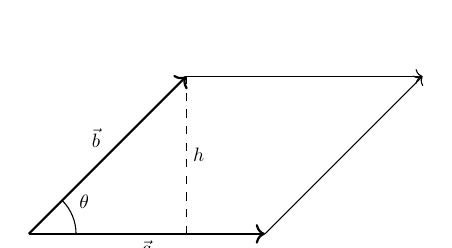
\begin{tikzpicture}[scale=1]
\draw[thick,->] (0,0) -- (3,0) node[pos=0.5, below,scale=0.7]{$\av$};
\draw[thick,->] (0,0) -- (2,2) node[pos=0.5, above left,scale=0.7]{$\bv$};
\draw[->] (3,0) -- (5,2) ;
\draw[->] (2,2) -- (5,2) ;
\draw[]  (0.6,0) arc (0:45:0.6) node[pos=0.5, above right, scale=0.7]{$\theta$};
\draw[dashed] (2,0) -- (2,2) node[pos=0.5, right,scale=0.7]{$h$};
\end{tikzpicture}
\end{center}



In $\FR^3$, on the other hand, three vectors $\av, \bv, \cv$ generically define a parallelepiped, as shown below. If one of the vectors is linearly dependent on the other two in will be coplanar with them and the parallelepiped will collapse to have zero volume. It is harder to picture in higher dimensions, but the idea is the same.

\begin{center}
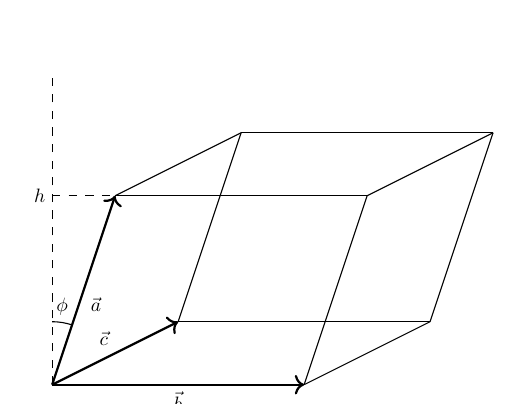
\begin{tikzpicture}[scale=0.8]
\draw[thick,->] (0,0) -- (1,3) node[pos=0.5, below right,scale=0.7]{$\av$};
\draw[thick,->] (0,0) -- (4,0) node[pos=0.5, below,scale=0.7]{$\bv$};
\draw[thick,->] (0,0) -- (2,1) node[pos=0.5, above left,scale=0.7]{$\cv$};
\draw[-] (4,0) -- (6,1) ;
\draw[-] (2,1) -- (6,1) ;

\draw[-] (1,3) -- (5,3) ;
\draw[-] (1,3) -- (3,4) ;
\draw[-] (5,3) -- (7,4) ;
\draw[-] (3,4) -- (7,4) ;

\draw[-] (4,0) -- (5,3) ;
\draw[-] (2,1) -- (3,4) ;
\draw[-] (6,1) -- (7,4) ;

\draw[dashed] (0,0) -- (0,5);
\draw[dashed] (0,3) -- (1,3) node [pos=0, left,scale=0.7]{$h$};
\draw[]  (0,1) arc (90:71.56:1) node[pos=0.5, above, scale=0.7]{$\phi$};
\end{tikzpicture}
\end{center}



\begin{example}{}
Using a determinant to test for a basis of $\FR^3$:


Let
\[
\vv_1=\begin{pmatrix}1\\0\\2\end{pmatrix},\qquad
\vv_2=\begin{pmatrix}0\\1\\-1\end{pmatrix},\qquad
\vv_3=\begin{pmatrix}3\\2\\1\end{pmatrix}.
\]
Form the associated matrix with these vectors as columns:
\[
A:=\left(\begin{array}{c|c|c}
\vv_1 & \vv_2 & \vv_3
\end{array}\right)
=
\begin{pmatrix}
1 & 0 & 3\\
0 & 1 & 2\\
2 & -1 & 1
\end{pmatrix}.
\]
Compute its determinant (expand along the first row, for example):
\[
\det(A)
=
1\cdot
\det\begin{pmatrix}1&2\\-1&1\end{pmatrix}
-0\cdot(\cdots)
+3\cdot
\det\begin{pmatrix}0&1\\2&-1\end{pmatrix}.
\]
Hence
\[
\det(A)
=
\bigl(1\cdot 1 - 2\cdot(-1)\bigr)
+3\bigl(0\cdot(-1)-1\cdot 2\bigr)
=
(1+2)+3( -2)
=
3-6
=
-3\neq 0.
\]
Therefore, by the theorem,
\[
\vv_1,\vv_2,\vv_3 \text{ is a basis of } \FR^3.
\]
\end{example}

We can also use the determinant test  when the vectors do {\it not} form a basis:

\begin{example}{}
Using a determinant to test for a basis of $\FR^3$ (an example where the vectors don't form a basis).

Let
\[
\vv_1=\begin{pmatrix}1\\0\\2\end{pmatrix},\qquad
\vv_2=\begin{pmatrix}0\\1\\-1\end{pmatrix},\qquad
\vv_3=\begin{pmatrix}1\\1\\1\end{pmatrix}.
\]
(Notice that \(\vv_3=\vv_1+\vv_2\).)

Form the associated matrix with these vectors as columns:
\[
A:=\left(\begin{array}{c|c|c}
\vv_1 & \vv_2 & \vv_3
\end{array}\right)
=
\begin{pmatrix}
1 & 0 & 1\\
0 & 1 & 1\\
2 & -1 & 1
\end{pmatrix}.
\]
Compute its determinant (expand along the first row, for example):
\[
\det(A)
=
1\cdot
\det\begin{pmatrix}1&1\\-1&1\end{pmatrix}
-0\cdot(\cdots)
+1\cdot
\det\begin{pmatrix}0&1\\2&-1\end{pmatrix}.
\]
Hence
\[
\det(A)
=
\bigl(1\cdot 1 - 1\cdot(-1)\bigr)
+\bigl(0\cdot(-1)-1\cdot 2\bigr)
=
(1+1)+(-2)
=
0.
\]
Therefore, by the theorem,
\[
\vv_1,\vv_2,\vv_3 \text{ do not form a basis of } \FR^3.
\]
(In fact they are linearly dependent since \(\vv_3=\vv_1+\vv_2\).)

\end{example}


	\section{Vector Spaces in General}
    \label{sec:VectorSpace}
	
	 In the previous chapter, we introduced the space $\FR^n$ of \textit{vectors}. The key operations for vectors in $\FR^n$ are {\it adding} two vectors and {\it multiplying} a vector by a scalar.  In this section, we will develop the general abstract framework allowing us to treat various examples of vector spaces in a uniform way.
	
	
	\subsection{Examples and definition}
    \label{ssec:VSDefinition}
	

%	Here are some examples that will be used throughout the course: 
	
	
	To be able to treat  various cases with a single mathematical framework, we now introduce the notion of an \textit{abstract vector space}.  This is the notion that makes rigorous this idea of `spaces of objects where one can add vectors and multiply them by a scalar'.
	
	
	
	\begin{df}{}
    \index{vector space}\index{vector space axioms}\label{def:vectorspace}
		A \textit{real vector space}  is a set $V$ (whose elements are called \textit{vectors}) endowed with two operations:
		\begin{itemize}
			\item[(i)] an \textit{addition} denoted  $+$ that associates to two vectors $\uv,\vv\in V$ a vector $\uv + \vv\in V$,
			\item[(ii)] a \textit{multiplication by a scalar} denoted $\cdot$ that associates to a vector $\vv \in V$ and a scalar $\lambda \in \FR$ a vector $\lambda \cdot \vv \in V$ (or simply $\lambda \vv$).
		\end{itemize} 
	We further require that the following \textit{vector space axioms} are satisfied:
		\begin{itemize}
			\item[(1)] \textit{null vector:} There is an element $\nv=\nv_V\in V$, the \textit{zero} or \textit{null vector}, such that $\vv+\nv=\vv$ for all $\vv\in V$.
			\item[(2)] \textit{opposite:} For all $\vv\in V$, there is an element $-\vv\in V$ such that $\vv+(-\vv)=\nv$.
			\item[(3)] \textit{commutativity of the addition:}  $\vv+\wv=\wv+\vv$ for all $\vv,\wv\in V$,
			\item[(4)] \textit{associativity of the addition:}  $(\vv+\wv)+\uv=\vv+(\wv+\uv)$ for all $\vv,\wv,\uv\in V$.
			\item[(5)] \textit{distribituvity of the scalar multiplication:}  $a(\vv+\wv)=a\vv+a\wv$ and $(a+b)\vv=a\vv+b\vv$, $a,b\in \FR$, $\vv,\wv\in V$,
			\item[(6)] \textit{associativity of the scalar multiplication:} $a(b\vv)=(ab)\vv$, $a,b\in\FR$, $\vv\in V$,
			\item[(7)] \textit{compatibility:} $1\cdot\vv=\vv$.
		\end{itemize}
	\end{df}
	
	This list of axioms (1)-(7) may seem long and technical. However, you should convince yourself that they encode the usual properties that one expects from addition and multiplication by a number for vectors, functions, etc. Moreover, the strength of this abstract framework is that, once we know that something is a vector space, we can treat objects of that space (functions, sequences, or more exotic objects) as if they were vectors, and use our geometric intuition to solve problems. 
%	This is similar to the process where one ends up doing additions or multiplications with complex numbers,  as if they were real numbers, once we have realised that they satisfy the same `rules of arithmetic'.
	
	\begin{itemize}
		\item[(i)] The space $\FR^n$ is a  vector space for the addition and multiplication by a scalar introduced in the previous chapter. The null vector $(0, \ldots, 0)^T$ satisfies axiom (1). The opposite of a vector $(v_1, \ldots, v_n)^T$ is defined as $(-v_1, \ldots, -v_n)^T$ to satisfy axiom (2). One then checks that axioms (3)-(7) hold. Indeed, one has to check the equations coordinate by coordinate, and each of these equations then boils down to a standard rule about addition and multiplication of real numbers (commutativity of addition, distributivity of the multiplication, etc.)
		
		
		\item[(iii)] The space $\FR^\FN$ is a vector space for the addition and multiplication by a scalar defined above. Here, a vector is a sequence 
		$$\vecttt{u_0}{u_1}{\vdots},$$ the zero vector is the \textit{zero sequence} 
		$$\vecttt{0}{0}{\vdots},$$ and the opposite of a vector is given by 
		$$-\vecttt{u_0}{u_1}{\vdots}\coloneqq=  \vecttt{-u_0}{-u_1}{\vdots}.$$ Here again, one then checks that axioms (3)-(7) hold, by checking each equation pointwise. 
		
%		\item[(iv)] The space $\FC$ of complex numbers can be seen as a real vector space: vectors are complex numbers, the null vector is $0 \in \FC$, the opposite of a complex number $z$ is $-z$, etc. 
	\end{itemize}

\paragraph{Complex vector spaces.} We have just defined \textit{real} vector spaces, that is, vector spaces where the set of scalars is $\FR$. These will be the almost sole focus of this course. However, one can analogously define \textit{complex vectors spaces} by setting the set of scalars to be $\FC$ and having the same list of axioms. Examples of complex vectors spaces are: 
\begin{itemize}
	\item The space $\FC^n$ of vectors of the form $(z_1, \ldots, z_n)^T$ with $z_i \in \FC$ for every $i$.
	\item  The space $\CF(\FC)$ of functions from $\FC$ to $\FC$.
	\item  The space $\CP(\FC)$ of polynomial functions with complex coefficients.
	\item The space $\FC^\FN$ of complex sequences $(z_0, z_1, \ldots)$ with $z_i \in \FC$ for every $i \geq 0$.
\end{itemize}

	

	
	
	
	\subsection{Linear combinations  in abstract vector spaces}\label{ssec:2.3.Span}
	
	We now generalise to abstract vector spaces the notions we introduced in $\FR^n$.
	
	\begin{df}{}
    \index{linear combination}
		A vector $\vv\in V$ is called a \textit{linear combination} of the vectors $\uv_1,\ldots,\uv_k\in V$, if it can be written as
		\begin{equation*}
		\vv=a_1\uv_1+a_2\uv_2+\ldots+a_k\uv_k~,~~~a_1,\ldots,a_k\in\FR~.
		\end{equation*}
		This is an extension of our definition of linear combination of vectors in $\FR^n$.
	\end{df}
	
	\begin{example} Consider the vector space  $\CP_2(\FR)$ of polynomials of degree at most 2. Linear combinations of the two functions (=vectors) defined $P_1(x) = x$ and $P_2(x)= x^2$ are polynomial functions of the form $$a_1x+a_2 x^2, ~~\mbox{ for } a_1, a_2 \in \FR.$$
		For instance, the polynomial function defined $P(x) = 5x^2 - 2x$ is a linear combination of $x$ and $x^2$, since we have $P= 5P_2 - 2P_1$.
		\end{example}
	
	\begin{df}{}
    \index{span}
		The \textit{span} of a family of vectors $\uv_1,\ldots,\uv_k$, usually denoted by $span(\uv_1,$ $\ldots,\uv_k)$, is the set of all possible linear combinations of $\uv_1,\ldots,\uv_k$:
		\begin{equation*}
		span(\uv_1,\ldots,\uv_k) :=\{a_1\uv_1+\ldots+a_k\uv_k|a_1,\ldots,a_k\in\FR\}~.
		\end{equation*}
		We also say that $span(\uv_1,\ldots,\uv_k)$ is spanned by $\uv_1,\ldots,\uv_k$ or that these vectors span $span(\uv_1,\ldots,\uv_k)$.
	\end{df}
	
	\begin{example}
    \begin{itemize}
			\item[(i)] The vectors $(1,0,0)^T$, $(0,1,0)^T$, $(0,0,1)^T$ span $\FR^3$.
		\item[(ii)] The vector space of polynomials up to degree $n$, $\CP_n(\FR)$, is spanned by the polynomials $1,x,x^2,$ $\ldots,x^n$, as every polynomial function in $\CP_n(\FR)$ can be written as $a_0 \times 1 + \ldots + a_nx^n$.
		\item[(iii)] The polynomial function $2x^2 +x -1$ belongs to span$(x^2+x, x+1)$ since $2x^2+x-1 = 2(x^2 +x) - (x+1)$.
%		In the real vector space $\FC$,  every complex number can be written as $a+bi$ with $a, b \in \FR$. It follows that $\FC$ is spanned by $1$ and $i$.
\end{itemize}
		\end{example}
	
	%\eolec{3.2}{3.3}

		
			\begin{df}{}
            \index{linearly dependent}\index{linearly independent} We say that  vectors $\vv_1,\ldots,\vv_k$ are \textit{linearly independent} if 
			$$c_1\vv_1+\ldots+c_k\vv_k=\nv ~~\Longrightarrow ~~ c_1 = \ldots = c_k =0.$$
			Otherwise, we say that the vectors are \textit{linearly dependent}. This is an extension of our definition of linear independence for $\FR^n$. 
			%		there exist $c_1,\ldots,c_k\in\FR$ not all equal to zero such that $c_1\vv_1+\ldots+c_k\vv_k=\nv$. If the only solution to the system of linear equations $c_1\vv_1+\ldots+c_k\vv_k=\nv$ is the trivial solution $c_1=\ldots=c_k=0$, then the vectors are \textit{linearly independent}. We say that a set of vectors is linearly independent, if the vectors in the set are linearly independent. This is an extension of our definition of linear dependence for $\FR^n$.
		\end{df}
		
		As in the case of $\FR^n$, linear dependence as a simple interpretation: a family of vectors $\uv_1,\ldots,\uv_k$ is linearly dependent, if and only if one (i.e.\ at least one) of the $\uv_i$s can be expressed as a linear combination of the others.
	

		%\item The vector space of $2\times2$-dimensional matrices $\sMat_2$ is spanned by
		%\begin{equation*}
		% \left(\begin{array}{cc}1 & 0 \\ 0 & 0
		%       \end{array}\right)~,~~~
		%\left(\begin{array}{cc}0 & 1 \\ 0 & 0
		%       \end{array}\right)~,~~~
		%\left(\begin{array}{cc}0 & 0 \\ 1 & 0
		%       \end{array}\right)~,~~~
		%\left(\begin{array}{cc}0 & 0 \\ 0 & 1
		%       \end{array}\right)~.
		%\end{equation*}

	
%	
%	\begin{prop}\label{th:2.3.6} Suppose $\vv_1,\ldots \vv_k$ span $V$ and $\vv_1$ is a linear combination of $\vv_2,\ldots,\vv_k$. Then $\vv_2,\ldots,\vv_k$ span $V$.
%	\end{prop}
%	
%	
%	
%	\begin{proof}
%		Let $\vv\in V$. Since $\span\{\vv_1,\ldots,\vv_k\}=V$, there are constants $c_1,\ldots,c_k\in\FR$ such that $\vv=c_1\vv_1+c_2\vv_2+\ldots+c_k\vv_k$. Since $\vv_1$ is a linear combination of $\vv_2,\ldots,\vv_k$, there are constants $d_2,\ldots,d_k\in\FR$ such that $\vv_1=d_2\vv_2+\ldots+d_k\vv_k$. Hence:
%		\begin{equation*}
%		\vv=c_1(d_2\vv_2+\ldots+d_k\vv_k)+c_2\vv_2+\ldots+c_k\vv_k=(c_1d_2+c_2)\vv_2+\ldots+(c_1d_k+c_k)\vv_k~.
%		\end{equation*}
%		Thus, every vector $\vv\in V$ can be expressed as a linear combination of $\vv_2,\ldots,\vv_k$ and so $\vv_2,\ldots,\vv_k$ span $V$.
%	\end{proof}
%	
	
%	\paragraph{Spans and subspaces.}
%	
%	\begin{thm}
%		Let $U$ be a vector space, let $V$ be a vector subspace, and let $\vv_1, \ldots, \vv_k$ be vectors of $U$. Then we have:
%		$$\vv_1, \ldots, \vv_k \in V ~~ \Longrightarrow ~~ \mathrm{span}(\vv_1, \ldots, \vv_k) \subset V.$$
%		\end{thm}
	
%	\paragraph{A criterion for linear independence in abstract vector spaces.}\label{ssec:LinearDependence} Unlike in the case of $\FR^n$, there is no automatic recipe to show that a family of vectors is linearly independent. However, we present here a useful criterion that works in many situations. Such a criterion relies on a notion that will become crucial in the next chapter.
%	
%	
%	\begin{definition}
%		Let $U$ be a vector space and let $n \geq 1$. A \textit{linear map} from $U$ to $\FR^n$ is map 
%		$$T: U \rightarrow \FR^n$$
%		that is compatible with the vector space operations, that is:
%			\begin{itemize}
%			\item[(1)] $T(\uv+\vv)=T(\uv)+T(\vv)$ for all $\uv,\vv\in U$.
%			\item[(2)] $T(\lambda\uv)=\lambda T(\uv)$ for all $\lambda\in\FR$ and $\uv\in U$.
%		\end{itemize}
%		\end{definition}
%	
%	In a sense, a linear map is a map that is `compatible' with the structure of vector spaces. Indeed, each of the vector spaces $U$ and $\FR^n$ come with an addition and a scalar multiplication, and we want to focus on those maps that respect these operations: they send a sum to a sum and a scalar multiple to a scalar multiple. This is exactly what the definition of a linear map requires.
%	
%	\begin{example}
%		TBC??? Evaluation, differentiation, etc.
%		\end{example}
%	
%
%	
%	\begin{thm}
%		Let $U$ be a vector space, and let $n \geq 1$. Let $T: U \rightarrow \FR^n$ be a linear map. Let $\uv_1, \ldots, \uv_k$ be a family of vectors of $U$.
%		
%		If  $T(\uv_1), \ldots, T(\uv_k)$ is a linearly independent family of vectors of $\FR^n$, then $\uv_1, \ldots, \uv_k$ is a linearly independent family of vectors of $U$.
%		\end{thm}
%	
%	A particularly useful case is to consider a map from $U$ to $\FR^k$. Indeed, the family $T(\uv_1), \ldots, T(\uv_k)$  is linearly independent if and only if their determinant is non-zero, which is something relatively easy to check. Of course, the hard part is finding the right map $T$ in the first place...
%	
%
%	\begin{proof}
%		If the set is linearly dependent, then there are constants $c_1,\ldots,c_k$ not all vanishing such that $c_1\uv_1+\ldots+c_k\uv_k=\nv$. Assume that $c_i\neq 0$. We can then solve the equation for $\uv_i$:
%		\begin{equation*}
%		\uv_i=\frac{1}{c_i}(c_1\uv_1+\ldots+c_{i-1}\uv_{i-1}+c_{i+1}\uv_{i+1}+\ldots+c_k\uv_k)~.
%		\end{equation*}
%		Inversely, if $\uv_i$ can be expressed as a linear combination of the others, we can transform this equation into that demonstrating linear dependence.
%	\end{proof}
	
%	\begin{example}
%		\item[(i)] Recall that the vectors $(1,0)^T,(0,1)^T$ are linearly independent in $\FR^2$, as
%		\begin{equation*}
%		c_1\vectt{1}{0}+c_2\vectt{0}{1}=\nv~~\Rightarrow~~\vectt{c_1}{c_2}=\vectt{0}{0}
%		\end{equation*}
%		which implies $c_1=c_2=0$. Analogously, the vectors $(1,0,0)^T,(0,1,0)^T,(0,0,1)^T$ are linearly independent in $\FR^3$ and the generalisation to $\FR^n$ is clear.\\
%		\item[(ii)] The vectors of  $(1,2)^T,(2,4)^T \in \FR^2$ are linearly dependent, as $2(1,2)^T-(2,4)^T=\nv$.\\
%		\item[(iii)] Let $\uv_1=(1,-1,2)^T$, $\uv_2=(3,2,1)^T$, $\uv_3=(4,1,3)^T$. Then $\uv_1,\uv_2,\uv_3$ are linearly dependent as $\uv_3 = \uv_1+\uv_2$.
%	\end{example}

\begin{example}
	Let us show that the functions $f_1(x):=\cos(x), f_2(x):=\cos(2x), f_3(x):=\cos(3x)$ are linearly independent vectors of $\CF(\FR)$.
	
	
	Let $a, b, c\in \FR$ be scalars such that $af_1 + bf_2 + cf_3$ is the zero vector of $\CF(\FR)$, that is, the zero function. This is equivalent to: 
	$$ a\cos(x)+b \cos(2x) +c\cos(3x)=0 ~~~\mbox{ for every }~x\in \FR.$$
	By evaluating at $x= \pi/2$, we get $b=0$, hence $ a\cos(x) +c\cos(3x)=0 $ for every $x \in \FR$. By evaluating this equation at $x = \pi/6$, we get $a\times \sqrt{3}/2 = 0$, hence $a=0$. Finally, we have $c\cos(3x)=0$ for every $x \in \FR$, and evaluating at $x=0$ yields $c=0$. 
	
	We thus have $a=b=c=0$, and it follows that $f_1, f_2, f_3$ are linearly independent.
	
	\end{example}

%	\paragraph{Remark.} Unlike the case of vectors in $\FR^n$ where checking linear independence amounted to solving a system of linear equations, there is no automatic way to check that a family of functions is linearly independent. The previous example illustrates a powerful method: evaluating at different points to obtain several linear equations. You will see other manipulations in tutorials that allow you to check the linear independence of certain families of functions.
%	
%	\begin{method}{Determining whether vectors are linearly independent} To determine whether vectors $\{\uv_1,\ldots,\uv_k\}$ are linearly independent, one uses Gaussian elimination to find all solutions to the system
%	\begin{equation*}
%	c_1\uv_1+c_2\uv_2+\ldots+c_k\uv_k=\nv~.
%	\end{equation*}
%	If all variables $c_1,\ldots, c_k$ are pivot variables, this homogeneous system of linear equations has only the trivial solution $c_1=c_2=\ldots=c_k=0$. In this case, the set $\{\uv_1,\ldots\uv_k\}$ is linearly independent. Otherwise, nontrivial solutions exist and the vectors are linearly dependent.
%	\end{method}
%	
%	\begin{example} Let us determine whether the vectors $(1,2,3,-1)^T$, $(2,1,3,1)^T$ and $(4,5,9,-1)^T$ are linearly dependent. We must find all solutions $(c_1,c_2,c_3)$ of the homogeneous SLE
%	\begin{equation*}
%	c_1\left(\begin{array}{c}
%	1 \\ 2 \\ 3 \\ -1
%	\end{array}\right)+
%	c_2\left(\begin{array}{c}
%	2 \\ 1 \\ 3 \\ 1
%	\end{array}\right)+
%	c_3\left(\begin{array}{c}
%	4 \\ 5 \\ 9 \\ -1
%	\end{array}\right)=
%	\left(\begin{array}{c}
%	0 \\ 0 \\ 0 \\ 0
%	\end{array}\right)~.
%	\end{equation*}
%	That is, we have to analyse
%	\begin{equation*}
%	\begin{array}{ccccl}
%	c_1&+2c_2&+4c_3&=&0\\
%	2c_1&+c_2&+5c_3&=&0\\
%	3c_1&+3c_2&+9c_3&=&0\\
%	-c_1&+c_2&-c_3&=&0\\
%	\end{array}~~\rightsquigarrow~~
%	\left(\begin{array}{ccc|c}1 & 2 & 4 & 0 \\ 2 & 1 & 5 & 0 \\ 3 & 3 & 9 & 0 \\ -1 & 1 & -1 & 0\end{array}\right)
%	\end{equation*}
%	\begin{equation*}
%	\melt{R_2\rightarrow R_2-2R_1\\R_3\rightarrow R_3-3R_1\\R_4\rightarrow R_4+R_1}
%	\left(\begin{array}{ccc|c}1 & 2 & 4 & 0 \\ 0 & -3 & -3 & 0 \\ 0 & -3 & -3 & 0 \\ 0 & 3 & 3 & 0\end{array}\right)
%	\melt{R_3\rightarrow R_3-R_2\\R_4\rightarrow R_4+R_3\\R_2\rightarrow -\frac{1}{3}R_2}
%	\left(\begin{array}{ccc|c}1 & 2 & 4 & 0 \\ 0 & 1 & 1 & 0 \\ 0 & 0 & 0 & 0 \\ 0 & 0 & 0 & 0\end{array}\right)~.
%	\end{equation*}
%	Not all the variables are pivot variables ($c_3$ is a free variable) and therefore the system has infinitely many solutions, which implies that the vectors are linearly dependent. More precisely, if we rewrite it as a system of linear equations, we get
%	\begin{equation*}
%	\begin{array}{rcl}
%	c_1+2c_2+4c_3&=&0\\
%	c_2+c_3&=&0\\
%	\end{array}~~~
%	\begin{array}{l}
%	\rightarrow c_1=-2c_2-4c_3=-2\alpha\\
%	\rightarrow c_3=\alpha\Rightarrow c_2=-\alpha\\
%	\end{array}~~~.
%	\end{equation*}
%	Putting $\alpha=1$, for example, we obtain
%	\begin{equation*}
%	-2\left(\begin{array}{c}
%	1 \\ 2 \\ 3 \\ -1
%	\end{array}\right)-
%	\left(\begin{array}{c}
%	2 \\ 1 \\ 3 \\ 1
%	\end{array}\right)+
%	\left(\begin{array}{c}
%	4 \\ 5 \\ 9 \\ -1
%	\end{array}\right)=
%	\left(\begin{array}{c}
%	0 \\ 0 \\ 0 \\ 0
%	\end{array}\right)~.
%	\end{equation*}
%	\end{example}
	
%	\begin{remark}\label{rem:2.4.5} 
%		\item[(i)] Two vectors $\uv_1,\uv_2$ are linearly dependent if and only if $\uv_2=\nv$ or $\uv_1$ is a multiple of $\uv_2$. The first case is clear, as $c_1\uv_1+c_2\nv=\nv$ has nontrivial solutions such as $c_1=0$, $c_2=1$. In the second case, assume that $\uv_1=\lambda \uv_2$, then $c_1\uv_1+c_2\uv_2=\nv$ has the nontrivial solutions $c_1=\alpha$, $c_2=-\lambda\alpha$, $\alpha\in\FR$.\\
%		\item Let $\{\vv_1,\ldots,\vv_k\}$ be a set of vectors in $\FR^n$ with $k>n$. Then $c_1\vv_1+\ldots+c_k\vv_k=\nv$ gives rise to a homogeneous system of linear equations with $n$ equations in $k$ unknowns. As $k>n$, this system must have a non-zero solution (Theorem  \ref{th:1.4.3}) and therefore $\vv_1,\ldots,\vv_k$ are linearly dependent.
%	\end{remark}
%	
%	
%	
%	
%	\paragraph{Theorem.}\label{th:2.4.6} Suppose $\{\vv_1,\ldots,\vv_k\}$ is linearly independent and $\vv_0\notin\span\{\vv_1,\ldots,\vv_k\}$. Then $\{\vv_0,\vv_1,\ldots,\vv_k\}$ is linearly independent.
%	\begin{proof}
%		Suppose $c_0\vv_0+c_1\vv_1+\ldots+c_k\vv_k=\nv$. If $c_0\neq 0$, $\vv_0=-\frac{1}{c_0}(c_1\vv_1+\ldots+c_k\vv_k)$ and so $v_0\in\span\{\vv_1,\ldots,\vv_k\}$, which we know is not the case. Thus, $c_0=0$. But we know that $\{\vv_1,\ldots,\vv_k\}$ are linearly independent, and so the only solution to the SLE $c_0\vv_0+c_1\vv_1+\ldots+c_k\vv_k=c_1\vv_1+\ldots+c_k\vv_k=\nv$ is $c_0=c_1=\ldots=c_k=0$. Therefore, $\{\vv_0,\vv_1,\ldots,\vv_k\}$ is linearly independent.
%	\end{proof}
%	
%	%\tut{4}
	%\end{tutsectionthree}
	%\begin{tutsectionfour}
	
	\subsection{Basis and dimension}\label{ssec:BasisDimension}
	
	%\paragraph{Basis of a vector space.}
	
	\begin{df}{}
  %  \index{basis}
	A family of vectors
%		\footnote{The round brackets $(\ldots)$ denote a tuple which is an ordered list of elements. A set, denoted by curly brackets $\{\ldots\}$, is a list of elements without any order. In particular $\{a,b\}=\{b,a\}$, while $(a,b)\neq(b,a)$ if $b\neq a$.} 
		$\uv_1,\ldots,\uv_n$ is called a \textit{basis} of $V$, if it  is a linearly independent set of vectors that span $V$.
		
%		A vector space if \textit{finite dimensional} if it has a basis consisting of finitely many vectors, and \textit{infinite dimensional} otherwise.
	\end{df}
	
	%\eolec{3.3}{4.1}
	
	\begin{example}
    \label{ex:2.5.2}
	We have already seen the standard basis $\ev_1 = (1, 0, \ldots, 0)^T$, $\ldots$ ,$ \ev_n = (0, \ldots, 0, 1)^T$ of $\FR^n$. 

		Note that a real vector space has infinitely many bases. For instance, $(1, 1)^T$ and $(1, -1)^T$ is also a basis of $\FR^2$ {Why?}. 

	\end{example}

 Here is an important example:
\begin{thm}{}
\label{thm:basis_pol}
A basis for the vector space of polynomials of degree at most $n$ is $1,x,x^2,\ldots,x^n$.
	\end{thm}

\begin{proof}
	The family clearly spans $\CP_n(\FR)$, as every polynomial function of $\CP_n(\FR)$ can be written as a linear combination $a_0 + a_1x + \ldots + a_n x^n$ for some scalars $a_0, \ldots, a_n \in \FR$.
	Let us show that this family is free. Suppose that we have a linear combination $a_0 + a_1x + \ldots + a_n x^n$ that is the zero vector, that is, $a_0 + a_1x + \ldots + a_n x^n= 0$ for every $x\in \FR$. By evaluating at $x=0$, we get $a_0 = 0$. Now since the polynomial function $a_0 + a_1x + \ldots + a_n x^n$ is the zero function, so its derivative, so we get $a_1 + 2a_2x + \ldots + na_nx^{n-1} = 0$ for every $x \in \FR$. Evaluating again at $x=0$, we get $a_1 = 0$. By repeating the same procedure (differentiating and evaluating at $x=0$), we prove successively that $a_0 = a_1 = \ldots = a_n = 0$. Thus, the family of polynomial functions $1, x, \ldots, x^n$ is linearly independent, so it is a basis of  $\CP_n(\FR)$.
\end{proof}



	\subsection{Dimension of a vector space.} 
    In order to define the dimension of a vector space, we need the following important result: 
	
		\begin{thm}{}
        \label{th:2.5.4} Any two bases for a vector space $V$ contain the same number of vectors.
	\end{thm}

Before proving it, we need the following result:
	
	\begin{thm}{}
    \label{lem:2.5.3} If a family of vectors $\vv_1,\vv_2,\ldots,\vv_n$ is a basis of a vector space $V$, then every family of vectors of $V$ containing more than $n$ vectors is linearly dependent.
		\end{thm}
	\begin{proof}
		Let $\wv_1,\wv_2,\ldots,\wv_m$ be a family of $m>n$ vectors of $V$. We will show that there exist $c_1,c_2,\ldots,c_m$ not all zero such that
		\begin{equation}\label{eq:SLE1}
		c_1\wv_1+c_2\wv_2+\ldots+c_m\wv_m=\nv~.
		\end{equation}
		Since $\vv_1,\vv_2,\ldots,\vv_n$ spans $V$, each $\wv_i$ can be expressed as a linear combination of the $\vv_i$'s:
		\begin{equation*}
		\begin{aligned}
		\wv_1&=a_{11}\vv_1+a_{12}\vv_2+\ldots+a_{1n}\vv_n~,\\
		\wv_2&=a_{21}\vv_1+a_{22}\vv_2+\ldots+a_{2n}\vv_n~,\\
		\vdots & \hspace{2cm}\vdots\\
		\wv_m&=a_{m1}\vv_1+a_{m2}\vv_2+\ldots+a_{mn}\vv_n~.
		\end{aligned}
		\end{equation*}
		Plugging this into \eqref{eq:SLE1}, we have
		\begin{equation*}
		c_1(a_{11}\vv_1+\ldots+a_{1n}\vv_n)+\ldots+c_m(a_{m1}\vv_1+\ldots+a_{mn}\vv_n)=\nv~.
		\end{equation*}
		To have all the coefficients of the $\vv_1,\ldots,\vv_n$ vanish, note that it is sufficient to find $c_1,\ldots,c_m$ such that
		\begin{equation*}
		\begin{aligned}
		a_{11}c_1+a_{21}c_2+\ldots+a_{m1}c_m &=0~,\\
		a_{12}c_1+a_{22}c_2+\ldots+a_{m2}c_m &=0~,\\
		\vdots\hspace{2cm}&\vdots\\
		a_{1n}c_1+a_{2n}c_2+\ldots+a_{mn}c_m &=0~.
		\end{aligned}
		\end{equation*}
		This is a homogeneous system of linear equations with more unknowns ($m$) than equations ($n$) and thus there is a solution with not all of the $c_i$ being zero. It follows that \eqref{eq:SLE1} has a solution besides the trivial solution and so $S'$ is linearly dependent.
	\end{proof}
	

	\begin{proof}[Proof of Proposition \ref{th:2.5.4}]
		Let $B=(\vv_1,\vv_2,\ldots,\vv_n)$ and $B'=(\vv'_1,\vv'_2,\ldots,\vv'_m)$ be bases for $V$. From the above lemma, we conclude that since $B$ is a basis and $B'$ is linearly independent, $m\leq n$. Equally, since $B'$ is a basis and $B$ is linearly independent, $n\leq m$. Altogether, we have $m=n$.
	\end{proof}
%	
%	\paragraph{Remark.} From lemma \ref{lem:2.5.3} and theorem \ref{th:2.5.4}, it follows that a basis for $V$ contains a minimal number of vectors that span $V$, but a maximal number of vectors that are still linearly independent.
	
	We are now able to define properly the dimension of a vector space: 
	
	\begin{thm}{}
    \index{dimension}
		Let $V$ be a vector space. We say that $V$ is \textit{finite-dimensional} if it has a finite basis, and \textit{infinite-dimensional} otherwise. We define the \textit{dimension} of $V$ to be the number of vectors in any basis of $V$.
	\end{thm}


	
	\begin{example}
	We have constructed bases of several vector spaces. We  have the following dimensions:
		\begin{equation*}
		\begin{tabular}{r|c|c|c|c}
		Space & $\FR^2$  & $\FR^3$ & $\FR^n$ & $\CP_n(\FR)$ \\
		\hline
		Dimension & 2 & 3 & $n$ & $n+1$ 
		\end{tabular}
		\end{equation*}
%		\item[(ii)] Consider the straight line $L=\{(x,y,z)^T:\frac{x}{2}=\frac{y}{3}=\frac{z}{5}\}$. If $(x,y,z)^T\in L$, then $\frac{x}{2}=\frac{y}{3}=\frac{z}{5}=\alpha$ for some $\alpha\in\FR$ and therefore $(x,y,z)^T=\alpha(2,3,5)^T$ and $L=\{\alpha(2,3,5)^T:\alpha\in\FR\}=\span\{(2,3,4)^T\}$. Since a single non-zero vector is always linearly independent, $\big((2,3,5)^T\big)$ is a basis for $L$ and we have $\dim L=1$.\\
%		\item[(iii)] Consider the plane $P=\{(x,y,z)^T\in\FR^3:x+y-z=0\}$. Then $P$ is a subspace of $\FR^3$. Consider the vectors $(1,0,1)^T,(0,1,1)^T$ of $P$. Since $(1,0,1)^T$ and $(0,1,1)^T$ are not multiples of each other, they are  linearly independent. Furthermore, they span $P$, since a vector of $P$ is of the form $(x,y,x+y)^T$ for some $x, y \in \FR$ and we have  $(x,y,x+y)^T=x(1,0,1)^T+y(0,1,1)^T$. We conclude that $(1,0,1)^T,(0,1,1)^T$ form a basis for $P$, and $P$ has dimension 2.\\
\end{example}

The following result is useful in finding a lower bound for the dimension of a vector space:

\begin{thm}{}
	Let $V$ be a vector space, and let $\vv_1, \ldots, \vv_k$ be a linearly independent family. Then we have: $$\dim V \geq k.$$
\end{thm}








	
\subsection{Vector subspaces}\label{ssec:VectorSubspaces}

The previous examples are the main sources of vectors spaces for this course. However, we are often not interested in the space of all vectors, or of all functions. Instead, we are often interested in particular subsets of elements that satisfy some equation: system of linear equations, differential equations, etc. 

In this section, we introduce the notion of \textit{vector subspace} as the natural notion of subset of a vector space that is compatible with the operations of addition and multiplication by a scalar. We will see that the set of solutions of various equations naturally form a vector subspace of the associated vector space.

\begin{df}{}
Let $V$  be a vector space and let $W$ be a subset of $V$. We say that $W$ is a \textit{vector subspace}  (or simply a subspace) of $V$ if the following holds:
	
	\begin{itemize}
		\item[(i)] $\nv \in W$,
		\item[(ii)] for all $\wv_1,\wv_2\in W$, we have $\wv_1+\wv_2\in W$ and
		\item[(iii)] for all $\lambda\in\FR$ and $\wv\in W$, we have $\lambda \wv\in W$.
	\end{itemize}
	%		Equivalently, a vector subspace is a non-empty subset that is stable under linear combinations.
\end{df}



	A vector subspace $W$ of $V$ is itself a vector space, when endowed with the addition and scalar multiplication coming from $V$. (This is actually an equivalence: a subset $W$ is a subspace if and only if it $W$ is a vector space when endowed with the addition and scalar multiplication from $V$.)
	
	As a consequence, we can talk of the dimension or of bases of a  given subspace.


\begin{example}
\label{ex:2.2.2} 
\begin{itemize}
	\item[(i)] In a vector space $V$, the whole space $V$  and the trivial subset $\{\nv\}$ are always vector subspaces.
	\item[(ii)] Consider the subset $W=\{(x,y)^T\in\FR^2:x+y=0\}$ of $\FR^2$. That is, $W$ consists of all the vectors of the form $(x, -x)^T$ for $x \in \FR$. The null vector $(0,0)^T$ is clearly in $W$.  If we add two vectors or multiply a vector by a scalar in $W$, we end up back in $W$:
	\begin{equation*}
	\vectt{x_1}{-x_1}+\vectt{x_2}{-x_2}=\vectt{x_1+x_2}{-(x_1+x_2)}~~~\mbox{and}~~~\lambda\vectt{x_1}{-x_1}=\vectt{\lambda x_1}{-\lambda x_1}~.
	\end{equation*}
	Thus, $W$ us a subspace of $\FR^2$. Note that every vector of $W$ is of the form 
	$$\vectt{x}{-x} = x\vectt{1}{-1} ~~ \mbox{ for some } x \in \FR,$$
	so $W$ has dimension $1$ and a basis of $W$ is given by the vector $(1, -1)^T.$
    \end{itemize}
\end{example}

\paragraph{Remark.} 
%Here are immediate properties of vector subspaces:  \begin{itemize}\item[(i)] If $W$ is a vector subspace of $V$, then $W$ contains the null vector. Indeed, $W$ contains a vector $\wv$ as it is non-empty, and as $W$ is stable under multiplication by a scalar, it also contains $0.\wv = \nv$. \\
If a subspace $W$ contains a vector $\wv$, it also contains its opposite $-\wv$, as $W$ is stable under multiplication by a scalar and $-\wv = (-1).\wv$.
%\end{itemize}




\begin{example}\label{ex:2.2.2} 
	The subset $W'=\{(x,y)^T |  x+y=1\}$ is not a vector subspace of $\FR^2$, as $\nv=(0,0)^T$ is not an element of $W'$. Another reason is that the sum of two elements $w_1,w_2\in W'$ is not always in $W'$. For instance, $(1,0)^T$ and $(0,1)^T$ belong to $W'$, but their sum $(1,1)^T$ does not.
\end{example}


%\begin{thm}\index{vector subspace test} {\em (Vector subspace test)} Let $V$  be a vector space and let $W$ be a non-empty subset of $V$. Then $W$ is a vector subspace of $V$ iff (if and only if)
%\begin{itemize}
% \item[(i)] for all $\wv_1,\wv_2\in W$, we have $\wv_1+\wv_2\in W$ and
% \item[(ii)] for all $\lambda\in\FR$ and $\wv\in W$, we have $\lambda \wv\in W$.
%\end{itemize}
%\end{thm}
%\begin{proof}
%First, note that due to (i) and (ii), the restrictions of the operations $+$ and $\cdot$ from $V$ to $W$ are indeed well defined on $W$ and do not take us out of this set. It remains to check the vector space axioms. In the tutorials, we will show that $(-1)\vv=-\vv$ for any $\vv\in V$. We have already shown in \ref{ssec:VSDefinition}, \ref{th:vanishing} that $0\wv=\nv$. Take an arbitrary vector $\vv\in W$. Because of (ii), both $0\wv=\nv$ and $(-1)\vv=-\vv$ are also in $W$. Axiom (1) and (2) are therefore satisfied: There is a null vector $\nv$ in $W$, and every vector $\vv$ has an inverse $-\vv$ in $W$. The validity of the remaining axioms (3)-(7) is then inherited from $V$.
%\end{proof}

\begin{example}
\begin{itemize}
	\item[(i)] Let $V=\FR^2$. Then $W=\{(x,y)^T | x=3y\}$ is a vector subspace, since vectors of $W$ are of the form 
	$$\vectt{3y}{y} = y \vectt{3}{1} ~~ \mbox{ for some } y\in \FR,$$
	 and we have:
	\begin{equation*}
	\vectt{3y_1}{y_1}+\vectt{3y_2}{y_2}=\vectt{3(y_1+y_2)}{y_1+y_2}~~~\mbox{and}~~~\lambda\vectt{3y}{y}=\vectt{3\lambda y}{\lambda y}~,~~~\lambda\in\FR~.
	\end{equation*}
	Thus, $W$ is a subspace of $\FR^2$ of dimension $1$, and a basis of it is given by the vector $(3, 1)^T$.

	In general, lines through the origin of $\FR^2$ form vector subspaces of $\FR^2$.\\
	\item[(ii)] Lines in $\FR^2$ that do not pass through the origin do not contain $\nv$ and thus are not vector subspaces of $\FR^2$, cf.\ example in \ref{ex:2.2.2}.
    \end{itemize}
\end{example}



\paragraph{Subspaces of $\FR^2$.} We have seen already that we can completely describe the subspaces of $\FR^2$: 
\begin{itemize}
		\item[(i)] the trivial subspace $\{\nv \}$,
		\item[(ii)] lines through the origin,
		\item[(iii)] the whole space $\FR^2$.
	\end{itemize}
There is a similar picture in $\FR^3$, where subspaces can be lines through the origin, planes through the origin, etc. Geometrically, being stable under addition and scalar multiplication makes vector subspaces `look flat'.





\paragraph{Solutions of systems of linear differential equations as subspaces.}  We saw in a previous example how the set of solutions of certain differential equations may be described as a span, and hence is a subspace of $\CF(\FR)$. Even without an explicit description of the solutions, it is possible to show that the set of solutions forms a subspace. 


	Consider the following differential equation (linearised simple pendulum): 
$$ y'' + \omega^2 y=0.$$
Then the set $W$ of solutions of this equation is a subspace of $\CF(\FR)$.


\begin{proof}
	Let $y_1, y_2\in W$ and $\lambda\in \FR$. Then:
	\begin{equation*}
	\begin{aligned}
	&(y_1 + y_2)'' + \omega^2 (y_1 + y_2) =(y_1'' + \omega^2 y_1) + (y_2'' + \omega^2 y_2) = 0 + 0 = 0,\mbox{ hence } y_1+y_2\in W\\
	&(\lambda y_1)'' + \omega^2 (\lambda y_1) = \lambda(y_1'' + \omega^2 y_1) = \lambda 0 = 0,\mbox{ hence } \lambda y_1\in W~.
	\end{aligned}
	\end{equation*}
	We conclude that $W$ is a vector subspace of $\CF(\FR)$.
\end{proof}

%You have probably seen in a course on linear differential equations that $W$ consists of functions of the form $x \mapsto a \cos(\omega x) + b\sin(\omega x)$ for some constants $a, b \in \FR$. Using this description provides another way to check that $W$ is a vector subspace (Do it!).
	
	

	
%	Former proofs:
%		
%	\paragraph{From a spanning family to a basis.} 
%	
%	\begin{prop}\label{prop:span_removal}
%		Let $\uv_1, \ldots, \uv_k$ be a spanning family of $\FR^n$. If $\uv_k$ is a linear combination of $\uv_1, \ldots, \uv_{k-1}$, then $\uv_1, \ldots, \uv_{k-1}$ is also a spanning family.
%	\end{prop}
%	
%	\begin{proof}
%		Write $\uv_k = a_1 \uv_1 + \ldots + a_{k-1}\uv_{k-1}$ for some $a_1, \ldots, a_{k-1} \in \FR$. Then we have for every $\lambda_1, \ldots, \lambda_k \in \FR$:
%		\begin{equation*}
%		\begin{aligned}
%		\lambda_1 \uv_1 + \ldots + \lambda_k \uv_k &= \lambda_1 \uv_1 + \ldots + \lambda_{k-1} \uv_{k-1} + \lambda_k (a_1 \uv_1 + \ldots + a_{k-1}\uv_{k-1})\\
%		&= (\lambda_1 + a_1\lambda_k)\uv_1 + \ldots + (\lambda_{k-1}+a_{k-1}\lambda_k)\uv_{k-1}.
%		\end{aligned}
%		\end{equation*}
%		Since every vector of $\FR^n$ is a linear combination of $\uv_1, \ldots, \uv_k$ by assumption, it is also a linear combination of $\uv_1, \ldots, \uv_{k-1}$ by the previous computation.
%	\end{proof}
%	
%	
%	\begin{prop}
%		Let $\uv_1, \ldots, \uv_k$ be a spanning family. Then one can extract a subfamily that is a basis of $\FR^n$.
%	\end{prop}
%	
%	\begin{proof}
%		A minimal subfamily of $\uv_1, \ldots, \uv_k$ that still spans $\FR^n$ is necessarily linearly independent. Indeed, if it were linear dependent, one of its elements could be expressed in terms of the others, and Proposition \ref{prop:span_removal} would imply that we could remove that element and still span $\FR^n$, contradicting minimality.
%	\end{proof}
%	
%	\paragraph{From a linearly independent family to a basis.} 
%	
%	\begin{prop}\label{prop:ind_adding} Let $\uv_1, \ldots, \uv_k$ be a linearly independent family. If $\uv$ is a vector of $\FR^n$ that is not a linear combination of $\uv_1, \ldots, \uv_k$, then $\uv_1, \ldots, \uv_k, \uv$ is  also linearly independent.
%	\end{prop}
%	
%	\begin{proof}
%		Let $\lambda_1, \ldots, \lambda_k, \lambda \in \FR$ such that 	$\lambda_1\uv_1 + \cdots + \lambda_k\uv_k + \lambda \uv = \nv$. Since $\uv$ is  not a linear combination of $\uv_1, \ldots, \uv_k$, we have $\lambda = 0$, hence 	$\lambda_1\uv_1 + \cdots + \lambda_k\uv_k  = \nv$. Since $\uv_1, \ldots, \uv_k$ are linearly independent, it follows that $\lambda = \ldots = \lambda_k = 0$. 
%	\end{proof}
%	
%	\begin{prop}
%		Let $\uv_1, \ldots, \uv_k$ be a linearly independent family. Then one can extend it to a basis of $\FR^n$.
%	\end{prop}
%	
%	\begin{proof}
%		If $\uv_1, \ldots, \uv_k$ is already spanning, there is nothing to do. Otherwise, there exists a vector $\uv_{k+1} \notin \mathrm{span}(\uv_1, \ldots, \uv_k)$. By Proposition \ref{prop:ind_adding}, the family $\uv_1, \ldots, \uv_k, \uv_{k+1}$ is also linearly independent. We can repeat the procedure. Since a linearly independent family contains at most $n$ vectors by Proposition \ref{prop:ind_at_most}, this algorithm eventually stops, at which point we have that the resulting family $\uv_1, \ldots, \uv_m$ is still linearly independent and spans $\FR^n$, hence it is a basis.
%	\end{proof}
	
	
	
	%\paragraph{Remark.} The original vectors in the above example are linearly dependent. It follows from the matrix after the first set of elementary row operations that
	%\begin{equation*}
	% R_2-2R_1=R_3-4R_1~~~\mbox{or}~~~(2,-1,2,1)^T-2(1,2,-1,3)^T=(4,3,0,7)^T-4(1,2,-1,3)^T~.
	%\end{equation*}
	%
	%%\eolec{4.1}{4.2}
	
%	\begin{prop}\label{th:2.5.10} Let $V$ be an $n$-dimensional vector space and let $\vv_1,\ldots,\vv_k$ be a linearly independent family of vectors. Then $\vv_1,\ldots,\vv_k$ can be extended to a basis  $\vv_1, \ldots, \vv_n$ of $V$.\qed
%	\end{prop}
%%	\begin{proof}
%%		(by construction) Since $\span\{\vv_1,\ldots,\vv_k\}\neq V$, there is a $\vv_{k+1}\in V$ such that $\vv_{k+1}\notin\span\{\vv_1,\ldots,\vv_k\}$. By theorem \ref{ssec:LinearDependence}, \ref{th:2.4.6}, the set $\{\vv_1,\ldots,\vv_k,\vv_{k+1}\}$ is linearly independent. If $\span\{\vv_1,\ldots,\vv_k,\vv_{k+1}\}=V$, then we found a basis. Otherwise, we repeat this procedure. In each step, the dimension of the span of the vectors increases by one, and after $n-k$ steps, we arrive at the desired basis.
%%	\end{proof}
%
%
%
%	
%	\begin{prop}\label{th:2.5.11} Suppose that a family $\vv_1,\ldots,\vv_k$ of vectors spans a (finite-dimensional) vector space $V$. Then there exists a subfamily that is a basis for $V$.\qed
%	\end{prop}
%	\begin{proof}
%		(by construction) If $S$ is linearly independent, then $S$ is a basis. Otherwise, one of the $\vv_i$ can be written as a linear combination of the others as follows from lemma \ref{ssec:LinearDependence}, \ref{lem:3.4.6}. Therefore $S\backslash\{\vv_i\}$ still spans $V$ by theorem \ref{ssec:2.3.Span}, \ref{th:2.3.6}. We continue with this reduced set from the top as often as possible. The minimal set, which still spans $V$ is the basis of $V$.
%	\end{proof}
	

%	\begin{proof}
%		(i) (by contradiction) Assume that $S$ is not a basis for $V$. Then it can be extended to a basis by theorem \ref{th:2.5.10} with more than $n$ elements. This contradicts the assumption that $\dim V=n$.\\
%		(ii) Theorem \ref{th:2.5.11} tells us that a subset of $S$ spans $V$. Because $\dim V=n$, this subset has to have $n$ elements. So the subset of $S$ is all of $S$.
%	\end{proof}
	
%	\paragraph{Remark.} Note that we worked above with {\em finite dimensional} vector spaces.  For the complications in the case of infinite dimensional vector spaces and some strange features appearing in set theory, have a look at the \hyperref{http://en.wikipedia.org/wiki/Zorn's_lemma}{}{}{Wikipedia entry} for {\em Zorn's Lemma}.
%	



\paragraph{Dimension of subspaces.}

Since a subspace of vector space is itself a vector space, it also has a dimension. It is natural to wonder whether the dimension behaves well with respect to subspaces: For instance, is the dimension of a subspace at most the dimension of the original vector space? While this intuitively obvious, it requires a proof. And indeed, things go extremely well:  


\begin{thm}{}
\label{thm:sub_inclusion_dim}
	Let $V$ be a finite-dimensional vector space, and let $W$ be a subspace. Then 
	$$\dim W \leq \dim V.$$ Moreover, we have 
	$$\dim W = \dim V ~~ \Longleftrightarrow ~~ W = V.$$
\end{thm}
	%\tut{5}
	%\end{tutsectionfour}
	%\begin{tutsectionfive}
	
	This result can provide a simple way to show the equality between two subspaces: Instead of showing both inclusions, it is only necessary to show one inclusion and the equality of dimensions, something that is generally easier to handle. We will see applications in the next chapter.
	
	The previous theorem relies on the following results: 
	
		Let $V$ be an $n$-dimensional vector space and let $\vv_1,\ldots,\vv_k$ be a linearly independent family of vectors. Then $\vv_1,\ldots,\vv_k$ can be extended to a basis  $\vv_1, \ldots, \vv_n$ of $V$.\qed
	
	%	\begin{proof}
	%		(by construction) Since $\span\{\vv_1,\ldots,\vv_k\}\neq V$, there is a $\vv_{k+1}\in V$ such that $\vv_{k+1}\notin\span\{\vv_1,\ldots,\vv_k\}$. By theorem \ref{ssec:LinearDependence}, \ref{th:2.4.6}, the set $\{\vv_1,\ldots,\vv_k,\vv_{k+1}\}$ is linearly independent. If $\span\{\vv_1,\ldots,\vv_k,\vv_{k+1}\}=V$, then we found a basis. Otherwise, we repeat this procedure. In each step, the dimension of the span of the vectors increases by one, and after $n-k$ steps, we arrive at the desired basis.
	%	\end{proof}

	
	Suppose that a family $\vv_1,\ldots,\vv_k$ of vectors spans a (finite-dimensional) vector space $V$. Then there exists a subfamily that is a basis for $V$.\qed
	
	

\section{The solution space of a homogeneous system of linear equations.}

In F17ZB we looked at solving $A \xv = \bv$, now we are going to look in more detail at solving
the {\it homogeneous} system of equations
\[
A \xv = \nv
\]
This leads on naturally to a discussion of {\it rank} for matrices (we have already seen one definition of this in F17ZB).

\begin{thm}{}
\label{thm:hom_subspace} 
	The set of solutions  of a \textit{homogeneous} system of linear equations in $n$ unknowns is a vector subspace of $\FR^n$ whose dimension  is the number of free variables, after reducing the system to its echelon form.
	\end{thm}



\begin{proof}
 	Let $W$ be the set of solutions. By definition, we have $W= \{\xv \in \FR^n ~|~ A\xv = \nv\}$ for some matrix $A$. In particular, the null vector belongs to $W$. Let $\xv_1,\xv_2\in W$ and $\lambda\in \FR$. We have:
 \begin{equation*}
 \begin{aligned}
 &A(\xv_1+\xv_2)=A\xv_1+A\xv_2=\nv+\nv=\nv,\mbox{ hence } \xv_1+\xv_2\in W\\
 &A(\lambda \xv_1)=\lambda A\xv_1=\lambda\nv=\nv,\mbox{ hence } \lambda\xv_1\in W~.
 \end{aligned}
 \end{equation*}
 Thus, $W$ is a vector subspace of $\FR^n$.
 We solve the system $A\xv = \nv$ using Gaussian elimination. As usual, we can  express solutions in terms of the $k \leq n$ free variables $\alpha_1, \ldots, \alpha_k$  of the system. In particular, we write the general solution as a linear combination of the form  $\alpha_1 \vv_1 +\ldots  + \alpha_k\vv_k $ for some vectors $\vv_1, \ldots, \vv_k$ of $\FR^n$. In particular, we see that the family $\vv_1, \ldots, \vv_k$ spans the subspace of solutions. To show that this family is also free, notice that if a free variable $\alpha_i$ corresponds to the variable $x_j$, then the $j$-th component of the vector $\alpha_1 \vv_1 +\ldots  + \alpha_k\vv_k $ is exactly $\alpha_i$. In particular, if $\alpha_1 \vv_1 +\ldots  + \alpha_k\vv_k = \nv$, then all the components must be zero, and it follows that $\alpha_1 = \ldots = \alpha_k = 0$.
%\item A basis of the space of solutions is $\vv_1, \vv_2, \ldots$.
\end{proof}

\paragraph{Remark.} Note that $\{x\in\FR^n:A\xv=\bv\}$ with $\bv\neq \nv$ is {\em not} a vector subspace.  Indeed, this subset does not contain the null vector as $A\nv = \nv \neq \bv$. This is analogous to lines in $\FR^2$ not running through the origin.


	To find a basis of the space of solutions of a homogeneous system of linear equations, we can apply the following algorithm: 
    \begin{itemize}
		\item Solve the system using Gaussian elimination.
		\item Express solutions in terms of the free variables $\alpha_1, \ldots, \alpha_k$.
		\item Decompose the general solution as a linear combination of the form $\alpha_1 \vv_1 + \ldots + \alpha_k\vv_k.$
		\item A basis of the space of solutions is $\vv_1, \ldots, \vv_k$.
	\end{itemize}

	
	\begin{example}
			Consider the following system of linear equations:
		\begin{equation*}\label{eq:SLE2}
		\begin{aligned}
		x_1-x_2+2x_3+x_4&=0~,\\
		2x_1+x_2-x_3+x_4&=0~,\\
		4x_1-x_2+3x_3+3x_4&=0~,\\
		x_1+2x_2-3x_3&=0~.
		\end{aligned}
		\end{equation*}
		We would like to determine a basis of the subspace $W$ of solutions. We first perform Gaussian elimination to reduce the system:
		\begin{equation*}
		\begin{aligned}
		\left(\begin{array}{cccc|c}
		1 & -1 & 2 & 1 & 0\\
		2 & 1 & -1 & 1 & 0\\
		4 & -1 & 3 & 3 & 0\\
		1 & 2 & -3 & 0 & 0
		\end{array}\right)~~~
		\melt{R_2\rightarrow R_2-2R_1\\R_3\rightarrow R_3-4R_1\\R_4\rightarrow R_4-R_1}~~~
		\left(\begin{array}{cccc|c}
		1 & -1 & 2 & 1 & 0\\
		0 & 3 & -5 & -1 & 0\\
		0 & 3 & -5 & -1 & 0\\
		0 & 3 & -5 & -1 & 0
		\end{array}\right)\\
		\melt{R_3\rightarrow R_3-R_2\\R_4\rightarrow R_4-R_2}~~~
		\left(\begin{array}{cccc|c}
		1 & -1 & 2 & 1 & 0\\
		0 & 3 & -5 & -1 & 0\\
		0 & 0 & 0 & 0 & 0\\
		0 & 0 & 0 & 0 & 0
		\end{array}\right)
%		~~~\rightsquigarrow~~~\begin{array}{rl}
%		x_1-x_2+2x_3+x_4&=0~,\\
%		3x_2-5x_3-x_4&=0~.
%		\end{array}
		\end{aligned}
		\end{equation*}
		There are two free variables, $x_3$ and $x_4$, and the general solution is thus of the form
		\begin{equation*}
		x_3=\alpha~,~~~x_4=\beta~,~~~x_2=\frac{1}{3}(5\alpha+\beta)~,~~~x_1=x_2-2x_3-x_4=-\frac{1}{3}\alpha-\frac{2}{3}\beta~.
		\end{equation*}
		Any solution can be rewritten as
		\begin{equation*}
		\xv=\vectttt{x_1}{x_2}{x_3}{x_4}=\frac{1}{3}\vectttt{-\alpha-2\beta}{5\alpha+\beta}{3\alpha}{3\beta}=\frac{\alpha}{3}\vectttt{-1}{5}{3}{0}+\frac{\beta}{3}\vectttt{-2}{1}{0}{3}~,
		\end{equation*}
		and we find that $\frac{1}{3}(-1,5,3,0)^T, \frac{1}{3}(-2,1,0,3)^T$ is a basis of the solution space of the system. 
		\end{example}
	

	
	\paragraph{The span of a family of vectors.}
	
	
	Another important type of subspace is given by spans of families of vectors. The following generalises a result we have seen in $\FR^n$:
	\begin{thm}{}
		Let $V$ be a vector space and let $\uv_1,\ldots,\uv_k$ be vectors of $V$. Then $\mathrm{span}(\uv_1,\ldots,\uv_k)$ is a vector subspace of $V$.
	\end{thm}
	
	\begin{proof} 
            The span contains the null vector since $\nv = 0\uv_1 + \ldots + 0\uv_k$.
		Let $a_1\uv_1 + \ldots + a_k\uv_k, b_1\uv_1+\ldots + b_k \uv_k$ be vectors in $span(\uv_1,\ldots,\uv_k)$, and let $\lambda \in \FR$. Then we have 
		$$ (a_1\uv_1 + \ldots + a_k\uv_k) +  (b_1\uv_1+\ldots + b_k \uv_) = (a_1+b_1)\uv_1 + \ldots + (a_k+b_k)\uv_k \in span(\uv_1,\ldots,\uv_k),$$
		$$ \lambda (a_1\uv_1 + \ldots + a_k\uv_k) = (\lambda a_1)\uv_1 + \ldots + (\lambda a_k)\uv_k \in span(\uv_1,\ldots,\uv_k).$$
		Thus, $span(\uv_1,\ldots,\uv_k)$ is a subspace of $V$.
	\end{proof}
	
	\begin{example}
    \begin{itemize}
		\item A solution of the differential equation  $y'' + \omega^2 y = 0$ is of the form $a\cos(\omega x) + b\sin(\omega x)$ with $a, b \in \FR$. Thus, the set of solutions of the differential equation $y'' + \omega^2 y = 0$ is the span of the functions $x \mapsto \cos(\omega x)$ and $x \mapsto \sin(\omega x)$. In particular, we recover the fact that it is a vector subspace of $\CF(\FR)$.
    \end{itemize}
	\end{example}
	
	\paragraph{Remark.}  A vector subspace can sometimes be spanned by many different sets of vectors: for instance, both the pairs of vectors $\big((1,0)^T,(0,1)^T\big)$ and $\big((1,0)^T,(1,1)^T\big)$ span $\FR^2$. Indeed, given a vector $(x,y)^T\in\FR^2$, we have
	\begin{equation*}
	\vectt{x}{y}=x\vectt{1}{0}+y\vectt{0}{1}~~\mbox{ and also }~~~\vectt{x}{y}=(x-y)\vectt{1}{0}+y\vectt{1}{1}~.
	\end{equation*}
	 
	
	\begin{df}{}
		The \textit{rank} of a family of vectors $\vv_1, \ldots, \vv_k$ is the dimension of the subspace they span.
		\end{df}
	
	For this type of subspaces, there is also a simple way to determine their dimension and find a basis. However, the proof of this result requires tools that will be introduced in the next chapter, so we postpone its proof for now. 
%	We first notice that elementary operations on vectors (vector-switching, vector-multiplication, and vector-addition) do not affect the subspace a given family of vectors spans: 
%	\begin{prop}\label{lem:2.5.7} We have
%	\begin{equation*}
%	\begin{aligned}
%	\mbox{(i)}~~~&\span(\vv_1,\ldots,\vv_j,\ldots,\vv_k,\ldots,\vv_m)=\span(\vv_1,\ldots,\vv_k,\ldots,\vv_j,\ldots,\vv_m)~,\\
%	\mbox{(ii)}~~~&\span(\vv_1,\ldots,\vv_j,\ldots,\vv_m)=\span(\vv_1,\ldots,\lambda \vv_j,\ldots,\vv_m)~,~~~\lambda\in\FR^*\\
%	\mbox{(iii)}~~~&\span(\vv_1,\ldots,\vv_j,\ldots,\vv_k,\ldots,\vv_m)=\span(\vv_1,\ldots,\vv_j+\vv_k,\ldots,\vv_k,\ldots,\vv_m)~.\\
%	\end{aligned}
%	\end{equation*}
%	\end{prop}
%
%	\begin{proof}
%		In each case, we need to show that any vector of the set on the left-hand side is also contained in the set on the right-hand side and vice versa. (i) is trivial. (ii): $\vv=c_1\vv_1+\ldots+c_j\vv_j+\ldots+c_m\vv_m=d_1\vv_1+\ldots+d_j\lambda \vv_j+\ldots+d_m\vv_m$, where $d_j=\frac{c_j}{\lambda}$ and $d_i=c_i$ else. (iii): $\vv=c_1\vv_1+\ldots+c_j\vv_j+\ldots+c_k\vv_k+\ldots+c_m\vv_m=d_1\vv_1+\ldots+d_j(\vv_j+\vv_k)+\ldots+d_k\vv_k+\ldots+d_m\vv_m$, where $d_k=c_k-c_j$ and $d_i=c_i$ else.
%	\end{proof}
%	
%The above lemma \ref{lem:2.5.7} implies the following:

%\begin{thm}
%		The span of a family $\vv_1, \ldots, \vv_k$ of vectors of $\FR^n$ is a vector subspace of $\FR^n$ whose dimension  is the number of pivot variables, after reducing the system to its echelon form.
%	\end{thm}
	
	Finding the dimension and  a basis of the span of a family of vectors of $\FR^n$.
	We can find a basis for $\mathrm{span}(\vv_1,\ldots,\vv_k)$ as follows:
	\begin{itemize}
		\item[(1)] Write down a matrix whose $i$th column is $\vv_i$.
		\item[(2)] Perform elementary row operations to bring the matrix into row echelon form. 
		\item[(3)] The rank of $(\vv_1,\ldots,\vv_k)$ is the number of pivot variables in the row echelon form. If we denote by $j_1, \ldots, j_k$ the columns of the row echelon form that contain a pivot, then a basis for $\mathrm{span}(\vv_1,\ldots,\vv_k)$ is given by $\vv_{j_1}, \ldots, \vv_{j_k}$.
	\end{itemize}


%\begin{warning}
%	It is a very common source of mistakes to confuse rows and columns in point (1) of the previous method. 
%	\end{warning}

\begin{example}
\label{ex:span2inR3}
We wish to find a basis for the subspace of $\FR^3$ spanned by
\[
v_1=\vecttt{1}{0}{1},\qquad
v_2=\vecttt{2}{1}{3},\qquad
v_3=\vecttt{3}{1}{4}.
\]
We apply the previous algorithm (place the vectors as columns and row-reduce):
{\small
\[
\begin{aligned}
\left(\begin{array}{ccc}
1 & 2 & 3\\
0 & 1 & 1\\
1 & 3 & 4
\end{array}\right)
\melt{R_3\rightarrow R_3-R_1}
\left(\begin{array}{ccc}
1 & 2 & 3\\
0 & 1 & 1\\
0 & 1 & 1
\end{array}\right)
\melt{R_3\rightarrow R_3-R_2}
\left(\begin{array}{ccc}
1 & 2 & 3\\
0 & 1 & 1\\
0 & 0 & 0
\end{array}\right).
\end{aligned}
\]
}
There are two pivot columns (columns $1$ and $2$), so the rank of this family of vectors is $2$ and the vectors span a two-dimensional subspace of $\FR^3$ (a plane through the origin).
Hence a basis for the span is given by
\[
\vecttt{1}{0}{1},\ \vecttt{2}{1}{3}.
\]
Moreover, since the third column is non-pivot, $v_3$ is a linear combination of $v_1$ and $v_2$; indeed the row-reduction shows $v_3=v_1+v_2$.
\end{example}

 Since finding a span is a useful skill, let's consider a further example \smiley
 
	\begin{example}\label{ex:2.5.8} We wish to find a basis for the subspace of $\FR^4$ spanned by $ (1,2,3, 0)^T, (2,1,2,1)^T$
    and $(1,5,7,-1)^T, (0,0,1,2)^T$.
	 We apply the previous algorithm:
	{\small
		\begin{equation*}
		\begin{aligned}
		\left(\begin{array}{cccc}
		1 & 2 & 1 & 0 \\
		2 & 1 & 5 & 0 \\
		3 & 2 & 7 & 1\\
		0 & 1 & -1 & 2
		\end{array}\right)\melt{R_2\rightarrow R_2-2R_1\\R_3\rightarrow R_3-3R_1}
		\left(\begin{array}{cccc}
		1 & 2 & 1 & 0 \\
		0 & -3 & 3 & 0 \\
		0 & -4 & 4 & 1\\
		0 & 1 & -1 & 2
		\end{array}\right)
		\melt{R_3\rightarrow 3R_3-4R_2 \\ R_4 \rightarrow  3R_4 + R_2} \\
		\left(\begin{array}{cccc}
		1 & 2 & 1 & 0 \\
		0 & -3& 3 & 0 \\
		0 & 0 & 0 & 3\\
		0 & 0 & 0 & 2
		\end{array}\right) 	\elt{R_4 \rightarrow  -3R_4+2R_3 }
		\left(\begin{array}{cccc}
		1 & 2 & 1 & 0 \\
		0 & -3 & 3 & 0 \\
		0 & 0 & 0 & 3\\
		0 & 0 & 0 & 0
		\end{array}\right).
		\end{aligned}
		\end{equation*}}
	There are three pivot variables, corresponding to columns $1, 2$, and $4$, so the rank of this family of vectors is $3$ and a basis for its span is given by $ (1,2,3, 0)^T, (2,1,2,1)^T,  (0,0,1,2)^T$.
%	Because of the row echelon form, it is easy to see that these vectors are linearly independent and therefore they form a basis for $S$.
	\end{example}



	

\section{Matrices}


\subsection{Image and rank of a matrix.}
	
	\begin{df}{}
    \index{row vectors}\index{row space}\index{column vectors}\index{column space}\index{row rank}\index{column rank}
		Given an $m \times n$ matrix written in column form as
		\begin{equation*}
		A=\left(\begin{array}{c|c|c}
		\cv_1 & \cdots & \cv_n
		\end{array}\right)~,
		\end{equation*}
		the \textit{image} of $A$, denoted Im$(A)$, is the subspace of $\FR^m$ spanned by $\cv_1, \ldots, \cv_n$. Its dimension is called the \textit{rank} of $A$ and denoted $\rk(A)$ or rank$(A)$.
%	
%		Similarly, the vectors
%		\begin{equation*}
%		\cv_1=\left(\begin{array}{c} a_{11}\\ a_{21}\\ \ldots\\ a_{m1}\end{array}\right)~,~\ldots~,~\cv_n=\left(\begin{array}{c} a_{1n}\\ a_{2n}\\ \ldots\\ a_{mn}\end{array}\right)~,
%		\end{equation*}
%		are called the \textit{column vectors} of $A$, the subspace they spanned is called the \textit{column space} of $A$ and its dimension, denoted $\rk_c(A)$, is called the \textit{column rank} of $A$.
	\end{df}
%	
	\begin{example} Consider the following matrix:
	\begin{equation*}
	A=\left(\begin{array}{ccc}
	1 & 2 & 3\\
	4 & 5 & 6
	\end{array}
	\right)
	\hspace{0.5cm}\begin{array}{ll}
	\mbox{row space:}~span\{(1,2,3),(4,5,6)\}~,~~~&2=\rk_r(A)\leq 2~,\\
	\mbox{column space:}~span\{(1,4)^T,(2,5)^T,(3,6)^T\}~,~~~&2=\rk_c(A)\leq 3~.\\
	\end{array}
	\end{equation*}
	
	The column space of $A$ is  $span((1,4)^T,(2,5)^T,(3,6)^T) $ and a basis of it (obtained by Gaussian elimination) is $(1,4)^T,(2,5)^T$. 
	
	In this example, we see that $\rk_r(A) = \rk_c(A) = 2.$ 
	\end{example}
%	
	\begin{thm}{}
		The inhomogeneous system of linear equations $A\xv=\bv$ is consistent if and only if $\bv$ is in the column space of $A$.
	\end{thm}
	\begin{proof}
		\begin{equation*}
		\begin{aligned}
        \{A\xv : \xv\in\FR^n\}&=\left\{\left(\begin{array}{c}
        a_{11}x_1+\ldots+a_{1n}x_n\\
		\vdots\\
		a_{m1}x_1+\ldots+a_{mn}x_n
		\end{array}\right): x_1,...,x_n\in\FR
		\right\}\\
		&=\left\{x_1\left(\begin{array}{c} a_{11}\\ \vdots\\ a_{m1}
		\end{array}\right)+\ldots+x_n\left(\begin{array}{c} a_{1n}\\ \vdots\\ a_{mn}
		\end{array}\right): x_1,...,x_n\in\FR\right\}\\
		&=\span\left\{\left(\begin{array}{c} a_{11}\\ \vdots\\ a_{m1}
		\end{array}\right),\ldots,\left(\begin{array}{c} a_{1n}\\ \vdots\\ a_{mn}
		\end{array}\right)\right\}
		\end{aligned}
		\end{equation*}
		The last expression is the column space of $A$ and thus consistency of the system of linear equations $A\xv=\bv$ requires that $\bv$ is in the column space of $A$.
	\end{proof}
%	
%
\begin{thm}{}
\label{p:eltRowOpsAndRank} Elementary row operations do not change the row rank of a matrix.
\end{thm}
%	

%	
\bigskip
	Determining the row rank and a basis of the row space. We can determine a basis of the row space as follows: 
		\begin{itemize}
			\item[(i)] Bring the matrix to row echelon form.
			\item[(ii)] A basis for the row space consists of the family of non-zero rows of the matrix in echelon form, and the row rank is the number of non-zero row in the row echelon form.
		\end{itemize}


\begin{example} Consider the following matrix:
	\begin{equation*}
	A=\left(\begin{array}{cccc}1 & 2 & -1 & 3 \\ 2 & -1 & 2 & 1 \\ 4 & 3 & 0 & 7\\ 0 & 0 & 1 & 2\end{array}\right).
	\end{equation*}
	After performing Gaussian elimination, we find the following row echelon form: 
	$$ \left(\begin{array}{cccc}1 & 2 & -1 & 3 \\ 0 & -5 & 4 & -5 \\ 0 & 0 & 1 & 2\\ 0 & 0 & 0 & 0\end{array}\right).$$
	As the row vectors in the echelon form are linearly independent, we have that a basis of the row space of $A$ is $(1,2,-1,3),(0,-5,4,-5),(0,0,1,2)$, and in particular $\rk_r(A)=3$. 
	\end{example}

    \bigskip
	Now consider determining the {\it column} rank and a basis of the column space. We can determine the column space of a matrix $A$ and its column rank as follows: 
		\begin{itemize}
			\item[(i)] Compute the transpose $A^T$.
			\item[(ii)] Bring $A^T$ to row echelon form.
			\item[(iii)] The column rank of $A^T$ is the number of non-zero rows of the echelon form of $A^T$, and a basis for the column space is given by the transpose of the non-zero rows of the echelon form.
		\end{itemize}

	
	\begin{example}
		Let us consider the same matrix as in the previous example. We bring its transpose to row echelon form:
	\begin{equation*}
	A=\left(\begin{array}{cccc}1 & 2 & -1 & 3 \\ 2 & -1 & 2 & 1 \\ 4 & 3 & 0 & 7\\ 0 & 0 & 1 & 2\end{array}\right)~,~~~
	A^T=\left(\begin{array}{cccc}1 & 2 & 4 & 0 \\ 2 & -1 & 3 & 0 \\ -1 & 2 & 0 & 1\\ 3 & 1 & 7 & 2\end{array}\right)~~~\rightsquigarrow~~~ \left(\begin{array}{cccc}1 & 2 & 4 & 0 \\ 0 & 1 & 1 & 0 \\ 0 & 0 & 0 & 1\\ 0 & 0 & 0 & 0\end{array}\right)~.
	\end{equation*}
	Thus, $\big((1,2,4,0)^T,(0,1,1,0)^T,(0,0,0,1)^T\big)$ is a basis for the column space of $A$ and the column rank is $\rk_c(A)=3$.
	\end{example}
	
	\subsection{Rank of a matrix.}
	Again, we saw in the previous two examples that $\rk_r(A)=\rk_c(A)=3$. This is a consequence of the following general result: 
	
	\begin{thm}{}
    \label{thm:rank} For an $n \times m$ matrix $A$, we have $$\rk_c(A)=\rk_r(A).$$ This quantity, simply denoted $\rk(A)$,  is called the \textit{rank} of the matrix $A$.
	\end{thm}
	\begin{proof}
		Let $(\ev_1,\ldots,\ev_k)$ be a basis of the row space: $span\{\rv_1,\ldots,\rv_m\}=span\{\ev_1,\ldots,\ev_k\}$. We then have:
		\begin{equation*}
    	\begin{aligned}
		&A=\vecttdt{\rv_1}{\rv_2}{\rv_m}=
		\vecttdt{a_{11}\ev_1+\ldots+a_{1k}\ev_k}{a_{21}\ev_1+\ldots+a_{2k}\ev_k}{a_{m1}\ev_1+\ldots+a_{mk}\ev_k}\\
		&=\left(\hspace{-0.1cm}\begin{array}{cccc}
		a_{11}e_{11}+\ldots+a_{1k}e_{k1} & a_{11}e_{12}+\ldots+a_{1k}e_{k2} & \ldots &  a_{11}e_{1n}+\ldots+a_{1k}e_{kn}\\
		\vdots & \vdots & & \vdots\\
		a_{m1}e_{11}+\ldots+a_{mk}e_{k1} & a_{m1}e_{12}+\ldots+a_{mk}e_{k2} & \ldots &  a_{m1}e_{1n}+\ldots+a_{mk}e_{kn}
		\end{array}\hspace{-0.1cm}\right)\,.
		\end{aligned}
		\end{equation*}
		The column space is thus spanned by $\{(a_{11},\ldots,a_{m1})^T,\ldots,(a_{1k},\ldots,a_{mk})^T\}$. It follows that $\rk_r(A)\geq \rk_c(A)$. Interchanging rows and columns in this argument leads to $\rk_c(A)\geq \rk_r(A)$, and altogether, we have $\rk_c(A)=\rk_r(A)$.
	\end{proof}

	\begin{example}
	\begin{equation*}
	\begin{aligned}
	&\left(\begin{array}{ccc} 0 & 0 & 0 \\ 0 & 0 & 0 \\ 0 & 0 & 0\end{array}\right)~~\mbox{has rank 0}~~~
	&\left(\begin{array}{ccc} 1 & 1 & 1 \\ 1 & -1 & 1 \\ 0 & 0 & 0\end{array}\right)~~\mbox{has rank 2}\\
	&\left(\begin{array}{ccc} 1 & 1 & 1 \\ 2 & 2 & 2 \\ 3 & 3 & 3\end{array}\right)~~\mbox{has rank 1}~~~
	&\left(\begin{array}{ccc} 1 & 2 & 0 \\ 0 & 1 & 0 \\ 0 & 0 & 1\end{array}\right)~~\mbox{has rank 3}
	\end{aligned}
	\end{equation*}
\end{example}

\subsection{Rank and systems of linear equations.}

Let us reinterpret some old results in term of the rank. There is nothing new in this paragraph (and you should convince yourself of it):

	\begin{thm}{}
	Let $A$ be an $n \times n$ matrix, Then: 
	$$ A \mbox{ is invertible} \Longleftrightarrow \rk(A)=n.$$
\end{thm}

	\begin{thm}{}
    Let $A$ be an $m\times n$ matrix. Then the system of linear equations $A\xv=\bv$ is consistent for all $\bv\in\FR^m$ if and only if $\rk(A)=m$.
\end{thm}
\begin{proof}
	The statement that $A\xv=\bv$ is consistent for all $\bv\in\FR^m$ is equivalent to the fact that the image of $A$ is $\FR^m$ and thus that the (column) rank of $A$ is maximal: $\rk(A)=m$.
	\end{proof}



	\begin{thm}{} 
    Let$A$ be an $m\times n$-matrix. We have:
		\begin{itemize}
	\item[(i)] $\rk(A)<n\Rightarrow A\xv=\nv$ has infinitely many solutions.
\item[(ii)]$\rk(A)=n\Rightarrow A\xv=\nv$ has only one solution $\xv=\nv$.
	\item[(iii)] $\rk(A)>n$ is not possible, as the row space of $A$ is a subspace of $\FR^n$.
	\end{itemize}
\end{thm}
%
%\paragraph{Image and rank of a linear map.}
%TBC???

\subsection{The Rank-Nullity Theorem for matrices.}

\begin{df}{}
Let $A$ be an $m\times n$ matrix. The \textit{kernel} (also called the \textit{nullspace}) of $A$ is the subspace of $\FR^n$ consisting of the solutions of the system of linear equations
$$A\xv = \nv.$$
Its dimension is called the \textit{nullity} of $A$. 
	\end{df}

	\begin{thm}{}
    \label{c:3.3.2}
	Let $A$ be an $m\times n$ matrix. Then we have: 
	$$\rk(A) + \dim \ker(A) = n.$$
\end{thm}
\begin{proof}
Performing Gaussian elimination, we obtain a matrix with exactly $\rk(A)$ pivots. In particular, $\rk(A)$ of the $n$ variables are pivot variables, while the other  $n-\rk(A)$ are free variables. But we know from previous results that the rank of a matrix is the number of pivot variables in any row echelon form, while the nullity of a matrix is the number of free variables in any row echelon form.
\end{proof}

We have already seen a rather different looking definition of the rank of a matrix in F17ZB.

\begin{df}{Rank of a matrix}
The rank of a matrix $A$ of size $m \times n$ is the smallest $k \leq \min(m,n)$ such that there exist vectors $\uv_\ell \in \mathbb{R}^m$ and $\vv_\ell = \mathbb{R}^n$ with
\[
  A = \sum_{\ell = 1}^k \uv_\ell \vv^T_\ell.
\]
Matrix $A$ is said to be if full rank of $k = \min(m,n)$. Since
\[
A^T = \sum_{\ell = 1}^k \vv_\ell \uv^T_\ell
\]
the rank of $A$ and $A^T$ are the same.
\end{df}


Let's take the same example used there and see how Gaussian Elimination gives the same value for the rank.

\begin{example}
In F17ZB we   considered the matrix
\[
A = 
\begin{pmatrix}
    2  & 1 &  0 &  2\\
   3  & 3 &  -1 &  3\\
   4  & 5 &  -2 &  4\\
   5  & 7 &  -3 &  5.
\end{pmatrix}
\]
and stated that this was a rank-2 matrix (not obvious at all from just looking at it!) since
\[
A =
\begin{pmatrix}
  1 \\ 1\\ 1\\ 1
\end{pmatrix}
\begin{pmatrix}
  1 & -1 & 1 & 1
\end{pmatrix} +
\begin{pmatrix}
  1 \\ 2\\3\\ 4
\end{pmatrix}
\begin{pmatrix}
  1 & 2 & -1 & 1.
\end{pmatrix} 
\]
\end{example}

\begin{example}\label{ex:rankA}
To determine the \emph{column rank} of
\[
A=
\begin{pmatrix}
    2  & 1 &  0 &  2\\
    3  & 3 & -1 &  3\\
    4  & 5 & -2 &  4\\
    5  & 7 & -3 &  5
\end{pmatrix}.
\]
We row-reduce (row operations do not change linear relations among the columns):
\[
\left(\begin{array}{cccc}
2&1&0&2\\
3&3&-1&3\\
4&5&-2&4\\
5&7&-3&5
\end{array}\right)
\;\xrightarrow{\substack{R_2\leftarrow 2R_2-3R_1\\[2pt]
R_3\leftarrow R_3-2R_1\\[2pt]
R_4\leftarrow 2R_4-5R_1}}\;
\left(\begin{array}{cccc}
2&1&0&2\\
0&3&-2&0\\
0&3&-2&0\\
0&9&-6&0
\end{array}\right)
\;\xrightarrow{\substack{R_3\leftarrow R_3-R_2\\[2pt]
R_4\leftarrow R_4-3R_2}}\;
\left(\begin{array}{cccc}
2&1&0&2\\
0&3&-2&0\\
0&0&0&0\\
0&0&0&0
\end{array}\right).
\]
There are exactly two nonzero rows in echelon form, hence
\[
\operatorname{rank}(A)=2.
\]
The pivot columns are columns $1$ and $2$, so a basis for the column space is given by the
corresponding original columns:
\[
\mathcal{B}_{\mathrm{col}(A)}=
\left\{
\begin{pmatrix}2\\3\\4\\5\end{pmatrix},
\begin{pmatrix}1\\3\\5\\7\end{pmatrix}
\right\}.
\]
Moreover, the remaining columns are dependent:
\[
\mathbf{c}_4=\mathbf{c}_1,
\qquad
\mathbf{c}_3=\frac13\,\mathbf{c}_1-\frac23\,\mathbf{c}_2,
\]
so all columns lie in the span of $\mathbf{c}_1,\mathbf{c}_2$.
\end{example}


\begin{example}\label{ex:rank2-outer-product}
Let
\[
A=
\begin{pmatrix}
    2  & 1 &  0 &  2\\
    3  & 3 & -1 &  3\\
    4  & 5 & -2 &  4\\
    5  & 7 & -3 &  5
\end{pmatrix}.
\]
From row-reduction we know that $rank(A)=2$ and that the pivot columns are the first two
columns. Set
\[
\mathbf c_1=\begin{pmatrix}2\\3\\4\\5\end{pmatrix},\qquad
\mathbf c_2=\begin{pmatrix}1\\3\\5\\7\end{pmatrix},\qquad
C=\begin{pmatrix}\mathbf c_1 & \mathbf c_2\end{pmatrix}\in\mathbb R^{4\times 2}.
\]
Moreover, the remaining columns are linear combinations of $\mathbf c_1,\mathbf c_2$:
\[
\mathbf c_3=\frac13\,\mathbf c_1-\frac23\,\mathbf c_2,
\qquad
\mathbf c_4=\mathbf c_1.
\]
Therefore, if we record these coefficients column-by-column, we obtain the $2\times 4$
coefficient matrix
\[
R=
\begin{pmatrix}
1&0&\tfrac13&1\\[2pt]
0&1&-\tfrac23&0
\end{pmatrix}.
\]
Then $A$ factors as
\[
A = C\,R
=
\begin{pmatrix}\mathbf c_1 & \mathbf c_2\end{pmatrix}
\begin{pmatrix}
1&0&\tfrac13&1\\
0&1&-\tfrac23&0
\end{pmatrix}.
\]

Equivalently, writing $R$ in terms of its rows
\[
\mathbf r_1^{\mathsf T}=\begin{pmatrix}1&0&\tfrac13&1\end{pmatrix},
\qquad
\mathbf r_2^{\mathsf T}=\begin{pmatrix}0&1&-\tfrac23&0\end{pmatrix},
\]
we obtain a decomposition of $A$ as a sum of two outer products (a sum of rank--$1$ matrices):
\[
A=\mathbf c_1\,\mathbf r_1^{\mathsf T}+\mathbf c_2\,\mathbf r_2^{\mathsf T}.
\]
Since this is a sum of two rank--$1$ matrices, it also makes it transparent that
$rank(A)\le 2$ (and in fact $rank(A)=2$ because $\mathbf c_1,\mathbf c_2$ are independent).
\end{example}

The decomposition \[ A=\sum_{k=1}^2 \mathbf u_k\mathbf v_k^{\mathsf T} \] 
is highly non-unique in general.

However, if you fix the left vectors to be a specific basis of the column space (e.g., the first two columns), then the corresponding right vectors are unique (given that choice).

\begin{exercise}{}
\label{ex:rank-3x3-columns-two-ways}
Consider the matrix
\[
A=
\begin{pmatrix}
1&2&3\\
1&1&1\\
2&4&6
\end{pmatrix}.
\]
\begin{enumerate}
\item[(a)] Use \emph{row operations} to determine a set of \emph{independent columns} of $A$ and hence compute $\mathrm{rank}(A)$.
\item[(b)] Compute $\mathrm{rank}(A)$ by writing $A$ as a sum of outer products (equivalently, a rank factorisation $A=CR$).
\end{enumerate}
\end{exercise}

\begin{solution}
\textbf{(a) Row operations to find independent columns.}
Row-reduce \(A\) to echelon form:
\[
\left(\begin{array}{ccc}
1&2&3\\
1&1&1\\
2&4&6
\end{array}\right)
\xrightarrow{\substack{R_2\leftarrow R_2-R_1\\[2pt] R_3\leftarrow R_3-2R_1}}
\left(\begin{array}{ccc}
1&2&3\\
0&-1&-2\\
0&0&0
\end{array}\right).
\]
The leading (pivot) entries occur in columns \(1\) and \(2\). Therefore the \emph{corresponding original columns}
of \(A\) form a basis for the column space:
\[
\mathbf c_1=
\begin{pmatrix}1\\1\\2\end{pmatrix},
\qquad
\mathbf c_2=
\begin{pmatrix}2\\1\\4\end{pmatrix}.
\]
Hence the column rank is the number of pivot columns:
\[
\mathrm{rank}(A)=2.
\]

\medskip
\textbf{(b) Outer-product / rank factorisation.}
Let the columns of \(A\) be \(\mathbf c_1,\mathbf c_2,\mathbf c_3\). From the matrix we have
\[
\mathbf c_3=
\begin{pmatrix}3\\1\\6\end{pmatrix}
= -\,\mathbf c_1 + 2\,\mathbf c_2,
\]
so every column of \(A\) lies in \(\mathrm{span}\{\mathbf c_1,\mathbf c_2\}\).

Define
\[
C=\begin{pmatrix}\mathbf c_1 & \mathbf c_2\end{pmatrix}
=
\begin{pmatrix}
1&2\\
1&1\\
2&4
\end{pmatrix},
\qquad
R=
\begin{pmatrix}
1&0&-1\\
0&1&2
\end{pmatrix}.
\]
Then the columns of \(CR\) are
\[
CR_{(:,1)}=\mathbf c_1,\qquad
CR_{(:,2)}=\mathbf c_2,\qquad
CR_{(:,3)}=-\mathbf c_1+2\mathbf c_2=\mathbf c_3,
\]
so \(A=CR\). Writing \(R\) by rows,
\[
\mathbf r_1^{\mathsf T}=\begin{pmatrix}1&0&-1\end{pmatrix},
\qquad
\mathbf r_2^{\mathsf T}=\begin{pmatrix}0&1&2\end{pmatrix},
\]
we obtain the outer-product decomposition
\[
A=\mathbf c_1\,\mathbf r_1^{\mathsf T}+\mathbf c_2\,\mathbf r_2^{\mathsf T}.
\]
This expresses \(A\) as a sum of two rank--\(1\) matrices, so \(\mathrm{rank}(A)\le 2\).
Since \(\mathbf c_1\) and \(\mathbf c_2\) are not multiples of each other, they are independent, so
\(\mathrm{rank}(A)\ge 2\). Therefore,
\[
\mathrm{rank}(A)=2.
\]
\end{solution}




\section{Eigenvalues and diagonalisability}\label{chap:eigen}
	
	\subsection{A motivating problem: predicting the dynamics of a population}
	
	A simple model to study a  population of animals is the following: the population is divided into two age groups: adults and juveniles. At the start of the observation, the population consists of $a_0$ adults and $j_0$ juveniles. From one year to the next, the adults will each produce on average $\gamma$ juveniles. Adults will survive from one year to the next with probability $\alpha$, while juveniles will survive into the next year and become adults with the probability $\beta$. 
	
	We wish to understand the evolution of the population over time: does the population collapse, does it converge to a stable state? And how does this behaviour depend on the fertility rate $\gamma$?
Notice that we have the following equations between the population in two consecutive years:
\begin{equation*}
\begin{aligned}
a_{n+1}&=\alpha a_n+\beta j_n~\\
j_{n+1}&=\gamma a_n
\end{aligned}
\end{equation*}
This can be rewritten as
\begin{equation*}
\vectt{a_{n+1}}{j_{n+1}}=A\vectt{a_{n}}{j_{n}} ~~~ \mbox{ with } A:= \left(\begin{array}{cc}\alpha & \beta\\\gamma & 0 \end{array}\right).
\end{equation*}
In particular, we see by induction that 
\begin{equation*}
 \vectt{a_{n}}{j_{n}}=A^n\vectt{a_{0}}{j_{0}}.
\end{equation*}

To understand the population at a given time, we thus need to compute powers of the matrix $A$. This is a priori a non-trivial problem. There is however one case where computing powers poses no problem: the case of diagonal matrices.  

A natural strategy would be to try to find a `simplest possible basis' where the matrix  $A$ becomes diagonal,   compute the powers of the matrix in that basis, and go back to the original basis. If we restate this problem in terms of matrices, we want to find an invertible matrix $P$ and a diagonal matrix $D$ such that $A= PDP^{-1}$. We have: 
$$A^n = (PDP^{-1})^n = PD\underbrace{P^{-1}P}_{=I_2}DP^{-1}  \cdots \underbrace{P^{-1}P}_{=I_2}DP^{-1} = PD^nP^{-1}.$$
Since $D^n$ is very easy to compute, it follows that computing $A^n$ itself becomes much easier to compute, provided we know how to compute $P$. This leads to the following questions: 

\begin{itemize}
	\item Given a square matrix $A$, does there always exist an invertible matrix $P$ such that $P^{-1}AP$ is diagonal?
	\item If so, how to compute such a matrix $P$? 
\end{itemize}
	
	The goal of this chapter is to answer these questions and see applications to various problems. 
	
	
	
\subsection{Eigenvectors and Eigenvalues}
	
	\begin{df}{}
    \index{eigenvalue}\index{eigenvector}
		Let $V$ be an $n$-dimensional vector space and let $T: V \rightarrow V$ be a linear map. Then $\lambda\in\FR$ is called a (real) \textit{eigenvalue} of $T$, if there is a vector $\xv\in V$, $\xv\neq \nv$, such that $$T(\xv)=\lambda \xv.$$ The vector $\xv$ is called an \textit{eigenvector} of $T$ for the eigenvalue $\lambda$.
\end{df}

	Recall that an $n \times n$ matrix $A$ can be seen as a linear map $T_A: \FR^n \rightarrow \FR^n, \xv \mapsto A\xv$. In particular, the notions of eigenvalues and eigenvectors are well defined for matrices:  $\lambda\in\FR$ is an \textit{eigenvalue} of $A$, if there is a vector $\xv\in\FR^n$, $\xv\neq \nv$, such that $A\xv=\lambda \xv$, and the vector $\xv$ is called an \textit{eigenvector} of $A$ for the eigenvalue $\lambda$.
	
	\begin{example}
    \begin{itemize}
		\item[(i)] For $A=I_n$ the identity matrix, every vector $\xv\neq \nv$ is an eigenvector with eigenvalue 1.\\
		\item[(ii)] The rotation of angle $\pi/2$, $r_{\pi/2}:\FR^2 \rightarrow \FR^2$ does not have any eigenvalue, since $r_{\pi/2}(\xv)$ is never collinear to $\xv$ (but is orthogonal to it and of the same norm).
    \end{itemize}
	\end{example}

\begin{example}
	Consider the following diagonal matrix:
	\begin{equation*}
	D=\left(\begin{array}{cccc}
	d_1 & 0 & \ldots & 0\\ 0 & d_2 & \ldots & 0 \\ \vdots & & \ddots & \vdots \\ 0 & 0 & \ldots & d_n
	\end{array}\right)~,~~~d_1,\ldots,d_n\in\FR.
	\end{equation*}
	Then the eigenvalues of $D$ are  $d_1,\ldots,d_n$. Indeed, for a vector $\xv = (x_1, \ldots, x_n)^T$, we have $D\xv $ $= (d_1x_1, \ldots, d_nx_n)^T$. If $\xv $ is an eigenvector of $D$ for an eigenvalue $\lambda$, then we also have $D\xv = (\lambda x_1, \ldots, \lambda x_n)$. As one of the $x_i$ is non-zero (since $\xv \neq \nv$ ),  it follows that $\lambda = d_i$ for some $i$. 
	
	Note that if the $d_1, \ldots, d_n$ are pairwise distinct, then the eigenvectors associated to $d_1, \ldots, d_n$ are of the form $(c_1,0,\ldots,0)^T$, $\ldots,$ $(0,\ldots,0,c_n)^T$ respectively,  where $c_1,\ldots,c_n\in\FR$.
	\end{example}
	
	\subsection{Diagonalisability.}
	
	\begin{df}{}
		A linear map $T: V \rightarrow V$ is called \textit{diagonalisable}  if there exists a basis of eigenvectors. 
		
		Equivalently, $T$ is diagonalisable if there exists a basis $\CB$ of $V$ such that  the associated matrix $[T]_\CB$ is of the form:
		$$[T]_\CB = \left(\begin{array}{cccc}
		\lambda_1 & 0 & \ldots & 0\\ 0 & \lambda_2 & \ldots & 0 \\ \vdots & & \ddots & \vdots \\ 0 & 0 & \ldots & \lambda_n
		\end{array}\right).$$ 
	\end{df}
	
	\begin{example}
    \begin{itemize}
		\item[(i)] The rotation $r_{\pi/4}: \FR^2 \rightarrow \FR^2$ is not diagonalisable as it has no (real) eigenvalue.
		\item[(ii)] The orthogonal projection $s_{\pi/4}: \FR^2 \rightarrow \FR^2$   is diagonalisable as the matrix of $s_{\pi/4}$ in the basis $\CB_{\pi/4}$ is 
		$$[s_{\pi/4}]_{\CB_{\pi/4}}= \left(\begin{array}{cc}
		1 & 0 \\ 0 & 0 
		\end{array}\right).$$ 
		\item[(iii)] The map 
		$$T: \mathcal{P}_n(\FR) \ra \mathcal{P}_n(\FR), ~~ P(x) \mapsto xP'(x)$$ is diagonalisable. Indeed, in the basis $\CB = (1, x, \ldots, x^n)$, we have
		$$[T]_{\CB}= \left(\begin{array}{ccccc}
	0&  & &  & \\  & 1 &  &  &\\  & & 2  & \\  & & & \ddots & \\ & & & & n
	\end{array}\right).$$ 
    \end{itemize}
	\end{example}
	
	By seeing an $n \times n$ matrix as a linear map $T_A:\FR^n \ra \FR^n$, we are led to the following definition: 
	\begin{df}{}
		An $n \times n$ matrix $A$ is \textit{diagonalisable} (over $\FR$) if there exists a basis of $\FR^n$ made of eigenvectors of $A$. 
		
		Equivalently, $A$ is diagonalisable if there exists an invertible $n\times n$ matrix $P$ such that $P^{-1}AP$ is of the form: $$P^{-1}AP = \left(\begin{array}{cccc}
		\lambda_1 & 0 & \ldots & 0\\ 0 & \lambda_2 & \ldots & 0 \\ \vdots & & \ddots & \vdots \\ 0 & 0 & \ldots & \lambda_n
		\end{array}\right).$$
	\end{df}
	
	
	
	\paragraph{Remark.} The two definitions of diagonalisability for maps and matrices are compatible: a linear map $T$ is diagonalisable if and only if the associated matrix $[T]_\CB$ is diagonalisable for some (hence every)
	basis $\CB$.
	
	\paragraph{Distinct eigenvalues and linear independence.}
	
	Here is an useful criterion:
	
		\begin{thm}{} An $n \times n$ matrix has at most $n$ eigenvalues.
	\end{thm}
	

	This theorem is a direct consequence of the following result, together with the fact that a linearly independent family in an $n$-dimensional vector space contains at most $n$ vectors.
	
	\begin{thm}{}
    \label{prop:distinct_eigen_lin_ind}
		Let $\xv_1,\ldots,\xv_k$ be eigenvectors of a matrix $A$ corresponding to distinct eigenvalues $\lambda_1,\ldots,\lambda_k$. Then  $\xv_1,\ldots,\xv_k$ are linearly independent.
	\end{thm}
	
	\begin{proof}
		Assume that we have constants $c_1,\ldots c_k$ such that $c_1\uv_1+c_2\uv_2+\ldots+c_k\uv_k=\nv$. Let us denote this equation $(E_1)$. By applying $A$ on both sides of the equation, we get $c_1\lambda_1\uv_1+c_2\lambda_2\uv_2+\ldots+c_k\lambda_k\uv_k=\nv$. Let us denote this equation $(E_2)$. Now by considering $(E_2) - \lambda_1 (E_1)$, we get the equation $c_2(\lambda_2-\lambda_1)\uv_2+\ldots+c_k(\lambda_k-\lambda_1)\uv_k=\nv$. We are thus back to an other linear combination of fewer eigenvectors, and we can now prove the result by induction. 
%		Note that $(A-\lambda_i\unit)\uv_i=\nv$. By acting onto both sides of the above equation with $(A-\lambda_1\unit)\ldots(A-\lambda_{k-1}\unit)$, we obtain $c_k(\lambda_k-\lambda_1)(\lambda_k-\lambda_2)\ldots(\lambda_k-\lambda_{k-1})\uv_k=\nv$. Since the eigenvalues are all distinct, it follows that $c_k=0$. We are left with $c_1\uv_1+c_2\uv_2+\ldots+c_{k-1}\uv_{k-1}=\nv$. By applying $(A-\lambda_1\unit)\ldots(A-\lambda_{k-2}\unit)$ to this equation, we conclude that $c_{k-1}=0$. We can continue this to show that all the $c_i$ vanish, and thus that the set $\{\uv_1,\ldots,\uv_n\}$ is linearly independent.
	\end{proof}
	
	Here is a useful corollary: 
	

	
	%\paragraph{Corollary.} If the linear map $T$ is diagonalisable and the matrix of $T$ in a basis $\CB$ is $Diag(\lambda_1, \ldots, \lambda_n)$ then the eigenvalues of $T$ are exactly $\lambda_1, \ldots, \lambda_n$.
	
	\begin{thm}{}
    \label{thm:distinct_DZ} Let $V$ be an $n$-dimensional vector space, and let $T: V \ra V$ be a linear map that has exactly $n$ distinct real eigenvalues $\lambda_1,\ldots,\lambda_n$, then $T$ is diagonalisable.
%		 and the corresponding eigenvectors $\{\uv_1,\ldots,\uv_n\}$ form a basis of $U$.
		\end{thm}
	
	\paragraph{Remark.} The previous result is not an equivalence, there exist diagonalisable maps that have fewer than $n$ eigenvalues. For instance, the identity map is diagonalisable, but its only eigenvalue is $1$.
	
	\subsection{Eigenspaces and diagonalisability.}
	
	\begin{df}{}
		Given an eigenvalue $\lambda \in \FR$, the associated \textit{eigenspace} is the following subset:
		$$E_\lambda(T) := \{\xv \in U ~|~T(\xv)= \lambda \xv\} =  \{\nv\} \cup \{\xv \in U ~|~ \xv \mbox{ is an eigenvector for  } \lambda\}.$$
	\end{df}
	

	
	\begin{thm}{}
    An eigenspace is a subspace of $V$.  
		\end{thm}
	\begin{proof}
		By definition, we have that $E_\lambda(T) = \ker(T - \lambda Id)$, and we know that kernels of linear maps are vector subspaces. 
		%	For every vector $\xv \in E_\lambda(T)$, we have $T(\xv)=\lambda \xv.$ Thus, for any family of vectors $\xv_1, \ldots, \xv_k\in E_\lambda(T)$ and scalars $\lambda_1, \ldots, \lambda_k \in \FR$, we have: $T(c_1\xv_1+\ldots+c_k\xv_k)=c_1T(\xv_1)+\ldots+c_kT(\xv_k)=c_1(\lambda\xv_1)+\ldots+c_k(\lambda \xv_k)=\lambda(c_1\xv_1+\ldots+c_k\xv_k)$.
	\end{proof}
	
		The proof of the following result is a slight variation on the proof of Proposition \ref{prop:distinct_eigen_lin_ind}:
	
	\begin{thm}{}
		Let  $\lambda_1,\ldots,\lambda_k$ be distinct eigenvalues of a linear map $T$. Let $\CB_1, \ldots, \CB_k$ be bases of the eigenspaces $E_{\lambda_1}(T), \ldots, E_{\lambda_k}(T)$ respectively. Then  $\CB_1\cup \ldots\cup \CB_k$ is a linearly independent family of vectors.
		\end{thm}
	
	\begin{thm}{}
		Let $T:V \rightarrow V$ be a linear map and let $\lambda_1, \ldots, \lambda_k$ be the distinct eigenvalues of $T$. Then $T$ is diagonalisable if and only if: 
		$$\dim E_{\lambda_1}(T) + \ldots + \dim E_{\lambda_k}(T) = n .$$
	\end{thm}
	
	The next natural question to answer is: how do we find the eigenvalues of a given linear map or matrix?
	


	
	\subsection{Characteristic polynomial}
    \label{ssec:CharactPoly}
	
	Finding an eigenvalue $\lambda$ and an associated eigenvector $\xv$ amounts to finding  solutions to the equation $T(\xv)=\lambda \xv$, or equivalently $(T-\lambda I_n)\xv=\nv$. Up to choosing coordinates, we can assume that $T$ is represented by an $n\times n$ matrix $A$. The problem thus amounts to solving a linear system of equations $A\xv = \lambda \xv$, or equivalently $(A-\lambda I_n)\xv = \nv.$ This is a homogeneous system of $n$ equations in $n$ unknowns. It has a non-trivial solution if and only if $(A-\lambda I_n)$ is not invertible, and this is equivalent to  $\det(A-\lambda I_n)=0$. This motivates the following definition:
	
	
	\begin{df}{}
    \index{characteristic polynomial}\index{characteristic equation}
		Given an $n\times n$-matrix $A$, the expression
		\begin{equation*}
		\chi_A(\lambda):= \det(A-\lambda I_n)= \det \left(\begin{array}{cccc}
		a_{11}-\lambda & a_{12} & \ldots & a_{1n}\\ a_{21} & a_{22}-\lambda & \ldots & a_{2n} \\ \vdots & & \ddots & \vdots \\ a_{n1} & a_{n2} & \ldots & a_{nn}-\lambda
		\end{array}\right)
		\end{equation*}
		is a polynomial  of degree $n$ in $\lambda$, called the \textit{characteristic polynomial} of the matrix $A$.
		%The condition for $\lambda$ being an eigenvalue, i.e.\ the equation $\chi_A(\lambda)=0$, is called the \textit{characteristic equation} of $A$.
	\end{df}

	\paragraph{Remark.} In this course, we will mostly  compute characteristic polynomials for $2\times 2$ and $3\times 3$ matrices. When computing characteristic polynomials in general, one compute this determinant using the expansion technique.\\
%	 to avoid considering rational fractions when applying Gaussian elimination (as one would have to divide by terms involving the variable $\lambda$).

The definition of the characteristic polynomial is motivated by the following result: 

\begin{thm}{}
\label{thm:chi_eigen}
Given an $n\times n$-matrix $A$, we have:
		$$ \lambda \mbox{ is an eigenvalue of } A \Leftrightarrow \chi_A(\lambda) = 0.$$ 
\end{thm}
	
\begin{proof} We have:
	\begin{equation*}
	\begin{aligned}
\lambda \mbox{ is an eigenvalue of } A  &\Leftrightarrow \exists \xv \neq \nv \mbox{ such that } A\xv = \lambda \xv. \\
  &\Leftrightarrow  \exists \xv \neq \nv \mbox{ such that } (A-\lambda I_n)\xv = \nv.  \\
  &\Leftrightarrow  \ker(A-\lambda I_n) \neq \{\nv\}.   \\
   &\Leftrightarrow  A-\lambda I_n \mbox{ is not invertible}.   \\
  &\Leftrightarrow  \det(A-\lambda I_n) = 0 \qedhere \\
	\end{aligned}
	\end{equation*}
	\end{proof}
	
	\begin{example}{}
    Let us find the eigenvalues  of the matrix
	\begin{equation*}
	A=\left(\begin{array}{ccc} 3 & 2 & 4\\ 2 & 0 & 2 \\ 4 & 2 & 3 \end{array}\right)~.
	\end{equation*}
The characteristic polynomial of $A$ reads as (rule of Sarrus)
	\begin{equation*}
	\det \left(\begin{array}{ccc} 3-\lambda & 2 & 4\\ 2 & -\lambda & 2 \\ 4 & 2 & 3-\lambda \end{array}\right)=-(3-\lambda)^2\lambda+16+16+16\lambda-4(3-\lambda)-4(3-\lambda)~,
	\end{equation*}
	or $\chi_A(\lambda)=-\lambda^3+6\lambda^2+15\lambda+8$. We see that $\lambda=-1$ is a root of this polynomial and factorise it as $-(\lambda+1)(\lambda+1)(\lambda-8)$. That is, the eigenvalues of $A$ are $-1$ and $8$. 
	\end{example}
	
	\paragraph{The characteristic polynomial seen as a polynomial over $\FC$.} By the fundamental theorem of algebra, the characteristic polynomial of an $n\times n$ matrix $A$ can be factorised into $n$ linear factors:
	\begin{equation*}
	\chi_A(\lambda)=\pm(\lambda-\lambda_1)(\lambda-\lambda_2)\ldots(\lambda-\lambda_n)~,
	\end{equation*}
	where $\lambda_i$ are (not necessarily distinct) {\em complex}. These $\lambda_i$ are called the \textit{complex eigenvalues} of $A$, and the eigenvalues we defined so far are the complex eigenvalues that are real. Since a polynomial of degree $n \geq 1$ has at most $n$ roots, we recover the fact that $A$ has at most $n$ complex eigenvalues, hence at most $n$ real eigenvalues.
	\paragraph{Remark.}  A matrix may have no real eigenvalues, e.g.
	\begin{equation*}
	A=\left(\begin{array}{cc} 0 & 1 \\ -1 & 0 \end{array}\right)~,~~~\det \left(\begin{array}{cc} -\lambda & 1 \\ -1 & -\lambda \end{array}\right)=\lambda^2+1=(\lambda+\di)(\lambda-\di)=\chi_A(\lambda)
	\end{equation*}
	has a characteristic polynomial $\chi_A(\lambda)$ without real roots. However, since a polynomial of degree $\geq 1$ always has at least one root by the fundamental theorem of algebra, $A$ always has at least one complex eigenvalue.\\

There is one simple case where the eigenvalues can be read directly from a matrix:

\begin{thm}
Let 
	$$A = \left(\begin{array}{cccc}  d_1 & * & \cdots & * \\ 0 & d_2 & \ddots & \vdots \\ \vdots & \ddots & \ddots & * \\ 0 & \cdots & 0 & d_n \end{array}\right) \in M_n(\FR)$$
	be an upper-triangular $n \times n$ matrix. Then the eigenvalues of $A$ are $d_1, \ldots, d_n.$

The same result holds for lower-triangular matrices.
\end{thm}

\begin{proof}
$\chi_A(x) = (d_1-x)\cdots(d_n-x)$, and the result follows from Theorem \ref{thm:chi_eigen}.
\end{proof}


When computing the row echelon form of a matrix via Gaussian elimination, the diagonal entries in the echelon form are \textbf{not} the eigenvalues of $A$ in general.



\subsection{Trace, determinants, and consistency check.} 

\begin{df}{}
	The \textit{trace} of a square matrix $A$, denoted tr$(A)$, is the sum of its diagonal coefficients.
	\end{df}


	We have the following properties:
	\begin{itemize}
		\item The trace defines a linear map $tr: M_n(\FR) \ra \FR, A \mapsto \mathrm{tr}(A).$
		\item We have tr$(AB) =$ tr$(BA)$ for every pair of matrices $A, B \in M_n(\FR)$.
	\end{itemize}


In particular, we get that for every invertible matrix $P$, tr$(PAP^{-1})= $ tr$(AP^{-1}P)=$ tr$(A)$. Similarly, we have $\det(PAP^{-1}) = \det(P)\det(A)\det(P)^{-1} = \det(A).$ In other words, the trace and the determinant remain the same when changing basis. If $A$ is diagonalisable, then these quantities can be computed in terms of the eigenvalues of $A$ in an appropriate basis. This leads to the following useful result. 

\begin{thm}
	Let $A$ be a diagonalisable  $n \times n$ matrix, and let $\lambda_1, \ldots, \lambda_n$ be its eigenvalues counted with multiplicity, i.e. the roots of $\chi_A$ counted with multiplicity. Then we have 
	$$\det(A) = \lambda_1 \times \ldots \times \lambda_n.$$
	$$\mathrm{tr}(A) = \lambda_1 +\ldots + \lambda_n.$$
	\end{thm}

This result is useful to check your computations, as the trace in particular is very easy to compute. Try to always use this consistency check!

\begin{example}
	Let us go back to the matrix 
	$$A=\left(\begin{array}{ccc} 3 & 2 & 4\\ 2 & 0 & 2 \\ 4 & 2 & 3 \end{array}\right)$$
	whose eigenvalues we computed previously: $-1, -1, 8.$
	In particular, we get that the sum of the eigenvalues is $6$, which does indeed coincide with tr$(A) = 3+0+3$. Similarly, the product of the eigenvalues is $8$, which we recover from Sarrus' rule. We can thus be reasonably confident that we did not make mistakes in computing the eigenvalues of $A$.
	\end{example}

	

%\paragraph{The Cayley-Hamilton Theorem.} We have the following result: 
%
%\begin{thm}{Cayley-Hamilton}
%	Let $A$ be an $n\times n$ matrix, and let 
%	$$\chi_A(x) = a_nx^n + \ldots + a_1x +a_0$$
%	 be its characteristic polynomial. Then we have 
%	$$a_nA^n + \ldots + a_1A + a_0I_n = 0_n.$$
%	\end{thm}
%
%This theorem can provide alternative ways to compute the inverse or powers of a matrix.
%
%\begin{example} Let us consider again the matrix
%	\begin{equation*}
%	A=\left(\begin{array}{ccc} 3 & 2 & 4\\ 2 & 0 & 2 \\ 4 & 2 & 3 \end{array}\right)
%	\end{equation*}
%	whose characteristic polynomial  is $\chi_A(\lambda)=-\lambda^3+6\lambda^2+15\lambda+8$. 
%	By the Cayley-Hamilton Theorem, we have 
%	$$-A^3 +6A^2 + 15A + 8I_3 = 0_3.$$
%	By multiplying everything by $A^{-1}$ and rearranging the equation, we get 
%	$$A^{-1} = \frac{1}{8}(A^2 - 6A - 15I_3),$$
%	which can be computed using just matrix multiplication.
%	\end{example}

\subsection{Diagonalisability of a matrix}

\begin{df}{}
	Let $A \in M_n(\FR)$ and let $\lambda$ be an eigenvalue of $A$. 
	\begin{itemize}
		\item the \textit{geometric multiplicity} of $\lambda$ is the dimension of the corresponding eigenspace $E_\lambda(A)$.
		\item the \textit{algebraic multiplicity} of $\lambda$ is number of factors $(x-\lambda)$ that appear in $\chi_A$.
	\end{itemize}
	\end{df}

\begin{example}
		Let us consider again the matrix 
	$$A=\left(\begin{array}{ccc} 3 & 2 & 4\\ 2 & 0 & 2 \\ 4 & 2 & 3 \end{array}\right).$$
	We have $\chi_A(x) = (8-x)(x+1)^2$, so the eigenvalues of $A$ are $-1$ and $8$, and their algebraic multiplicity are $2$ and $1$ respectively. 
	
	Let us compute the dimension of the corresponding eigenspaces using Gaussian elimination. For the eigenvalue $8$, we obtain the system:
$$\left\{\begin{array}{ccc}
3x+2y+4z&=& 8x~\\  
2x+2z&=&8y\\4x+2y+3z&=&8z\end{array} \right.~~~~~~\elt{ ~}~~~ \left\{\begin{array}{ccc}2x-8y+2z&=&0\\
-5x+2y+4z&=&0\\4x+2y-5z&=&0
\end{array}\right.$$
We use Gaussian elimination:
\begin{equation*}
\left(\begin{array}{ccc|c} 1 & -4 & 1 & 0 \\ -5 & 2 & 4 & 0 \\ 4 & 2 & -5 & 0\end{array}\right)~~~
\rightsquigarrow
~~~\left(\begin{array}{ccc|c} 1 & -4 & 1 & 0 \\ 0 & -18 & 9 & 0 \\ 0 & 0 & 0& 0\end{array}\right)~.
\end{equation*}
The row echelon form has exactly one free variable, so the dimension of the corresponding eigenspace is $1$, so the geometric dimension of the eigenvalue $\lambda=8$ is $1$. 
%The solutions of this homogeneous system are $\xv=(\alpha,\tfrac{1}{2}\alpha,\alpha)^T$. Thus, $E_8(A)$ has dimension $1$ and a basis for it is $\CB_8 = \{(1,\tfrac{1}{2},1)^T\}$. 
%Eigenvectors with eigenvalue $8$ are therefore multiples of $(1,\tfrac{1}{2},1)^T$.

For the eigenvalue $\lambda=-1$, we get the system of equations
$$ \left\{\begin{array}{ccc}  3x+2y+4z&=&-x\\2x+2z&=&-y \\4x+2y+3z&=&-z \end{array}\right. \elt{~} ~~~ \left\{\begin{array}{ccc} 4x+2y+4z&=&0\\2x+y+2z&=&0\\4x+2y+4z&=&0 \end{array}\right. $$
%	\begin{aligned}
%	3x+2y+4z&=-x~,&4x+2y+4z&=0~,\\
%	2x+2z&=-y~,~~~~~~\mbox{or}~~~&2x+y+2z&=0~,\\
%	4x+2y+3z&=-z~,&4x+2y+4z&=0~.
%	\end{aligned}
%	\end{equation*}
All of these equations are multiples of $2x+y+2z=0$, so the system boils down to the equation $2x+y+2z=0$. This system has exactly two free variables ($y$ and $z$), and so the dimension of the corresponding eigenspace is $2$. In other words, the geometric multiplicity of the eigenvalue $\lambda = -1$ is $2$. 

In particular, we see in this particular example that geometric and algebraic multiplicity coincide.
%Using Gaussian elimination again, we find that the solution to this system of linear equations is of the form$(-\tfrac{1}{2}(2\alpha+\beta),\beta,\alpha)^T$  for $\alpha, \beta \in \FR$. Thus, $E_{-1}(A)$ has dimension $2$ and a basis for it is for instance  $\CB_1 = \{(-1,0,1)^T,(-\tfrac{1}{2},1,0)^T\}$. 
	\end{example}

\begin{example}
	Consider the following matrix: 
	$$A = \left(\begin{array}{ccc}
  1&1&1\\0&1&1\\0&0&1
	\end{array}\right).$$
	Since $A$ is upper-triangular, we have $\chi_A(x)= (1-x)^3.$ Thus, $\lambda=1$ is the unique eigenvalue of $A$ and its algebraic multiplicity is $3$.
	
	We find the geometric multiplicity by solving the system $(A-1\times I_3)\xv = \nv,$ which yields the system:
		$$\left(\begin{array}{ccc|c}
	0&1&1&0\\0&0&1&0\\0&0&0&0
	\end{array}\right).$$
	This system is already in row echelon form and has exactly one free variable. So the geometric multiplicity of $\lambda=1$ is $1$.
	
	In this particular example, the algebraic and geometric multiplicity differ. 
	\end{example}


	For every eigenvalue of $A$, the geometric multiplicity is less than or equal to the algebraic multiplicity.


%\begin{proof}
%	TBC...
%\end{proof}

\begin{thm}{}
	An $n\times n$ matrix $A$ is diagonalisable (over $\FR$) if and only if:
	\begin{itemize}
		\item all the complex roots of $\chi_A$ are real numbers.
		\item  for every eigenvalue $\lambda$ of $A$, the algebraic multiplicity of $\lambda$ equals the geometric multiplicity of $\lambda$. 
	\end{itemize} 
	\end{thm}

	\begin{example} Here are examples of matrices which are not diagonalisable:
	\begin{equation*}
	A=\left(\begin{array}{cc}
	0 & 1 \\ -1 & 0
	\end{array}
	\right)~,~~~
	B=\left(\begin{array}{cc}
	1 & 1 \\ 0 & 1
	\end{array}
	\right)~.
	\end{equation*}
	We have $\chi_A(x) = x^2 +1$, so the matrix $A$ has no real eigenvalue (but two complex eigenvalues: $i$ and $-i$), and therefore cannot be diagonalised as a real matrix. 
	
	We have $\chi_B(x) = (x-1)^2$, so the only eigenvalue of the matrix $B$  is  $1$ (note that $B$ is upper triangular), which has algebraic multiplicity $2$, but the associated eigenspace has dimension $1$, so in particular the algebraic and geometric multiplicity do not coincide. Thus, $B$ is not diagonalisable over $\FR$.
\end{example}

	\begin{example} Let us continue the study of the matrix $A=\left(\begin{array}{ccc} 3 & 2 & 4\\ 2 & 0 & 2 \\ 4 & 2 & 3 \end{array}\right).$ We already know that $\chi_A(x) = (8-x)(x+1)^2$, so the eigenvalues of $A$ are $-1$ and $8$, and we showed in previous examples that the algebraic and geometric multiplicity coincide for each eigenvalue. By the previous theorem, $A$ is diagonalisable.  
%	
%	Let us compute a basis of eigenvectors. For the eigenvalue $8$, we solve the system:
%	$$\left\{\begin{array}{ccc}
%	3x+2y+4z&=& 8x~\\  
%	2x+2z&=&8y\\4x+2y+3z&=&8z\end{array} \right.~~~~~~\elt{ ~}~~~ \left\{\begin{array}{ccc}2x-8y+2z&=&0\\
%	-5x+2y+4z&=&0\\4x+2y-5z&=&0
%	\end{array}\right.$$
%	We use Gaussian elimination:
%	\begin{equation*}
%	\left(\begin{array}{ccc|c} 1 & -4 & 1 & 0 \\ -5 & 2 & 4 & 0 \\ 4 & 2 & -5 & 0\end{array}\right)~~~
%	\melt{R_2\rightarrow R_2+5R_1\\R_3\rightarrow R_3-4 R_1}
%	~~~\left(\begin{array}{ccc|c} 1 & -4 & 1 & 0 \\ 0 & -18 & 9 & 0 \\ 0 & 18 & -9 & 0\end{array}\right)~.
%	\end{equation*}
%By substitution, 	the solutions of this homogeneous system are $\xv=(\alpha,\tfrac{1}{2}\alpha,\alpha)^T$, so a basis for $E_8(A)$ is $\CB_8 = \{(1,\tfrac{1}{2},1)^T\}$. 
%	%Eigenvectors with eigenvalue $8$ are therefore multiples of $(1,\tfrac{1}{2},1)^T$.
%	
%	For the eigenvalue $\lambda=-1$, we get the system of equations
%	$$ \left\{\begin{array}{ccc}  3x+2y+4z&=&-x\\2x+2z&=&-y \\4x+2y+3z&=&-z \end{array}\right. \elt{~} ~~~ \left\{\begin{array}{ccc} 2x+y+2z&=&0 \end{array}\right. $$
%	%	\begin{aligned}
%	%	3x+2y+4z&=-x~,&4x+2y+4z&=0~,\\
%	%	2x+2z&=-y~,~~~~~~\mbox{or}~~~&2x+y+2z&=0~,\\
%	%	4x+2y+3z&=-z~,&4x+2y+4z&=0~.
%	%	\end{aligned}
%	%	\end{equation*}
%	By substitution, we find that the solution to this system of linear equations is of the form$(-\tfrac{1}{2}(2\alpha+\beta),\beta,\alpha)^T$  for $\alpha, \beta \in \FR$. Thus, a basis of  $E_{-1}(A)$ is given by $\CB_1 = \{(-1,0,1)^T,(-\tfrac{1}{2},1,0)^T\}$. 
%	%Note that these two vectors are eigenvectors with eigenvalue $-1$ as is every linear combination of them.
%	
%	Finally, a basis of eigenvectors is $\{ (1,\tfrac{1}{2},1)^T, (-1,0,1)^T,(-\tfrac{1}{2},1,0)^T\}.$ 
%%Thus, if we construct the matrix of change of basis 
%%	$$P:= \left(\begin{array}{ccc} 1 & -1 & -\frac{1}{2} \\ \frac{1}{2} & 0 & 1 \\ 1 & 1 & 0 \end{array}\right),$$
%%	then $P$ is invertible and 
%%	$$ P^{-1}AP = \left(\begin{array}{ccc} 8 & 0 & 0\\ 0 & -1 & 0 \\ 0& 0& -1 \end{array}\right).$$
\end{example}

We have the following method to determine whether a given matrix is diagonalisable (over $\FR$): 
	\begin{itemize}
		\item[(1)] Compute the characteristic polynomial $\chi_A$ of $A$ and compute its roots. For $n>3$, you will generally be given some eigenvalues to help you with the computations. 
		\item[(2)] If $\chi_A$ possesses a non-real complex root, then $A$ is not diagonalisable over $\FR$. 
		\item[(3)] Otherwise, let $\lambda_1, \ldots, \lambda_k$ be the (real) roots of $\chi_A$. Compute the algebraic multiplicity of each eigenvalue by factorising $\chi_A$. 
		\item[(4)] For each eigenvalue $\lambda_i$, compute the  geometric multiplicity of $\lambda_i$ by computing the dimension of the solution space of the system  $A\xv - \lambda_i\xv = \nv$ using Gaussian elimination. 
		\item[(5)] If for some eigenvalue $\lambda$, the geometric and algebraic multiplicities of $\lambda$ differ, then $A$ is not diagonalisable. 
		\item[(6)] To find a basis of eigenvectors, compute for each eigenvalue $\lambda_i$ a basis $\cB_i$ of the corresponding eigenspace, using Gaussian elimination. A basis of eigenvectors is then given by $\CB_1 \cup \ldots \cup \CB_k$. 
	\end{itemize}



	In the previous theorem, it is enough to check that algebraic and geometric multiplicity coincide for eigenvalues of algebraic multiplicity at least $2$, as the algebraic and geometric multiplicity necessarily coincide for eigenvalues of algebraic multiplicity $1$ 

	\begin{example} Let us finish the study of the matrix $A=\left(\begin{array}{ccc} 3 & 2 & 4\\ 2 & 0 & 2 \\ 4 & 2 & 3 \end{array}\right).$ We already know that $\chi_A(x) = (8-x)(x+1)^2$, so the eigenvalues of $A$ are $-1$ and $8$, and we showed in previous examples that the algebraic and geometric multiplicity coincide for each eigenvalue. By the previous theorem, $A$ is diagonalisable.  
	
	Let us compute a basis of eigenvectors. For the eigenvalue $8$, we solve the system:
	$$\left\{\begin{array}{ccc}
	3x+2y+4z&=& 8x~\\  
	2x+2z&=&8y\\4x+2y+3z&=&8z\end{array} \right.~~~~~~\elt{ ~}~~~ \left\{\begin{array}{ccc}2x-8y+2z&=&0\\
	-5x+2y+4z&=&0\\4x+2y-5z&=&0
	\end{array}\right.$$
	We use Gaussian elimination:
	\begin{equation*}
    {\tiny
	\left(\begin{array}{ccc|c} 1 & -4 & 1 & 0 \\ -5 & 2 & 4 & 0 \\ 4 & 2 & -5 & 0\end{array}\right)~~~
	\melt{R_2\rightarrow R_2+5R_1\\R_3\rightarrow R_3-4 R_1}
	~~~\left(\begin{array}{ccc|c} 1 & -4 & 1 & 0 \\ 0 & -18 & 9 & 0 \\ 0 & 18 & -9 & 0\end{array}\right)
    ~~\melt{R_3\rightarrow R_2+R_3\\R_2\rightarrow R_2/9}~~~\left(\begin{array}{ccc|c} 1 & -4 & 1 & 0 \\ 0 & -2 & 1 & 0 \\ 0 & 0 & 0 & 0\end{array}\right)
    }
	\end{equation*}
	By substitution, 	the solutions of this homogeneous system are $\xv=(\alpha,\tfrac{1}{2}\alpha,\alpha)^T$, so a basis for $E_8(A)$ is $\CB_8 = \{(1,\tfrac{1}{2},1)^T\}$. 
	%Eigenvectors with eigenvalue $8$ are therefore multiples of $(1,\tfrac{1}{2},1)^T$.
	
	For the eigenvalue $\lambda=-1$, we get the system of equations
	$$ \left\{\begin{array}{ccc}  3x+2y+4z&=&-x\\2x+2z&=&-y \\4x+2y+3z&=&-z \end{array}\right. \elt{~} ~~~ \left\{\begin{array}{ccc} 2x+y+2z&=&0 \end{array}\right. $$
	%	\begin{aligned}
	%	3x+2y+4z&=-x~,&4x+2y+4z&=0~,\\
	%	2x+2z&=-y~,~~~~~~\mbox{or}~~~&2x+y+2z&=0~,\\
	%	4x+2y+3z&=-z~,&4x+2y+4z&=0~.
	%	\end{aligned}
	%	\end{equation*}
	By substitution, we find that the solution to this system of linear equations is of the form$(-\tfrac{1}{2}(2\alpha+\beta),\beta,\alpha)^T$  for $\alpha, \beta \in \FR$. Thus, a basis of  $E_{-1}(A)$ is given by $\CB_{-1} = \{(-1,0,1)^T,(-\tfrac{1}{2},1,0)^T\}$. 
	%Note that these two vectors are eigenvectors with eigenvalue $-1$ as is every linear combination of them.
	Finally, a basis of eigenvectors is $\CB = \{ (1,\tfrac{1}{2},1)^T, (-1,0,1)^T,(-\tfrac{1}{2},1,0)^T\}.$ 
	
	Seeing $A$ as a linear map $T_A: \FR^3 \ra \FR^3$, let us perform a change of basis. Let  
	$$ P \coloneqq  \left(\begin{array}{ccc} 1 &-1 & -\frac{1}{2} \\ -\frac{1}{2}& 0 & 1  \\ 1 & 1 & 0  \end{array}\right). $$
	be the matrix of change of basis from the standard basis to our basis of eigenvectors. In particular, the matrix of $T_A$ in the basis of eigenvectors $\CB$ is: 
	$$P^{-1}AP = \left(\begin{array}{ccc} 8 & 0 & 0\\ 0& -1 & 0  \\ 0 & 0 & -1  \end{array}\right). $$
	%Thus, if we construct the matrix of change of basis 
	%	$$P:= \left(\begin{array}{ccc} 1 & -1 & -\frac{1}{2} \\ \frac{1}{2} & 0 & 1 \\ 1 & 1 & 0 \end{array}\right),$$
	%	then $P$ is invertible and 
	%	$$ P^{-1}AP = \left(\begin{array}{ccc} 8 & 0 & 0\\ 0 & -1 & 0 \\ 0& 0& -1 \end{array}\right).$$
\end{example}

%
%\begin{thm}
%	Let $A$ be an $n \times n$ matrix with eigenvalues $\lambda_1, \ldots, \lambda_k$. The following statements are equivalent: 
%	\begin{itemize}
%		\item $A$ is diagonalisable with eigenvalues $\lambda_1, \ldots, \lambda_k$,
%		\item for every eigenvalue $\lambda$ of $A$, the algebraic multiplicity of $\lambda$ equals the geometric multiplicity of $\lambda$. 
%		\item We have
%		$$\dim E_{\lambda_1}(A) + \ldots + \dim E_{\lambda_k}(A) =n.$$
%		\item 
%		\end{itemize}
%	\end{thm}


%	\begin{method}{Diagonalisability of a matrix} We have the following method to determine whether a given matrix is diagonalisable: 
%	\begin{itemize}
%		\item[(1)] Compute the eigenvalues $\lambda_1, \ldots, \lambda_k$ of $A$, by computing the roots of the characteristic polynomial $\chi_A$ for $n =2$ or $3$. For larger values of $n$, you will generally be given some eigenvalues to help you with the computations. 
%		\item[(2)] For each eigenvalue $\lambda_i$, compute a basis $\CB_{i}$ of the eigenspace $E_{\lambda_i}(A)$. To do that, solve the homogeneous system $A\xv - \lambda_i\xv = \nv$ using Gaussian elimination. 
%		\item[(3)] If $\dim E_{\lambda_1}(A) + \cdots + \dim E_{\lambda_1}(A)  <  n$, then $A$ is not diagonalisable. 
%		\item[(4)]If $\dim E_{\lambda_1}(A) + \cdots + \dim E_{\lambda_1}(A)  =  n$, then $A$ is diagonalisable, and a basis of eigenvectors is given by taking the union $\CB_1 \cup \ldots \cup \CB_k$. 
%	\end{itemize}
%\end{method}

	\subsection{Application: Dynamical systems} 
	
%	
%	\begin{method}{Diagonalising a matrix / Finding a basis of eigenvectors} We have the following method to determine whether a given matrix is diagonalisable, and if that is the case to diagonalise it: 
%	\begin{itemize}
%		\item[(1)] Compute the eigenvalues $\lambda_1, \ldots, \lambda_k$ of $A$, by computing the roots of the characteristic polynomial $\chi_A$ for $n =2$ or $3$. For larger values of $n$, you will generally be given some eigenvalues to help you with the computations. 
%		\item[(2)] For each eigenvalue $\lambda_i$, compute a basis $\CB_{i}$ of the eigenspace $E_{\lambda_i}(A)$. To do that, solve the homogenous system $A\xv - \lambda_i\xv = \nv$ using Gaussian elimination. 
%		\item[(3)] If $\dim E_{\lambda_1}(A) + \cdots + \dim E_{\lambda_1}(A)  <  n$, then $A$ is not diagonalisable. 
%		\item[(4)]If $\dim E_{\lambda_1}(A) + \cdots + \dim E_{\lambda_1}(A)  =  n$, then $A$ is diagonalisable, and a basis of eigenvectors is given by taking the union $\CB_1 \cup \ldots \cup \CB_k$. 
%	\end{itemize}
%	\end{method}
	



	
	
	
	
	\begin{df}{}
		The \textit{dynamical system} associated to an $n \times n$ matrix $A$ and a choice of initial condition $\xv_0 \in \FR^n$ is the sequence $(\xv_k)_{k \geq 0} $ of vectors of $\FR^n$ defined by:
		$$\xv_{k+1} = A\xv_k.$$
		In particular, we get by induction that:
		$$\xv_{k} = A^k\xv_0.$$
		\end{df}
	
	\begin{thm}{}
		Let $A$ be a diagonalisable $n \times n$ matrix with a chosen basis of eigenvectors $\ev_1, \ldots, \ev_n$ and corresponding eigenvalues $\lambda_1, \ldots, \lambda_n$. Let $(\xv_{k})$ be the dynamical system associated to a given initial condition $\xv_0\in \FR^n$. Let $\alpha_1, \ldots, \alpha_k\in \FR$ such that 
		$$\xv_0 = \alpha_1 \ev_1 + \ldots + \alpha_n\ev_n.$$
		Then we have for every $k \geq 0$, 
		$$\xv_k = A^k\xv_0 = \alpha_1\lambda_1^k \ev_1 + \ldots + \alpha_k\lambda_n^k \ev_n.$$ 
	\end{thm}
	
		To determine the asymptotic behaviour (convergence, divergence, possible limit) of a dynamical system associated to a $n\times n$ diagonalisable matrix $A$:
		\begin{itemize}
			\item[(1)] Compute a basis of eigenvectors $\ev_1, \ldots, \ev_n$ of $A$, with corresponding eigenvalues $\lambda_1, \ldots, \lambda_n$, as in the previous method. 
			\item[(2)] Using Gaussian elimination, find constants $\alpha_1, \ldots, \alpha_n$ such that 
			$$ \xv_0 = \alpha_1 \ev_1 + \ldots + \alpha_n\ev_n.$$ 
			\item[(3)] We then have $$\xv_k = A^k\xv_0 = \alpha_1\lambda_1^k \ev_1 + \ldots + \alpha_k\lambda_n^k \ev_n.$$ 
			This formula can be used to determine the asymptotic behaviour of the dynamical system.  
		\end{itemize}

	\subsection{Application: Dynamics of populations.} 

Let us go back to the problem of understanding the dynamics of some animal population. We have: 
% Consider a population of animals consisting of $a_0$ adults and $j_0$ juveniles. From one year to the next, the adults will each produce $\gamma$ juveniles. Adults will survive from one year to the next with probability $\alpha$, while juveniles will survive into the next year and become adults with the probability $\beta$. Altogether, we have
\begin{equation*}
\vectt{a_{n+1}}{j_{n+1}}=A\vectt{a_{n}}{j_{n}} ~~~ \mbox{ with } A:= \left(\begin{array}{cc}\alpha & \beta\\\gamma & 0 \end{array}\right).
\end{equation*}
%
%\begin{equation*}
%\begin{array}{rl}
%a_{n+1}&=\alpha a_n+\beta j_n~\\
%j_{n+1}&=\gamma a_n
%\end{array}~~~\mbox{or}~~~ \vectt{a_{n+1}}{j_{n+1}}=A\vectt{a_{n}}{j_{n}}=\left(\begin{array}{cc}\alpha & \beta\\\gamma & 0 \end{array}\right)\vectt{a_{n}}{j_{n}}~.
%\end{equation*}
For simplicity and concreteness, assume that $\alpha=\frac{1}{2}$, $\beta=\frac{3}{10}$. The characteristic polynomial of $A$ is: 
$$\chi_A(x) = (\frac{1}{2}-x)(-x) - \frac{3}{10}\gamma = x^2 - \frac{1}{2}x - \frac{3}{10}\gamma.$$ 

The eigenvalues of $A$ are $\lambda_1=\frac{1}{20}(5-\sqrt{5}\sqrt{5+24\gamma})$ and $\lambda_2=\frac{1}{20}(5+\sqrt{5}\sqrt{5+24\gamma})$. In particular, $A$ has two distinct eigenvalues $\lambda_1 < \lambda_2$, hence it is diagonalisable by Theorem \ref{thm:distinct_DZ}. We can thus find a basis $\ev_1, \ev_2$ of eigenvectors for $\FR^2$. If we write the initial vector in this basis as: 
$$ \vectt{a_0}{j_0} = \alpha_1 \ev_1 + \alpha_2 \ev_2,$$ we get $$ \vectt{a_n}{j_n} = A^n \vectt{a_0}{j_0} = \alpha_1 \lambda_1^n \ev_1 + \alpha_2 \lambda_2^n \ev_2.$$
We thus see that the dynamics of this population depend on the eigenvalues, and hence on the fecundity rate $\gamma$: 
\begin{itemize}
	\item[(i)] If $\lambda_1, \lambda_2 < 1$, that is, if $\gamma < \frac{5}{3}$, then $a_n, j_n \ra 0$ and the population collapses.
	
	\item[(ii)] If $\lambda_2 >1$, that is, if $\gamma > \frac{5}{3}$, then $a_n, j_n \ra \infty$ and the population explodes.
	\item[(iii)] Finally, if $\lambda_2 = 1$ and $\lambda_1 <1$, that is, if $\gamma  =\frac{5}{3}$, then 
	$$\vectt{a_n}{j_n} \ra \alpha_2 \ev_2 = \alpha_2 \vectt{\frac{3}{5}}{1}.$$
	In particular, the population converges to a stable population where the number $a, j$ of adults and juveniles satisfy: 
	$$a = \frac{3}{5} j.$$
\end{itemize}
%
%To have a stable population, we need an eigenvector of $A$ with eigenvalue 1. As $\lambda_2>\lambda_1$ we demand that $\lambda_2=1$, and find $\gamma=\frac{5}{3}$. The corresponding eigenvector reads as $(\frac{3}{5},1)^T$. Thus, starting e.g.\ from a population of 3000 adults and 5000 juveniles, this population would be (statistically) stable for $\gamma=\frac{5}{3}$.
%
%	

This mathematical model to understand the evolution of a population by dividing it into several age groups is known as the \textit{Leslie model}. 
%We will see another example in the tutorials. 

	
		\paragraph{Application: The Fibonacci sequence.} 
%	\paragraph{Fibonacci numbers.} 
	Consider the sequence satisfying the following recurrence relation: $$a_{n+1}=a_{n}+a_{n-1}, $$ and with the initial values $a_0=0$ and $a_1=1$.  The numbers $a_i$ are known as the {\em Fibonacci numbers}\index{Fibonacci numbers}: $0,1,1,2,3,5,8,13,\ldots$. Let us introduce the following vector of $\FR^2$: 
	$$\xv_n := \vectt{a_{n+1}}{a_n} ~~~\mbox{for } n \geq 0.$$
	The recurrence relation gets encoded into the following matrix equation:
	\begin{equation*}
	\xv_{n+1}=A\xv_n
	\end{equation*}
	with 
	\begin{equation*}
	A:=\left(\begin{array}{cc}1 & 1\\1 & 0 \end{array}\right).
	\end{equation*}
	To compute $a_{n+1}$ from given $a_1$ and $a_0$, we just have to apply $A^n$ to the initial vector. The characteristic polynomial $\chi_A$ is 
	$$\chi_A(x)= (1-x)(-x)-1 = x^2 - x -1,$$
	and its eigenvalues are $\varphi:= \frac{1 + \sqrt{5}}{2}$  and $\varphi':= \frac{1 - \sqrt{5}}{2}$.  In particular, the $2\times 2$ matrix $A$ has two distinct eigenvalues, hence it is diagonalisable by Theorem \ref{thm:distinct_DZ}. We compute the corresponding eigenvectors $\ev_\varphi=(\frac{1}{2}(1+\sqrt{5}),1)^T$ and $\ev_{\varphi'}=(\frac{1}{2}(1-\sqrt{5}),1)^T$ . One then writes the initial vector $\xv_0$ in this basis of eigenvectors by solving the system of linear equations $$ \xv_0 =  a \ev_\varphi + b \ev_{\varphi'},$$
	for some $a, b \in \FR$, using Gaussian elimination. One finds:  
	\begin{equation*}
	\xv_0 = \vectt{1}{0}=\frac{1}{\sqrt{5}}\ev_\varphi-\frac{1}{\sqrt{5}}\ev_{\varphi'}~.	
	%\xv_0 = \vectt{1}{0}=\frac{1}{10}(5+\sqrt{5})\ev_1+\frac{1}{10}(5-\sqrt{5})\ev_2~.
	\end{equation*}
	If we apply $A^n$ to our initial vector, we obtain
	\begin{equation*}
	\xv_n = A^n\vectt{1}{0}=\frac{1}{\sqrt{5}}\varphi^n\ev_\varphi - \frac{1}{\sqrt{5}}(\varphi')^n\ev_{\varphi'}.	
	%A^n\vectt{1}{1}=\frac{1}{10}(5+\sqrt{5})\varphi^n\ev_1+\frac{1}{10}(5-\sqrt{5})\lambda_2^n\ev_2.
	\end{equation*} and by taking the second component of $\xv_n$, one gets $$a_n =\frac{\varphi^n - (\varphi')^n}{\sqrt{5}}.$$
	%	Note that $-1<\lambda_2=-0.618\ldots<0$, and therefore $\lambda_2^n$ tends to zero as $n$ goes to infinity. Thus, for large $n$, the contribution of $\xv_2$ becomes negligible. 
	%	We then make a curious observation: The ratio of $a_{n+1}/a_n$ approaches the ratio of the components of $\xv_1$, which is the {\em golden ratio}\index{golden ratio} $\varphi:=\frac{1}{2}(1+\sqrt{5})=1.61803\ldots$ Recall that a line is divided into two segments of length $a$ and $b$ according to the golden ratio, if $\frac{a+b}{a}=\frac{a}{b}$. It follows $\frac{a}{b}=\varphi$:
	%	\begin{equation*}
	%	\begin{picture}(100,30)
	%	\put(37.0,22.0){\makebox(0,0)[c]{$a$}}
	%	\put(97.0,22.0){\makebox(0,0)[c]{$b$}}
	%	\put(0.0,15.0){\vector(1,0){74}}
	%	\put(74.0,15.0){\vector(1,0){46}}
	%	\put(0.0,10.0){\vector(1,0){120}}
	%	\put(60.0,0.0){\makebox(0,0)[c]{$a+b$}}
	%	\end{picture}
	%	\end{equation*}
	
	
 \paragraph{Sequences satisfying a linear recurrence relation.} More generally, for a sequence $(a_n)$ satisfying a linear recurrence relation of the form 
	$$a_{n+m} = c_{m-1}a_{n+m-1} + \ldots + c_0a_n$$
	for some constants $c_0, \ldots, c_m\in \FR$, 	we can compute $a_n$ using the same procedure. First introduce the following  vector of $\FR^m$:
	$$\xv_n = \vecttt{a_n}{\vdots}{a_{n+m-1}} ~~~\mbox{for } n \geq 0,$$
	And notice that we have 
	$$\xv_{n+1} = A\xv_n$$
	with $$A= \left(\begin{array}{ccccc} c_{m-1} & c_{m-2} & \ldots & c_1 & c_0\\
	1 & 0& \ldots & 0 & 0 \\ 0 & 1 & 0 &\ldots & 0\\ \vdots & & \ddots & \ddots & \vdots \\0 & \ldots & 0 & 1 & 0\end{array} \right).$$
	
	One then compute the characteristic polynomial  $\chi_A$. One can show that 
	$$\chi_A(x) = x^{m} - c_{m-1}x^{m-1} - \ldots - c_1x - c_0.$$ 
	One can then compute the eigenvalues and eigenvectors. If $A$ turns out to be diagonalisable, with a basis  $\CB$ of eigenvectors $\ev_1, \ldots, \ev_m$ and associated eigenvalues $\lambda_1, \ldots, \lambda_m$ respectively, one then express the initial vector $\xv_0$ in the basis $\CB$ by solving the associated system of linear equations. If $$\xv_0 = \alpha_1\ev_1 + \ldots + \alpha_m\ev_m,$$ then it follows that $$\xv_n = A^n\xv_0 = \alpha_1 \lambda_1^n \ev_1 + \ldots + \alpha_n \lambda_m^n \ev_m,$$ 
	and one finally obtains $a_n$ by taking the first component of $\xv_n$.
	
	
	\paragraph{Diagonalisability over $\FC$ and dynamical systems.} In this course, we have mostly been dealing with real vector spaces and diagonalisability over $\FR$. When it comes to diagonalisability however,  using complex numbers instead can be very useful: A matrix may be diagonalisable over $\FC$ (in which case the previous methods apply) even though the same matrix is not diagonalisable over $\FR$. 
%	 Indeed, we saw that the diagonalisability of a matrix is directly linked to its eigenvalues. Factoring the characteristic polynomial over the complex numbers and diagonalising a matrix over $\FC$, even though the matrix may not be diagonalisable over $\FR$, may allow you to solve certain new problems.
	
	Here is a concrete example. Consider a sequence satisfying the following linear recurrence relation: 
	
	$$u_{n+2} = -u_{n+1} - u_{n}.$$
	
	By applying the previous method, we end up studying a dynamical system associated to a $2\times2$ matrix whose characteristic polynomial is $x^2 + x +1$. This polynomial does not admit any real root, so the associated matrix is not diagonalisable \textit{over $\FR$}. However, over $\FC$, the characteristic polynomial has two roots, $\lambda_1 = e^{2i\pi/3}$ and $\lambda_2 = e^{- 2i\pi/3}.$ One can show that the associated matrix is diagonalisable over $\FC$, and as a result, there exists constants $\alpha_1, \alpha_2 \in \FC$ such that for every $n 
	\geq 0$, we have 
	$$u_n = \alpha_1 \lambda_1^n + \alpha_2 \lambda_2^n.$$
	We can then compute the values of $\alpha_1, \alpha_2$ using the initial conditions $u_0, u_1.$ For instance, for $u_0 = 2$ and $u_1= 1$, we find $\alpha_1 = \alpha_2 = 1$, and finally 
	$$u_n = e^{2in\pi/3} + e^{-2in\pi/3} = 2\cos(2n\pi/3).$$
	
	
	\subsection{Powers of a matrix.}\index{matrix!powers of} Diagonalising a matrix helps to compute its powers. Assume that we have diagonalised an $n\times n$ matrix $A$: $A=PDP^{-1}$, where $D$ is a diagonal matrix with entries $d_1,\ldots,d_n$. We then have
	\begin{equation*}
	A^k=(PDP^{-1})^k=PDP^{-1}PDP^{-1}\ldots PDP^{-1}=PD^kP^{-1}~.
	\end{equation*}
	Here, $D^k$ is simply the diagonal matrix with entries $d_1^k,\ldots,d_n^k$. 
	%Note that this also works for rational $k$.
	

		We have the following algorithm to compute the powers of a diagonalisable matrix $A$: 
		\begin{itemize}
			\item [1)] Using the previous method, compute a diagonal matrix $D$ and an invertible matrix $P$ such that $A = PDP^{-1}$.
			\item[2)] We then have $A^k = PD^kP^{-1}$ for every $k \in \bbZ$. 
		\end{itemize}

	
	\begin{example} Let
	\begin{equation*}
	A=\left(\begin{array}{cc}
	2 & 2 \\ 1 & 3
	\end{array}
	\right)~.
	\end{equation*}
	Let us compute $A^{20}$. \\
	%Find a matrix $B$ such that $B^2=A$.\\
	 We compute the characteristic polynomial $\chi_A(\lambda) = \lambda^2 - 5\lambda + 4$, and so the eigenvalues of $A$ are  $\lambda=1$ and $\lambda=4$. In particular, $A$ is a $2\times 2$ matrix with two distinct eigenvalues so it is diagonalisable. Using Gaussian elimination, we find that a basis of $E_1(A)$ is the vector $(2,-1)^T$  and a basis of $E_4(A)$ is the vector $(1,1)^T$. We thus define the matrix of change of basis 
	$$P = \left(\begin{array}{cc}
	2 & 1 \\ -1 & 1
	\end{array}
	\right)$$
	whose inverse we compute by Gaussian elimination: 
	$$P^{-1}= \frac{1}{3}\left(\begin{array}{cc}
	1 & -1 \\ 1 & 2
	\end{array}
	\right).$$
	We thus have
	\begin{equation*}
	A=
	\left(\begin{array}{cc}
	2 & 2 \\ 1 & 3
	\end{array}
	\right)=PDP^{-1}=\left(\begin{array}{cc}
	2 & 1 \\ -1 & 1
	\end{array}
	\right)\left(\begin{array}{cc}
	1 & 0 \\ 0 & 4
	\end{array}
	\right)\frac{1}{3}\left(\begin{array}{cc}
	1 & -1 \\ 1 & 2
	\end{array}
	\right)~.
	\end{equation*}
	and it follows that 
	\begin{equation*}
	\begin{aligned}
	A^{20}=PD^{20}P^{-1}&=\tfrac{1}{3}\left(\begin{array}{cc}
	2 & 1 \\ -1 & 1
	\end{array}
	\right)\left(\begin{array}{cc}
	1 & 0 \\ 0 & 4^{20}
	\end{array}
	\right)\left(\begin{array}{cc}
	1 & -1 \\ 1 & 2
	\end{array}
	\right)\\&=\tfrac{1}{3}\left(\begin{array}{cc}
	2+4^{20} & -2+2\times 4^{20} \\ -1+4^{20} & 1+2\times 4^{20}
	\end{array}
	\right)
	\end{aligned}
	\end{equation*}
	\end{example}


	
%	\section{Application: Dynamics of populations.} 
%	
%Let us go back to the problem of understanding the dynamics of some animal population. We have: 
%% Consider a population of animals consisting of $a_0$ adults and $j_0$ juveniles. From one year to the next, the adults will each produce $\gamma$ juveniles. Adults will survive from one year to the next with probability $\alpha$, while juveniles will survive into the next year and become adults with the probability $\beta$. Altogether, we have
%\begin{equation*}
%\vectt{a_{n+1}}{j_{n+1}}=A\vectt{a_{n}}{j_{n}} ~~~ \mbox{ with } A:= \left(\begin{array}{cc}\alpha & \beta\\\gamma & 0 \end{array}\right).
%\end{equation*}
%%
%%\begin{equation*}
%%\begin{array}{rl}
%%a_{n+1}&=\alpha a_n+\beta j_n~\\
%%j_{n+1}&=\gamma a_n
%%\end{array}~~~\mbox{or}~~~ \vectt{a_{n+1}}{j_{n+1}}=A\vectt{a_{n}}{j_{n}}=\left(\begin{array}{cc}\alpha & \beta\\\gamma & 0 \end{array}\right)\vectt{a_{n}}{j_{n}}~.
%%\end{equation*}
%For simplicity and concreteness, assume that $\alpha=\frac{1}{2}$, $\beta=\frac{3}{10}$. The characteristic polynomial of $A$ is: 
%$$\chi_A(x) = (\frac{1}{2}-x)(-x) - \frac{3}{10}\gamma = x^2 - \frac{1}{2}x - \frac{3}{10}\gamma.$$ 
%
%The eigenvalues of $A$ are $\lambda_1=\frac{1}{20}(5-\sqrt{5}\sqrt{5+24\gamma})$ and $\lambda_2=\frac{1}{20}(5+\sqrt{5}\sqrt{5+24\gamma})$. In particular, $A$ has two distinct eigenvalues $\lambda_1 < \lambda_2$, hence it is diagonalisable by Theorem \ref{thm:distinct_DZ}. We can thus find a basis $\ev_1, \ev_2$ of eigenvectors for $\FR^2$. If we write the initial vector in this basis as: 
%$$ \vectt{a_0}{j_0} = \alpha_1 \ev_1 + \alpha_2 \ev_2,$$ we get $$ \vectt{a_n}{j_n} = A^n \vectt{a_0}{j_0} = \alpha_1 \lambda_1^n \ev_1 + \alpha_2 \lambda_2^n \ev_2.$$
%We thus see that the dynamics of this population depend on the eigenvalues, and hence on the fecundity rate $\gamma$: 
%\begin{itemize}
%	\item[(i)] If $\lambda_1, \lambda_2 < 1$, that is, if $\gamma < \frac{5}{3}$, then $a_n, j_n \ra 0$ and the population collapses.
%	
%	 \item[(ii)] If $\lambda_2 >1$, that is, if $\gamma > \frac{5}{3}$, then $a_n, j_n \ra \infty$ and the population explodes.
%	\item[(iii)] Finally, if $\lambda_2 = 1$ and $\lambda_1 <1$, that is, if $\gamma  =\frac{5}{3}$, then 
%	$$\vectt{a_n}{j_n} \ra \alpha_2 \ev_2 = \alpha_2 \vectt{\frac{3}{5}}{1}.$$
%In particular, the population converges to a stable population where the number $a, j$ of adults and juveniles satisfy: 
%$$a = \frac{3}{5} j.$$
%\end{itemize}
%%
%%To have a stable population, we need an eigenvector of $A$ with eigenvalue 1. As $\lambda_2>\lambda_1$ we demand that $\lambda_2=1$, and find $\gamma=\frac{5}{3}$. The corresponding eigenvector reads as $(\frac{3}{5},1)^T$. Thus, starting e.g.\ from a population of 3000 adults and 5000 juveniles, this population would be (statistically) stable for $\gamma=\frac{5}{3}$.
%%
%%	
%
%This mathematical model to understand the evolution of a population by dividing it into several age groups is known as the \textit{Leslie model}. 
%%We will see another example in the tutorials. 

%	\section{Application: Sequences satisfying a linear recurrence relation.} 
%	\paragraph{Fibonacci numbers.} Consider a sequence satisfying the following recurrence relation: $$a_{n+1}=a_{n}+a_{n-1}, $$ and with the initial values $a_0=0$ and $a_1=1$.  The numbers $a_i$ are known as the {\em Fibonacci numbers}\index{Fibonacci numbers}: $0,1,1,2,3,5,8,13,\ldots$. Let us introduce the following vector of $\FR^2$: 
%	$$\xv_n := \vectt{a_{n+1}}{a_n} ~~~\mbox{for } n \geq 0.$$
%	 The recurrence relation gets encoded into the following matrix equation:
%	\begin{equation*}
%	\xv_{n+1}=A\xv_n
%	\end{equation*}
%	with 
%		\begin{equation*}
%	A:=\left(\begin{array}{cc}1 & 1\\1 & 0 \end{array}\right).
%		\end{equation*}
%	To compute $a_{n+1}$ from given $a_1$ and $a_0$, we just have to apply $A^n$ to the initial vector. The characteristic polynomial $\chi_A$ is 
%	$$\chi_A(x)= (1-x)(-x)-1 = x^2 - x -1,$$
%	and its eigenvalues are $\varphi:= \frac{1 + \sqrt{5}}{2}$  and $\varphi':= \frac{1 - \sqrt{5}}{2}$.  In particular, the $2\times 2$ matrix $A$ has two distinct eigenvalues, hence it is diagonalisable by Theorem \ref{thm:distinct_DZ}. We compute the corresponding eigenvectors $\ev_\varphi=(\frac{1}{2}(1+\sqrt{5}),1)^T$ and $\ev_{\varphi'}=(\frac{1}{2}(1-\sqrt{5}),1)^T$. One then writes the initial vector $\xv_0$ in this basis of eigenvectors by solving the system of linear equations $$ \xv_0 =  a \ev_\varphi + b \ev_{\varphi'},$$
%	for some $a, b \in \FR$, using Gaussian elimination. One finds:  
%	\begin{equation*}
%\xv_0 = \vectt{1}{0}=\frac{1}{\sqrt{5}}\ev_\varphi-\frac{1}{\sqrt{5}}\ev_{\varphi'}~.	
%%\xv_0 = \vectt{1}{0}=\frac{1}{10}(5+\sqrt{5})\ev_1+\frac{1}{10}(5-\sqrt{5})\ev_2~.
%	\end{equation*}
%	If we apply $A^n$ to our initial vector, we obtain
%	\begin{equation*}
%\xv_n = A^n\vectt{1}{0}=\frac{1}{\sqrt{5}}\varphi^n\ev_\varphi - \frac{1}{\sqrt{5}}(\varphi')^n\ev_{\varphi'}.	
%%A^n\vectt{1}{1}=\frac{1}{10}(5+\sqrt{5})\varphi^n\ev_1+\frac{1}{10}(5-\sqrt{5})\lambda_2^n\ev_2.
%	\end{equation*} and by taking the second component of $\xv_n$, one gets $$a_n =\frac{\varphi^n - (\varphi')^n}{\sqrt{5}}.$$
%%	Note that $-1<\lambda_2=-0.618\ldots<0$, and therefore $\lambda_2^n$ tends to zero as $n$ goes to infinity. Thus, for large $n$, the contribution of $\xv_2$ becomes negligible. 
%%	We then make a curious observation: The ratio of $a_{n+1}/a_n$ approaches the ratio of the components of $\xv_1$, which is the {\em golden ratio}\index{golden ratio} $\varphi:=\frac{1}{2}(1+\sqrt{5})=1.61803\ldots$ Recall that a line is divided into two segments of length $a$ and $b$ according to the golden ratio, if $\frac{a+b}{a}=\frac{a}{b}$. It follows $\frac{a}{b}=\varphi$:
%%	\begin{equation*}
%%	\begin{picture}(100,30)
%%	\put(37.0,22.0){\makebox(0,0)[c]{$a$}}
%%	\put(97.0,22.0){\makebox(0,0)[c]{$b$}}
%%	\put(0.0,15.0){\vector(1,0){74}}
%%	\put(74.0,15.0){\vector(1,0){46}}
%%	\put(0.0,10.0){\vector(1,0){120}}
%%	\put(60.0,0.0){\makebox(0,0)[c]{$a+b$}}
%%	\end{picture}
%%	\end{equation*}
%
%
%\paragraph{The general case.} More generally, for a sequence satisfying a linear recurrence relation of the form 
%$$a_{n+m} = c_{m-1}a_{n+m-1} + \ldots + c_0a_n,$$
%we can compute $a_n$ using the same procedure. First introduce the following  vector of $\FR^m$:
%$$\xv_n = \vecttt{x_n}{\vdots}{x_{n+m-1}} ~~~\mbox{for } n \geq 0,$$
%And notice that we have 
%$$\xv_{n+1} = A\xv_n$$
%with $$A= \left(\begin{array}{ccccc} c_{m-1} & c_{m-2} & \ldots & c_1 & c_0\\
%1 & 0& \ldots & 0 & 0 \\ 0 & 1 & 0 &\ldots & 0\\ \vdots & & \ddots & \ddots & \vdots \\0 & \ldots & 0 & 1 & 0\end{array} \right).$$
%
%One then compute the characteristic polynomial  $\chi_A$. One can show that 
%$$\chi_A(x) = x^{m} - c_{m-1}x^{m-1} - \ldots - c_1x - c_0.$$ 
%One can then compute the eigenvalues and eigenvectors. If $A$ turns out to be diagonalisable, with a basis  $\CB$ of eigenvectors $\ev_1, \ldots, \ev_m$ and associated eigenvalues $\lambda_1, \ldots, \lambda_m$ respectively, one then express the initial vector $\xv_0$ in the basis $\CB$ by solving the associated system of linear equations. If $$\xv_0 = \alpha_1\ev_1 + \ldots + \alpha_n\ev_n,$$ then it follows that $$\xv_n = A^n\xv_0 = \alpha_1 \lambda_1^n \ev_1 + \ldots + \alpha_n \lambda_m^n \ev_m,$$ 
%and one finally obtains $a_n$ by taking the $m$-th component of $\xv_n$.
%	
%	
%	\paragraph{Diagonalisability over $\FC$.} In this course, we have mostly been dealing with real vector spaces. When it comes to diagonalisability however,  using complex numbers instead can be very useful. Indeed, we saw that the diagonalisability of a matrix is directly linked to its eigenvalues. Factoring the characteristic polynomial over the complex numbers and diagonalising a matrix over $\FC$, even though the matrix may not be diagonalisable over $\FR$, may allow you to solve certain new problems.
%	
%	Here is a concrete example. Consider a sequence satisfying the following linear recurrence relation: 
%	
%	$$u_{n+2} = -u_{n+1} - u_{n}.$$
%	
%	By applying the previous method, we end up studying a dynamical system associated to a $2\times2$ matrix whose characteristic polynomial is $x^2 + x +1$. This polynomial does not admit any real root, so the associated matrix is not diagonalisable \textit{over $\FR$}. However, over $\FC$, the characteristic polynomial has two roots, $\lambda_1 = e^{2i\pi/3}$ and $\lambda_2 = e^{- 2i\pi/3}.$ One can show that the associated matrix is diagonalisable over $\FC$, and as a result, there exists constants $\alpha_1, \alpha_2 \in \FC$ such that for every $n 
%	\geq 0$, we have 
%	$$u_n = \alpha_1 \lambda_1^n + \alpha_2 \lambda_2^n.$$
%	We can then compute the values of $\alpha_1, \alpha_2$ using the initial conditions $u_0, u_1.$ For instance, for $u_0 = 2$ and $u_1= 1$, we find $\alpha_1 = \alpha_2 = 1$, and finally 
%	$$u_n = e^{2in\pi/3} + e^{-2in\pi/3} = 2\cos(2n\pi/3).$$
%	



\section{Stochastic Matrices}


	
	In the previous chapter, we introduced new tools to study (linear) dynamical systems such as dynamics of animal population. In such a model, animals die and are born, and the total number of animals can vary (and as we have seen, the asymptotic behaviour is closely related to the eigenavlues of the associated matrix.)
	
	 In this chapter, we focus on a class of dynamical systems where the total number of `elements' under study stays the same, modelling instead a phenomenon of \textit{redistribution}. 
%	 The total number of objects studied remain the same, they are only allowed to change of `state': think of the study of flu outbreak and the evolution of the population in terms of `ill' and `not ill'.
	 As we will see in the following motivating problem, many such dynamical systems reach some equilibrium, and the goal of this chapter will be to understand why.
	
	\subsection{A motivating problem: Optimising a distribution of bikes}
	
	A company is planning to introduce to-rent bikes in Edinburgh. The plan is to have various spots scattered in four main zones: Old Town (zone 1), Haymarket (zone 2), Fountainbridge (zone 3), and Newington (zone 4). During a trial period, the company monitored the displacements of $200$ bikes to understand the behaviour of their possible customers. They noticed the following: 
	\begin{itemize}
		\item[(i)]  On average, $50\%$ of bikes in zone 1 are parked back in zone 1 at the beginning of the next day, $20\%$ are parked in zone 2, $20\%$ in zone 3, and $10\%$ in zone 4.
		\item[(ii)]   On average, $20\%$ of bikes in zone 2 are parked back at zone 2 at the beginning of the next day, $40\%$ are parked in zone 1, $20\%$ in zone 3, and $20\%$ in zone 4.
		\item[(iii)]  On average, $40\%$ of bikes in zone 3 are parked back in zone 3 at the beginning of the next day, $30\%$ are parked in zone 1, $20\%$ in zone 2, and $10\%$ in zone 4.
		\item[(iv)]  On average, $50\%$ of bikes in zone 4 are parked back in zone 4 at the beginning of the next day, $10\%$ are parked in zone 1, $20\%$ in zone 2, and $20\%$ in zone 3.
	\end{itemize}
	
	A natural question  (in order to decide the amount of parking slots needed) is to decide whether there exists a stable distribution of bikes, that is, so that the number of bikes parked at the beginning of every day remains constant over time. If we denote by $(x_1, \ldots, x_4)^T$ the vector whose components encode the distribution of bikes in zone 1, $\ldots$, 4 respectively, this amounts to solving the following  equation: 
	
	\begin{equation*}
	\begin{aligned}
	\left(\begin{array}{cccc}
	0.5& 0.4 & 0.3 & 0.1\\ 0.2 & 0.2 &0.2 & 0.2 \\ 0.2& 0.2& 0.4 & 0.2 \\ 0.1& 0.2 & 0.1 & 0.5
	\end{array}\right) \vectttt{x_1}{x_2}{x_3}{x_4}= \vectttt{x_1}{x_2}{x_3}{x_4}.
	\end{aligned}
	\end{equation*}
	
	This computation was done in Tutorial 1, and we found that the unique solution to this system was the vector $(70, 40, 50, 40)^T$. 
	
	However, the company might just have decided to start with an equal distribution of $50$ bicycles at each location. In that situation, one can study the evolution over time of the distribution of bicycles. Indeed, if we denote by $\xv_k$ the vector whose components encode the average distribution of bicycles in zones $1,$ to $4$ after $k$ days, then
	$$\xv_k = \left(\begin{array}{cccc}
	0.5& 0.4 & 0.3 & 0.1\\ 0.2 & 0.2 &0.2 & 0.2 \\ 0.2& 0.2& 0.4 & 0.2 \\ 0.1& 0.2 & 0.1 & 0.5
	\end{array}\right)^k \vectttt{50}{50}{50}{50}.$$
	
	We find: 
	$$\xv_1 = \vectttt{65}{40}{50}{45},~~ \xv_2=\vectttt{68}{40}{50}{42},  ~~\xv_{3}=\vectttt{69.2}{40}{50}{40.8}, ~~\xv_{4}\simeq\vectttt{69.7}{40}{50}{40.3}, \ldots $$
	
	In particular, we see that, over time, the distribution seems to converge (rather quickly) to the stable distribution we computed before. There are thus two natural questions to ask oneself: 
	
	\begin{itemize}
		\item Does that sort of system (and what sort of system exactly are we looking at?) always have a stable distribution?
		\item Does the distribution always evolve over time towards the same stable distribution, regardless of the initial conditions?
	\end{itemize}
	
	The goal of this final chapter will be to answer in the affirmative these two questions, and to see further applications. 
	
	\subsection{Markov diagrams and transition matrices}
	
	The dynamical systems we wish to encode correspond to the evolution over time of a set of `elements' (bikes, people, animals, etc.) that can be in a certain number of `states'. At every time, each element can either stay in the same state or change to a different state with a given probability. The only condition is that this process is \textit{without memory}, that is, the probability from moving to a state $s_j$ to a state $s_i$ depends only on the states $s_i, s_j$, and not of the states the process was at at previous times. Such processes, heavily studied in probability theory and statistics, are called \textit{finite Markov chains}. 
	
%	
%	\begin{definition} A \textit{finite Markov chain} is a sequence $X_0, X_1, \ldots$ of random variables with values in a finite \textit{state space} $S$, such that the following holds:
%		\begin{itemize}
%			\item[(i)] \textit{no memory:} For every $n \geq 0$ and every sequences $s_0, \ldots, s_n, s_{n+1} \in S$, we have 
%			$$ P(X_{n+1}=s_{n+1} | X_i = s_i ~\forall 0 \leq i \leq n) = P(X_{n+1}=s_{n+1} | X_n = s_n),$$
%			\item[(ii)] \textit{time-homogeneity:} For every $n, m \geq 0$ and every $s, s' \in S$, we have: 
%			$$ P(X_{n+1}=s' | X_n = s ) = P(X_{m+1}=s' | X_m = s ).$$
%		\end{itemize}
%		\end{definition}
	
	\begin{example} We give here some examples  to illustrate the type of processes we are trying to model:
	\begin{itemize}
			\item[(i)] The study of bikes mentioned in the introduction can be modelled in this way: the set of elements correspond to the $200$ bikes considered, the states correspond to the four possible zones, and the averaged probabilities measured in the introduction give the probability of a bike to move from one state to another after one day.
		\item[(ii)] We flip a fair coin and record the occurrences of heads and tails.  Here, the set of elements considered consists of the coin itself, and the two possible states are `heads' and 'tails'. Since the coin is fair, the probability from moving from one state to the other is always $\frac{1}{2}$.
	\end{itemize}
\end{example}

\begin{example}
		Here is an example of a process that cannot be modelled in this way. We play a game by flipping a fair coin as follows: We start with $10$ pounds. Every time we get heads we win $1$ pound, and every time we get tails we lose $1$ pound. However, being reasonable, we decide to stop playing if we lose three times in a row. One way we could try to model this game is by taking the set of elements to consist of a single player, and the three states can be: `win', `lose', and `stop playing', and we go from one state to the other depending on the outcome of the coin flips. This process however does not fit the previous description.  Indeed, knowing that we just lost $1$ pound (i.e. we are currently on the `lose' state), we cannot tell the probability to move to the other states without knowledge of the prior events: if we had already lost twice before, then we will stop playing and move to state `stop playing' with probability $1$. Otherwise, we will keep playing and move to state `win' or `lose' with probability $\frac{1}{2}$.
\end{example}
	
	Now that we have some intuition about the type of processes we are trying to model, we will present an algebraic framework to study them. The key thing is to encode the various probabilities of moving from one state to another in a workable way. This is done as follows, using a  \textit{Markov diagram}. 
	
	\begin{df}{}
     \textit{Markov diagram} is a finite labelled oriented graph:
		\begin{itemize}
%			\item vertices are called \textit{states}.
			\item for each pair of vertices $v_i$, $v_j$, there is at most one oriented edge from $v_j$ to $v_i$, and the label of that edge is an element $a_{ij} \in (0, 1]$.
			\item for each vertex $v_j$, we have:
			$$\sum_{i=1}^n a_{ij} = 1.$$
		\end{itemize} 
		\end{df}
	
		Intuitively, a Markov diagram encodes (in a diagrammatic way) the types of processes we are interested: the vertices correspond to the states of our process, and  an oriented edge with label $a_{ij}$ from the vertex $v_j$ to the vertex $v_i$ corresponds to a probability $a_{ij}$ of moving from state $v_j$ to state $v_i$. We only indicate non-zero probabilities in the diagram, hence the requirement that $a_{ij} \in (0, 1]$. Moreover, the second condition simply means that the diagram encodes all the possible transitions from one state to the other: if we are at a state $v_j$ at a given time, with probability $1$ ($ = \sum_{i=1}^n a_{ij}$) we will move to one of the other states indicated in the diagram by following an oriented edge starting at $v_j$.
%		 we put an oriented edge with label $\alpha$ from the vertex corresponding to $s_i$ to the vertex corresponding to $s_j$  if we have a probability $\alpha >0$ to go from state $s_i$ at time $n$ to state $s_j$ at time $n+1$. Note in particular that do not add edges that correspond to probability zero.
	
%	\begin{example}
%	Predictions for the weather forecast in Edinburgh follows the following pattern on average: 
%\begin{itemize}
%		\item If it rains on a given day, the probability that there will be rain the next day is $60\%$.
%	\item If it does not rain on a given day, the probability that there won't be rain the following day is $55\%$.
%\end{itemize}
% This weather forecast can be modelled via a finite Markov chain with two states: dry and wet. The Markov diagram for this process is the following:
%	\begin{center}
%\begin{tikzpicture}[shorten >=1pt,node distance=2cm,on grid,auto] 
%\node[state] (s_1)   {dry}; 
%\node[state] (s_2) [right=of s_1] {wet}; 
%%\node[state] (s_3) [below right=of q_0] {$s_3$}; 
%%\node[state](s_4) [below right=of q_1] {$s_4$};
%\path[->] 
%(s_1) edge [bend left=30]  node {0.45} (s_2)
% edge  [loop left] node {0.55} ()
% (s_2) edge  [bend left=30] node {0.4} (s_1)
% edge  [loop right] node {0.6} ();
%%(q_1) edge  node  {1} (q_3)
%%edge [loop above] node {0} ()
%%(q_2) edge  node [swap] {0} (q_3) 
%%edge [loop below] node {1} ();
%\end{tikzpicture}
%	\end{center}
%\end{example}

	\begin{example}
	Let us consider again the example of the coin flip, and the coin is assumed to be fair: heads and tails happen with probability $\frac{1}{2}$.
%	\begin{itemize}
%		\item If it rains on a given day, the probability that there will be rain the next day is $60\%$.
%		\item If it does not rain on a given day, the probability that there won't be rain the following day is $55\%$.
%	\end{itemize}
%	This weather forecast can be modelled via a finite Markov chain with two states: dry and wet.
	 The Markov diagram for this process is the following:
	\begin{center}
		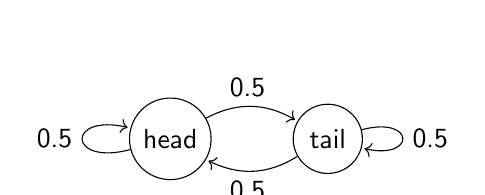
\begin{tikzpicture}[shorten >=1pt,node distance=2cm,on grid,auto] 
		\node[state] (s_1)   {head}; 
		\node[state] (s_2) [right=of s_1] {tail}; 
		%\node[state] (s_3) [below right=of q_0] {$s_3$}; 
		%\node[state](s_4) [below right=of q_1] {$s_4$};
		\path[->] 
		(s_1) edge [bend left=30]  node {0.5~~} (s_2)
		edge  [loop left] node {0.5} ()
		(s_2) edge  [bend left=30] node {0.5~~} (s_1)
		edge  [loop right] node {0.5} ();
		%(q_1) edge  node  {1} (q_3)
		%edge [loop above] node {0} ()
		%(q_2) edge  node [swap] {0} (q_3) 
		%edge [loop below] node {1} ();
		\end{tikzpicture}
	\end{center}

If instead we considered an unfair coin giving a head with a probability of $60\%$, then the Markov diagram would be: 
	\begin{center}
	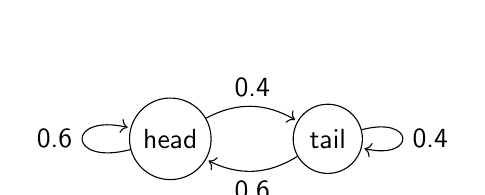
\begin{tikzpicture}[shorten >=1pt,node distance=2cm,on grid,auto] 
	\node[state] (s_1)   {head}; 
	\node[state] (s_2) [right=of s_1] {tail}; 
	%\node[state] (s_3) [below right=of q_0] {$s_3$}; 
	%\node[state](s_4) [below right=of q_1] {$s_4$};
	\path[->] 
	(s_1) edge [bend left=30]  node {0.4} (s_2)
	edge  [loop left] node {0.6} ()
	(s_2) edge  [bend left=30] node {0.6} (s_1)
	edge  [loop right] node {0.4} ();
	%(q_1) edge  node  {1} (q_3)
	%edge [loop above] node {0} ()
	%(q_2) edge  node [swap] {0} (q_3) 
	%edge [loop below] node {1} ();
	\end{tikzpicture}
\end{center}
\end{example}
	
	
	Another way to encode a this data is by means of a matrix, called a \textit{transition matrix}, which is particularly useful to understand the evolution over time of the process.
	
	\begin{df}{}
    The \textit{transition matrix} associated to a Markov diagram with $n$ states is the $n \times n$ matrix defined by:
	$$a_{i j} = \mbox{probablity of going from state $s_j$ at time $n$ to state $s_i$ at time $n+1$.}$$
	\end{df}
	
	
	
	\begin{example}
		\begin{itemize}
	\item[(i)]	The transition matrix associated to the fair flip coin above is: 
	$$A = \left(\begin{array}{cc} 0.5 &  0.5\\ 0.5 &  0.5 \end{array}\right),$$
	while the transition matrix associated to the unfair flip coin above is: 
	$$A = \left(\begin{array}{cc} 0.6 &  0.6\\ 0.4 &  0.4 \end{array}\right),$$
	\item[(ii)] The introductory example involving bikes can be modelled using a Markov diagram with four states $s_1, \ldots, s_4$ corresponding  to the four zones $1, \ldots, 4$ respectively. The associated transition matrix is: 
$$A =	\left(\begin{array}{cccc}
		0.5& 0.4 & 0.3 & 0.1\\ 0.2 & 0.2 &0.2 & 0.2 \\ 0.2& 0.2& 0.4 & 0.2 \\ 0.1& 0.2 & 0.1 & 0.5
	\end{array}\right).$$
	\end{itemize}
		\end{example}
	
	Note that a  transition matrix is a particular example of a stochastic matrix, as defined below: 
	
	\begin{df}{}
    An $n \times n$ matrix is called a \textit{stochastic matrix} if the following holds:
	\begin{itemize}
		\item[(S1)] $a_{ij} \geq 0$ for every $ 1 \leq i, j \leq n$,
		\item[(S2)] for every column $C_j$ of $A$, the sum of its entries is $1$.
	\end{itemize}
	\end{df}
	%To every \textit{finite Markov chain} consists of the following data: 
	%\begin{itemize}
	%	\item[(i)] a finite set $s_1, \ldots, s_n$ of \textit{states},
	%	\item[(ii)] a \textit{transition matrix} $A$.
	%\end{itemize}
	
	The transition matrix can be used to model the evolution over time of the distribution of a given number of elements taking at each time one of the possible states. Suppose that we start originally with $x_1$ elements in the state $s_1$, $x_2$ elements in the state $s_2$, etc. We encode this by a vector $\xv_0 = (x_1, \ldots, x_n)^T$, whose coordinates record the initial distribution of objects under study. At each iteration of the process, each object moves from one state to another with following the probabilities encoded in the Markov diagram (or equivalently, in the transition matrix). At a given time, we have the following:
	
	\begin{thm}{}
    Let $\xv_0 = (x_1, \ldots, x_n)^T$ be the vector whose coordinates record the initial distribution of elements in states $s_1, \ldots, s_n$. Let us denote by $\xv_k$ the vector whose components record the expected distribution after $k$ iterations of the process of elements in states $s_1, \ldots, s_n$ respectively. We have for every $k \geq 0$:
	$$ \xv_{k+1} = A\xv_k \mbox{ for every } k \geq 0.$$
	In particular, we get by induction: 
	$$\xv_k = A^k\xv_0.$$
	\end{thm}
	
	\begin{df}{}
		A vector $\xv$ such that $A\xv=\xv$ is called a \textit{stationary distribution}. In other words, it is an eigenvector of $A$ for the eigenvalue $1$.  
	\end{df}
	
A stationary distribution	represents the distribution over the possible states when the system is at equilibrium, i.e. does not change over time. 
	
	\begin{example} In the Markov chain modelling the distribution of bikes mentioned in the introduction, the vector $(70, 40, 50, 40)^T$ is a stationary distribution.
		\end{example}
	
	
	\subsection{The Perron-Frobenius Theorem for stochastic matrices}
	
	\begin{df}{}
    Let $A$  be an $n \times n$ matrix. 
		\begin{itemize}
			\item 	We say that $A$ is \textit{non-negative} if $a_{i j} \geq 0$ for every $i, j$, and \textit{positive} if $a_{i, j}>0$ for every $i, j$. 
			\item 	We say that a non-negative matrix $A$ is  \textit{regular} if $A^k $ is positive for some integer $k \geq 1$.
		\end{itemize}
%		We say that a matrix $A$ is \textit{non-negative} if $a_{i j} \geq 0$ for every $i, j$. We say that $A$  is \textit{positive} if $a_{i, j}>0$ for every $i, j$. 
%
%		A non-negative matrix $A$ is called \textit{regular} if $A^k $ is positive for some integer $k \geq 1$.
	\end{df}
	
		The transition matrix associated to a Markov diagram is non-negative, but not necessarily positive as there may be a probability $0$ of going from some state $s_i$ to some other state $s_j$.
	

		The integer $k$ in the definition above depends on the matrix. In particular, for every $k$ it is possible to construct a regular matrix $A$ such that $A^k$ is positive but $A, A^2, \ldots, A^{k-1}$ are not positive.
\begin{thm}{}
		The transition matrix associated to a Markov diagram is regular if and only if
%		 it possible to go from any state to any other state with non-zero probability. Equivalently, a finite Markov chain is regular if and only if 
		 there exists an integer $n \geq 1$ such that one can go from any vertex of its Markov diagram to any other by a sequence of exactly $n$ oriented edges.
	\end{thm}

\begin{proof}
	The $(i, j)$ term of $A^k$ is given by:
	$$(A^k)_{i, j} = \sum_{1 \leq i_1, \ldots, i_{k-1} \leq n} a_{i_{}, i_{1}}a_{i_{1}, i_{2}}\cdots a_{i_{k-2}, i_{k-1}}a_{i_{k-1}, j}.$$
	Since all the coefficients $a_{i, j}$ are non-negative, $A^k$ is positive if and only if for every $i, j$, there exists $1 \leq i_1, \ldots, i_{k-1} \leq n$ such that $a_{i_{}, i_{1}}a_{i_{1}, i_{2}}\cdots a_{i_{k-2}, i_{k-1}}a_{i_{k-1}, j}$ are all non-zero. Since a directed edge in the Markov diagram corresponds to a positive probability to move from one state to the other, this is equivalent to saying that for every $i, j$, there exists a sequence of $n$ directed edges from the state $i$ to the state $j$.
\end{proof}
	
	\begin{example}
		The following matrix is a regular stochastic matrix:
		$$A:= \left(\begin{array}{cc} 1/2 & 1/2  \\ 1/2 & 1/2  \end{array}\right).$$
		Indeed, it is clearly stochastic. Moreover, since $A = A^1$ is positive, it is also regular.
		\end{example}
	
	\begin{example} The following matrix is a regular stochastic matrix: 
		
	$$A:= \left(\begin{array}{cccc} 1/3 & 1/3 & 0& 1/3 \\ 1/3 & 1/3 & 1/3 & 0 \\0 & 1/3 & 1/3 & 1/3 \\1/3 & 0& 1/3 & 1/3 \end{array}\right).$$
	Indeed, the fact that $A$ is stochastic is clear, and we have: 
	$$A^2 = \left(\begin{array}{cccc}  1/3 & 2/9 & 2/9& 2/9 \\ 2/9 &  1/3 & 2/9& 2/9 \\2/9 & 2/9 &  1/3& 2/9\\2/9 & 2/9 & 2/9&  1/3 \end{array}\right),$$
	which is positive. 
	The corresponding Markov diagram is the following (where for simplicity we omit the probabilities, and we represent arrows from $s_i$ to $s_j$ and from $s_j$ to $s_i$ simply by a double arrow):
	
	\begin{center}
	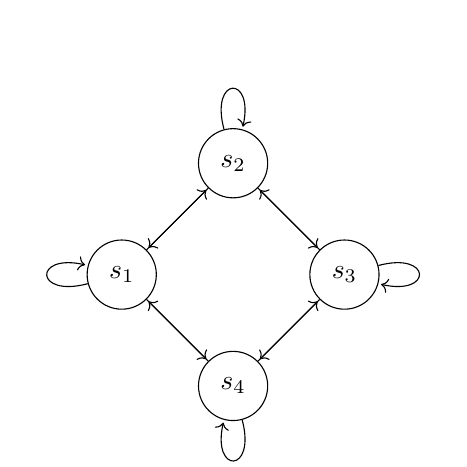
\begin{tikzpicture}[shorten >=1pt,node distance=2cm,on grid,auto] 
	\node[state] (s_1)   {$s_1$}; 
	\node[state] (s_2) [above right=of s_1] {$s_2$}; 
	\node[state] (s_3) [below right=of s_2] {$s_3$}; 
	\node[state](s_4) [below right =of s_1] {$s_4$};
	\path[->] 
	(s_1) edge [bend left=0]  node {} (s_2)
	edge [bend left=0]  node {} (s_4)
	edge  [loop left] node {} ()
	(s_2) edge [bend left=0]  node {} (s_1)
	edge [bend left=0]  node {} (s_3)
	edge  [loop above] node {} ()
	(s_3) edge [bend left=0]  node {} (s_2)
	edge [bend left=0]  node {} (s_4)
	edge  [loop right] node {} ()
	(s_4) edge [bend left=0]  node {} (s_1)
	edge [bend left=0]  node {} (s_3)
	edge  [loop below] node {} ();
	%(q_1) edge  node  {1} (q_3)
	%edge [loop above] node {0} ()
	%(q_2) edge  node [swap] {0} (q_3) 
	%edge [loop below] node {1} ();
	\end{tikzpicture}
\end{center}
	
	and we see that it is indeed possible to find a directed path of length $2$ between any pair of states. 
	\end{example}

	The key theorem of this chapter is the following:
	
	\begin{thm}{}
    Perron-Frobenius Theorem for stochastic matrices 
		Let $A$ be a regular stochastic matrix. Then the following holds: 
		\begin{itemize}
			\item[(i)] There exists stationary distributions for $A$. In other words, $1$ is an eigenvalue of $A$. 
			
			Moreover, there exists a stationary distribution all of whose components are strictly positive. 
				\item[(ii)] For every vector $\xv = (x_1, \ldots, x_n)^T$ such that $\sum_i x_i \neq 0 $, we have that the sequence of vectors $A^k\xv$ converges to a stationary distribution of $A$.
%			Such an eigenvector is called a \textit{Perron eigenvector}.
			\item[(iii)] $\dim E_1(A) = 1$.
			\item[(iv)] For every other eigenvalue $\lambda$ of $A$, we have $|\lambda|<1$.
		\end{itemize}
	\end{thm}
	

The proof of the Perron-Frobenius is rather long and technical (you can find the proof on the internet, or come and ask me after class/tutorials.). I will just present the proofs of two of the fours results, that illustrate nicely some of the concepts we have encountered in the course so far.

	

	For any square matrix, we have 
	$$\det(A^T) = \det(A).$$

	A square matrix and its transpose have the same eigenvalues.


\begin{proof}
	 Indeed, since $\det(A) = \det(A^T)$ for any square matrix, it follows that $$\chi_{A^T}(\lambda) = \det(A^T - \lambda I_n) = \det((A - \lambda I_n)^T) = \det(A- \lambda I_n) = \chi_A(\lambda).$$
	 	In particular, 
	 $$\lambda \mbox{ is an eigenvalue of } A \Longleftrightarrow \chi_A(\lambda)=0 \Longleftrightarrow \chi_{A^T}(\lambda) =0 \Longleftrightarrow \lambda \mbox{ is an eigenvalue of } A^T.$$
\end{proof}
	
	\begin{proof}
		(i) Notice that, since $A$ is stochastic, the entries in each column of $A$ add up to $1$. This can be reformulated as follows: 
		$$A^T \vecttt{1}{\vdots}{1} = \vecttt{1}{\vdots}{1}.$$
		In particular, we see that $1$ is an eigenvalue of $A^T$. But $A$ and $A^T$ have the same eigenvalues by the above theorem. 
%		Indeed, since $\det(B) = \det(B^T)$ for any square matrix by Proposition \ref{prop:det_transpose}, it follows that $$\chi_{A^T}(\lambda) = \det(A^T - \lambda I_n) = \det((A - \lambda I_n)^T) = \det(A- \lambda I_n) = \chi_A(\lambda).$$
%		In particular, 
%		$$\lambda \mbox{ is an eigenvalue of } A \Longleftrightarrow \chi_A(\lambda)=0 \Longleftrightarrow \chi_{A^T}(\lambda) =0 \Longleftrightarrow \lambda \mbox{ is an eigenvalue of } A^T.$$
		Since $1$ is an eigenvalue of $A^T$, it is also an eigenvalue of $A$.
		
		(ii) Let us prove this statement in the case where $A$ is diagonalisable. We choose a basis $\ev_1, \ldots, \ev_n$ of eigenvectors for the eigenvalues $1 = \lambda_1, \lambda_2, \ldots, \lambda_n$ respectively. Let $\xv \in \FR^n$ and let us write $\xv = \alpha_1\ev_1 + \ldots + \alpha_n\ev_n$,  for some $\alpha_1, \ldots, \alpha_n \in \FR$. We then have for $k \geq 1$: 
		\begin{equation*}
		\begin{aligned}
		A^k\xv &= \alpha_1A^k\ev_1 + \alpha_2A^k\ev_2 + \ldots + \alpha_nA^k \ev_n \\ & =  \alpha_1\ev_1 + \alpha_2\lambda_2^k\ev_2 + \ldots + \alpha_n\lambda_n^k \ev_n.
		\end{aligned}
		\end{equation*}
		Since $|\lambda_2|, \ldots, |\lambda_n| < 1$ by (iv), it follows that $A^k \xv$ converges to $\alpha_1\ev_1$. To conclude that the limit is an eigenvector (for the eigenvalue $\lambda_1=1$), it remains to show that $\alpha_1\ev_1 \neq \nv$. (an eigenvector cannot be the null vector.) But since $A$ is stochastic, the sum of the components of $A^k \xv$ remains the same at every stage. Since we started from a vector $\xv$ such that $\sum_i x_i \neq 0$, it follows that the sum of the components of $\alpha_1 \ev_1$ is non-zero, and in particular $\alpha_1\ev_1 \neq \nv$.
		\end{proof}
	%	The unique Perron eigenvector $\xv$ with $\sum_i x_i =1$ 
	
%	\paragraph{Speed of convergence.} In the case of a diagon
	
	\subsection{Application: stationary distributions in dynamical systems.}
	
		
	Let us go back to the problem stated in the introduction. The problem of modelling the changes in the distribution of bicycles can be modelled using a Markov diagram, whose transition matrix $A$ was given in the introduction. This associated transition matrix is regular, as it is positive. Let us denote by $\xv_0 = (50, 50, 50, 50)^T$ the vector corresponding to the initial distribution of bikes. After $k$ days, the expected distribution of bikes is given by $A^k\xv_0$. By (iv), this sequence of vectors converges towards a stationary distribution $\xv$. This stationary distribution is a vector whose components add up to $200$, since each vector $A^k\xv_0$ satisfies the same property (intuitively, the bikes are just redistributed, there is no gain nor loss of bike in the process). By (ii), since the eigenspace $E_1(A)$ is a line (i.e. has dimension $1$), there is a unique vector of $E_1(A)$ whose components add up to $200$, and this is exactly our stationary distribution $\xv$. Note that this characterisation of $\xv$ does not depend on the original distribution $\xv_0$. This explains in hindsight why the stationary distribution is unique, and does not depend on the original vector $\xv_0$. 
%	Consequences $(i)$ and $(iii)$ finally explain why there was exactly one stationary distribution of bicycles: such a distribution corresponds to the unique eigenvector of the transition matrix for the eigenvalue $1$ (we know that the associated eigenspace has dimension $1$) whose components add up to $200$, the total number of bikes.
%	
%	Moreover, consequence $(iv)$ justifies why starting from any distribution of bicycles, the distribution will evolve over time and converges to the unique stationary distribution just mentioned. 
	
	One natural question would be to understand the speed of convergence. When the transition $A$ matrix is diagonalisable, then there exists a basis $\ev_1, \ldots, \ev_n$ of $\FR^n$ for the associated eigenvalues $1 = \lambda_1 > \lambda_2 \geq \ldots \geq \lambda_n > -1$. In particular, if we write our initial vector $\xv$ as a linear combination of the $\ev_i$, as $\xv = \alpha_1\ev_1 + \ldots + \alpha_n\ev_n$,  we have for $k \geq 1$: 
	$$A^k\xv = \alpha_1\ev_1 + \alpha_2\lambda_2^k\ev_2 + \ldots + \alpha_n\lambda_n^k \ev_n.$$
	In particular, we see that $A^k\xv \ra_\infty \alpha_1\ev_1$ and  that   $||A^k\xv - \alpha_1\ev_1|| $ converges to zero exponentially, and as fast as $\mu^k$ (up to a multiplicative constant), where   
	 $$\mu = \underset{2 \leq i \leq n}{\mbox{max}}|\lambda_i|.$$
	 Rephrased using Landau's notations, we have: 
	 $$||A^k\xv - \ev_1|| = O(\mu^k)$$
	 If $A$ is not diagonalisable, a slightly weaker inequality holds, namely: 
	 $$||A^k\xv - \ev_1|| = o(\mu^k)$$
	 for every  
	 $ \underset{2 \leq i \leq n}{\mbox{max}}|\lambda_i| < \mu < 1.$ We will not prove this stronger statement in this course.
	
%	\paragraph{Linear economic models}
%	
%	As seen in the introduction of the first chapter, 
	
	\subsection{Application: The PageRank algorithm}
	
	

	
	One can imagine the internet as a (very large) oriented graph. Vertices correspond to pages and oriented edges correspond to links from a page to another. 
	
	To this oriented graph, we can associate a finite Markov chain whose states correspond to the pages, by assuming that a person on a given webpage will click with equal probability on one of the links of the page. To construct the associated transition matrix, we denote by $n_{ij}$ the number of links from page $j$ to page $i$, and by $d_j$ the total number of links on page $j$, then the probability $a_{ij}$ that someone on page $j$ clicks on a link leading to page $i$ is:
$$a_{ij} = \frac{n_{ij}}{d_j}.$$	
	Let us consider a small example of a very small network consisting of four webpages $p_1, \ldots, p_4$. The table representing the links between pages is given below, where the coefficient in row $i$ and column $j$ represents the number of links from page $j$ to page $i$:
	
	\begin{center}
				\begin{tabular}{l|llll}
			& $p_1$  & $p_2$  & $p_3$ & $p_4$ \\ \hline $p_1$ &
			0& 0& 2 & 2\\ $p_2$ & 2 & 0 &2 & 1 \\ $p_3$ & 1& 1& 0 & 2 \\ $p_4$ & 1& 1 & 1 & 0
		\end{tabular}
	\end{center}

	
	The transition matrix associated to this Markov chain is:
	
	$$A=  \left(\begin{array}{cccc}
	0& 0& 2/5 & 2/5\\ 1/2 & 0 &2/5 & 1/5 \\ 1/4& 1/2& 0 & 2/5 \\ 1/4& 1/2 & 1/5 & 0
	\end{array}\right).$$
	
	

	
	However, this model  fails to take into account that quite often people will go to a webpage not because it was linked from a previous page, but because they started thinking of something completely different, independently of the content of the current page. This can be modelled by another Markov process where at each time, the probability of going from any page to any other page is exactly $1/n$, where $n$ is the number of pages (in our example, $n=4$). This finite Markov chain has a transition matrix a $n \times n$ matrix of the form
	
	$$U = \left( \begin{array}{ccc}1/n & \cdots & 1/n\\ \vdots & \ddots & \vdots \\ 1/n & \cdots & 1/n \end{array}\right).$$
	
	What Google does to take both processes into consideration is to consider that what is going on is a combination of the previous cases. There exists a constant $\alpha$, called \textit{damping factor}, such that with probability $\alpha$, a person will choose the next page by clicking on one of the links, and with probability $(1-\alpha)$ that person will choose the next page completely at random. A standard value for $\alpha$ is $\alpha=0.85$. This corresponds to a Markov process whose transition matrix is given by the following barycenter of $A$ and $U$: 
	$$G:= \alpha A + (1-\alpha) U.$$ 
	Note that this transition matrix is now strictly positive, and in particular regular. We can thus apply the Perron-Frobenius Theorem, which tells us that there exists a stationary distribution with positive components and with sum $1$, called the \textit{ranking vector}. By the convergence property, this corresponds to the expected distribution of people on pages when this process has been repeated infinitely many times. Pages with a comparatively high distribution correspond to `popular' pages, and are thus ranked highly by Google. This ranking vector is (a simplified version of) what Google uses to rank pages. 
	
	\begin{df}{}
		A \textit{ranking vector} used in the Google PageRank algorithm is a stationary distribution of the `Google matrix' $G = \alpha A + (1-\alpha) U$ with positive components. (Such a vector is unique up to multiplication by a positive constant, by the Perron-Frobenius Theorem)
		
		 The ranking of the webpages is obtained by ranking the components of that vector.
		\end{df}
	
	Let us go back to our simple example. Taking the damping factor to be $0.85$, the new transition matrix for the process is
	\begin{equation*}
	\begin{aligned}
	G ~~~&= ~~~0.85 \left(\begin{array}{cccc}
	0& 0& 2/5 & 2/5\\ 1/2 & 0 &2/5 & 1/5 \\ 1/4& 1/2& 0 & 2/5 \\ 1/4& 1/2 & 1/5 & 0
	\end{array}\right) + 0.15 \left(\begin{array}{cccc}
	1/4& 1/4 & 1/4 & 1/4\\ 1/4& 1/4 & 1/4 & 1/4 \\ 1/4& 1/4 & 1/4 & 1/4 \\ 1/4& 1/4 & 1/4 & 1/4
	\end{array}\right)\\
	 &= ~~~  \left(\begin{array}{cccc}
	 0.0375& 0.0375& 0.3775 & 0.3775\\ 0.4625 & 0.0375 &0.3775 & 0.2075 \\ 0.25& 0.4625& 0.0375 & 0.3775 \\ 0.25& 0.4625 & 0.2075 & 0.0375
	 \end{array}\right).
	\end{aligned}
	\end{equation*}
	
	Finding the stationary distribution corresponds to solving the system $G\xv = \xv$, which we do as usual using Gaussian elimination, with a computer as the computations are too cumbersome. The  unique stationary distribution $\rv$ whose components are positive and add up to  $1$ is  (with approximations to the second digit)
	$$\rv ~\simeq ~\vectttt{0.21}{0.26}{0.28}{0.24}.$$
	So the ranking of these pages, from most popular to least popular, is: page $3$, page $2$, page $ 4$, page $ 1$.
	
	\paragraph{Speed of convergence (extra-curricular).} We know from the Perron-Frobenius Theorem that a way to obtain a ranking vector is to look at the asymptotic behaviour of $G^k \xv$ for an arbitrary vector $\xv$ with $\sum x_i =1$. We wish to find an upper bound on the norm $ ||G^k\xv -  \rv ||$. However,instead of looking at this norm, we will be looking at a slightly different one that is easier to use in this situation: 
	
	$$ ||\xv||_1  = \sum_i |x_i|.$$
	Note that we still have the triangle identity $||\xv + \yv||_1 \leq ||\xv||_1 + ||\yv||_1$. Moreover, for every  vector $\xv = (x_1, \ldots, x_n)^T$, we have:
	$$||A\xv||_1 = \sum_i | \sum_j a_{i j}x_j | \leq \sum_i \sum_j a_{i j}|x_j|  \leq  \sum_j |x_j| (\sum_i a_{i j})  \leq \sum_i |x_i| = ||\xv||_1.$$
	
	\begin{thm}
		For every $k \geq 1$ and every positive vector $\xv$ whose components add up to $1$, we have:
		$$||G^k\xv -  \rv ||_1  \leq  2\alpha^k.$$
		\end{thm}
	
	\begin{proof} We have: 
	
	$$G\xv = \alpha A\xv + (1-\alpha)U\xv = \alpha A\xv + (1 - \alpha) \vecttt{1/n}{\vdots}{1/n}.$$
	
	In particular, for non-negative vectors $\xv, \yv$, we get 
	
	$$G\xv - G\yv = \alpha A(\xv - \yv),$$
	and $$||G\xv - G\yv||_1 = \alpha ||A(\xv - \yv)||_1 \leq \alpha ||\xv - \yv ||_1.$$
	By induction, we get 
	$$||G^k\xv - G^k\yv||_1  \leq \alpha^k||\xv - \yv ||_1$$
	and thus, for every positive vector $\xv$ whose components add up to $1$, we get:
	$$||G^k\xv -  \rv ||_1  = ||G^k\xv -  G^k\rv ||_1 \leq \alpha^k||\xv - \rv ||_1\leq \alpha^k(||\xv||_1 + ||\rv||_1)\leq  2\alpha^k.$$	\end{proof}
	Note in particular that this speed of convergence is independent on the size of the matrix. For instance, for $\alpha = 0.85$, then the power method gives an approximation of the ranking vector with error less than $10^{-6}$ after $ 90$ iterations. 
%	\paragraph{Approximating non-regular matrices by regular ones.} h


\appendix

%\newpage
%\section{Answer to (most) Tutorial Exercises}
%\label{A:answers}
%\shipoutAnswer
%\newpage
\pagestyle{empty}
\newgeometry{left=25mm,right=25mm,top=2cm,bottom=20mm}
\section{Formula Sheet}
\label{A:Formula}
\vspace{-2ex}

\begin{multicols}{2}
\begin{center}
\textbf{Trigonometrical Identities}
\end{center}
\vspace{-2ex}
{\footnotesize
\begin{align*}
\sin^2(A) +\cos^2(A) &= 1\\
\sin(A\pm B)&= \sin(A)\cos(B) \pm \cos(A)\sin(B)\\
\cos(A\pm B)&= \cos(A)\cos(B) \mp \sin(A)\sin(B)\\
\sin(2A) &= 2\sin(A)\cos(A)\\
\cos(2A) &= 2\cos^2(A)-1 = 1-2\sin^2(A)\\
2\sin(A)\cos(B)&= \sin(A+B) + \sin(A-B)\\
2\cos(A)\sin(B)&= \sin(A+B) - \sin(A-B)\\
2\cos(A)\cos(B)&= \cos(A+B) + \cos(A-B)\\
2\sin(A)\sin(B)&= \cos(A+B) - \cos(A-B)
\end{align*}
}%
\vfill

\begin{center}
\textbf{Hyperbolic Functions}
\end{center}
\vspace{-2ex}
\begin{align*}
\sinh(x) &= \frac{e^x - e^{-x}}{2}\\
\cosh(x) &= \frac{e^x + e^{-x}}{2}\\
1&=\cosh^2(x) - \sinh^2(x)\\
\sinh(2x) &= 2\sinh(x)\cosh(x)\\
\cosh(2x) &= 2\sinh^2(x)+1=2\cosh^2(x)-1
\end{align*}

\vfill

\begin{center}
\textbf{Standard Derivatives}
\end{center}
\vspace{-1ex}
{
\renewcommand{\arraystretch}{2.2}
\begin{center}
\begin{tabular}{|c|c|} 
\hline
$f(x)$ & $f'(x)$\\ 
\hline \hline
$x^n$ & $nx^{n-1}$\\
\hline
$\sin (ax + b)$ & $a\cos (ax + b)$\\
\hline
$\cos (ax + b )$& $- a\sin ( ax + b)$\\ 
\hline
$e^{ax}$  & $ae^{ax}$\\ 
\hline
$\ln(a x + b )$&   $\frac{a}{ a x + b}$ \\
\hline
$\sinh (ax + b)$ & $a\cosh (ax + b)$\\
\hline
$\cosh (ax + b)$ & $a\sinh (ax + b)$\\
\hline
$uv$ & $u'v+uv'$\\
\hline
$\displaystyle \frac{u}{v}$ & $\displaystyle \frac{u'v-uv'}{v^2}$\\
\hline
\end{tabular}
\end{center}
}

\vfill\null
\columnbreak

\begin{center}
\textbf{Standard Integrals}
\end{center}
\vspace{-1ex}
{
\renewcommand{\arraystretch}{2.2}
\begin{tabular}{|c|c|}
\hline
$f(x)$ & $\displaystyle \int f(x) dx$ \\
\hline \hline
$x^n$ & $\displaystyle \frac{x^{n+1} }{n+1}  + C$  for $n\neq -1$  \\ \hline
$(ax+b)^n$ & $\displaystyle \frac{(ax+b)^{n+1} }{a(n+1)}  + C$  for $n\neq -1$  \\ \hline
$\sin (a x +b)$ &  $\displaystyle -\frac{1}{a} \cos ( a x+ b) + C$\\ \hline
$\cos (a x +b)$ &  $\displaystyle \frac{1}{a} \sin (a x +b) + C $\\ \hline
$e^{a x}$ & $\displaystyle \frac{1}{a} e^{ax} + C$ \\ \hline
$\displaystyle \frac{1}{ ax + b}$ & $\displaystyle \frac{1}{ a} \ln (ax +b)  + C$ for $ax+b>0$ \\ \hline
$\displaystyle \cosh(x)$ & $\displaystyle \sinh(x)  + C$ \\ \hline
$\displaystyle \sinh(x)$ & $\displaystyle \cosh(x)  + C$ \\ \hline \hline
$\displaystyle \frac{1}{x^2+a^2}$ & $\displaystyle \frac{1}{a}\arctan\left(\frac{x}{a}\right) + C$\\ \hline
$\displaystyle \frac{1}{\sqrt{a^2-x^2}}$ & $\displaystyle \arcsin\left(\frac{x}{a}\right) + C$\\ \hline
$\displaystyle \frac{1}{a^2-x^2}$ & $\displaystyle \frac{1}{2a}\ln\left(\frac{a+x}{a-x}\right) + C$\\ \hline
$\displaystyle \frac{1}{x^2-a^2}$ & $\displaystyle \frac{1}{2a}\ln\left(\frac{a-x}{a+x}\right) + C$\\ \hline
$\displaystyle \frac{1}{\sqrt{x^2+a^2}}$ & $\displaystyle \ln\left(x+\sqrt{x^2+a^2}\right) + C$\\ \hline
$\displaystyle \frac{1}{\sqrt{x^2-a^2}}$ & $\displaystyle \ln\left(x+\sqrt{x^2-a^2}\right) + C$\\ \hline\hline
$\displaystyle u v'$ & $\displaystyle uv - \int u' v dx$\\ \hline
\end{tabular}
}

\end{multicols}

%\restoregeometry

\end{document}

